\documentclass[12pt]{gatech-thesis}
\usepackage{amsmath,amssymb,latexsym,float,epsfig,subfigure}
\usepackage{booktabs}
\usepackage{multirow}
\usepackage{siunitx}
\usepackage{amsmath}
\usepackage{lscape}
\usepackage{listings}

\usepackage{savesym}
\savesymbol{pdfbookmark}
\usepackage[hidelinks]{hyperref}
\restoresymbol{HR}{pdfbookmark}

%\usepackage[round]{natbib}
\newcolumntype{x}[1]{>{\raggedleft\hspace{0pt}}p{#1}}

%%
%% This example is adapted from ucthesis.tex, a part of the
%% UCTHESIS class package...
%%
%\title{Behavior Design and Representations For a People Aware Mobile Robot System} %% If you want to specify a linebreak

\title{Navigation Behavior Design and Representations For a People Aware Mobile Robot System}

                               %% in the thesis title, you MUST use
                               %% \protect\\ instead of \\, as \\ is a
                               %% fragile command that \MakeUpperCase
                               %% will break!
\author{Akansel Cosgun}
\department{College of Computing}

%% Can have up to six readers, plus principaladvisor and
%% committeechair. All have the form
%%
%%  \reader{Name}[Department][Institution]
%%
%% The second and third arguments are optional, but if you wish to
%% supply the third, you must supply the second. Department defaults
%% to the department defined above and Institution defaults to Georgia
%% Institute of Technology.

\principaladvisor{Professor Henrik Iskov Christensen}
%\committeechair{Professor Ignatius Arrogant}
\firstreader{Professor Andrea Thomaz}[College of Computing]
\secondreader{Professor Irfan Essa}[College of Computing]
\thirdreader{Professor Ayanna Howard}[School of Electrical and Computer Engineering]
\fourthreader{Dr Emrah Akin Sisbot}[Toyota InfoTechnology Center][]
%\setcounter{secnumdepth}{2}
\degree{Doctor of Philosophy}

%% Set \listmajortrue below, then uncomment and set this for
%% interdisciplinary PhD programs so that the title page says
%% ``[degree] in [major]'' and puts the department at the bottom of
%% the page, rather than saying ``[degree] in the [department]''

%% \major{Algorithms, Combinatorics, and Optimization} 

\copyrightyear{2016} 
\submitdate{May 2016} % Must be the month and year of graduation,
                         % not thesis approval! As of 2010, this means
                         % this text must be May, August, or December
                         % followed by the year.

                                                                                                                                                                                                                                                                                                                                                                                                                                                                                                                                                                                                                                                                                                                                                                                                                                                                                                                                                                                                                                                                                                                                                                                                                                                                                                                                                                                                                                                                                                                                                                                                                                                                                                                                                                                                                                                                                                                                                                                                                                                                                                                                                                                                                                                                                                                                                                                                                                                                                                                                                                                                                                                                                                                                                                                                                                                                                                                                                                                                                                                                                                                                                                                                                                                                                                                                                                                                                                                                                                                                                                                                                                                                                                                                                                                                                                                                                                                                                                                                                                                                                                                %% The date the last committee member signs the thesis form. Printed
%% on the approval page.
\approveddate{1/11/2016}

\bibfiles{example-thesis}

%% The following are the defaults
%%    \titlepagetrue
%%    \signaturepagetrue
    \copyrighttrue
%%    \figurespagetrue
%%    \tablespagetrue
%%    \contentspagetrue
%%    \dedicationheadingfalse
%%    \bibpagetrue
%%    \thesisproposalfalse
%%    \strictmarginstrue
%%    \dissertationfalse
%%    \listmajorfalse
%%    \multivolumefalse


\begin{document}
%\bibliographystyle{plainnat}
\bibliographystyle{gatech-thesis}
%%
\begin{preliminary}

% Dedication
\begin{dedication}
\null\vfil
{\large
\begin{center}
To my parents,\\\vspace{12pt}
Zeynep and Huseyin Co\c{s}gun,\\\vspace{12pt}
who are my pillars of strength;\\\vspace{12pt}
and to my wife Gamze,\\\vspace{12pt}
who always supports me, rain or shine.\\\vspace{12pt}
\end{center}}
\vfil\null
\end{dedication}


%\begin{preface}
%Preface
%\end{preface}

\begin{acknowledgements}

First, I would like to thank my colleagues at IRIM, especially to Alex Trevor, Victor Emeli, Baris Akgun and Can Erdogan, for useful research discussions an their friendship.

Thanks to my committee for their helpful comments and feedback: Andrea Thomaz, Ayanna Howard and Irfan Essa. Thanks to Akin Sisbot, who also is on my committee, for his close collaboration at Toyota and setting the standard in this line of research. Thanks to Dinei Floriencio his mentorship during my time at Microsoft. Moreover, thanks to the Korea Industrial Technology Foundation, The Boeing Company, BMW, Peugeot S.A. and ThyssenKrupp for financially supporting the body of work in this thesis.

I would like to remember Mike Stilman, whose passing was a shock to all of us. I wrote my first research paper under his helpful guidance and his enthusiasm was contagious.

Finally, special thanks to my thesis advisor Henrik Christensen, for his to-the-point comments and proper advice, and being a role model to me with his fair management style and charisma.

\end{acknowledgements}
\contents
\begin{summary}

There are millions of robots in operation around the world today, and almost all of them operate on factory floors in isolation from people. However, it is now becoming clear that robots can provide much more value assisting people in daily tasks in human environments. Perhaps the most fundamental capability for a mobile robot is navigating from one location to another. Advances in mapping and motion planning research in the past decades made indoor navigation a commodity for mobile robots. Yet, questions remain on how the robots should move around humans. This thesis advocates the use of semantic maps and spatial rules of engagement to enable non-expert users to effortlessly interact with and control a mobile robot.

A core concept explored in this thesis is the Tour Scenario, where the task is to familiarize a mobile robot to a new environment after it is first shipped and unpacked in a home or office setting. During the tour, the robot follows the user and creates a semantic representation of the environment. The user labels objects, landmarks and locations by performing pointing gestures and using the robot's user interface. The spatial semantic information is meaningful to humans, as it allows providing commands to the robot such as ``bring me a cup from the kitchen table". While the robot is navigating towards the goal, it should not treat nearby humans as obstacles and should move in a socially acceptable manner.

Three main navigation behaviors are studied in this work. The first behavior is the point-to-point navigation. The navigation planner presented in this thesis borrows ideas from human-human spatial interactions, and takes into account personal spaces as well as reactions of people who are in close proximity to the trajectory of the robot. The second navigation behavior is person following. After the description of a basic following behavior, a user study on person following for telepresence robots is presented. Additionally, situation awareness for person following is demonstrated, where the robot facilitates tasks by predicting the intent of the user and utilizing the semantic map. The third behavior is person guidance. A tour-guide robot is presented with a particular application for visually impaired users.

\end{summary}
\end{preliminary}

\chapter{Introduction}
\label{chapter:introduction}

\section{Robots in Human Environments}

The vision that was promised by Karel \v{C}apek in his 1921 science fiction play R.U.R, in which the word \textit{``robot"} was used the first time, featured intelligent autonomous systems that co-existed and worked for humans. The reality almost a century later today is that robots do exist, however almost all of them operate in factories, physically separated from human workers. With this separation, the safety of humans is ensured. However, it is now becoming clear that robots can provide much more value if they operate in human environments, assisting people in daily tasks. With the recent improvements in hardware and software systems and in robotics research, development of such robots is not science fiction anymore. This disruptive technology will make fascinating new applications possible, in contexts such as homes, hospitals, offices and factories, including but not limited to: delivery, elderly care, collaborating on an assembly line and household tasks such as cleaning. The feasibility and reliability of such applications will determine their business value, while potentially generating a new industry. Therefore, any development in this field is a step toward realization of \textit{intelligent} and \textit{social} robots.

\section{Robots that Navigate in Human Environments}

The most important difference of a robot from a computer is actuation: the ability to move around in the physical world. Perhaps the most fundamental task for a mobile robot is \textit{navigation} from one location to another. Advances in mapping, localization and path planning research in the past decades made indoor navigation a common capability for mobile robots. 

Robots occupy the same physical space with us, therefore should be aware of the fact that their movements would be observed and reacted by humans. Investigating the context of robots in human environments gave rise to the sub-field of robotics: Human-Robot Interaction (HRI). This relatively new research field extends in many directions with a common goal: robots that will perceive its environment, reason and act in a safe way to facilitate people's lives. Thus, a robot that will serve to people should not only be a machine, but should respect social rules and protocols.

\section{The Science of Personal Spaces}
\label{sec:personal_spaces}

How should mobile agents adjust their spatial relationships with respect to humans? In fact, humans already have a framework for this problem. It is called the \textit{proxemics}, coined by Hall \cite{hall1966hidden}, which studies of our use of space and the degree and effect of the spatial separation individuals naturally maintain. One of Hall's main findings is that humans adjust their distance in four distance levels: intimate, personal, social and public distances, depending on the intimacy level between individuals.

Personal spaces are influenced by other factors such as cultures, the range of their sensory systems, and postures of the two actors. Although it is not known whether it is best to model robot navigation behaviors after humans, using human-human studies to determine the spatial relationships to humans is a good start. This is especially true given that non-expert users today never interacted with a mobile robot and thus are likely expect the robot to behave within human social norms.

\section{Tour Scenario}
\label{sec:tour_scenario}

A mobile robot must first acquire the model of its environment before being tasked with navigation. In human environments, one method to familiarize the robot to a new environment is via \textit{Tour Scenario} \cite{topp2008human}. With the Tour Scenario, the robot interactively collects semantic information in an environment. Here is how the Tour Scenario is defined: After the robot product is shipped and unpacked to a home or similar environment, a human user takes the robot on a tour so the robot can create a representation of the environment. In this interactive scenario, the robot learns basic information about the surroundings, while following the user. During the tour, the user can point out and identify relevant places and objects which the robot can utilize for future tasks. It is likely that the a commercial robot product that has the capability of the familiarizing task will include both human-interactive and automatic components (i.e. automatic object recognition). In this thesis we focus on the interactive components.

\section{Semantic Maps}
\label{sec:semantic_maps}

Robots keep a representation of its environment to enable navigation behaviors, and it is usually in the form of a discrete metric \textit{map}, where each grid cells represent whether that position is occupied with an obstacle or not. Mobile robots that use such a map can accept navigation goals in metric coordinates (i.e. go to coordinate (5.2, -1.3)), however it may not be the most intuitive way to communicate goals for human users. Robots that navigate in human environments will need to accept human-friendly navigation goals. A map for such robots should act as a \textit{common ground} between the robot and its user, by enabling referencing to the same spatial elements. For example, the robot should be able to understand commands such as ``go to the kitchen table" or ``wait outside Joe's room". This is only possible with a richer map representation that includes \textit{semantic} information. In particular, if the humans and robots need to communicate over navigation goals that involve objects, landmarks or rooms, a map should include information about these.

\section{Challenges}

There are four primary challenges in developing practical systems that allow a real robotic system to navigate using semantic information. From the robot's perspective, the interesting research questions are:

\begin{itemize}
\item Where are the people?
\item How should I move around humans?
\item How can I acquire semantic information about this environment?
\item How can I utilize this semantic information to improve navigation?
\end{itemize}

The challenges laid by these questions will be addressed for the remainder of this section. The answers to the research questions are discussed throughout this thesis.

\subsection{Robust People Tracking}

In order to be engaged in any kind of meaningful spatial interaction with people, the robot has to be able to track them. Robust tracking of people is necessary to ensure high task rates.

We use a person tracking system that fuses detections from three sources. These three detectors are: leg detector, torso detector and upper body detector. Use of multiple modalities is leveraged to increase the robustness of tracking and provide more coverage around the robot. The detections are consolidated into position estimations using a Kalman Filter.

\subsection{Social Navigation}

Robot path planing for navigation has been traditionally considered as a shortest-path problem. While this leads to correct and collision-free paths, the behavior of the robot may be perceived as unsafe or unnatural by human observers. When a robot is navigating in an human environment, the most important consideration is the safety of people. Moreover, even if a robot's motions are safe, they can still cause discomfort. For example, sudden appearance of a robot can cause fear in humans or cutting in between two people while they are in a conversation may be considered a rude behavior. Therefore, the robot motions should not only be effective but also be socially acceptable.
%\label{sec:home_tour_scenario}
Borrowing the idea from Sisbot \cite{sisbot2007human}, we embed personal spaces and social constraints as costs while planning a path. We further develop the planner by considering simulating people's reaction to robot's motion during planning. Humans routinely use anticipation during navigation. For example, in a hallway encounter, one may lean towards the left of the corridor, expecting the other person to take right. We aim to give this anticipation ability to robots. Furthermore, we develop applications where the goal of the robot is to follow a person or a guide a person.

\subsection{Interactive Map Annotation}

The question of how semantic maps could be useful for various tasks is addressed in Section \ref{sec:tour_scenario}. Users may want to provide custom labels to landmarks, objects and waypoints instead of generic ones. By using unique labels, ambiguities can be resolved. For example, if an automatic object recognizer is utilized, the robot may be confused if it is given the command ``bring my laptop" and there are multiple laptops in the environment.

Moreover, the ability to label objects and then refer to them relieves the robot the burden to have a strong recognizer. Without any object recognition capability, a user can point at and label an object and later refer to it while tasking. For example, an object that was previously labeled as ``Joe's mug" can be retrieved with a command such as ``Fetch Joe's mug from the kitchen table".

A solution to enable a common ground between the user and the robot is via the Tour Scenario, as described in Section \ref{sec:tour_scenario}. For this scenario, the robot follows the user throughout the tour.

\subsection{Situation Awareness for Navigation}

Metric maps provide a single type of information: whether a grid cell is occupied with an obstacle or not. While this kind of a simplistic map representation may be sufficient for some tasks, if the robot needs to communicate with human users about its goals, it should have a richer map representation of the environment. The robot can leverage the semantic information embedded to the map and increase its usefulness for navigation tasks. %There are not many works in the field that tapped into this opportunity.

%None of the works in this field leverage the semantic maps to increase situational awareness.

Situation awareness of the robot can be achieved in different ways. Person following is a widely studied behavior, however in the literature it is not usually considered \textit{why} the robot is following the person and how the task context can be used to increase effectiveness. For example, during the Tour Scenario, the robot may employ a better following strategy if it knows the user will be pointing at landmarks and places. Furthermore, consider handling of the doors while following. If the robot does not know that it is standing on a doorway, it can block the path for others. If the door is added to the semantic map, the robot can have the opportunity to handle the door passing graciously. Moreover, the robot can utilize the map to adjust its speed. For example, if the robot is in a region where the chance to encounter a person is high, slowing down may be a sensible action to take.


%For example, when the robot is navigating, if the robot knows that it is in a region of high human density, slowing down may be a sensible action to take.



%Goal Points
%Door, landmarks, objects as special cases.
%Safety: Use map layout for speed adjustments, speed up

\section{Scope and Context}

In this section, we provide an overview of the assumptions of our research.  At a high level, autonomous robots perceive its environment, reason the situation, act in the world. In the HRI context, the research in perception is focused on improving the robot's ability to ``see" its environment, identify objects and humans. The reasoning part is focused on deciding on ``what to do" and ``how to do" in a given situation. Acting part is focused on the execution and control of motions from the reasoning part as well as the design of mechanisms. This thesis focuses on the reasoning part while also contributing to the perception part.

We assume that we have wheeled mobile robot platform. Even though some of our algorithms are derived for non-holonomic robots (differential drive), it is a technical limitation than a conceptual one, as they can be applied to holonomic robots with minor changes. We further assume that the robot is self-contained: equipped with on-board sensors, is capable of creating a map of the environment with an existing Simultaneous Localization and Mapping (SLAM) package, and then able to localize itself in this created map as it moves in the environment.

Furthermore, we focus on scenarios where people in the environment are standing or walking, because that's the most common body pose to encounter when the mobile robot is in motion.

The interaction between the robot and user is achieved via tablet or smartphone apps. Similar functionality could be achieved via a speech dialog system, however we chose touch-based interfaces due to their ubiquity and high reliability.

\section{Thesis Overview}
\subsection{Thesis Statement}

%Non-expert users can label objects, landmarks and locations while giving a tour to a mobile robot, where the labeled entities enable situational awareness and serve as end goals, which robots can navigate to, by taking into account the personal spaces of nearby humans and social factors.

Non-expert users can effortlessly interact with and control a mobile robot through the use of semantic maps and spatial rules of engagement.

\subsection{Contributions}

\begin{itemize}
%\item Development of a multimodal person detection and tracking system using on-board sensing, with a particular focus on 360$^{\circ}$ coverage
\item A method for a human to take a mobile robot on a tour and interactively add labeled objects, landmarks and locations to the robot's map using natural deictic gestures and later use these labeled entities as end goals for navigation
\item Development of a navigation planner that takes into account social factors, and reactions of people to robot's motions
\item Development of a person guidance behavior and its application to indoor wayfinding for blind users
\item Development of a person following behavior and its usage for telepresence robots
\item Demonstration of situation awareness for person following behavior, targeted at the Tour scenario
\end{itemize}


\subsection{Document Outline}

The rest of this document is organized as follows.

\textbf{Chapter \ref{chapter:map_annotation} - Map Annotation} describes our semantic map representation, the process of interactively labeling landmarks, the user interface and how we detect pointing gesture targets.

\textbf{Chapter \ref{chapter:multimodal_person_detection_and_tracking}- Multimodal Person Detection and Tracking} presents our method of leg detection, torso detection and face recognition and how the robot estimates the positions of nearby people using these detections.

\textbf{Chapter \ref{chapter:navigation_among_people} - Navigation Among People} discusses how we extract goal points from semantic maps, and a people-aware planner for navigating from a position to another.

\textbf{Chapter \ref{chapter:person_following} - Person Following} describes how the robot follows a person, uses semantic landmarks to handle special cases during following and discusses application to telepresence robots.

\textbf{Chapter \ref{chapter:person_guidance} - Person Guidance} presents a tour-guide robot and its application to particular use for blind users.

\textbf{Chapter \ref{chapter:conclusion} - Conclusion and Discussion} re-iterates contributions of this thesis and discusses open questions in this area of research.

\chapter{Multimodal Person Detection and Tracking}
\label{chapter:multimodal_person_detection_and_tracking}
The ability to robustly track a person is an important prerequisite for human-robot interaction. To realize any task that involves humans, the challenge is the detection and tracking of humans in the vicinity of the robot considering the robot's movements, sensing capabilities and occlusions. The scope of how much information is needed from the human perception module depends on the objective of the application. First, the robot should determine if there are people nearby. If the robot senses people around, the robot should find out \emph{where} they are. Representing people as points (x,y) in maps is common practice for navigation planning. If the task requires the robot to face a person, then the orientation $\theta$ needs be detected. The robot further can determine \emph{who} the detected person is. Identification of humans is necessary for enabling non-generic service. Finally, the robot should interpret \emph{what} the person is doing by analyzing the motion features and through gesture analysis. Tracking body parts of humans over time give significant information about human activity.

We focus on tracking people who are either walking or standing, as these are the two most common human poses around a mobile robot. Many full-body or body part detectors have been developed in the literature, reviewed in Section~\ref{sec:multimodal_related_work}. Full-body detectors are not suitable for mobile robot navigation applications because of their inability of capturing the entire body with on-board sensors when people are close to the robot. We aim to robustly track a person $360^{\circ}$ around the robot. However, most sensors have a limited field of view and using only a single detector can lead to a system with a single point of failure. Therefore, we think a multimodal detection system is better suited for on-board people tracking for our use cases. 

Laser scanners are the natural sensor of choice as state-of-the-art mobile robots are already equipped with an ankle-height laser scanner that is mainly used for navigation. The laser scanners we used on our robot are Hokuyo UTM 30-LX, which has $270^{\circ}$ Field of View (FOV), $0.25^{\circ}$ angular resolution, $40Hz$ refresh rate and $30m$ maximum range. We are only interested in detections in close range (less than $5m$). In that range interval, and the accuracy of each laser reading is $\pm 3cm$, which is sufficient for our use cases. The relatively higher accuracy and resolution are the two advantages of laser scanners over cameras and RGB-D cameras. Cameras, on the other hand, have the advantage of providing richer information, which can be used to extract body parts. We use a combination of detectors using either a laser scanner and RGB-D camera for robustness and better coverage, described in Section~\ref{sec:multimodal_person_detection}. Representing people as a points in the map is sufficient for mobile robot navigation and each detector produces a point as a person hypothesis. We use a real-time probabilistic tracking framework that relies on the fusion of the multiple person detections, described in Section~\ref{sec:multimodal_person_state_estimation}. For certain applications, identifying specific users allows the robot to go beyond generic capabilities. We present our face recognition method in Section~\ref{sec:multimodal_face_recognition}.

\section{Related Work}
\label{sec:multimodal_related_work}

Person detection was first addressed by the computer vision community as an object detection problem. Early research on person detection using vision is surveyed by Moeslund \cite{moeslund2001}. Face detection is a common method for detecting people, with the work of Viola and Jones \cite{viola2004robust} being the most popular one. See Zhang \cite{zhang2010survey} for a survey on contemporary approaches on vision based face detection. Another popular topic has been pedestrian detection in crowded scenes Leibe \cite{leibe2005pedestrian} and Tuzel \cite{tuzel2007human}.

In 2000's, laser scanners became the de-facto sensor for localization and mapping. Laser scanners are usually placed slightly above floor for obstacle avoidance, therefore leg detection is common practice. Early works by Montemerlo \cite{montemerlo2002conditional} and Schulz \cite{schulz2001tracking} focused on tracking multiple legs using particle filters. Legs are typically distinguished in laser scans using geometric features such as arcs \cite{xavier2005fast} and boosting can be used to train a classifier on a multitude of features \cite{arras2007using}. Topp \cite{topp2005tracking} demonstrates that leg tracking in cluttered environments is prone to false positives. For more robust tracking, some efforts fused information from multiple lasers such as Carballo's work \cite{Carballo2008}, which uses a second laser scanner at torso level. Glas \cite{glas2009laser} uses a network of laser sensors at torso height in hall-type environments to track the position and body orientation of multiple people. Several works used different modalities of sensors to further improve the robustness. Kleinehagenbrock \cite{kleinehagenbrock2002person} and Bellotto \cite{bellotto2009multisensor} combine leg detection and face tracking in a multi-modal tracking framework. Other examples include combining sound localization and vision \cite{bernardin2007audio} and combining RFID tracking and vision \cite{germa2010vision}.

Laser-based person methods pertains tracking of humans in 2D, projected to floor plane. Tracking of the body parts has long been a topic of interest in vision \cite{baumberg1997learning,sidenbladh2000stochastic}. With the recent introduction of 3D sensors such as the Velodyne, Swissranger and Kinect, more robust tracking became possible. Spinello \cite{spinello2010layered} trains geometrical features at different height levels in the 3D point cloud for pedestrian detection. Ganapathi \cite{ganapathi2010real} estimates body part locations with a probabilistic model. One of the well-known skeleton tracking algorithms is the Microsoft Kinect SDK by Shotton \cite{shotton2013real}, which trains decision forests using simple depth features in a vast database. This software is not suitable to work on a mobile robot as it is designed to work on a stationary sensor. In the robotics community, there are efforts to develop skeleton trackers that work on mobile robots and in unstructured scenes \cite{buys2013adaptable}.

Face recognition is a widely used application as surveyed by Phillips \cite{phillips2005overview}. One of the pioneers in face recognition uses a set of patch masks for features that doesn't necessarily correspond to eyes, ears or noses \cite{turk1991face}. \cite{zhao1998discriminant} combines PCA (Principal Component Analysis) and LDA (Linear Discriminant Analysis) to improve the generalization capability when only a few samples are available.

There has been some work to identify humans using 3D data, such as the head-to-shoulder signature \cite{kirchner2012head} and body motion characteristics \cite{munsell2012person}. Biometric person identification techniques, such speaker recognition \cite{kinnunen2010overview}, 3D ear shape \cite{yan2007biometric} and multi-modal cues \cite{garcia2003biomet} have potential to be more accurate than face recognition. However, these approaches are better suited to work in controlled environments.

\section{Person Detection}
\label{sec:multimodal_person_detection}

In this section, we present our person detectors, namely leg detection (Section \ref{sec:multimodal_leg_detection}) and torso detection (Section \ref{sec:multimodal_torso_detection}). We also use an implementation of an upper body detector by Mitzel \cite{mitzel2012close}, which uses a template and the depth information of a RGB-D camera to identify upper bodies (shoulders and head), designed to work for close range human detection using head mounted cameras.

\subsection{Leg Detection}
\label{sec:multimodal_leg_detection}

A front-facing laser scanner at ankle height is used for leg detection. The output of a laser scanner at each iteration is an array of range measurements, represented in the polar coordinate system. We first convert the range data to Cartesian coordinate system:
\[
x_{i} = \sum_{\phi = \phi_{start}}^{\phi_{end}} r_i\cos(\phi)
\]
\[
y_{i} = \sum_{\phi = \phi_{start}}^{\phi_{end}} r_i\sin(\phi)
\]
Then we apply segmentation, Segmentation produces clusters of consecutive scan points, which due to their proximity, have a high likelihood of belonging the same object. Two adjacent distance measurements are considered to be in the same segment if the Euclidean distance between them is below a threshold value. Starting from the start of the range array, a new segment is started if $|r_{i}-r_{i+1}|<d_{cluster}$. Although some approaches use a variable segmentation threshold that is a function of the range, we use a fixed clustering threshold $d_{cluster}=0.1m$. The segmentation process results in a set of segments $\mathbf{S}$. A set of geometric features are extracted from the laser segment.

In a laser scan, legs can appear in different patterns \cite{topp2005tracking}. We look only single leg and person-wide blob patterns as these two cover all the ways legs can be seen in a laser scan. Depending on the application, we accept either only the single leg pattern or both of the patterns. This is explained in more detail in Section \ref{sec:multimodal_person_state_estimation}.

There are a number of geometric features that can be extracted from a laser segment, as delineated by Arras \cite{arras2007using}. We use three geometric features that is used to detect a leg: segment width, circularity, and Inscribed Angle Variance (IAV):


\begin{enumerate}
\item Segment Width: Measures the Euclidean distance between the first and last point of a segment $S_i$




\item Segment Circularity: This measure is a simple measure to assess if the segment shape resembles a circle. The circularity criterion we used is the ratio of the perpendicular distance from the middle point to the line segment that connects start and end points, to the segment width. For example, in a perfect half circle in Figure \ref{fig:circ1}, the circularity criterion is $|\overline{P_0P_n}/d_{mid}=0.5$. In case of a laser scan, as can be seen in Figure \ref{fig:circ2}, we again consider the ratio of $d_{mid}$ to segment width. For this calculation we only consider the middle point as it provides a simple heuristic on circularity.

\begin{figure}[ht!]
  \centering
  \begin{minipage}[b]{0.49\textwidth}
    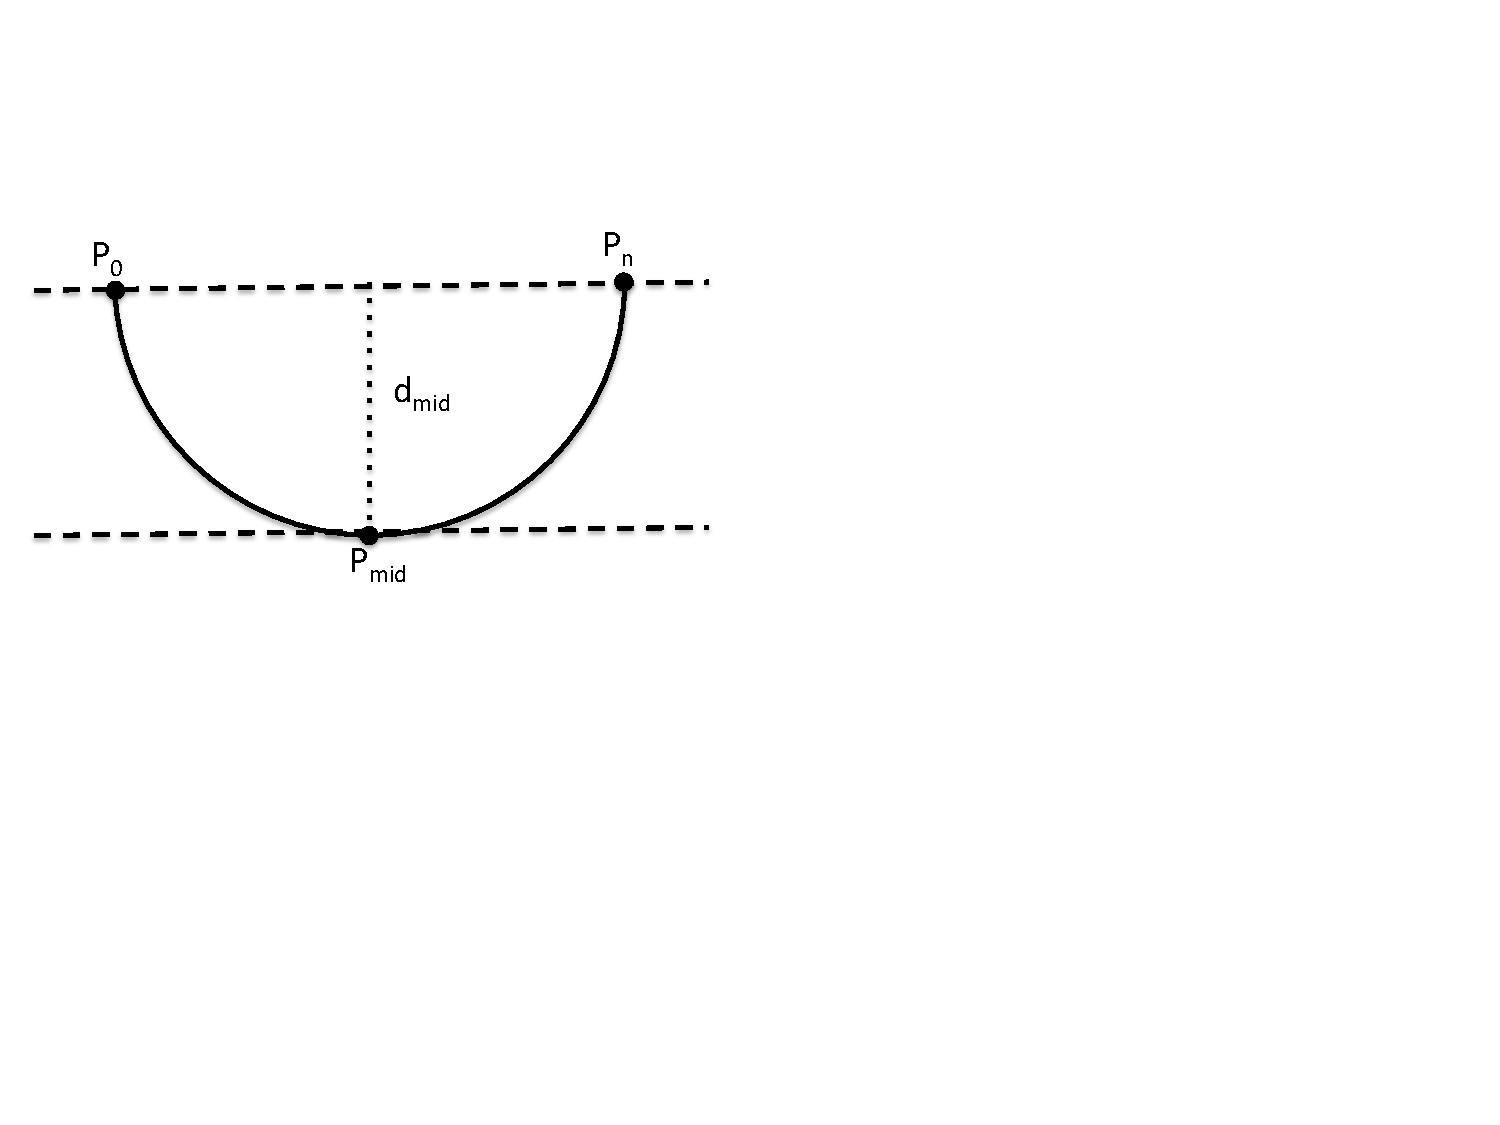
\includegraphics[width=\textwidth]{pics/circ1}   
    \caption{Circularity criterion in a perfect circle is: $|P_0P_n|d_{mid}=0.5$}
     \label{fig:circ1}
  \end{minipage}
  \hfill
  \begin{minipage}[b]{0.49\textwidth}
    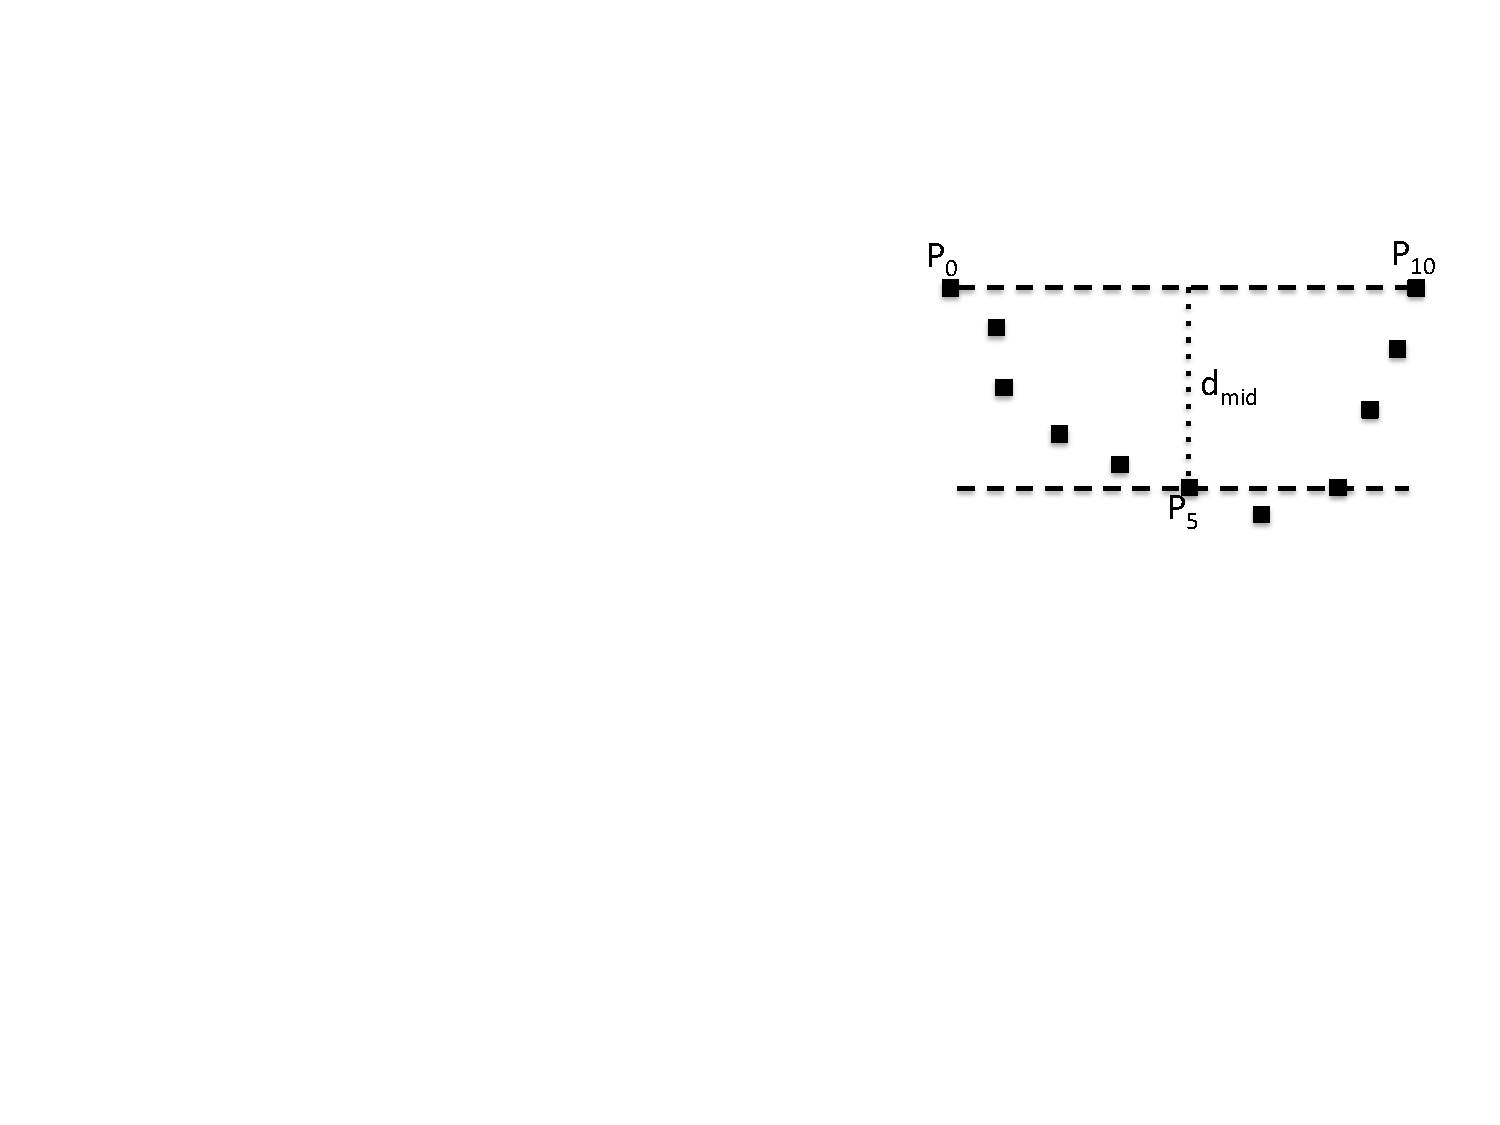
\includegraphics[width=\textwidth]{pics/circ2}    
    \caption{Circularity criterion in a this laser segment is: $|P_0P_{10}|/d_{mid}$}
    \label{fig:circ2}
  \end{minipage}
\end{figure}

\item Inscribed Angle Variance (IAV): This feature is originally proposed by Xavier \cite{xavier2005fast}, in order to detect circles. We adopt IAV in order to detect legs, which are not necessarily circle-shaped, especially for the person-wide blob pattern. As an example, inscribed angles on a circle is shown in Figure \ref{fig:iav}. As a geometric property of the circle, $\angle P_0P_1P_4$ and $\angle P_0P_2P_4$ are equal angles. IAV for a given set of points is the average of all inscribed angles: 
\[
IAV_S = \sum_{P = P_1}^{P_{n-1}} \angle P_0PP_n
\]
For a perfect circle, $IAV_S=90^{\circ}$. For shapes that are not perfect circles but are similar to circles, IAV feature should be consistent. Laser segments from a leg usually resemble a circle, therefore we use IAV as one of the features for leg detection.

\begin{figure}[ht!]
\centering
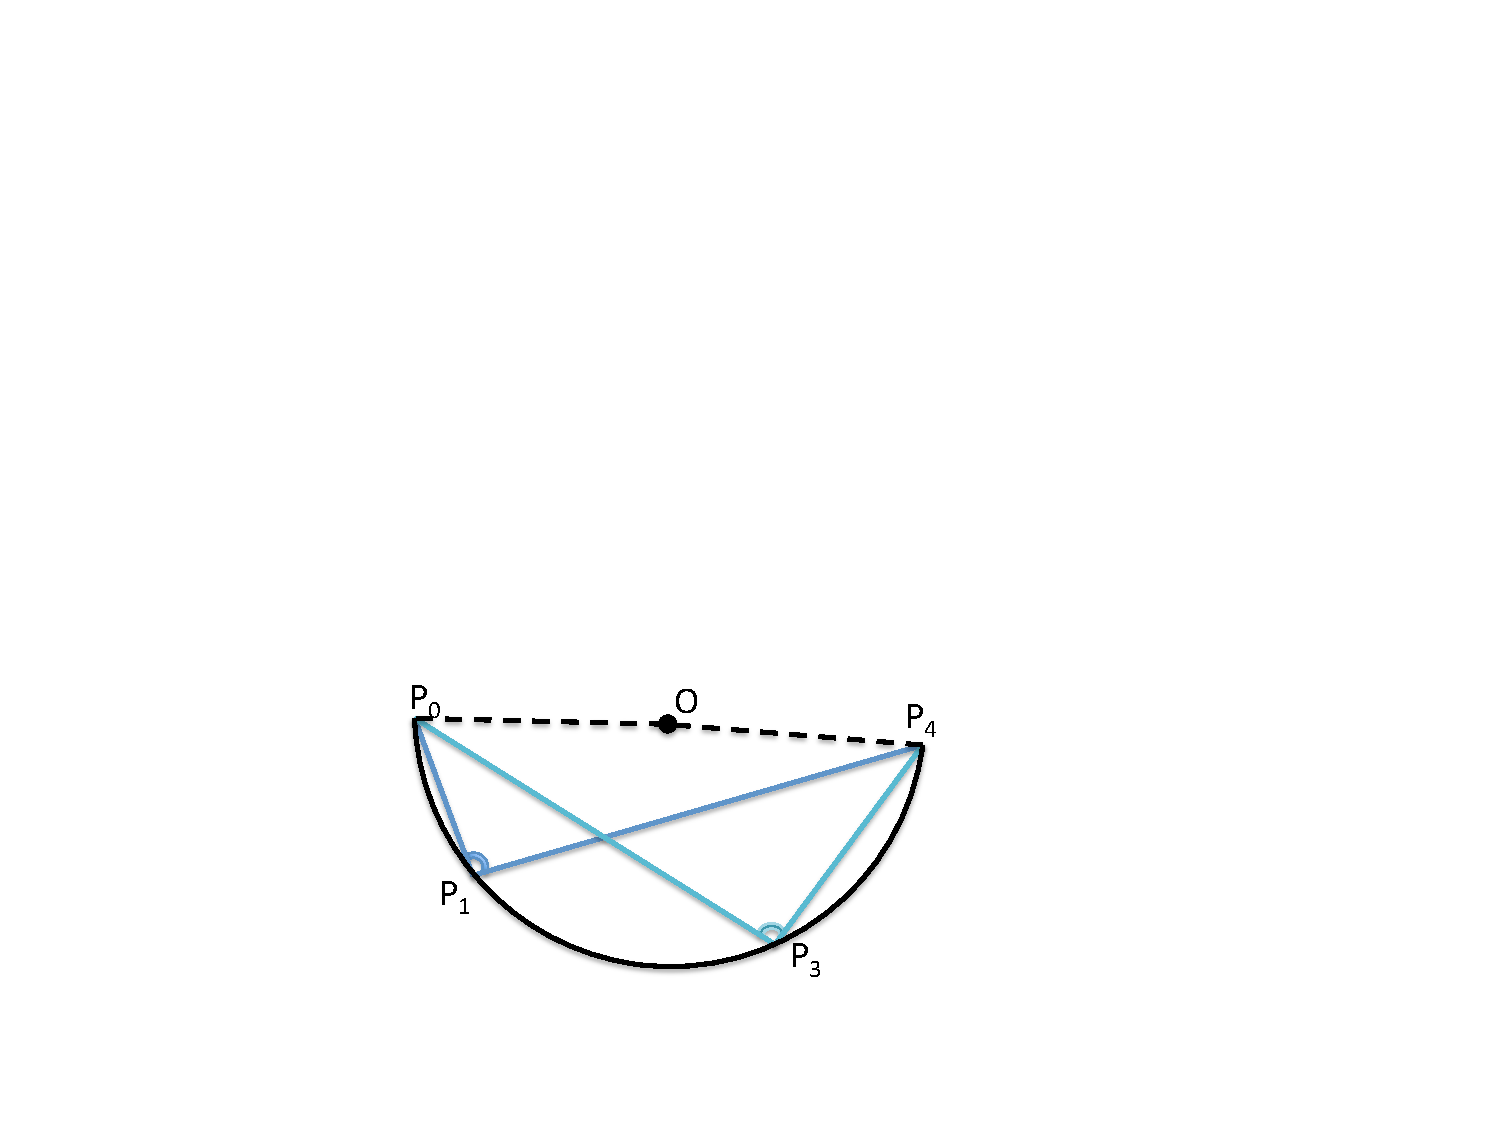
\includegraphics[width=0.4\textwidth]{pics/iav}
\caption{Inscribed angles of an arc are shown in the figure. Inscribed Angle Variance (IAV) is calculated by taking the average of all inscribed angles on a laser segment.}
\label{fig:iav}
\end{figure}

\end{enumerate}

In order to be able to use these values, we first found the nominal feature values for an average human leg. We captured the laser scan data while the robot followed a person through an office environment. The following method used for this experiment will be discussed in detail in Section \ref{sec:following_basic_person_following}. For the training set, two people's legs were recorded with different clothing (shorts, baggy pants and trousers) to account for variance in the leg parameters. About $17\times 10^3$ Single Leg patterns and $0.6\times 10^3$ person-wide blobs were manually labeled in the data. In addition, $120\times 10^3$ segments were labeled as 'other' or 'not a leg'. The average and variance of the aforementioned geometric features for single leg, personwide blob, as well as other segments are given in Table \ref{table:leg_features}. 

\begin{table}
	\centering
  \begin{tabular}{lSSSSSS}    
    \toprule
    \multirow{2}{*}{Segment type} &
      \multicolumn{2}{c}{Width($m$)} &
      \multicolumn{2}{c}{Circularity} &
      \multicolumn{2}{c}{IAV($radians$)} \\
      & {$\mu$} & {$\sigma$} & {$\mu$} & {$\sigma$} & {$\mu$} & {$\sigma$} \\
      \midrule
    Single Leg & 0.13 & 0.03 & 0.25 & 0.15 & 2.23 & 0.4 \\
    Personwide blob & 0.33 & 0.07 & 0.14 & 0.09 & 2.61 & 0.16 \\
    Other & 0.22 & 0.12 & 0.1 & 0.11 & 2.71 & 0.38 \\
    \bottomrule
  \end{tabular}
      \caption{Table shows average and standard deviations of geometric leg features calculated in our dataset.}
    \label{table:leg_features}
\end{table}

For every segment $S_i$ in a test laser scan, we first extract the geometric features $f_1^i,f_2^i,f_3^i$. We then calculate the weighted Mahalanobis distance to the average leg parameters for the each leg pattern:
\begin{align}
\label{eq:mahalanobis}
D_{mah}^i=\sum_{j=1}^{n_{features}} w_j \frac{(f_j^i-\mu_j)^2}{\sigma_j^2}
\end{align}
where $w_j$ are the weights for each feature, $mu_j$ and $sigma_j$ are pulled from Table \ref{table:leg_features}. The resulting Mahalanobis distance is then compared with a detection threshold. If $Dmah_{leg}^{i}< Threshold_{leg}$, the segment $S_i$ is considered a detection. $Threshold_{leg}$ defines how many standard deviations away from the average features are allowed. In our implementation, we empirically set the feature weights as:  $\textbf{W}_{leg} =(0.35, 0.26, 0.39)$, in the feature order given in Table \ref{table:leg_features}. For normal operation, we set  $Threshold_{leg}=1.5$, which accounts for about $\%95$ of the detections. If only one person is being tracked, we use a higher threshold. The reason behind will be explained in Section \ref{sec:multimodal_person_state_estimation}.

\subsubsection{Associating Leg Segments}

After single leg patterns are detected, we try match the leg segments. We extend our leg detection approach to determine which leg segments are connected. Note that this method applies if there is a RGB-D camera pointing to the lower body of the human. For each leg segment pair, if both of them are within the FOV of the RGB-D sensor, we use our algorithm to determine whether there is a connectivity between two candidate leg segments. If a connectivity is found, then the leg segments pair is qualified to be a leg segment pair representing a person. See Figure \ref{fig:leg_connectivity} as an example result. Figure \ref{fig:leg_connectivity_diagram} shows the flow chart of the association algorithm.

\begin{figure}[ht!]
\centering
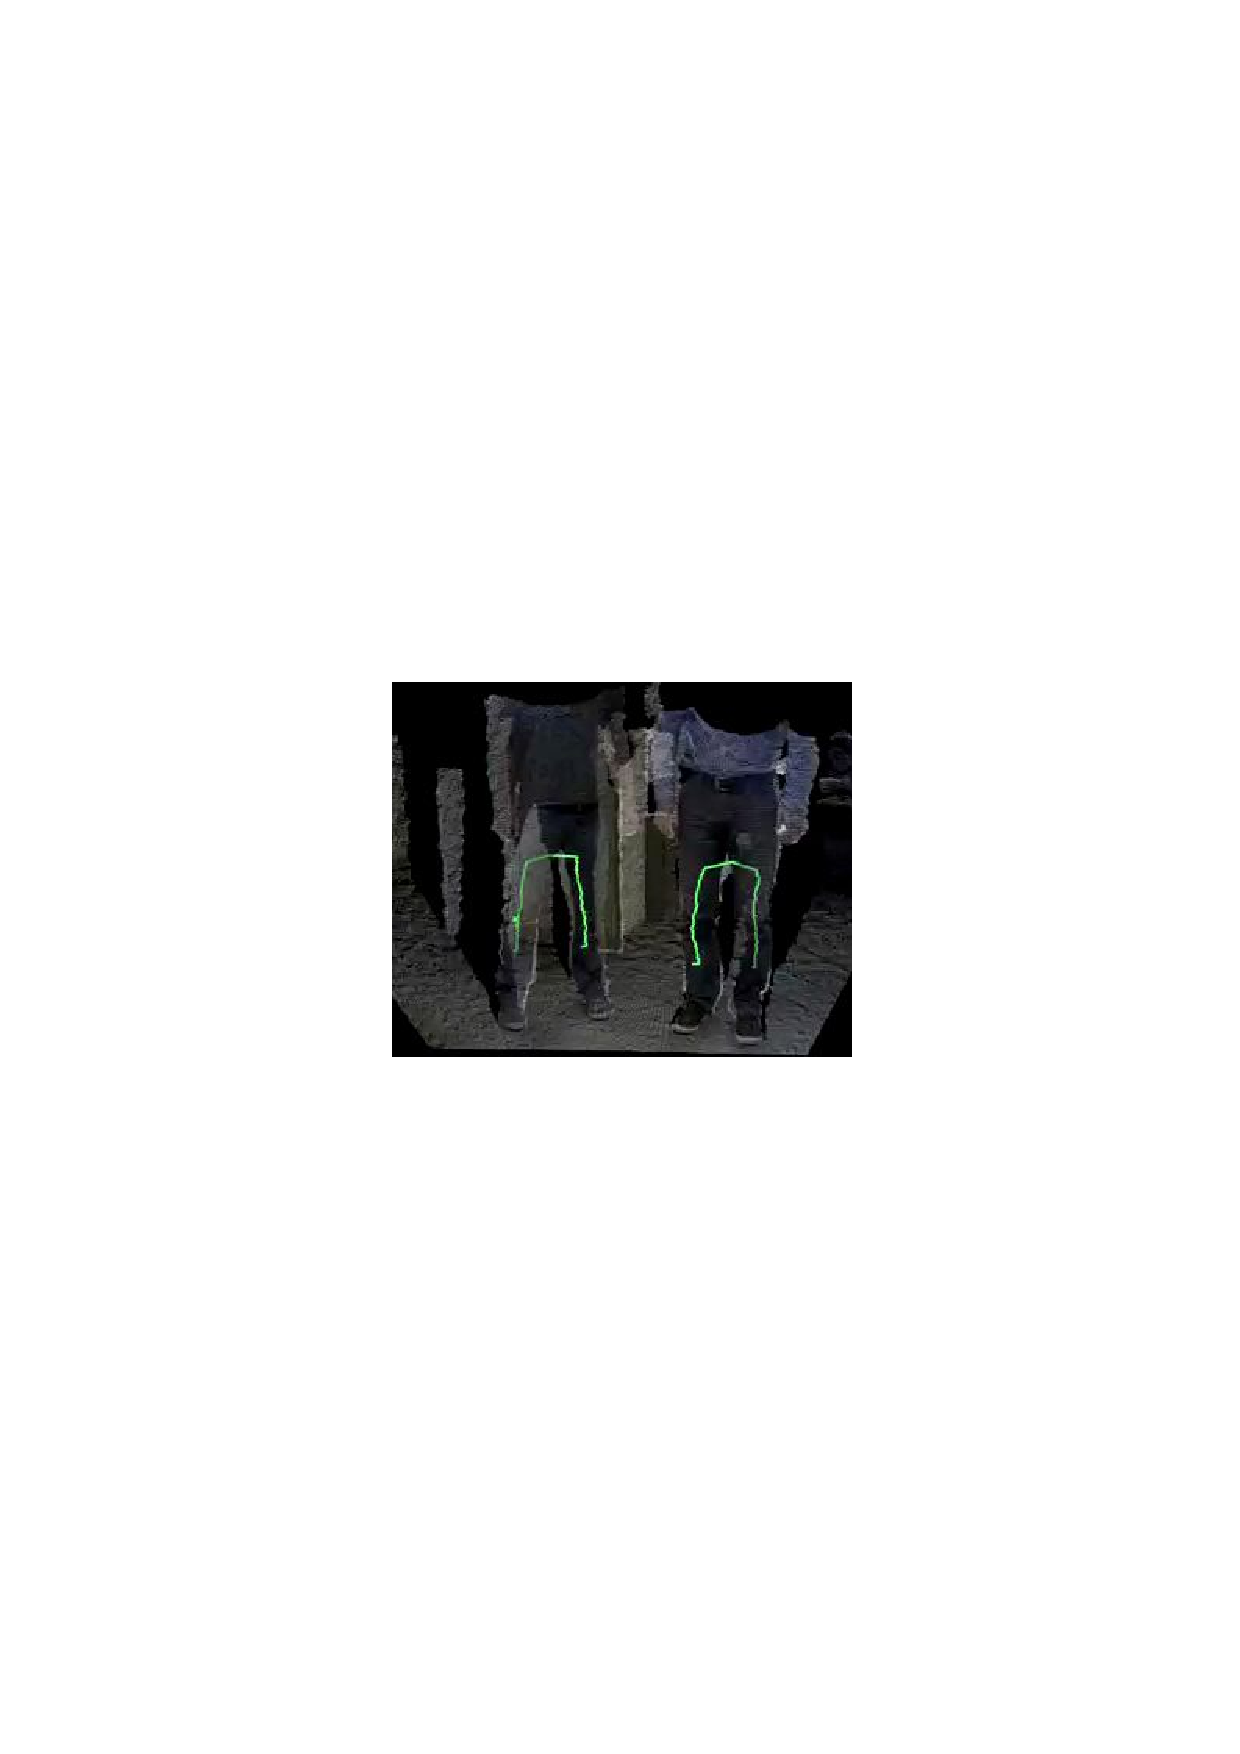
\includegraphics[width=0.6\textwidth]{pics/leg_connectivity}
\caption{Two person detections are seen in this figure. Our leg segment association algorithm propagates pixels vertically from candidate leg segments and connects leg pairs.}
\label{fig:leg_connectivity}
\end{figure}

\begin{figure}[ht!]
\centering
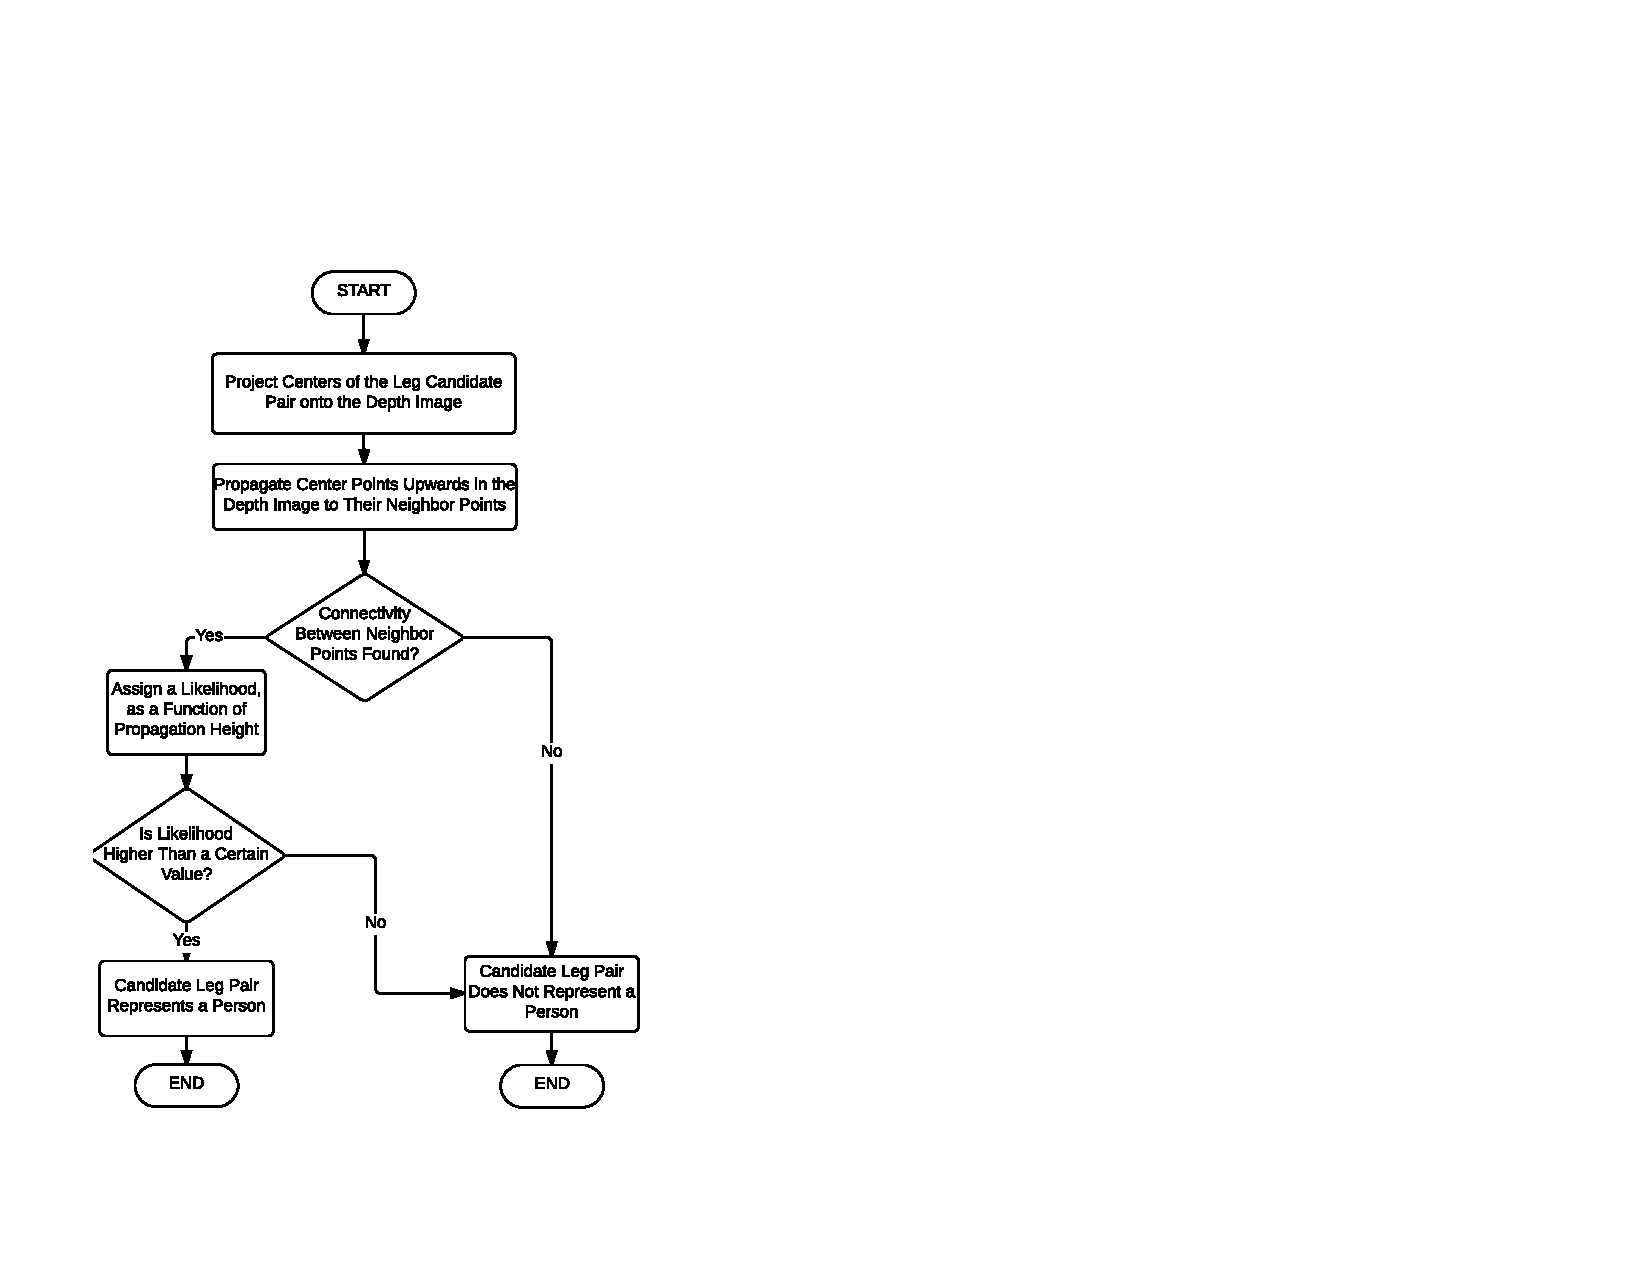
\includegraphics[width=0.5\textwidth]{pics/leg_connectivity_diagram}
\caption{Flow chart for determining if two leg segment candidates belong to a person.}
\label{fig:leg_connectivity_diagram}
\end{figure}

First, the centroids each of the two candidate leg segments are found.  These points are projected onto the depth image acquired from the RGB-D camera. At each iteration, each leg segment, our algorithm first propagates horizontally to both directions in the depth image, then the center pixel is located and it propagates 1 pixel vertically ($+z$ direction). If there are no connectivity after a number of iterations, then we conclude that the candidate leg pair does not represent a person. If there is a connectivity at some point, we then assign a likelihood score to the pair as a function of the vertical propagation height. If this score is higher than a threshold, then the algorithm concludes that the leg candidate segments represent a person. The propagation scoring eliminates most of the false positives due to sensor noise and non-human shapes.

\subsection{Torso Detection}
\label{sec:multimodal_torso_detection}

In this section, we describe our torso detection approach. For this detector, we used another Hokuyo UTM 30-LX laser scanner, placed at torso height ($1.27m$). Our approach relies on fitting an ellipse to laser segments and determining the detection result by interpreting the axis lengths (Figure \ref{fig:ellipse}). Our torso detector allows us to detect the orientation of the person unlike the laser-based leg detectors, therefore this detector is also suitable for applications that relies on extracting the orientation of the person from a single laser scan. 

\begin{figure}[ht!]
\centering
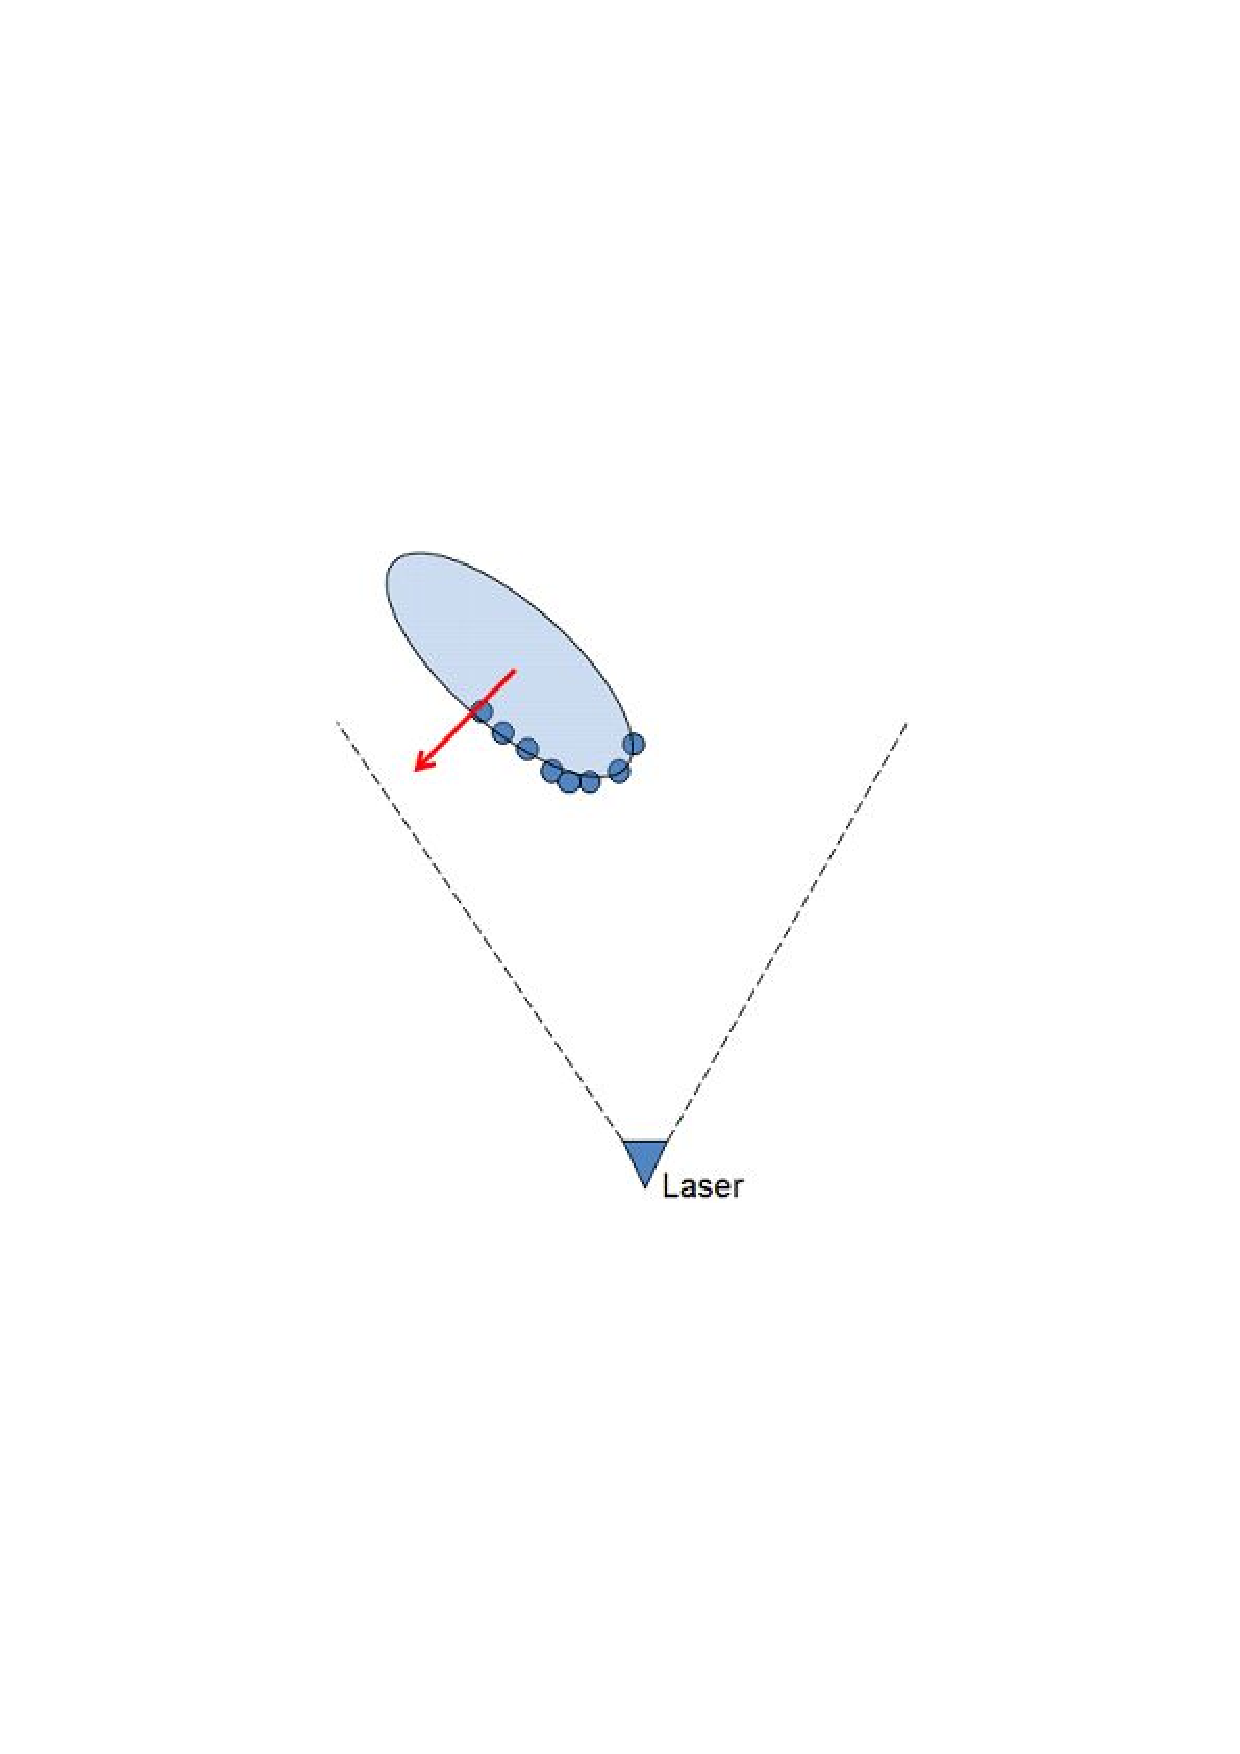
\includegraphics[width=0.35\textwidth]{pics/ellipse}
\caption{Our torso detector fits and ellipse to the human torso and estimate its position and orientation.}
\label{fig:ellipse}
\end{figure}

The first step to detect torsos in a laser scan is to segment the laser scan. We use the same segmentation technique used for leg detection, explained in Section \ref{sec:multimodal_leg_detection}. We then fit an ellipse to each laser segment. We use a numerical ellipse fitting method that solves the problem with a generalized eigensystem, introduced Fitzgibbon \cite{fitzgibbon1999direct}. This ellipse fitting method is robust, efficient and ellipse-specific, so that even very noisy sensor data will always return an ellipse. Compared to iterative methods, it is computationally very efficient, therefore the speed of the calculations is limited to the laser scan refresh rate.

The ellipse fitting algorithm provides us with the centroid and orientation of the ellipse as well as the minor and major axis lengths. To disambiguate the front/back of a person, we assume that people are facing the sensor when they are first detected. While this is a significant limitation our current system, one can potentially utilize face detection as will be described in Section \ref{sec:multimodal_face_recognition} to estimate if the person is facing towards the robot or not.

To detect a torso in a laser segment, we use the minor and major axis lengths, as well as the three geometric features introduced in Section \ref{sec:multimodal_leg_detection}. We collected 450 laser scans in total while a person stood in front of the sensor and made a one full turn around himself. We calculated the mean and standard deviation of the all five features, which is given in Table \ref{table:torso_tracking_results}. For a given laser segment, we find the weighted Mahalanobis distance in Equation \ref{eq:mahalanobis} to the averaged parameters. If $Dmah_{torso}^{i}< Threshold_{torso}$, the segment is considered a detection. The feature weight constants we used was $\textbf{W}_{torso} =(0.19, 0.09, 0.35, 0.24, 0.13)$, in respective order given in Table \ref{table:torso_feature_averages}. These values were empirically determined, although one can do more sophisticated analysis for optimal weights.

\begin{table}
	\centering
  \begin{tabular}{lSSSSSS}    
    \toprule
    {Torso Features}
      & {$\mu$} & {$\sigma$} \\
      \midrule
    Width($m$) & 0.44 & 0.12 \\
    Circularity & 0.32 & 0.18 \\
    IAV($radians$) & 2.57 & 0.38\\
    Major axis length($m$) & 0.39 & 0.08\\
    Minor axis length($m$) & 0.17 & 0.06\\
    \bottomrule
  \end{tabular}
      \caption{Table shows average and standard deviations of geometric features for a human torso in laser scans.}
    \label{table:torso_feature_averages}
\end{table}

Figure \ref{fig:torso_detection_rate} shows how the torso detection rate changes for a given Mahalanobis Distance Threshold in our dataset. What is not displayed in the plot is that higher torso detection rate also means higher rates of false positives. For normal operation, we set $Threshold_{torso}=1.25$, which accounts for about $\%90$ detection rate. If the tracker is dedicated to track only a single person, then we use a higher threshold: $Threshold_{torso}=2.5$. The reasoning behind this threshold selection will be discussed in Section \ref{sec:multimodal_person_state_estimation}.


\begin{figure}[ht!]
\centering
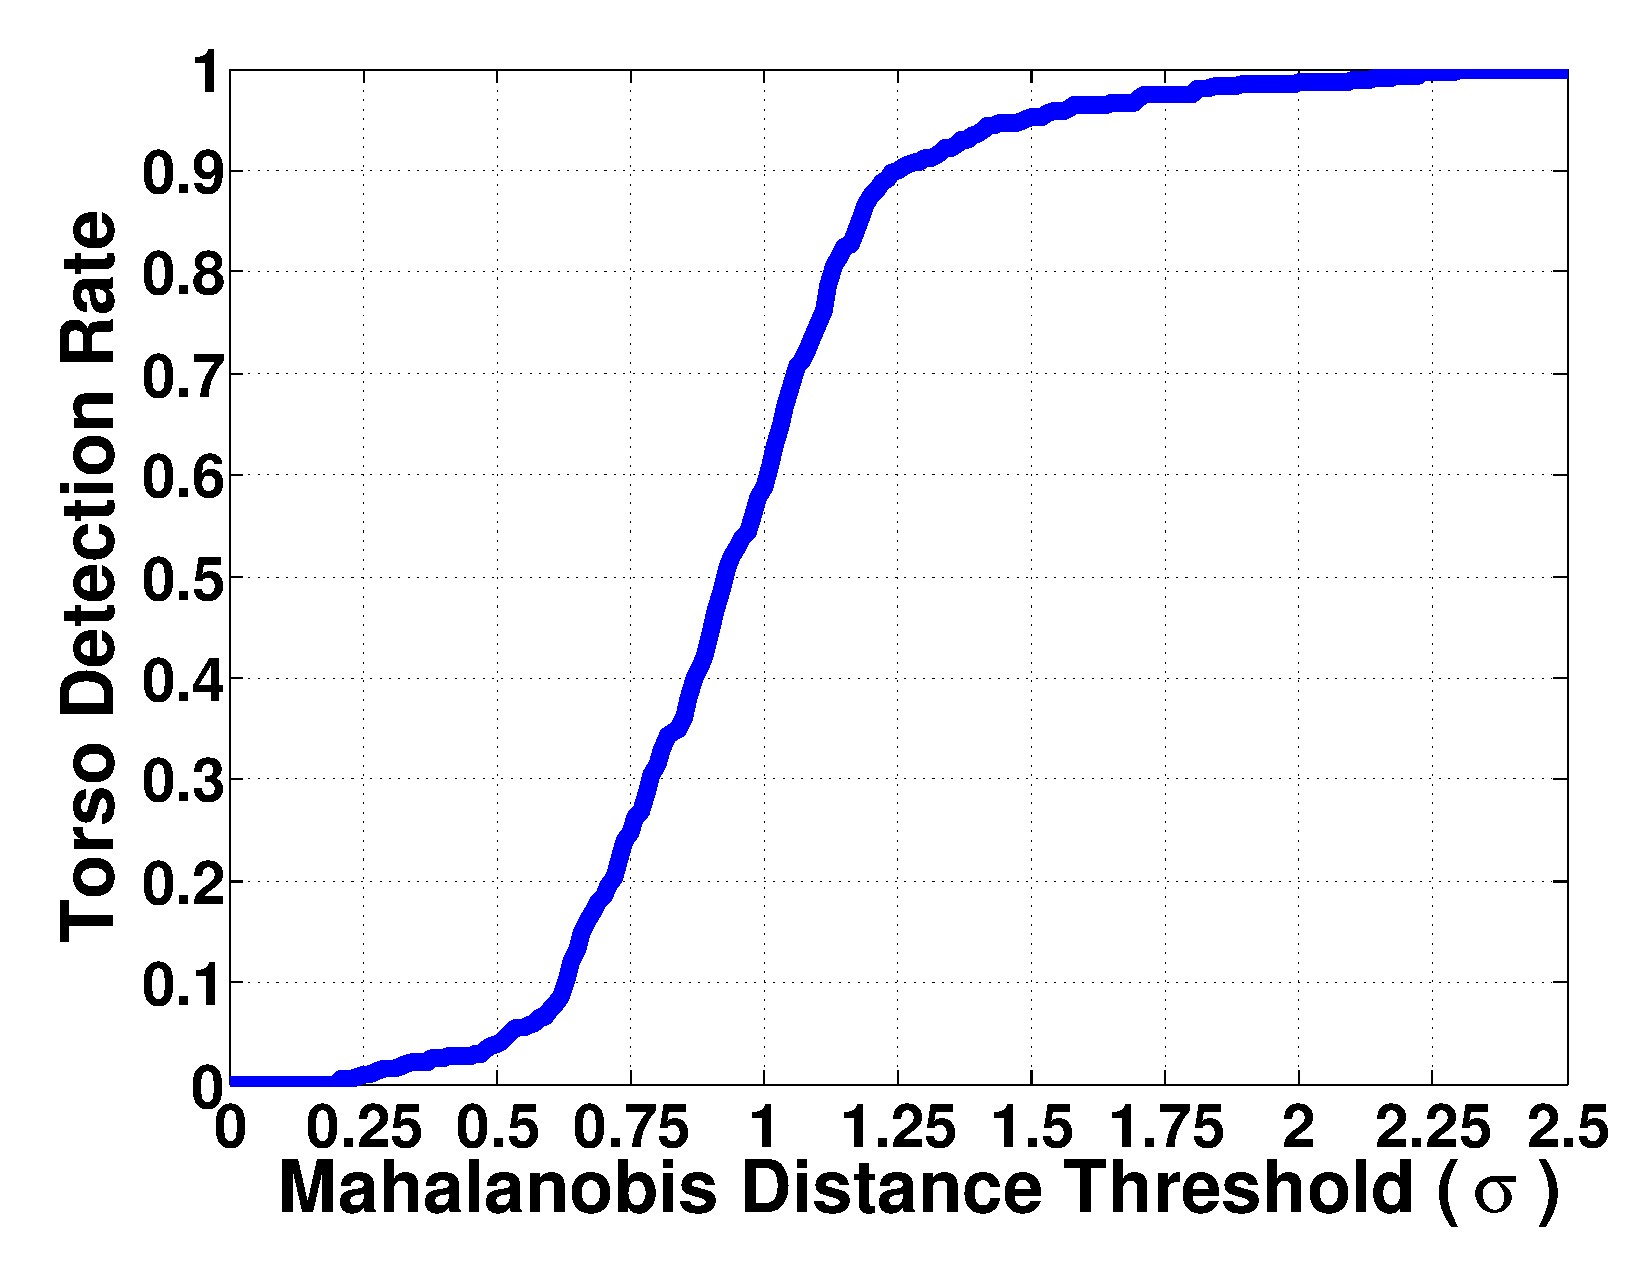
\includegraphics[width=0.6\textwidth]{pics/torso_detection_rate}
\caption{Torso detection rate vs weighed Mahalanobis Distance Threshold in our dataset}
\label{fig:torso_detection_rate}
\end{figure}

\subsubsection{Evaluation of Torso Detection}

In order to evaluate the accuracy of the position and orientation estimations of our torso detection method, we collected torso data from 23 people. Subjects were instructed to stand on 4 targets at different distances with 8 different orientations on each target. Experimental setup from the sensor's view is shown in Figure~\ref{fig:torso_tracking_exp_setup}. For each pose at every target, we logged the position and orientation estimation of the torso detector and compared it with ground truth, which is fixed.

\begin{figure}[h]
\centering
        \subfigure{%
            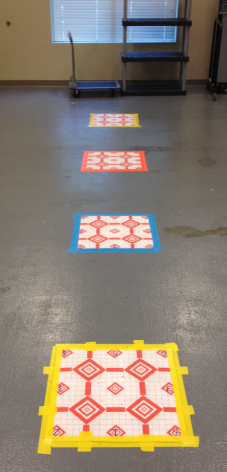
\includegraphics[width=0.2\textwidth]{pics/exp0}
        }%
        \subfigure{%
            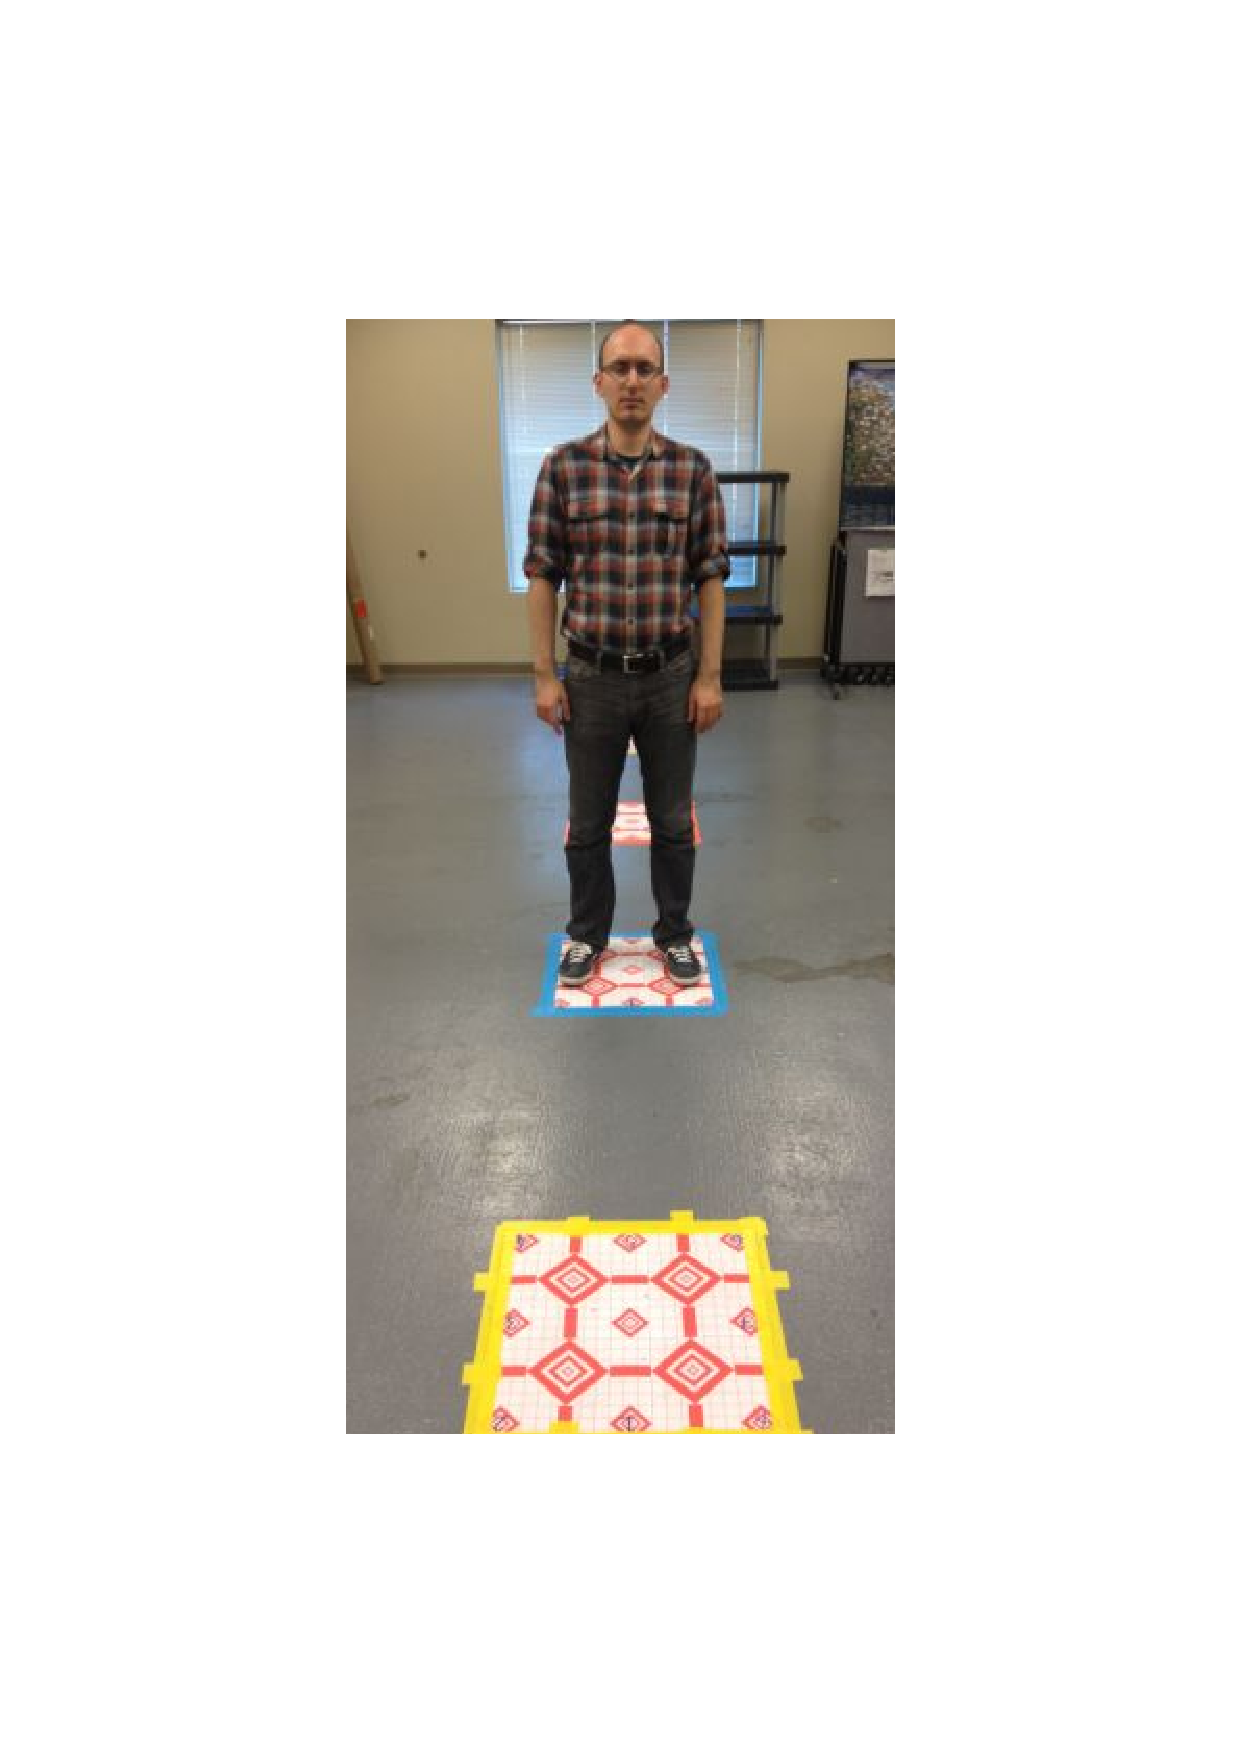
\includegraphics[width=0.211\textwidth]{pics/exp1}
        }%
        \subfigure{%
           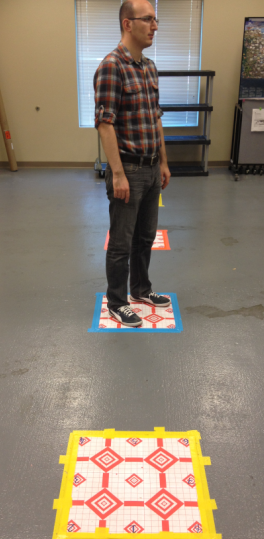
\includegraphics[width=0.205\textwidth]{pics/exp2}
        } %  ------- End of the first row ----------------------%
        \subfigure{%
           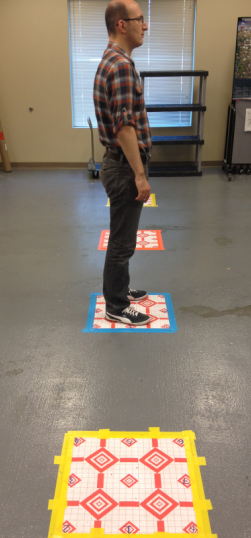
\includegraphics[width=0.197\textwidth]{pics/exp3}
        }\\ %  ------- End of the first row ----------------------%
    \caption{%
	Experimental setup for the evaluation study of the Torso Detector.
     }%
   \label{fig:torso_tracking_exp_setup}
\end{figure}


Table~\ref{table:torso_tracking_results} shows the angular error at every target distance and human orientation with respect to the laser scanner. 

\begin{table}[ht!]
\centering
\begin{tabular}{cSSSSSSSSS}    
 \toprule 
Distance To Laser & {N} & {NE} & {E} & {SE} & {S} & {SW} & {W} & {NW} & {ALL}\\
\midrule
{$1.0m$} & {$4^{\circ}$} & {$12^{\circ}$} & {$22^{\circ}$} & {$13^{\circ}$} & {$5^{\circ}$} & {$7^{\circ}$} & {$26^{\circ}$} & {$17^{\circ}$} & {$13^{\circ}$} \\
{$2.5m$} & {$5^{\circ}$} & {$16^{\circ}$} & {$19^{\circ}$} & {$10^{\circ}$} & {$3^{\circ}$} & {$6^{\circ}$} & {$14^{\circ}$} & {$17^{\circ}$} & {$11^{\circ}$} \\ 

{$4.0m$} & {$4^{\circ}$} & {$10^{\circ}$} & {$30^{\circ}$} & {$16^{\circ}$} & {$7^{\circ}$} & {$11^{\circ}$} & {$21^{\circ}$} & {$17^{\circ}$} & {$15^{\circ}$} \\ 
{$5.5m$} & {$5^{\circ}$} & {$11^{\circ}$} & {$41^{\circ}$} & {$18^{\circ}$} & {$10^{\circ}$} & {$6^{\circ}$} & {$38^{\circ}$} & {$23^{\circ}$} & {$19^{\circ}$} \\ 

{ALL} & {$4^{\circ}$} & {$12^{\circ}$} & {$27^{\circ}$} & {$14^{\circ}$} & {$6^{\circ}$} & {$7^{\circ}$} & {$24^{\circ}$} & {$18^{\circ}$} & {$14.5^{\circ}$} \\
\bottomrule
\end{tabular}
\caption{Average orientation error of the torso detector with respect to distance from sensor and body pose in a study with 23 people}
\label{table:torso_tracking_results}
\end{table}

The average positional error was about $5cm$ regardless of the distance and the orientation of the human. The average orientation error throughout all the experiments was $14.5^{\circ}$. Error in orientation, however, varied greatly by pose of the person with respect to the laser scanner. Average error in orientation differed slightly with respect to the distance from the sensor and was the least with $11^{\circ}$ when the humans were $2.5m$ away from the sensor. We attribute to the fact that when humans closer than $2.5m$ to the laser scanner, it captures more of the arms, which makes the fitted ellipse slightly worse. The orientation of the human with respect to the sensor had a significant effect on orientation error. Least error was achieved when people faced the sensor  ($4^{\circ}$) or the opposite way ($6^{\circ}$). On the other hand, average orientation error was $24^{\circ}-27^{\circ}$ when humans are perpendicular to the sensor, because a large portion of the torso is not visible to the laser scanner in that configuration.

\section{Person State Estimation}
\label{sec:multimodal_person_state_estimation}

The position and velocity of the person can not be determined by direct observation due to measurement noise and false detections. Therefore there is a need for a filtering algorithm in order to estimate the state of a person. Using a state predictor for human movement has two advantages. First, the predicted trajectories are smoother than raw detections. Smooth tracking helps the robot maintain consistent trajectories for high-level applications such as Person Following (Section \ref{chapter:person_following}). Second, it provides a posterior estimation that can be used for data association when there is a lack of matching detections. This allows the tracker to handle temporary occlusions. We use a discrete Kalman Filter \cite{kalman1960new} to predict the position of a person. There are other types of filtering techniques available in the literature, such as Particle Filters \cite{khan2004mcmc}. Since the results of the person state estimator is used by time-critical higher level applications, the tracker should come up with an estimate in real time. Therefore the choice of using Kalman Filters was motivated by its computational efficiency. Efficient person state estimation also increases the safety of the robot, as the robot can react faster if there are people in close proximity.

Accoding to Hicheur \cite{hicheur2005velocity}, humans tend to maintain a constant speed when they are walking straight and reduce speed while turning. We used constant velocity model which assumes people will maintain their speed. Even though this assumption is not always true, it provides a simple model without sacrificing too much from tracking performance.

The Kalman filter estimates a process as a predictor-corrector cycle using feedback control. The process has two cycling states: time update and measurement update as shown in Figure. Time update projects the state forward by using the current state and error covariance. Measurement update is responsible for the feedback and corrects the previous estimate.

The Kalman Filter is governed by two linear stochastic difference equations:
\begin{align}
s_k&=As_{k-1}+Bu_{k-1}+w \\
z_k&=Hs_k+v
\end{align}

Where $s_k$ represents the process state at time step $k$, $A$ is the state propagation matrix, $B$ relates the optional control input $u$, $z_k$ is a measurement, $H$ is the measurement observation matrix. $w$ and $v$ represent the process and measurement noises, respectively, drawn from normal probability distributions with zero mean $N(0,Q)$ and $N(0,R)$.

We define the state of a person $s_k$ at time step $k$ as:
\begin{align}
s_k & =
\begin{bmatrix} 
 x_k \\ 
 y_k\\
 \dot{x}_{k} \\
 \dot{y}_{k}
\end{bmatrix}
\end{align}

where $(x_k,y_k)$ is the position and $(\dot{x}_{k}, \dot{y}_{k})$ is the velocity of the person in Cartesian Coordinates. With the constant velocity model, the time update equations are:
\begin{align}
x_k&=x_{k-1}+\dot{x}_{k-1} \Delta t_k + w\\
y_k&=y_{k-1}+\dot{y}_{k-1} \Delta t_k + w\\
\dot{x}_{k}&=\dot{x}_{k-1} \\
\dot{y}_{k}&=\dot{y}_{k-1}
\end{align}
resulting in the following Kalman Filter matrices:
\begin{align}
A =
\begin{bmatrix} 
 1 & 0 &\Delta t_k & 0\\
 0 & 1 & 0 & \Delta t_k\\
 0 & 0 & 1 & 0\\
 0 & 0 & 0 & 1
\end{bmatrix} &&
B =
\begin{bmatrix} 
 0 \\
 0 \\
 0 \\
 0
\end{bmatrix} &&
H =
\begin{bmatrix} 
1 & 0 & 0 & 0 \\
 0 & 1 & 0 & 0
\end{bmatrix} 
\end{align}
where $\Delta t_k$ is the time difference from the previous detection. A track is lost if there are no detections for a fixed amount of time. At every time update of a filter, if $\Delta t_k$ is larger than a fixed threshold, the track is killed.

The reason $B$ vector is zero is that we track people in the world frame and robot motion is already accounted for with robot localization. For this reason, we assume there are no control inputs to our system. The noise matrices we used are:
\begin{align}
Q=qI_4
&&
R=rI_2
\end{align}

where we used $q=0.02$ and $r=1.0$ in practice.

Our approach is multimodal in the sense that asynchronous measurements are accepted from different sources as long as they provide a positional estimate in the respective sensor frames. Using the latest localization information, this position is converted to the world frame and then fed as a measurement to the active filters. We apply an additional layer of filtering to every detection before it is considered a measurement. We check if a new detection is in collision with the static map, and it if is in collision, we reject that particular detection. The check against the static map is fast and helps reduce false positives in practice. We use Nearest Neighbor (NN) data association \cite{bar1995multitarget}, which is a reasonable compromise between performance and computational cost. 


Depending on the task, a single person or multiple people must be tracked. We examine each case below:

\begin{itemize}
\item \textbf{Single target tracking:} For some tasks, such as person following, dedicated tracking of a single specific user is required and tracking bystanders is not required for task success. In this case, our goal is to keep tracking the specific user, so we significantly relax the detection thresholds of the detectors. Even though doing so results in more spurious detections, we do not start more than a single track. This approach improves the tracking performance of a single person.
\item \textbf{Multi-target tracking:} When the robot is navigating to a goal point with human bystanders, tracking multiple people at the same time is necessary. Moreover, losing track of a bystander would not be very detrimental to task success. We keep a separate Kalman filter for each tracked person. If a detection is matched to multiple filters, only the closest filter is associated with the detection and the other filters are considered to have no detections for that time step.
\end{itemize}




 




\section{Face Recognition}
\label{sec:multimodal_face_recognition}

For certain interactive navigation tasks such as finding a specific person, a robot needs to have person recognition capability. Our person recognition approach uses face recognition and optionally shirt color features. We detect faces in RGB images using the popular face detector by Viola and Jones \cite{viola2004robust}. We use the Eigenface method by Turk and Penland \cite{turk1991face} for face recognition. Our approach allows new faces to be trained on-the-fly.

With the $Eigenface$ approach, face are represented in a lower-dimensional space. Sirovich and Kirby \cite{sirovich1987low} showed that dimension reduction method Principal Component Analysis (PCA) can be used on face images to form a set of basis features. The main idea of PCA for faces is to find vectors that best account for variation of face images in all training images. These vectors are called $eigenvectors$. Then a face space is constructed called $eigenfaces$ and the images are projected onto this space. Our approach of face recognition works as follows:

\begin{figure}[ht!]
\centering
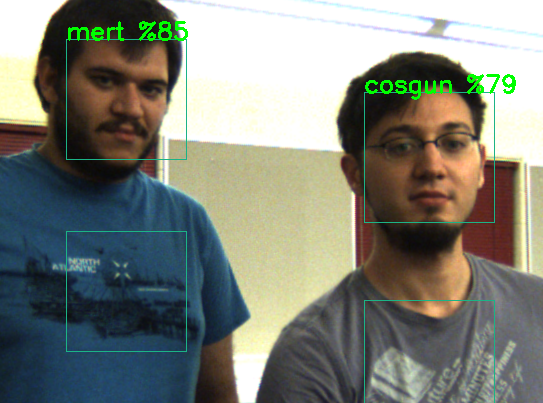
\includegraphics[width=0.6\textwidth]{pics/person_recognition}
\caption{Example results of our person recognition method is shown in the image. We use $Eigenfaces$ face recognition method and optionally shirt color recognition.}
\label{fig:person_recognition}
\end{figure}

\begin{enumerate}
\item A person unknown to the system comes up to the robot and initiates training.
\item Robot asks the person to turn his face one side to another, and takes M face and shirt images of this person.
\item Eigenfaces from the entire training set is calculated, and every known face is projected to the corresponding M-dimensional weight $facespace$.
\item After training is completed, face recognition is reactivated.
\item A distance value from face recognition and optionally from shirt color recognition is received and it is thresholded for a decision. An example recognition result is in Figure \ref{fig:person_recognition}. 
\end{enumerate}

Using the UI of the robot, a user can start training and adjust the information in the person database. The person data is managed by a SQLite database hosted locally on the robot.

Shirt color recognizer can be used when there is little time between the training and recognition. Activating the shirt recognition should improve recognition and reduce false positive detections. We assume a rectangular region below the face captures the shirt ($1.5$ times below the the face rectangle size). The distribute the histogram into bins using normalized RGB color space because of its relative robustness to lighting. For detection, we calculate the distance between the training histogram to the test histogram using Earth Mover Distance \cite{rubner1998metric}. The color histogram is adaptively updated at every high confidence detection in order to account for illumination changes. The overall person score is calculated by a weighted average of face and shirt distance.

%A possible use of person recognition in interactive navigation is to drive up to a specific person. Another possible use case for our work is to re-initialize person following if the user is lost. We have used face recognition in some of our applications, however it requires the face of the person to be visible. Vision community works on datasets that are selected nicely as pictures taken by humans are likely to have more faces in it. On the other hand, most frames the robot acquires won't have any faces in it. Development of person recognition approaches that are suited for on-board sensing on mobile systems is an open research area.
%%%%%%%%%%%%%%%%%%%%%%

\chapter{Person Following}
\label{chapter:person_following}

In this chapter, we focus on one aspect of human-robot interaction, namely person following in an indoor environment. There are many scenarios in which a person following robot can be useful. For example, a robot can carry luggage of travelers in airports, or groceries in a supermarket. Person following is also the enabling capability for interactive acquisition of the \textit{Home Tour} scenario discussed in TODO. The robot needs to know how to follow a person before building an environment representation and providing services to the user.  There are two properties a person following behavior should achieve: robust following and social awareness. 

Typically, a service robot operates in a dynamic and populated environment, therefore the robot must be able to keep track of a single person even when they are temporarily occluded. Multimodal person tracking that is presented helps the robot to have better estimates of a user's position. As discussed in Chapter \ref{chapter:multimodal_person_detection_and_tracking}, for the person following task, the robot has to track a designated user, and the detection thresholds of detectors are relaxed for robust tracking at the expense of more false positive detections. 

The robot not only has to keep appropriate distance to the user, but it also has to recognize $what$ the user is trying to accomplish and move accordingly. For example, during the home tour scenario, when the user stops, the robot should predict that the user is going to annotate a landmark, and it should come beside the user instead of standing behind. Moreover, the robot should be smarter when passing doors or following a person who is cutting a corner. In order to be able to handle these scenarios, the robot should act beyond purely reactive following behavior. It is desirable for the robot to anticipate what action the user is likely going to take and act accordingly.

In this chapter, after referring to previous studies on person following robots in Section \ref{sec:following_related_work}, we present the elementary person following method in \ref{sec:following_basic_person_following}. After that, in Section \ref{sec:following_situation_aware} we demonstrate situation awareness of a person following robot in three commonly encountered scenarios: door passing, user activity awareness and handling corners. In Section \ref{sec:following_application_to_telepresence}, we present an application of person following to telepresence robots.

\section{Related Work}
\label{sec:following_related_work}

A robot that follows a person is a widely studied scenario in robotics. A relevant body of work is pursuit evasion \cite{chung2011search}, however the target is trying to evade the follower. In person following robots, we assume that the target is cooperating with the follower.

In one of the earliest works in this area by Sidenbladh \cite{sidenbladh1999person}, robot keeps the person centered in the camera image using a P controller. Prassler \cite{prassler2001motion} also offers a fully reactive approach using the \textit{Velocity Obstacles} concept, which uses the velocity of the target to find allowable velocities of the robot that guarantees avoiding collision if both the target and the robot move with constant speed. The approach is applied on a wheelchair, even though social constraints were not considered. 
The robot does not necessarily follow a person directly from behind. Gockley \cite{gockley2007developing} observed how people walk together. It is reported that partners who were conversing tend to look forward with occasional glances to each other. Ohya \cite{ohya2002intelligent} presents a following method to escort a target on the side while avoiding obstacles. It was assumed that the target would move with the same acceleration and velocity. Murakami \cite{murakami2014destination} presents a method to first estimate the sub-goal of the leading person and then following as if the robot knows the goal. 

Park \cite{park2013autonomous} models the problem as a control problem and offers an algorithm based on Model Predictive Control.
\cite{miura2010development} employs randomized tree expansion and biases the calculated paths towards a sub-goal, which is the current position of the person. Hoeller \cite{hoeller2007accompanying} adopts the virtual targets idea and selects a goal position in a circular region around the person. Stein \cite{stein2013navigating} proposes choosing and following a leader to handle navigation in crowds.

Some of the relevant works considered the social side of the interaction. Gockley compared two elementary following methods: direction following, where the robot always attempts to drive towards the tracked person, and path following, where the robot follows the path the person took. It was shown that direction following behavior was perceived as more human-like and natural than path following. Yuan's \cite{yuan2008spatial} system switches following behavior between parallel following, direction and path following depending on the layout of the obstacles. Zender \cite{zender2007human} emphasizes on situation awareness for following and studies cases of handling doors and corridors. To handle the doors, the robot increases its following distance and that leads the robot to wait for a while. Following in a corridor is handled with an approach similar to Pacchierotti \cite{pacchierotti2005human}, and the robot's speed is increased. \cite{loper2009mobile} presents a system that is capable of responding to verbal and non-verbal gestures and follow a person. When following a group of people, a common method is to choose and follow a leader. Granata \cite{granata2012framework} presents behaviors such as going towards, following and searching a user. Ota \cite{ota2013recovery} touches upon the recovery functions whenever the robot loses tracks of the leading person.

\section{Basic Person Following}
\label{sec:following_basic_person_following}

In this section, we describe our basic person following method. To keep track of the person

When the following behavior is initiated from a higher level process, first the person to be followed must be tracked. The robot looks for the closest person in the vicinity of the robot (within $2m$). If no person is detected for some time, then the command is invalidated. We use the person detection and tracking system described in Section \ref{chapter:multimodal_person_detection_and_tracking}.

\begin{figure}[ht!]
\hspace*{4cm} 
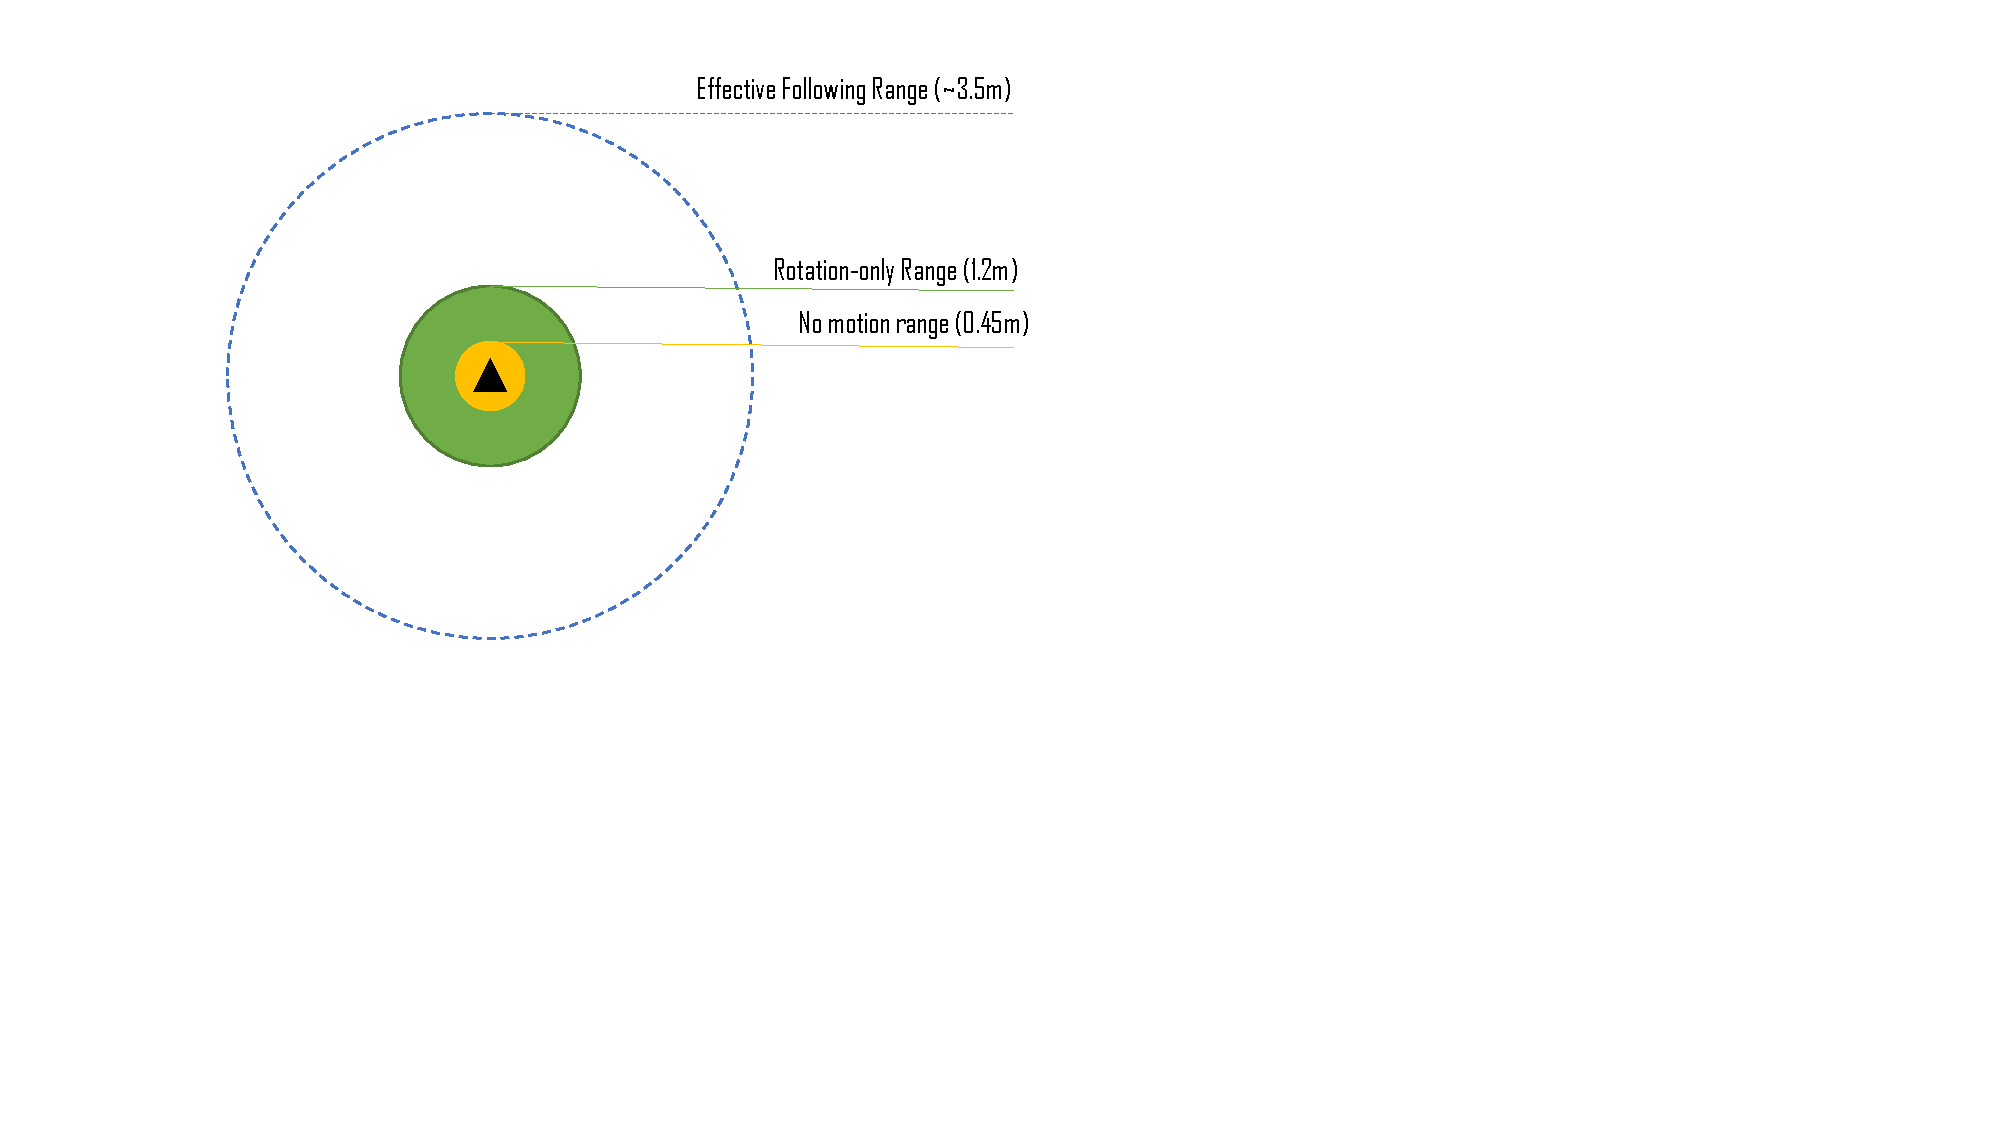
\includegraphics[width=0.7\textwidth]{pics/following_ranges_cropped}
\caption{Overhead view of relevant ranges for person following. Robot is represented as the triangle in the middle.}
\label{fig:following_ranges}
\end{figure}

In the basic person following mode, the robot has three different strategies depending on the distance towards the followed person. The distance to the user is calculated as the distance from the center of the robot base to the person's current location estimation. We used Hall's characterization of personal spaces in order to determine the distance limits. See Section TODO for a review of Hall's work. The three distinct zones and corresponding robot behavior are given as follows:

\textbf{Intimate Zone $[0-0.45m]$:} In this short interval, the person is very close to the robot, therefore any motion of the robot may be potentially unsafe. Therefore the robot comes to a complete halt in this zone ($v=0,w=0$). This behavior also allows the user to safely interact with the on-board User Interface.

\textbf{Personal Zone $[0.45-1.2m]$:} When the robot is in the personal zone of the user, the robot stops and only rotates towards the followed person ($v=0,w=w_{rotation}$). The rotational velocity is determined with a P controller, with the error term defined as the difference between the current orientation and the tracked person's orientation. The rotational velocity is capped at a fixed value, so that the person feels comfortable with the rotation of the robot.

\begin{figure}[h!]
\centering
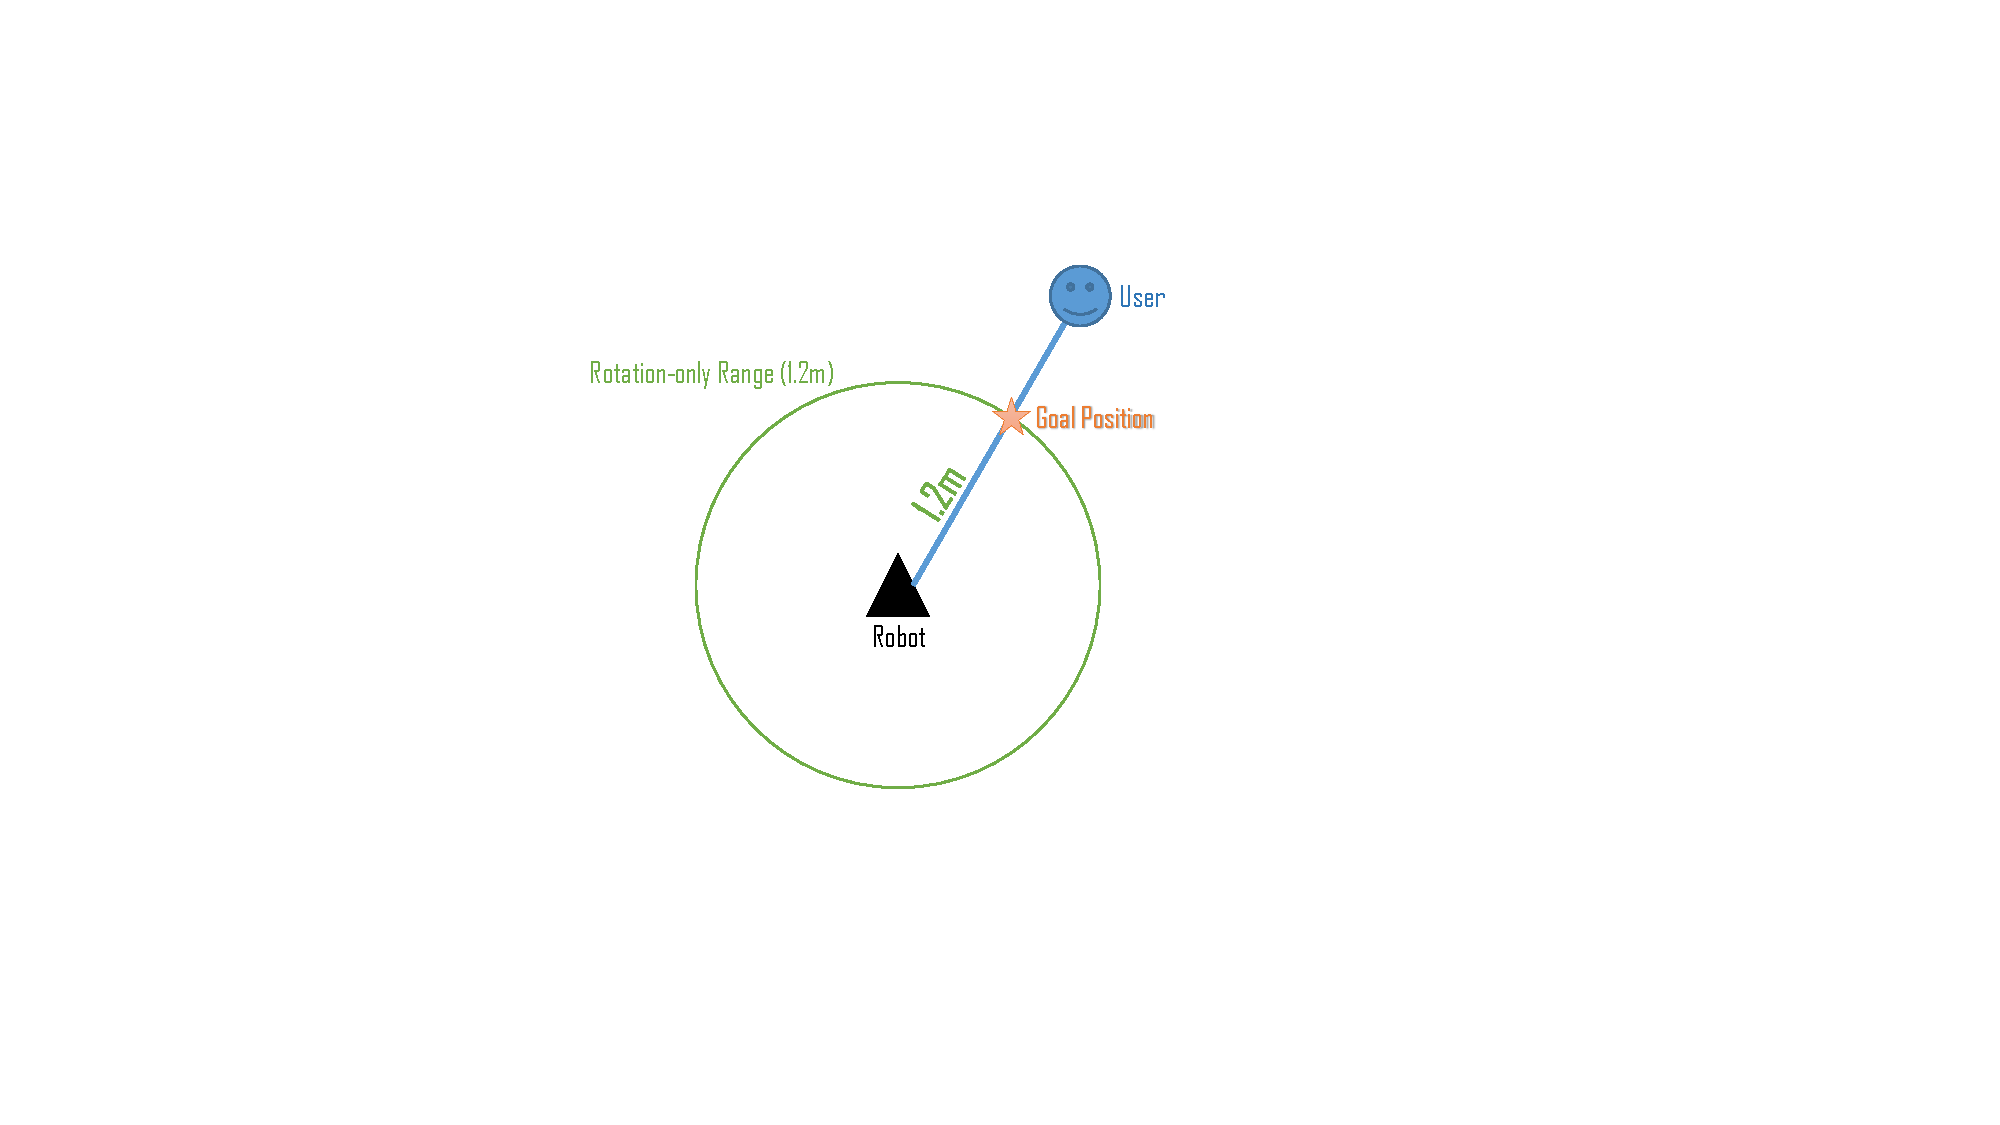
\includegraphics[width=0.55\textwidth]{pics/following_1m_cropped}
\caption{An illustration of how the goal position is calculated when the user is in the social space $[1.2m-3.5m]$.}
\label{fig:following_1m}
\end{figure}

\textbf{Social Zone $[1.2m-3.5m]$: } In this range interval, the robot executes the main following behavior. At every time step, a goal pose that is $1.2m$ away from the and headed towards the user is calculated, see Figure \ref{fig:following_1m} for an illustration. A collision-free path is found and the robot executes this path until a new measurement from the tracked person is received. The path is found using Dynamic Window Approach (DWA) local planing method. We use the ROS implementation of DWA for the basic following behavior.

Sometimes it is inevitable that the person tracking system loses the target, particularly when the person is consistently faster than the robot or the person goes outside the range of the sensors (further than $\sim3.5m$ in our case). When this happens, the robot will attempt to go to its last calculated goal position and look for the person. By this means, the robot attempts to keep up with the lost person as far as possible with the hope that the person will re-appear in the vicinity of the last seen position. After the robot reaches this goal, it stops and waits for an amount of time. If the user is saved to the database, or the robot already knows that he/she is in the database, then the face recognition system described in Section \ref{sec:multimodal_face_recognition} is activated. Otherwise, the robot continues following the closest person that appears in this position. If no person is detected within a fixed amount of time, $5$ seconds in our implementation, then the robot declares that the person is lost.


\section{Situation Aware Person Following}
\label{sec:following_situation_aware}

\subsection{Door Passing}

\subsection{User Activity Awareness}

\subsection{Corners}


\section{Application To Telepresence Robots}
\label{sec:following_application_to_telepresence}

A telepresence robot can be described as \textit{Skype on wheels}, where a remote user teleconferences while having the control of the movement of a robotic system in a physical environment. Telepresence robots constitute a promising area in the consumer robotics industry as evidenced by multiple start-up companies working on telepresence products. However, currently all the telepresence robots that are available in the market are controlled by manual driving - usually via the keyboard or a joystick. In this section, we present an implementation of person following on a telepresence robot and a user study that evaluates effect of having person following capability on a telepresence robot.

Telepresence robots are a level above video conferencing since the robot is used as the communication medium and the remote user can now control the movement. Therefore, the spatial interaction between people and a telepresence robot in social situations is worth investigating. One of those situations is moving with a group of people. In an effort to analyze the spatial and verbal interaction, we focus on engagement with one person where the remote user interacts with the person while following him/her in a corridor. This is situation is very likely to happen in office environments, for example when the remote user is having a discussion with a co-worker while walking to his office after a meeting. As telepresence robots become more common, there will be need to have the functionality of autonomous following of a person so that the remote user doesn't have to worry about controlling the robot.

We evaluate our system by conducting a user study, where there are two following conditions:

\begin{enumerate}
\item Manual Person Following: Robot is controlled with an Xbox controller
\item Autonomous Person Following: Initiated by clicking on a user in RGB-D image
\end{enumerate}

The aim of the user study is to measure how remote users like using the autonomous following feature compared to the manual. For the study, the remote user has a task that consists of listening to a passage the followed person reads and answering related questions after the interaction. We also observe subjects' experiences using the system, get useful feedback and pinpoint future challenges that can be helpful designing new applications for telepresence robots.

\subsection{Robot Platform}

\begin{figure}[h!]
\centering
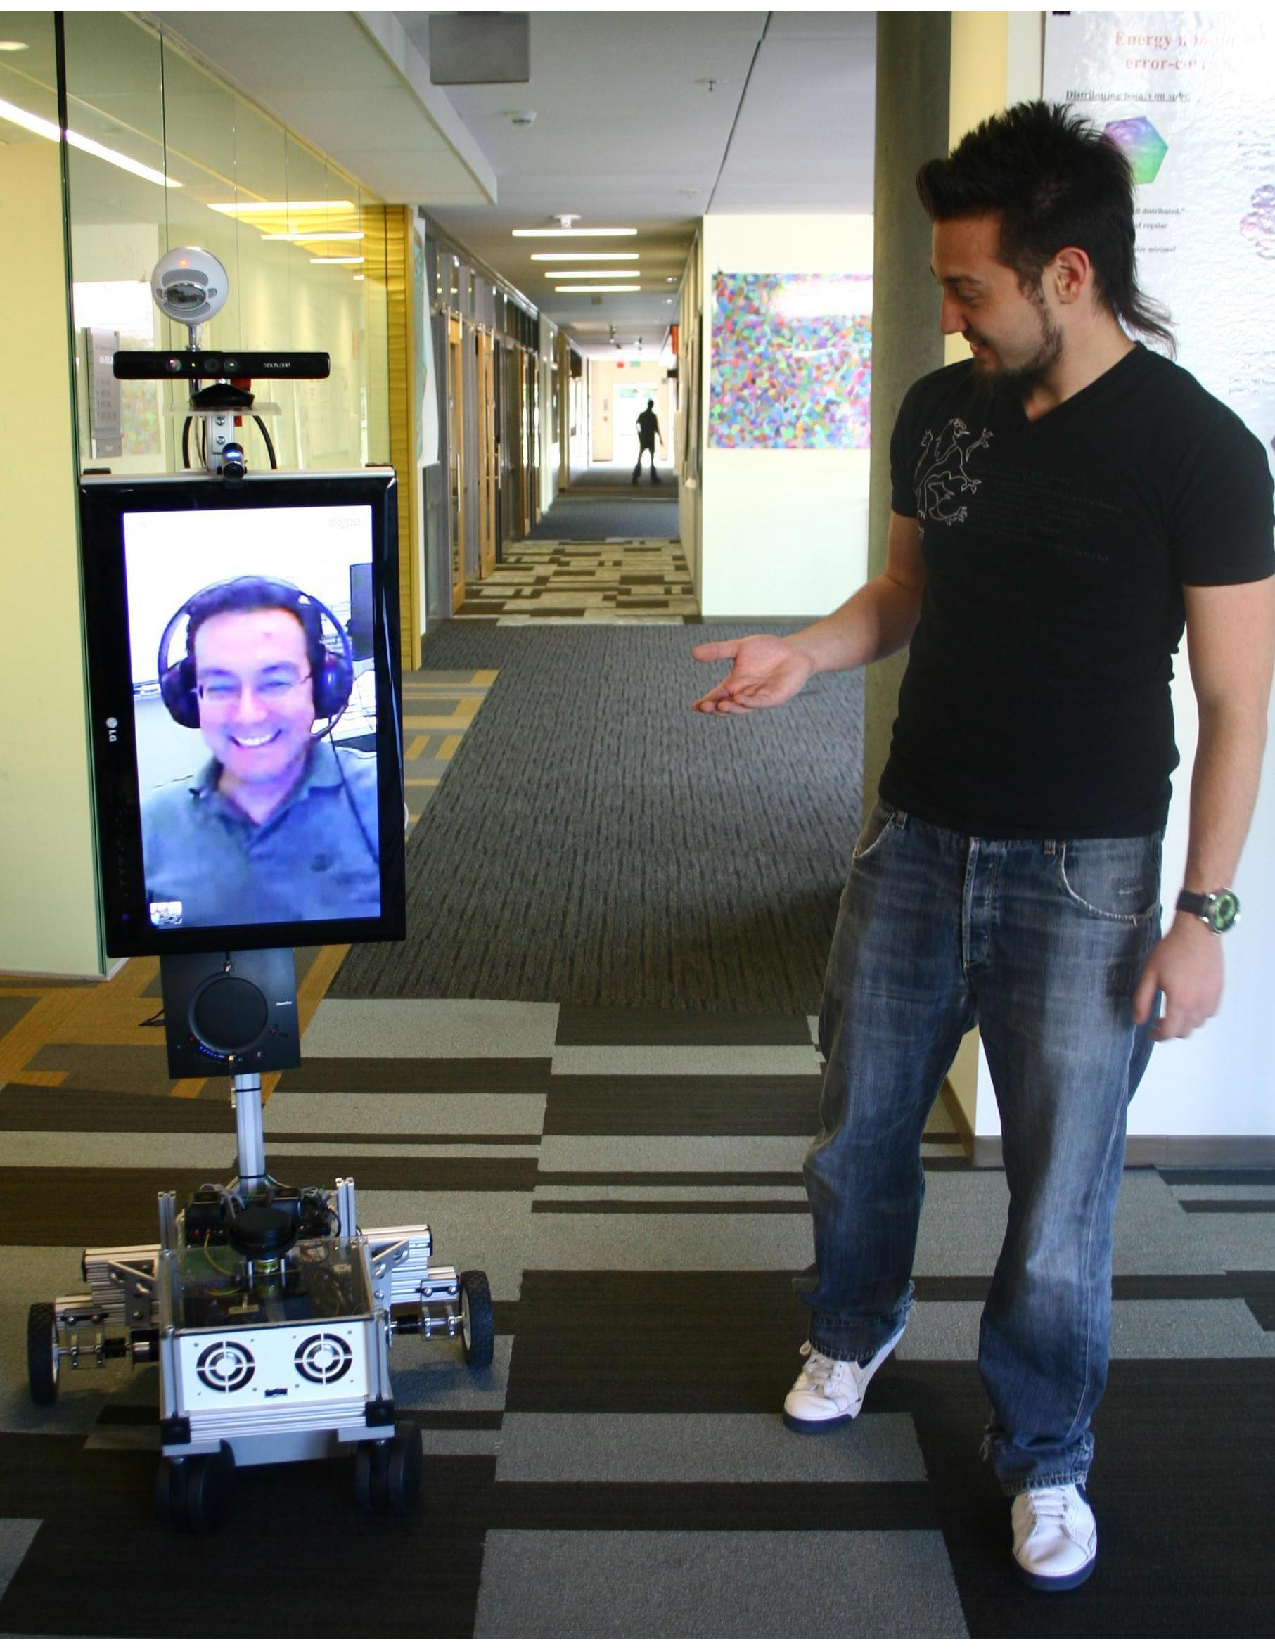
\includegraphics[width=0.4\textwidth]{pics/telepresence_robot}
\caption{The telepresence robot platform we used for our experiments.}
\label{fig:telepresence_robot}
\end{figure}

The system described in this paper is implemented on an experimental telepresence robot shown in Figure~\ref{fig:telepresence_robot}. The robot has a differential drive base and can be used for about 8 hours with full charge. For the experiments in this paper, the speed of the robot was limited to 0.55 m/s. A laser scanner with 360$^{\circ}$ field of view, which was taken from Neato XV-11 vacuum cleaning robot, was mounted horizontally at 0.3m height. The system runs on Windows 7 and Microsoft Robotics Developer Studio (MRDS) as its distributed computing environment. The remote user connects to the robot via wireless internet and communicates with others using Skype. On the remote end, . The robot is also equipped with an omni-directional microphone and a high-end speakerphone.

There are two operation modes for the robot: Teleoperation and Autonomous Person Following. A Xbox 360 Wireless Controller is used to remotely teleoperate the robot.  A wide-angle camera is placed on top of the monitor and tilted slightly downward to help the remote user to see the floor, robot base and people's faces at the same time. A Kinect Sensor is also placed above the monitor. Person following is initiated through the user interface shown in Figure \ref{fig:telepresence_ui}.

\begin{figure}[h!]
\centering
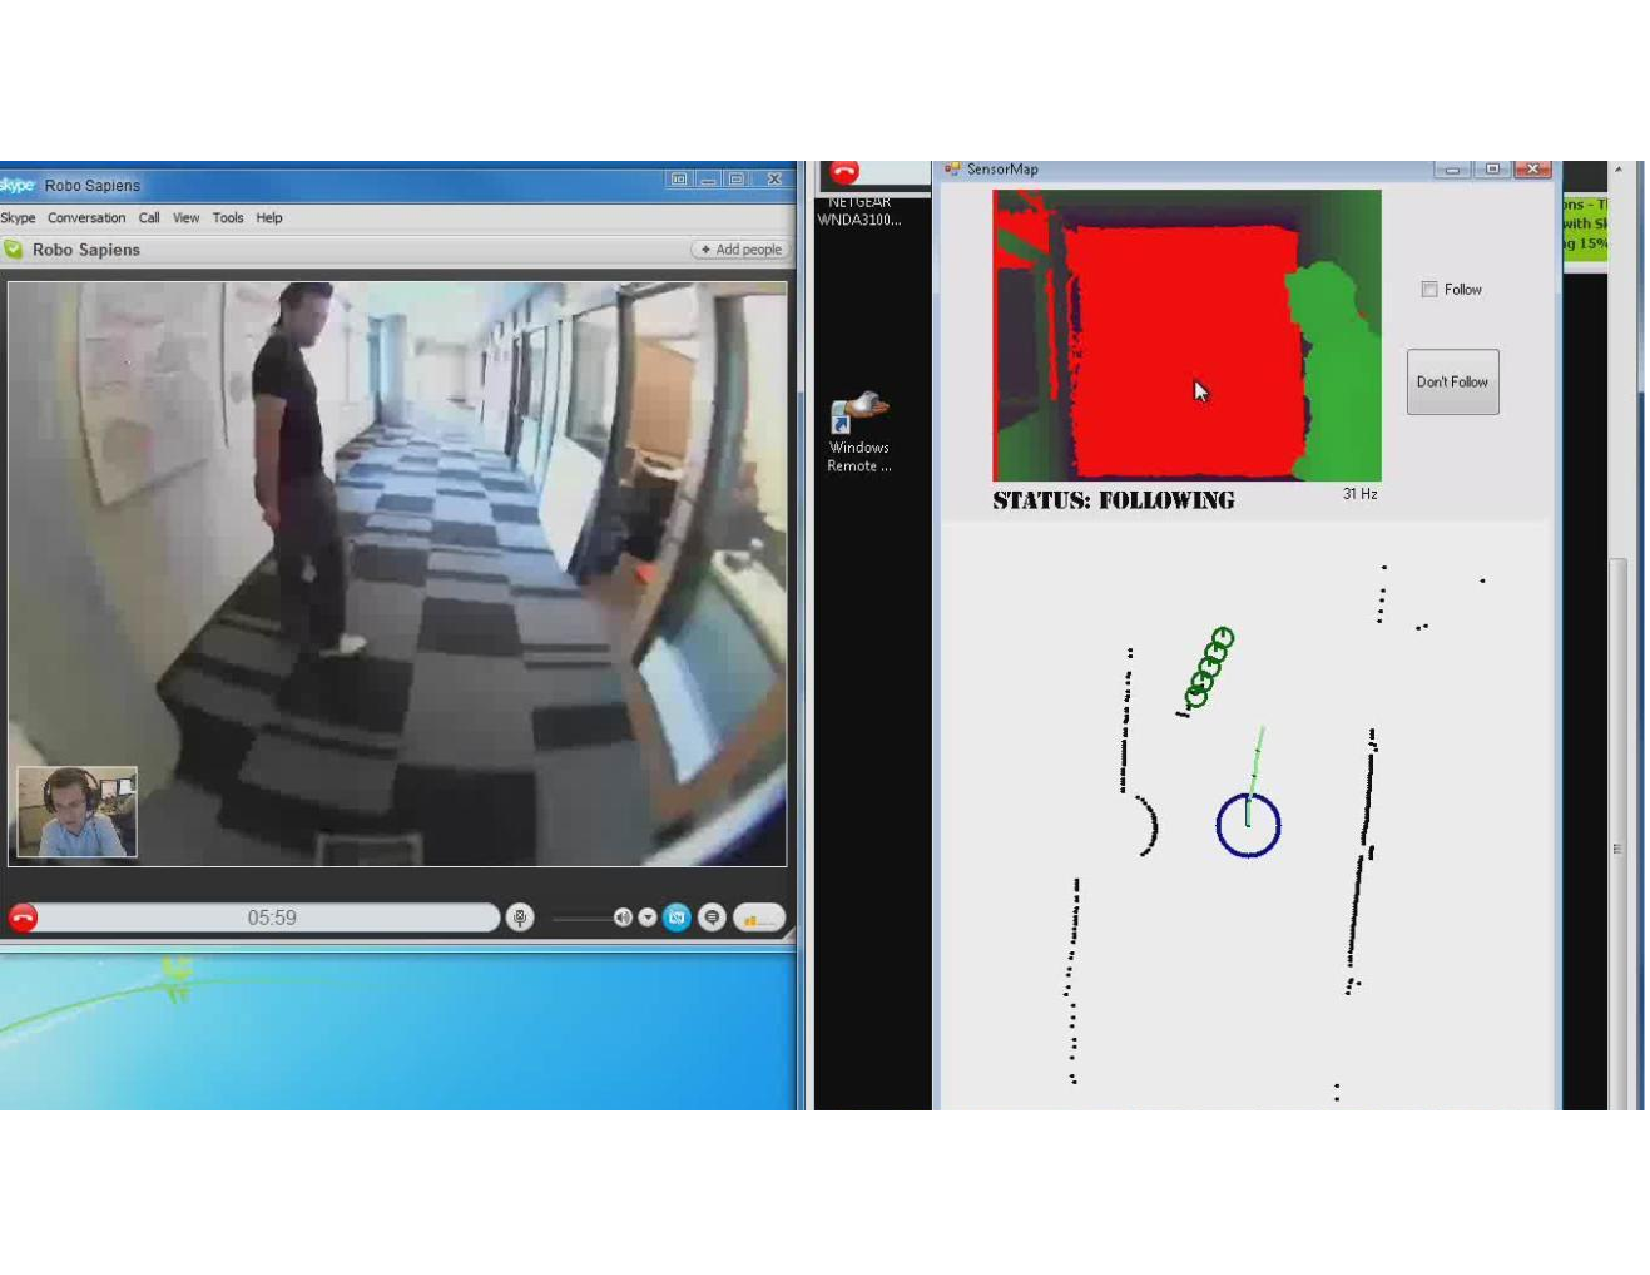
\includegraphics[width=1.0\textwidth]{pics/telepresence_ui_cropped}
\caption{User Interface of the robot for the remote user.}
\label{fig:telepresence_ui}
\end{figure}

A modified version of the local planner used in Section \ref{sec:navigation_local_planner} is used for person following. A utility function consisting multiple factors, including the respective position to the person, is optimized over multiple steps using Breadth-First Search. Details of the planning method can be found in \cite{cosgun2013autonomous}.

\subsection{User Study}

In this study, remote user is the subject and the followed person is the experimenter. To investigate the effectiveness of using autonomous person following for an interaction task, we ran a controlled experiment and varied manual vs. autonomous following within subjects.

\paragraph{Design:}
The experiments were conducted in working hours and bypassers were allowed to walk across the experiment area or talk. The subjects were given the task of following the experimenter through the course for a lap and listen to the passage he is reading. In the first run, the subject used the autonomous following or teleoperation method to follow a person and complete the lap. In the second run, the subject used the other method. At the end of each run, the subject was asked to complete a 4-question quiz about the passage. The passages and quiz questions were taken from Test of English as a Foreign Language (TOEFL) listening section examples. One passage was about ``behaviorism" and the other one was about ``manila hemps", and passages were chosen so that they are at a similar difficulty level. The time it takes to read a passage corresponded approximately to the same time a lap is completed. We also asked numbered 7 point Likert scale questions, administered after each run, about how \emph{Understandable} the experimenter was, \emph{Easiness of UI}, if the robot exhibited \emph {Natural Motions}, how \emph{Safe} the remote user felt, if the subject was able to \emph{Pay Attention} to the passage, how \emph{Fast} the robot was and how much \emph{Fun} the subject had. At the end of both runs, the user was asked which method he/she will prefer over the other for this type of a scenario. The exact questionnaire was show in Section/Appendix TODO.

\paragraph{Participants:}

10 volunteers participated in the study (6 male and 4 female between the ages of 25-48). Participants consisted of 4 researchers and 6 interns at Microsoft Research. 5 of the participants had little knowledge, 4 had average knowledge and 1 had above average knowledge on robotics. The participants weren't gamers: 4 participants never played console games, 4 played rarely, 1 sometimes played and 1 often played. 6 of the participants often used video conferencing software, while 2 sometimes and 2 rarely used. 9 of the participants were not native English speakers and all of them had taken the TOEFL before. Participants were recruited through personal relations and were given a small gift (valued at approximately US$ \$ $10) for their help.

\paragraph{Procedure:}

The participants were first greeted by the experimenter and instructed to complete a pre-task questionnaire regarding their background. The robot was shown to the participant and basic information about its capabilities was told. The experimenter explained the task while walking with the participant in the corridor and showing the course to be followed. Participants were told that they should stay close to the experimenter while he is walking and there will be a quiz regarding the passage afterwards. The participant was informed that there are 2 operation modes: manual and autonomous person following.

Before the experiment started, the participant went through training for about 15 minutes. First, the participant learned the basic controls for the Xbox controller when he/she was nearby the robot. Then the participant was taken to the remote station, which was in a room about 20 meters away from the corridor area. The participant was informed about the UI and was shown how the autonomous following can be activated. Then a test run was executed, where the remote user followed the experimenter via teleoperation and had a conversation.

After the training, the actual run was executed using either the manual or autonomous method. When the lap was completed, first the passage quiz, then the survey questions were answered by the subject. Then the second experiment using the other method was executed, and the second passage quiz and survey questions were given to the subject. As the last question, the subject was asked to state his/her method of preference. Lastly, the participants were debriefed about the study and engaged in a discussion. We switched the starting method for every other experiment in order not to bias the subjects' opinions about one particular method.

\paragraph{Measures:}
We had three measurement criteria to compare manual vs autonomous following: 1) Number of correct answers to passage quizzes: Assuming the standardized TOEFL exercises were of same difficulty, we ran a paired $t-test$ on two groups of autonomous and manual. 2) Survey questions: We ran a paired $t-test$ using 7-point Likert Scale on each of the seven questions. 3) Preferred Method: We looked at which method subjects chose over the other one.

\paragraph{Results:}

Out of 4 quiz questions, the correct answers for autonomous group ($\mu=2.9$, $\sigma=0.9$) were more than the manual group ($\mu=2.2$, $\sigma=1.2$) but the statistical difference was not statistically significant ($t(9)=1.48$, $p=0.17$ on $t-test$).

\begin{table}
	\centering
  \begin{tabular}{lSSSSSS}    
    \toprule
    \multirow{2}{*}{Question} &
      \multicolumn{2}{c}{Autonomous} &
      \multicolumn{2}{c}{Manual Drive} &
      \multicolumn{2}{c}{$t-test$} \\
      & {$\mu$} & {$\sigma$} & {$\mu$} & {$\sigma$} & {$p$} & {$t$} \\
      \midrule
    1. Understandable & 4.0&	1.5&	3.6&	1.7&	0.47 & 0.73 \\
    2. Easy UI & 6.5&	0.9&	5.0&2.2&0.06& 2.13 \\
    3. Natural Motion &  5.4 & 1.0& 3.5 & 1.9 & 0.03 & 2.52 \\
    4. Safe & 5.1 & 1.7 & 2.3 & 1.4 & 0.01 & 3.09 \\
    5. Pay Attention & 5.3 & 1.8 & 3.4 & 1.5 & 0.02 & 2.63 \\
    6. Fast & 3.9 & 0.3 & 4.3 & 0.8 & 0.10 & -1.8 \\
    7. Fun & 5.3 & 1.5 & 5.1 & 1.7 & 0.66 & 0.45 \\
    \bottomrule
  \end{tabular}
      \caption{Survey results of the user study for person following for telepresence robots. Table displays survey question average and standard deviations for the two conditions: Autonomous Person Following and Manual Person Following.}
    \label{table:telepresence_table}
\end{table}


Table \ref{table:telepresence_table} summarizes the survey results. For \emph{Understandable} and \emph{Fun}, the scores slightly favored autonomous method but the difference wasn't statistically significant. Manual method User Interface (gaming controller) was found to be easy to use ($\mu=5.0$, $\sigma=2.2$), but the UI for autonomous method (clicking) was found to be marginally easier ($\mu=6.5$, $\sigma=0.9$), ($t(9)=2.13$, $p=0.06$). The motions of the robot was found to be significantly more \emph{Natural} to have a conversation for autonomous ($\mu=5.4$, $\sigma=1.0$) than manual ($\mu=3.5$, $\sigma=1.9$), ($t(9)=2.52$, $p=0.03$). Participants thought they were able to \emph{Pay more Attention} to the passage the experimenter is reading when the robot was following the him autonomously ($\mu=5.3$, $\sigma=1.8$) compared to manual control ($\mu=3.4$, $\sigma=1.5$) and the statistical difference was significant ($t(9)=2.63$, $p=0.02$). Participants have found the autonomous method ($\mu=5.1$, $\sigma=1.7$) much safer than manual method ($\mu=2.3$, $\sigma=1.4$) and there was a significant difference between two groups ($t(9)=3.09$, $p=0.01$). The speed of the robot was found to be neither fast nor slow for both methods ($\mu=3.9$, $\sigma=0.3$) and ($\mu=4.3$, $\sigma=0.8$).

All 10 subjects chose autonomous person following over teleoperation for this task.




\subsection{Design Implications}

Our user study showed that a person following behavior is desirable for telepresence robots when there is interaction. The follow-up discussions also agreed with the survey results, as one subject (R10) stated: \emph{``It just gives me more focus and concentration.''} Below, we list our observations and implications for future research and design for telepresence robots:

\textbf{Motor Noise:} Even though the motors on the robot were relatively quiet, 8 out of 10 participants expressed that the motor noise made communication harder. This justifies the close scores we collected in the survey question asking if the subject was able to understand what the experimenter was saying. (R8) was disturbed by the noise: \emph{``When I was driving, it was always this constant sound. It was worse for the autonomous one. It was constantly adjusting and compensating for the movement."} On the other hand, (R5) found the motor noise useful: \emph{``I actually like it because it gives me the feedback whether I'm driving faster or slower. It also gives me a little bit feeling of life."} Thus, although excessive motor noise should be avoided, some noise might be useful.

\textbf{Wireless Connection:} Second most cited problem for video conferencing was the video quality and time lags. (R8) clearly expressed why it was hard to walk with the experimenter using the manual method: \emph{``The frame rate drops all of a sudden and you have no choice but to stop."} Another subject (R9) made use of the displayed sensor data when the video conferencing quality went bad: \emph{``Because of the lag, I just switched to the Kinect (depth image) and the overhead view (laser)."} This was possible because the wide angle camera image was coming from Skype whereas sensor displays were received from the Windows Remote Assistance. Clearly, a big challenge for telepresence systems is to deal with wireless connection problems.

\textbf{Natural Interaction:} Even though the participants thought the motions of the robot were natural to have a conversation ($\mu=5.4$, $\sigma=1.0$), some didn't feel it was a natural way to communicate. As seen in Figure \ref{fig:telepresence_robot}, the screen displaying the remote user's face is flat and it introduced problems when the robot was traveling on the side of the person. (R5), when asked about walking side by side: \emph{``..we don't have face-to-face. It is not really a conversation."} This raises design considerations on how the remote user's face is brought out. One of the subjects (R5) discovered that the microphone characteristics are different than human hearing: \emph{``I don't have a distance sense if the experimenter is further away or close. If you have the fading audio, then I'll immediately notice."} Whether a telepresence robot should exhibit the same characteristics of human perception or not is an open question and needs further investigation.

\textbf{Assisted Teleoperation:} Telepresence robots should possess a layer to assists the remote user to avoid obstacles and collisions. \emph{Safety} ratings for the manual method were very low ($\mu=2.3$, $\sigma=1.4$) and (R8) expressed the concern: \emph{``I was especially worried about running into the experimenter."} This suggests that scenarios involving interaction would demand more attention of the remote users. The teleoperation should also be intuitive and be similar to driving modalities that people are already used to. (R4) stated: \emph{``I was thinking about Manual mode compared to driving a car."} before suggesting \emph{``.. maybe something like a cruise control might be good."}

\textbf{Gaming Experience:} Since the robot was controlled by a gaming console controller, some participants likened the manual mode to gaming. (R9) said: \emph{``Manual is like playing video games."} and (R5) said: \emph{``I don't play video games so controlling those consoles is not natural to me."} Thus, it is possible that gamers are less likely to have trouble driving the robot. This observation is also made by Takayama \cite{takayama2011assisted}.

\textbf{Long Term Interaction:} None of the subjects participated in our study had used a telepresence robot before. (R6) justified the inability to use the manual method: \emph{``Maybe if I have some more practice for about several hours of driving the robot, I can use manual as well as autonomous.''} (R8) on having fun using teleoperation: \emph{``It was fun because it was the first time I did it but I can imagine that over time, I'll get bored of it."} The \emph{Fun} question in the survey received similar scores for autonomous and manual, possibly because using a telepresence robot was a new experience for the subjects. Studies regarding long term interaction for telepresence robots can yield interesting results, as in \cite{lee2011now}.

\textbf{Error recovery:} When the person was lost during following, the UI displayed a text that the person was lost so that the remote user can re-initiate the following by clicking on the person. None of the subjects complained about the robot losing the person. When asked explicitly about the robot losing the experimenter, (R10) answered: \emph{``That's not a big deal in comparison to me driving the robot."} Therefore, applications developed for telepresence robots can take advantage of the human being in the loop and does not have to be error-free for deployment.

\subsection{Discussion}

User studies showed that autonomous person following
is a desired capability for a telepresence robot and it was
favored over direct teleoperation for an accompanying task.
Autonomous following was found to be safer, easier to use
and helped the remote users to pay more attention to the
conversation instead of the robot control. From the experience
earned from user studies, there are still interesting
challenges to explore in terms of human-robot interaction for
telepresence robots.

%%%%%%%%%%%%%%%%%%%%%%
\chapter{Interactive Semantic Labeling}
\label{chapter:map_annotation}

World representation of robots should enable effortless communication between users and robots. Robots that co-exist with humans will need to accept commands from human users. As mentioned in Chapter \ref{chapter:introduction}, the robot keeps a metric map for autonomous navigation. Requiring users to understand the robot's internal representation of the world and to provide goals in terms of metric coordinates may not be a convenient way of interaction. For example, it is not easy for someone to quickly interpret the floor plan and provide a goal with explicit coordinates $(1.2,4.5,0.0)$. Maps should include spatial information to support tasks that requires more than simple obstacle avoidance. For example, if the task involves interaction with planar surfaces, landmarks, objects, or people; a robot's map should be able to represent these information. For these reasons, adding semantic information to robot maps is essential. There are several methods to support the annotation of entities in a robot map. For example, while the robot is building its representation of the environment, it can recognize objects or landmarks such as doors, tables, rooms and automatically add these features to its map. Even though such a system would be useful, it may wrongly label some objects. In that case, the correct label can be provided by a human with an interactive system. Custom labels would also allow unique annotations such as \textit{"John's Room"}.

We use a map representation that includes 2D waypoints, 3D polygons that defines the boundary of planar surfaces and objects along with user-appointed labels. We give more details about waypoint representations in Section \ref{sec:map_waypoints}, planar surfaces in Section \ref{sec:map_landmarks} and objects in Section \ref{sec:map_objects}. To add labeled landmarks and objects to the semantic map, we use an interactive system that uses a combination of a graphical user interface (GUI) and natural pointing gestures. Using the GUI, users can command the robot to follow them, add waypoints along the robot's path and add landmarks or objects to the map by pointing at them and entering a label. Our GUI is shown in Section \ref{sec:map_ui} and our approach to determine the pointing gesture targets is presented in Section \ref{sec:pointing_gestures}.

\section{Related Work}
\label{sec:map_relevant_work}

One of the key concepts in semantic mapping is establishing a \textit{common ground} \cite{clark1991grounding}. By referring to same structures and objects with the same reference, the communication about labeled entities is grounded.

One of the closely related works to our interactive labeling approach Human Augmented Mapping, introduced by Topp and Christensen in \cite{topp2006topological} and \cite{topp2010detecting}. This approach involves labeling two types of entities: regions and locations. Regions are meant to represent areas such as rooms and hallways, and serve as containers for locations. Locations are meant to represent specific important places in the environment, such as a position at which a robot should perform a task. This approach was applied to the Cosy Explorer system, described in \cite{zender2007integrated}, which includes a metric map, a topological map, as well as detected objects. While our goal is similar, we use a different map representation, method of labeling and interaction design. Kuipers \cite{kuipers2000spatial} introduced Spatial Semantic Hierarchy, which is a method of organizing semantic information for spatial regions. Another application using semantic maps is direction following, studied by Kollar \cite{kollar2010toward}. This work describes a system capable of following directions in natural language, i.e. ``go past the computers". People also routinely use semantic relationship of objects when they refer to objects. For example, the robot can handle a command such as ``get the mug on the table".

\section{Semantic Maps}
\label{sec:map_semantic_maps}

Semantic mapping aims to create maps that include various types of semantic information to allow the robot to have a richer representation of the environment. In this section, we briefly present the semantic information we use to enrich the occupancy grid maps: waypoints, planar landmarks and objects. Although we describe three types of entities for storing semantic information, it is possible to include more features.

\subsection{Navigation Waypoints}
\label{sec:map_waypoints}

We define navigation waypoint as a navigable pose represented in the map frame. A pose $(x,y,\theta)$ represents the position and orientation of with respect to a coordinate frame. We will refer a navigation waypoint simply as a waypoint for the remainder of this text. Using the GUI, a user can save the robot's current pose along with a label, assuming that the robot is properly localized in the map. This method is the most straightforward way to save a pose and use it later for a task. When the robot is asked to navigate to a labeled waypoint, the goal of the robot is simply the saved pose.

Even though the waypoint method is easy to use and practical, it has shortcomings. It fails to capture the shape and extent of the structure designated by the label, which might be important for some tasks, such as object search. Moreover, point based references may be ambiguous to represent a region or volume in a map, such as a hallway or a room. For example, if the user wants to save hallway as a landmark, it is useful to have a representation of the location and the extent of the hallway. Another example is that the user can label a coffee table, which is a movable object. Instead of saving a fixed coordinate location for the landmark, robot can save the planar surface and can potentially have a model to handle moving landmarks. This gives the robot robustness in its operations and a method to potentially use the planar surfaces as features in localization \cite{trevor2012planar}.

\subsection{Planar Surfaces}
\label{sec:map_landmarks}

In this type of semantic information, we keep track of a set of observed planar surfaces as part of the map representation. We use a front-facing RGB-D camera to acquire suitable data. Planes are extracted from the point cloud by an iterative RANdom SAmple Consensus (RANSAC) method, which allows us to find all planes meeting constraints for size and number of inliers. A clustering step is performed on extracted planes to separate multiple coplanar surfaces, such as two tables with the same height, but at different locations. We make use of the Point Cloud Library (PCL) \cite{rusu20113d} for much of our point cloud processing. Planes are represented in the hessian normal form. Since the observed planes do not have infinite extent, we bound the observed area with a polygon - in this case, the convex hull of all the observed points on the plane. The convex hull is accompanied with a user-provided label. 

In order to label a planar landmark, the user goes through the following sequence:

\begin{enumerate}
\item User activates basic person following behavior (Section \ref{sec:following_basic_person_following}) and comes near a planar surface of interest.
\item Robot adjusts its pose so it can perceive both the surface and the user.
\item User enters the label using the GUI and activates pointing gesture recognition
\item User performs a pointing gesture towards the landmarks of interest
\end{enumerate}

The act of labeling a planar surface with a label "Table" from the view of the RGB-D camera planted on the robot is shown in Figure \ref{fig:pointing_table_desk}. After the labeling process, the planar landmark is added to the map representation.

\begin{figure}[ht!]
\centering
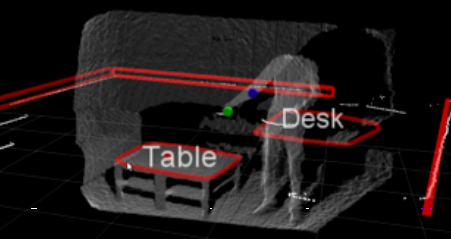
\includegraphics[width=0.55\textwidth]{pics/pointing_table_desk}
\caption{A user is pointing at a table to add it to the semantic map}
\label{fig:pointing_table_desk}
\end{figure}

\subsection{Objects}
\label{sec:map_objects}

Our approach allows interactively building object models for selected objects, and then annotate these models with a label. This enables the robot to quickly build a small object database of the specific objects it needs to interact with. The interactive system works as described in the previous section. Different from labeling planar landmarks, however, we keep a bag of features for each object in the database. Once a user has performed a pointing gesture to label objects, the robot moves to a favorable position and activates its its pan-tilt unit to aim the sensors at this location. Object segmentation is performed using point cloud data from an RGB-D sensor. First, the large planar surface corresponding to the table is detected. This is removed from the point cloud, and point clusters above this are detected. The robot calculates the likelihood of each object being the target, as will be explained in Section \ref{sec:pointing_gestures} and confirms with user if ambiguity is detected. After the target is confirmed, the cluster points are projected into the camera image, and are used to generate a region of interest. SURF features are found in the region of interest, and are stored as an object model along with the provided label.

\section{Graphical User Interface}
\label{sec:map_ui}

We developed an on-board tablet interface to enable interaction between the user and the robot. Similar functionality could be achieved with a speech recognition system, however we think a touch interface is a more robust type of communication. The interface has been implemented on a Nexus 7 Tablet running on Android Operating System. The tablet is equipped with WiFi and talks with the robot using a TCP-based server-client communication model. The client must have the the IP address of the server machine to establish the connection. The messages are sent back-and forth as via XML files. The XML files are serialized and de-serialized using \textit{libXML++} for \textit{C++} (server) and \textit{XMLPullParser} (client) for Android OS. With the tablet interface, a user can do the following:

\begin{itemize}
\item Add/Delete a Labeled or Generic waypoint
\item Label a Planar Surface or Object
\item Initiate Person Following
\item Initiate Person Guidance to a Labeled Planar Surface/Object/Waypoint
\item Stop Robot
\item Change IP Address and Port of the TCP connection
\end{itemize}

A screenshot of our tablet user interface is shown in Figure \ref{fig:ui}.

\begin{figure}[ht!]
\centering
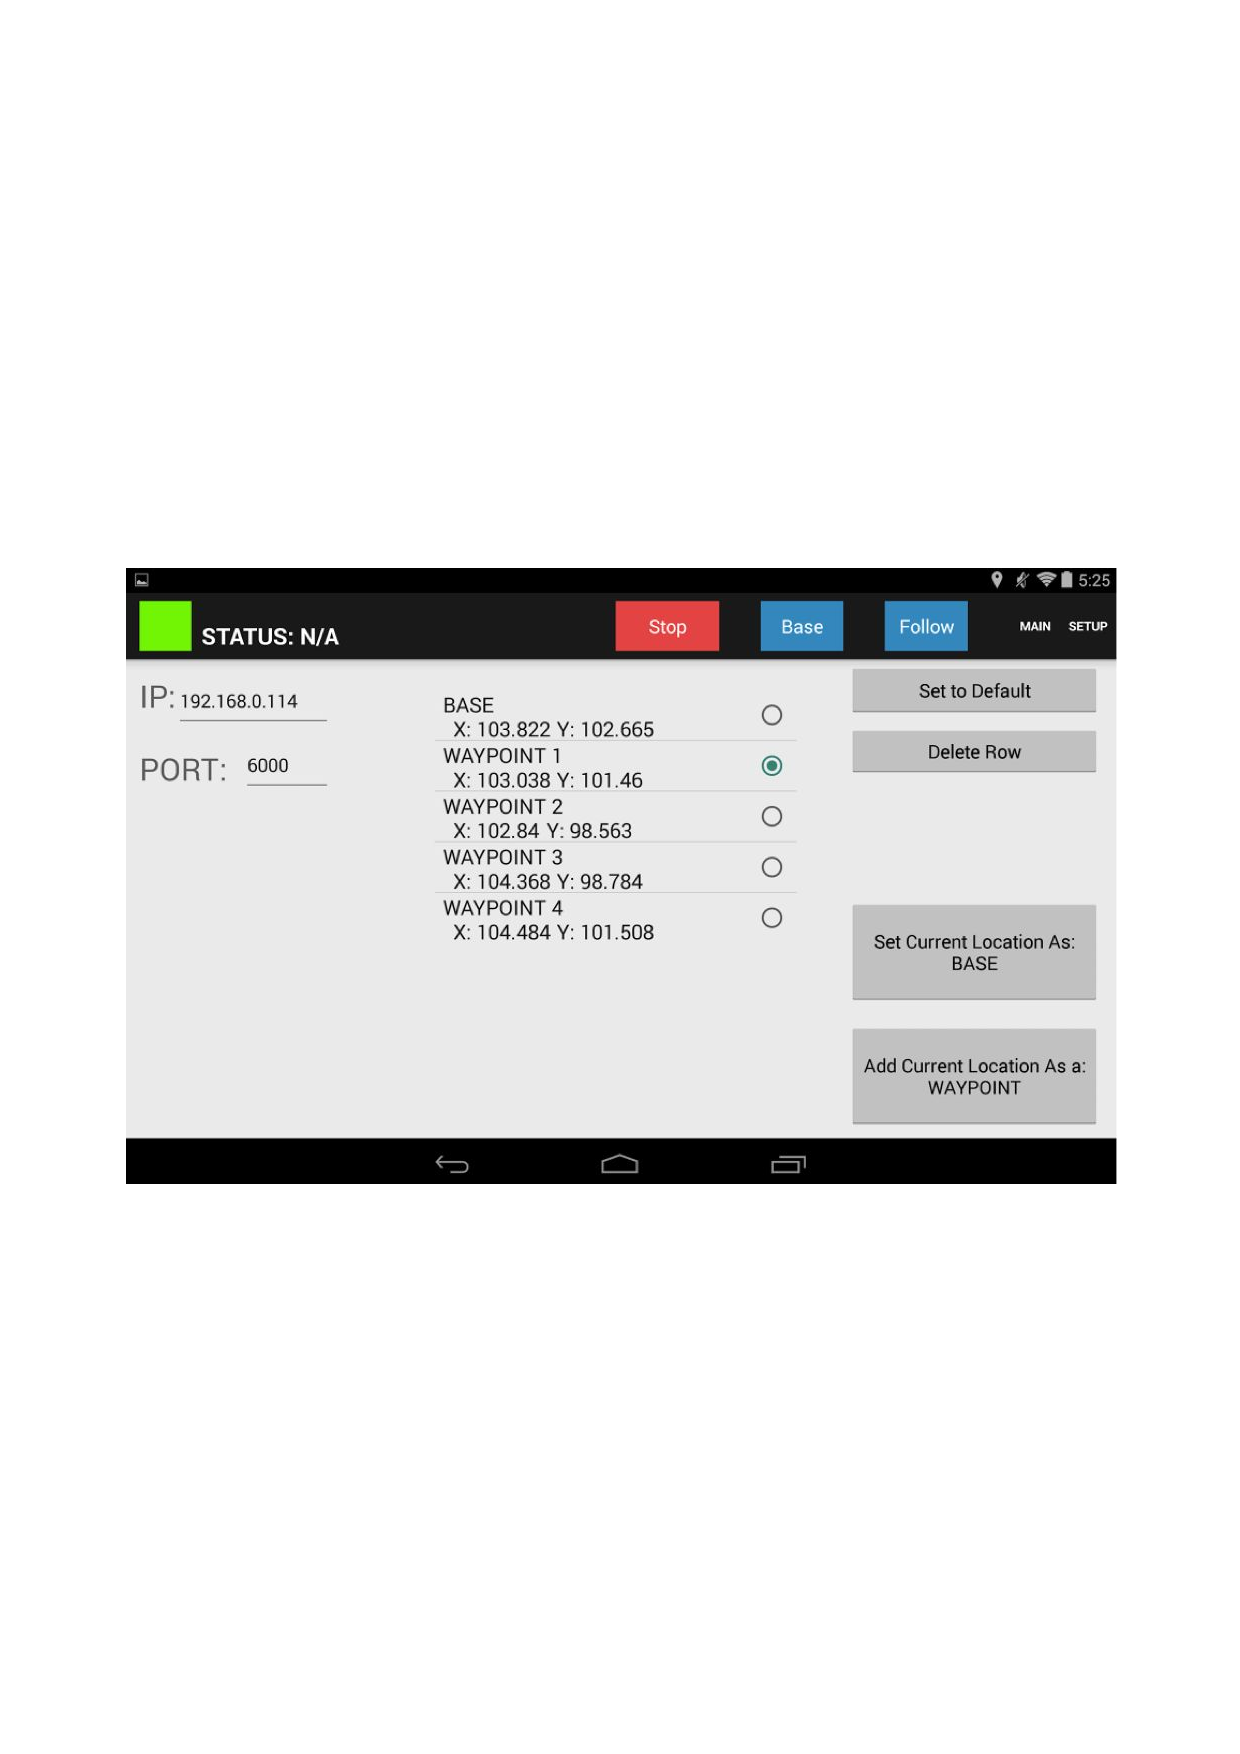
\includegraphics[width=0.75\textwidth]{pics/ui}
\caption{A snapshot from the GUI that runs on robot's touch screen}
\label{fig:ui}
\end{figure}

\section{Pointing Gestures for Human-Robot Interaction}
\label{sec:pointing_gestures}

A natural way to refer to objects and landmarks is to point at them. In this work, we analyze the performance of our pointing gesture recognition, and present an uncertainty model that enables us to reason about ambiguity in pointing gestures, when gesture targets are too close to one another. We model the uncertainty of pointing gestures in a spherical coordinate system, use this model to determine the correct pointing target, and detect when there is ambiguity. Two pointing methods are evaluated using two skeleton tracking algorithms: elbow-hand and head-hand rays, using both OpenNI NITE and Microsoft Kinect SDK~\cite{shotton2011real}.  A data collection with 6 users and 7 pointing targets was performed, and the data was used to model users pointing behavior.  The resulting model was evaluated for its ability to distinguish between potential pointing targets, and to detect when the target is ambiguous.  An example scenario is shown in Figure \ref{fig:cover_pointing_gestures}.

\begin{figure}[ht!]
\centering
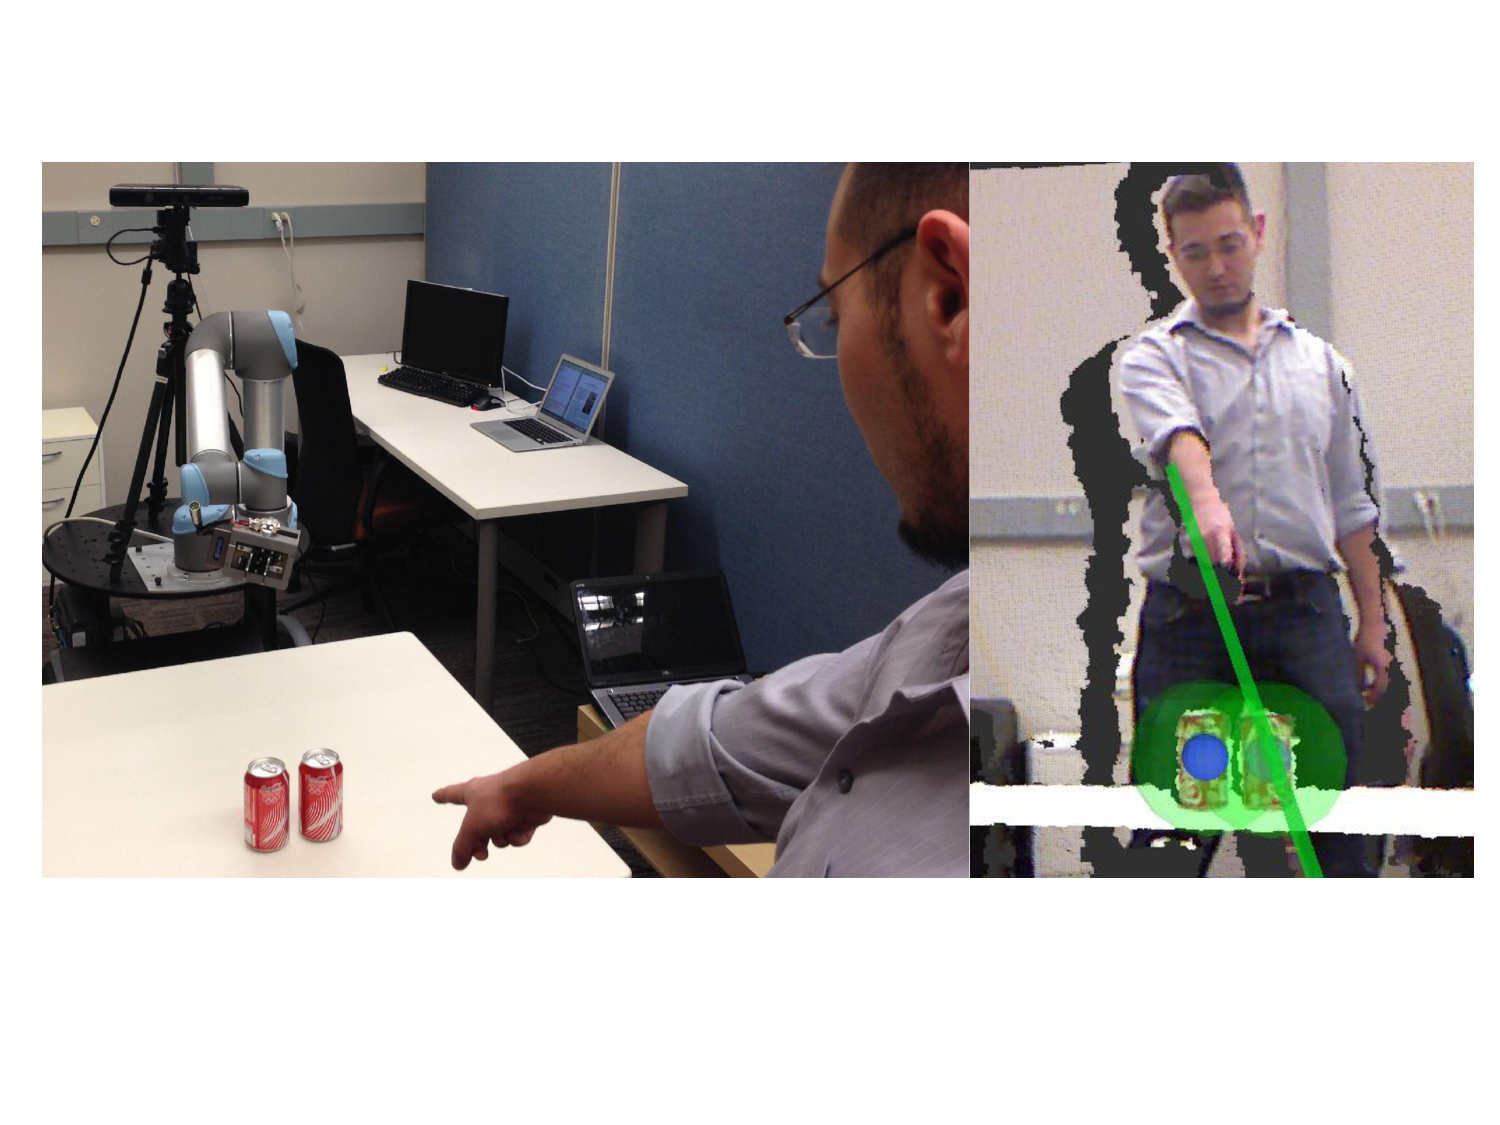
\includegraphics[width=0.8\textwidth]{pics/cover_pointing_gestures}
\caption{(Left) Our approach allows a robot to detect when there is ambiguity on the pointing gesture targets. (Right) The point cloud view from robot's perspective is shown. In this demonstration, both objects are identified as potential intended targets, therefore the robot decides that there is ambiguity.}
\label{fig:cover_pointing_gestures}
\end{figure}

\subsection{Related Works}
\label{sec:pointing_related_works}

Pointing gestures are widely used in Human-Robot Interaction applications. Examples include interpretation of spoken requests~\cite{zukerman2010interpreting}, pick and place tasks~\cite{blodow2011inferring}, joint attention~\cite{droeschel2011towards}, referring to places~\cite{hato2010pointing} or objects~\cite{schmidt2008interacting}, instructing~\cite{martin2010estimation} and providing navigation goals to a robot~\cite{raza2013human}. 

Early works on recognizing pointing gestures using stereo vision utilized background subtraction~\cite{cipolla1996human,jojic2000detection,kahn1995understanding}. Other popular methods include body silhouettes~\cite{kehl2004real}, hand poses~\cite{hu2010hand}, motion analysis~\cite{matikainen2011prop} and Hidden Markov Models~\cite{wilson1999parametric, bennewitz2008robust, li2005hierarchical, nickel2003pointing, droeschel2011learning, aly2012integrated}. Matuszek~\cite{matuszek2014learning} presented a method for detecting deictic gestures given a set of detected tabletop objects, by first segmenting the users hands and computing the most distal point form the user, then applying a Hierarchical Matching Pursuit on these points over time. 

After deciding if a pointing gesture occurred or not, an algorithm must estimate the direction of pointing. This is typically done by extending a ray from one body part to another. Several body part pairs are used in the literature, such as eye-fingertip~\cite{kehl2004real} and shoulder-hand~\cite{hosoya2004arm}; with the two of most commonly used methods being elbow-hand~\cite{raza2013human, brooks2006working, blodow2011inferring} and head-hand~\cite{bennewitz2008robust, schmidt2008interacting} rays. Some studies found that head-hand approach is a more accurate way for estimating pointing direction than elbow-hand~\cite{quintero2013sepo, droeschel2011towards}. Recent works made use of skeleton tracking data  in depth images~\cite{quintero2013sepo, blodow2011inferring, raza2013human}. Other approaches, such as measuring head orientation with a magnetic sensor~\cite{nickel2003pointing} and pointing with a laser pointer~\cite{cheng2009hand, kemp2008point} is reported to have a better estimation accuracy than the body parts method, but require additional hardware. We prefer not to use additional devices in order for the interaction to be as effortless as possible.

Given a pointing direction, several methods have been proposed to determine which target or object is referred by the gesture, including euclidean distance on a planar surface~\cite{cheng2009hand}, ray-to-cluster intersection in point clouds~\cite{blodow2011inferring, quintero2013sepo} and searching a region in interest around the intersection point~\cite{schmidt2008interacting}. Droeschel~\cite{droeschel2011learning} trains a function using head-hand, elbow-hand and shoulder-hand features with Gaussian Process Regression and reports a significant improvement on pointing accuracy. Some efforts fuse speech with pointing gestures for multi-modal Human-Robot Interaction~\cite{aly2012integrated,kowadlo2010influence}. Aly~\cite{aly2012integrated} focuses on relation between non-verbal arm gestures and para-verbal communication based on a HMM approach.

To our knowledge, only Zukerman~\cite{zukerman2011speaking} and Kowadlo~\cite{kowadlo2010influence} considered a probabilistic model for determining the referred object for a pointing gesture. In their approach, the probability that the user intended an object is calculated using the 2D distance to the object and the occlusion factor. Objects that reside in a Gaussian cone emanating from the user's hand are considered as candidates in the model. The approach is implemented in~\cite{zukerman2011speaking}, where it is reported that due to high variance of the gesture recognition system, the Gaussian cone typically encompassed about five objects in cluttered settings. Our work addresses the confusion in such settings. In contrast to their work, we measure Mahalanobis distances to potential target objects using a prior error analysis.

\subsection{Pointing Gesture Recognition}
\label{sec:pointing_pointing_gesture_recognition}

Our approach to pointing gesture recognition is to use a third party skeleton tracking package as implemented by OpenNI NITE 1.5 (OpenNI) or Microsoft Kinect SDK 1.5 (MS-SDK). Skeleton tracking software produces 3D positions for several important points and joint positions on the user's body, including hands, elbows, shoulders and head. We use the user's hands, elbows, and head for the recognition of pointing gestures. We are primarily interested in deictic gestures generated by pointing with one's arm. We consider two rays for determining the pointing direction: elbow-hand and head-hand. Both of these methods were evaluated with the two skeleton tracking implementations. For each depth frame, this yields two rays for each of the OpenNI and MS-SDK trackers:

\begin{itemize}
\item{$\vec{v}_{eh} := \vec{p_{elbow}p_{hand}}$}
\item{$\vec{v}_{hh} := \vec{p_{head}p_{hand}}$}
\end{itemize}


When a pointing gesture recognition request is received from a higher level process, the gesture is searched in a time window of \emph{T} seconds. Two conditions must be met to trigger a pointing gesture:

\begin{itemize}
  \item $\vec{v}_{eh}$ makes an angle more than $\phi_{g}$ with the vertical axis
  \item $p_{elbow}$ and $p_{hand}$ stays near-constant for duration $\Delta t_{g}$
\end{itemize}

The first condition requires the arm of the person to be extended away from his/her body, while the second ensures that the gesture is consistent for some time period. The parameters are empirically determined as: $\emph{T}=30s$, $\phi_{g}=45^{\circ}$ and $\Delta t_{g}=0.5s$.

\subsection{Representing Pointing Directions}
\label{sec:pointing_representing_pointing_directions}

We represent a pointing ray in two angles: a ``horizontal'' / ``azimuth'' sense we denote as $\theta$ and a ``vertical'' / ``altitude'' sense we denote as $\psi$. We first attach a coordinate frame to the hand point, with its z-axis oriented in either Elbow-hand $\vec{v}_{eh}$ or Head-Hand $\vec{v}_{hh}$ directions, depending on which method is used. The hand point was chosen as the origin for this coordinate system because both of head-hand and elbow-hand pointing methods include the user's hand. The transformation between the sensor frame and the hand frame $^{sensor}T_{hand}$ is calculated by using an angle-axis rotation. An illustration of the hand coordinate frame for Elbow-Hand method and corresponding angles are shown graphically in Figure \ref{fig:pointing_angle_errors}.

\begin{figure}[ht!]
\centering
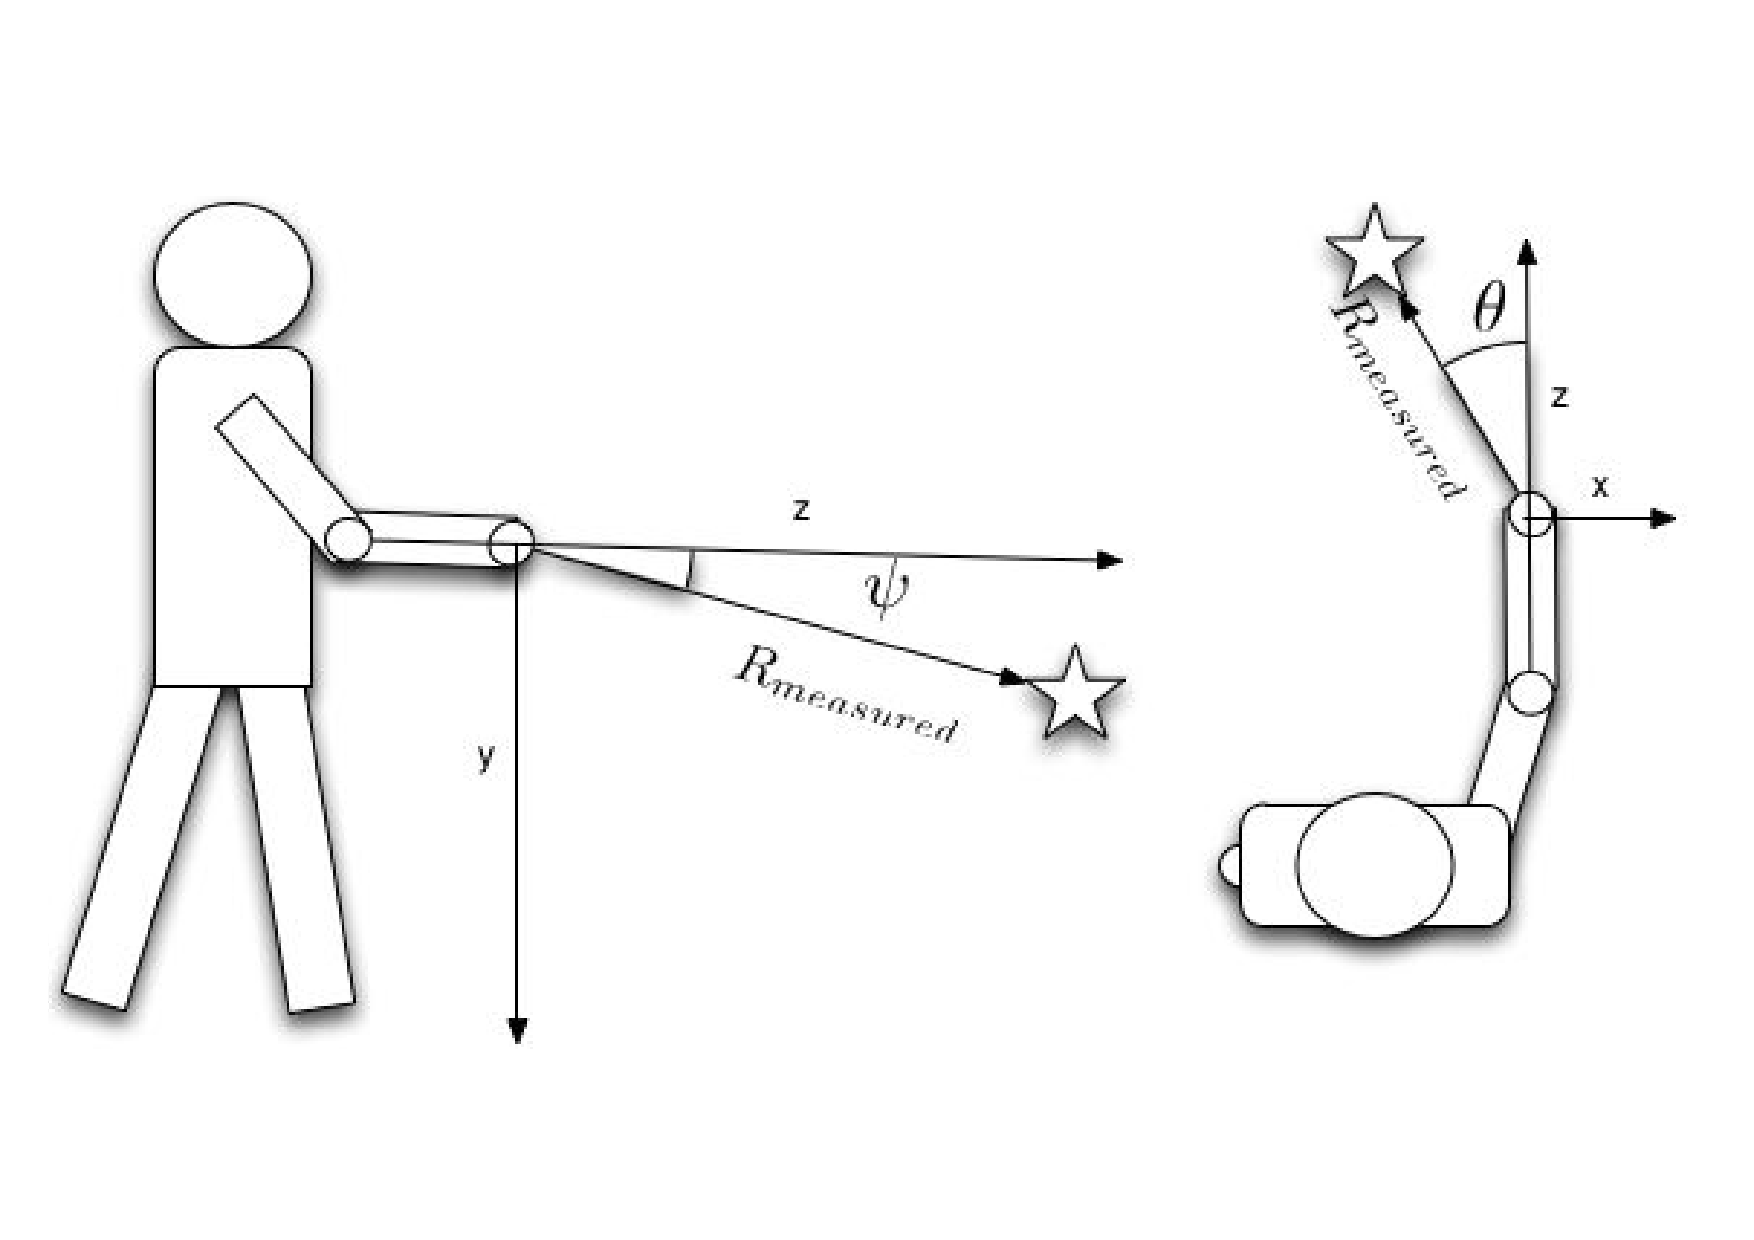
\includegraphics[width=0.8\textwidth]{pics/person_angles_combined_2}
\caption{Vertical $(\psi)$ and horizontal $(\theta)$ angles in spherical coordinates are illustrated. A potential intended target is shown as a star. The z-axis of the hand coordinate frame is defined by either the Elbow-Hand (this example) or Head-Hand ray.}
\label{fig:pointing_angle_errors}
\end{figure}

Given this coordinate frame and a potential target point P, we first transform it to the hand frame by:
$$^{hand}p_{target} = T_{hand} * p_{target}$$

We calculate the horizontal and vertical angles for a target point as $^{hand}p_{target} = (x_{targ}, y_{targ}, z_{targ})$ follows:
$$[\theta_{target}\;\psi_{target}]=[atan2(x_{targ}, z_{targ})\;atan2(y_{targ}, z_{targ})]$$

Where $atan2(y,x)$ is a function returns the value of the angle $\arctan(\frac{y}{x})$ with the correct sign. This representation allows us to calculate the angular errors in our error analysis experiments in Section \ref{sec:pointing_error_analysis}. The angles for each object is then used to find the intended target, as explained in the following section.


\subsection{Determining Intended Target}
\label{sec:pointing_determining_intended_target}

We propose a probabilistic approach to determine the referred target by using statistical data from previous pointing gesture observations. We observed that head-hand and elbow-hand methods, implemented using two skeleton trackers, returned different angular errors in spherical coordinates. Our approach relies on learning statistics of each of these approaches, and compensating for the error when the target object is searched for. First, given a set of prior pointing observations, we calculate the mean and variance of the vertical and horizontal angle errors for each pointing method. This analysis will be presented in Section \ref{sec:pointing_error_analysis}. Given an input gesture, we apply correction to the pointing direction and find the Mahalanobis distance to each object in the scene.

When a pointing gesture is recognized, and the angle pair $$[\theta_{target}\;\psi_{target}]$$ is found as described in the previous section, we first apply a correction by subtracting the mean terms from measured angles:
$$[\theta_{cor}\;\;\psi_{cor}]=[\theta_{target}-\mu_{\theta}\;\;\;\psi_{target}-\mu_{\psi}]$$
 
We also compute a covariance matrix for angle errors in this spherical coordinate system: 
$$S_{type} = \begin{bmatrix}
\sigma_{\theta}&0\\ 0&\sigma_{\psi}
\end{bmatrix} $$

We get the values for $\mu_{\theta}, \mu_{\psi}, \sigma_{\theta} ,\sigma_{\psi}$ from Tables \ref{table:pointing_horizontal} and \ref{table:pointing_vertical} for the corresponding gesture type and target. We then compute the mahalanobis distance to the target by:
$$D_{mah}(target,method)=\sqrt{ [\theta_{cor}\;\psi_{cor}]^T S_{method}^{-1} [\theta_{cor}\;\psi_{cor}]}$$
 
We use $D_{mah}$ to estimate which target or object is intended. We consider two use cases: the objects are represented as a 3D point or a point cloud. For point targets, we first filter out targets that have a Mahalanobis distance larger than a threshold $D_{mah} > D_{thresh}$. If none of the targets has a $D_{mah}$ lower than the threshold, then we say the user did not point to any targets. If there are multiple targets that has $D_{mah} <= D_{thresh}$ , then we determine ambiguity by employing a ratio test. The ratio of the least $D_{mah}$ and the second-least $D_{mah}$ among all targets is compared with a threshold to determine if there is ambiguity. If the ratio is higher than a threshold, then the robot can ask the person to resolve the ambiguity.

If the target objects are represented as a point cloud, we then compute the horizontal and vertical angles for every point in the point cloud and find the minimum mahalanobis distance among all. The distance to an object is then represented by this minimum value. Usage of the point cloud instead of the centroid for determining the intended object has several advantages. First, it yields better estimations due to the coverage of the full point cloud. Second, it takes into account the size of the object. For example, if a person is pointing to a chair or door, it is very unlikely that he/she will target the exact center. If the point cloud is used, then we can easily tell that the object is targeted.

 
\subsection{Data Collection}
\label{sec:pointing_data_collection}

To evaluate the accuracy of pointing gestures, we created a test environment with 7 targets placed on planar surfaces in view of a Kinect sensor (Figure \ref{fig:ground_truth_targets}). Depth data was collected from six users, who pointed at each of the seven targets with their right arm while standing at 2 meters away from the sensor. Targets 1 through 4 were on tables positioned around the user, while targets 5 through 7 were located on a wall to the user's right. Our use case is on a mobile robot platform capable of positioning itself relative to the user.  For this reason, we can assume that the user is always centered in the image, as the robot can easily rotate to face the user and can position itself at a desired distance from the user.

\begin{figure}[ht!]
\centering
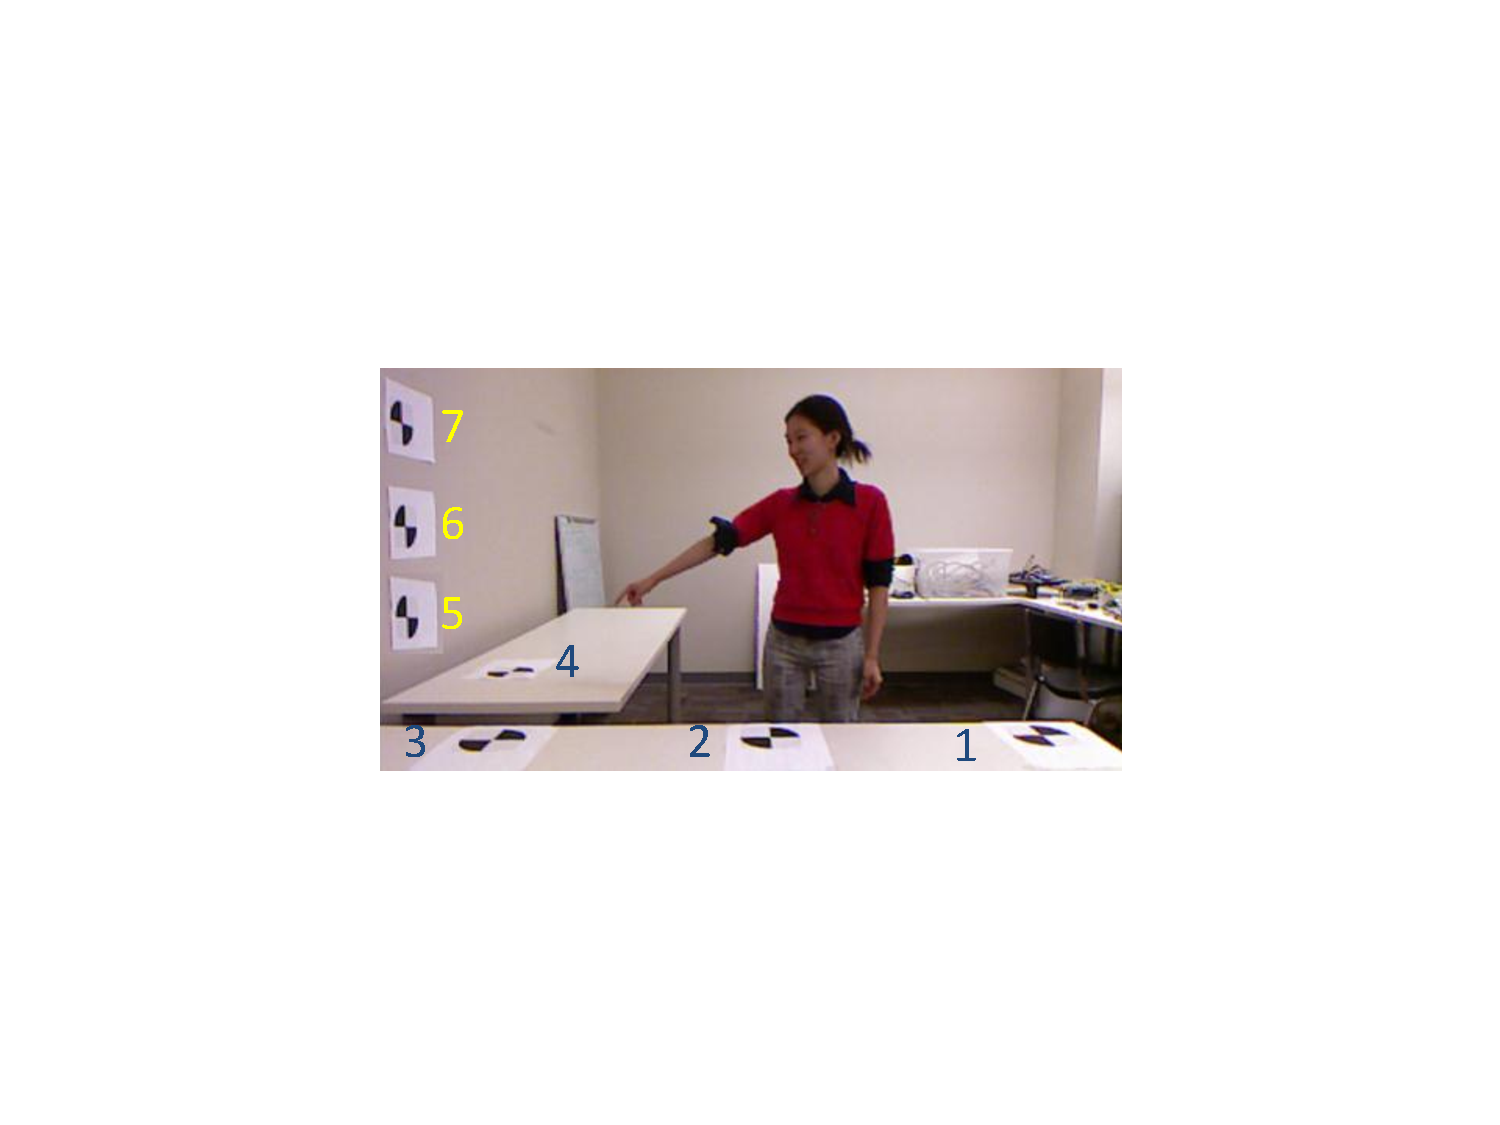
\includegraphics[width=0.65\textwidth]{pics/data_collection_crop}
\caption{Our study involved 6 users that pointed to 7 targets while being recorded using 30 frames per target.}
\label{fig:ground_truth_targets}
\end{figure}

\subsection{Ground Truth Target Positions}
\label{sec:ground_truth_points}

We make use of a plane extraction technique from a point cloud to have an accurate ground truth measurement. First, the two table and wall planes are extracted from the point cloud data using the planar segmentation technique described in \cite{trevor2013segmentation}. We then find the pixel coordinates of corners on targets in RGB images, using Harris corner detection \cite{harris1988combined}, which produces calculated corners in image coordinates with sub-pixel accuracy. The pixel coordinate corresponding to each target defines a ray in 3D space relative to the Kinect's RGB camera frame. These rays are then intersected with the planes detected from the depth data, yielding the 3D coordinates of the targets.



\subsection{Skeleton Data Capture}
\label{sec:pointing_skeleton_data_capture}

\begin{figure}[h]
\centering
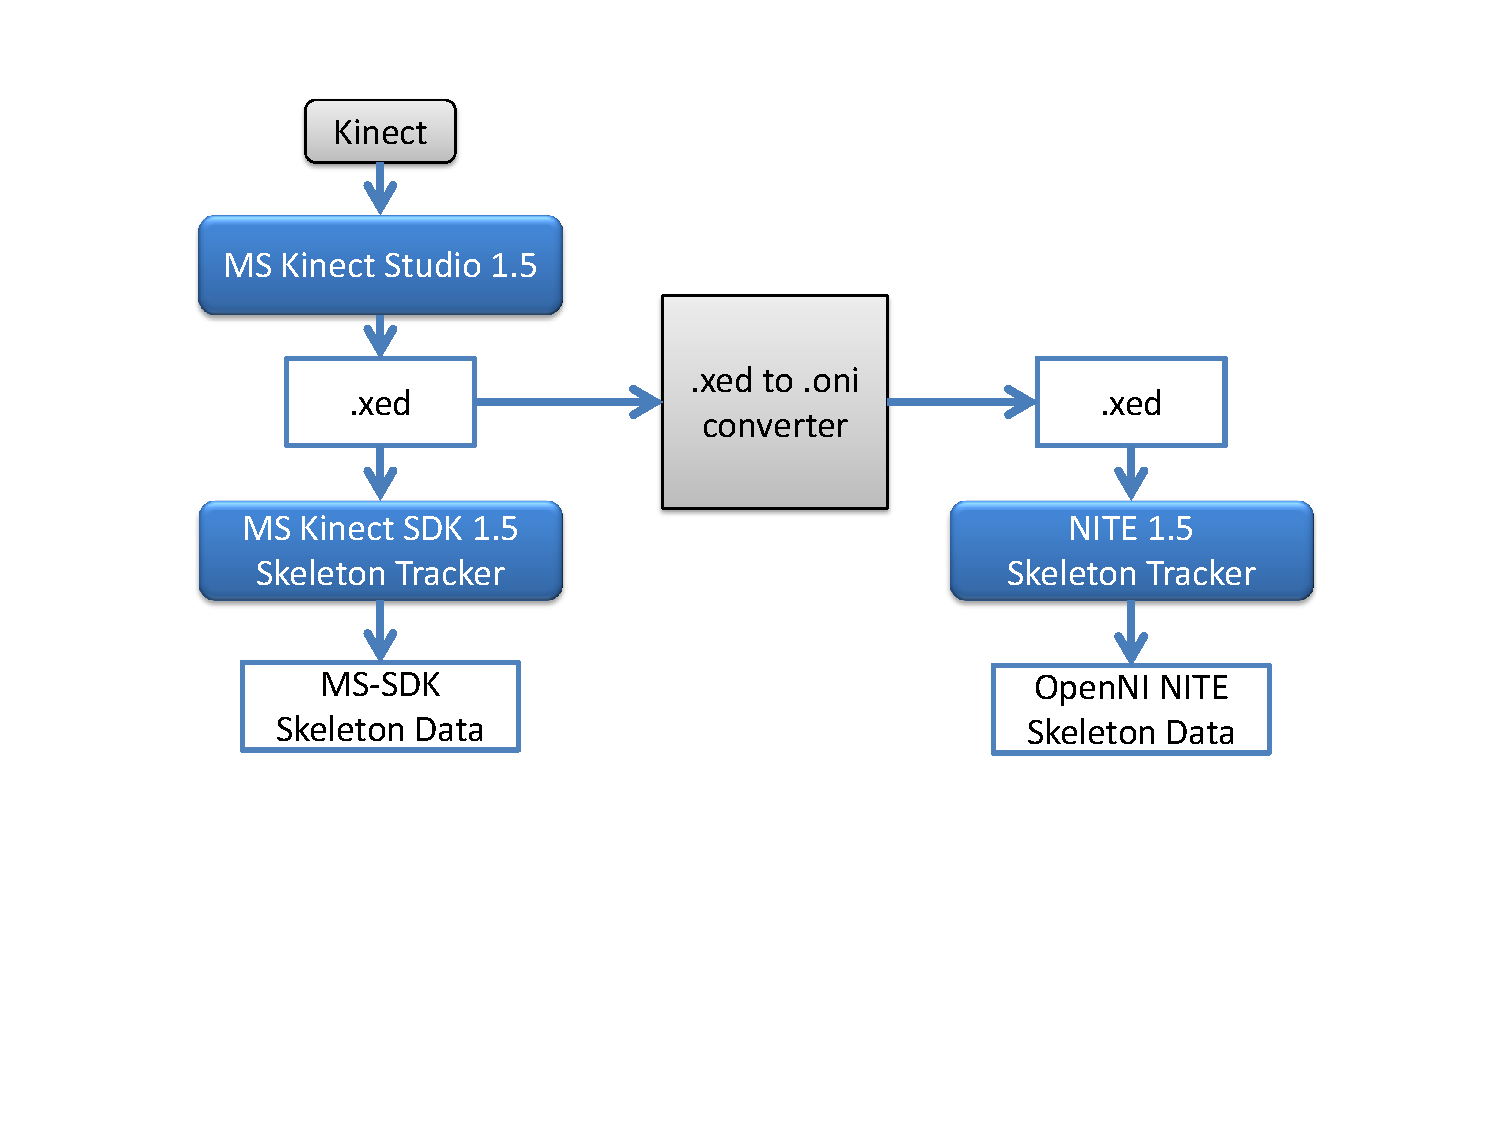
\includegraphics[width=0.75\textwidth]{pics/xedoni_2_cropped}
\caption{Data capturing pipeline for error analysis.}
\label{fig:xedoni}
\end{figure}

In order to be able to do a fair comparison between MS-SDK and OpenNI skeleton trackers, we used the same dataset for both. MS-SDK and OpenNI use different device drivers, therefore can not be directly used on the live depth stream at the same time. Because of this, we extract the skeleton data offline in multiple stages. The pipeline for the data capture procedure is illustrated in Figure \ref{fig:xedoni}. We first save the depth streams as .xed files using Microsoft Kinect Studio program. The acquired .xed file is converted to .oni in a OpenNI recorder application by streaming the depth stream to through Kinect Studio. The .oni is then played back in skeleton tracking application in OpenNI, which writes the OpenNI skeleton data to a .txt file. MS-SDK skeleton data is obtained by playing back the original .xed in the skeleton tracking application.

\subsection{Pointing Gesture Annotation}
\label{sec:pointing_gesture_annotation}

To factor out the effectiveness of our pointing gesture recognition method described in Section \ref{sec:pointing_pointing_gesture_recognition}, we manually started the time when each pointing gesture began for data collection. Starting from the onset of the pointing gesture as annotated by the experimenter, the following $30$ sensor frames were used as the pointing gesture. This corresponds to a recording of $1$ second in the Kinect sensor stream. For each frame, we extracted skeleton data using both the MS-SDK and the OpenNI.

\subsection{Error Analysis}
\label{sec:pointing_error_analysis}

The four rays corresponding to the four different pointing approaches described in Section \ref{sec:pointing_pointing_gesture_recognition} were used for our error analysis.  As described in Section \ref{sec:ground_truth_points}, the ground truth target positions are available. We computed two types of errors for each gesture and target:

\begin{itemize}
\item Euclidean error of ray intersections with target planes (Figure \ref{fig:euclidean_projections})
\item Angular error in spherical coordinates (Tables \ref{table:pointing_horizontal}, \ref{table:pointing_vertical} and Figure \ref{fig:pointing_angular_boxplots})
\end{itemize}

We elaborate our error analysis subsequent sections.

\begin{landscape}
\begin{figure*}[ht!]
\centering
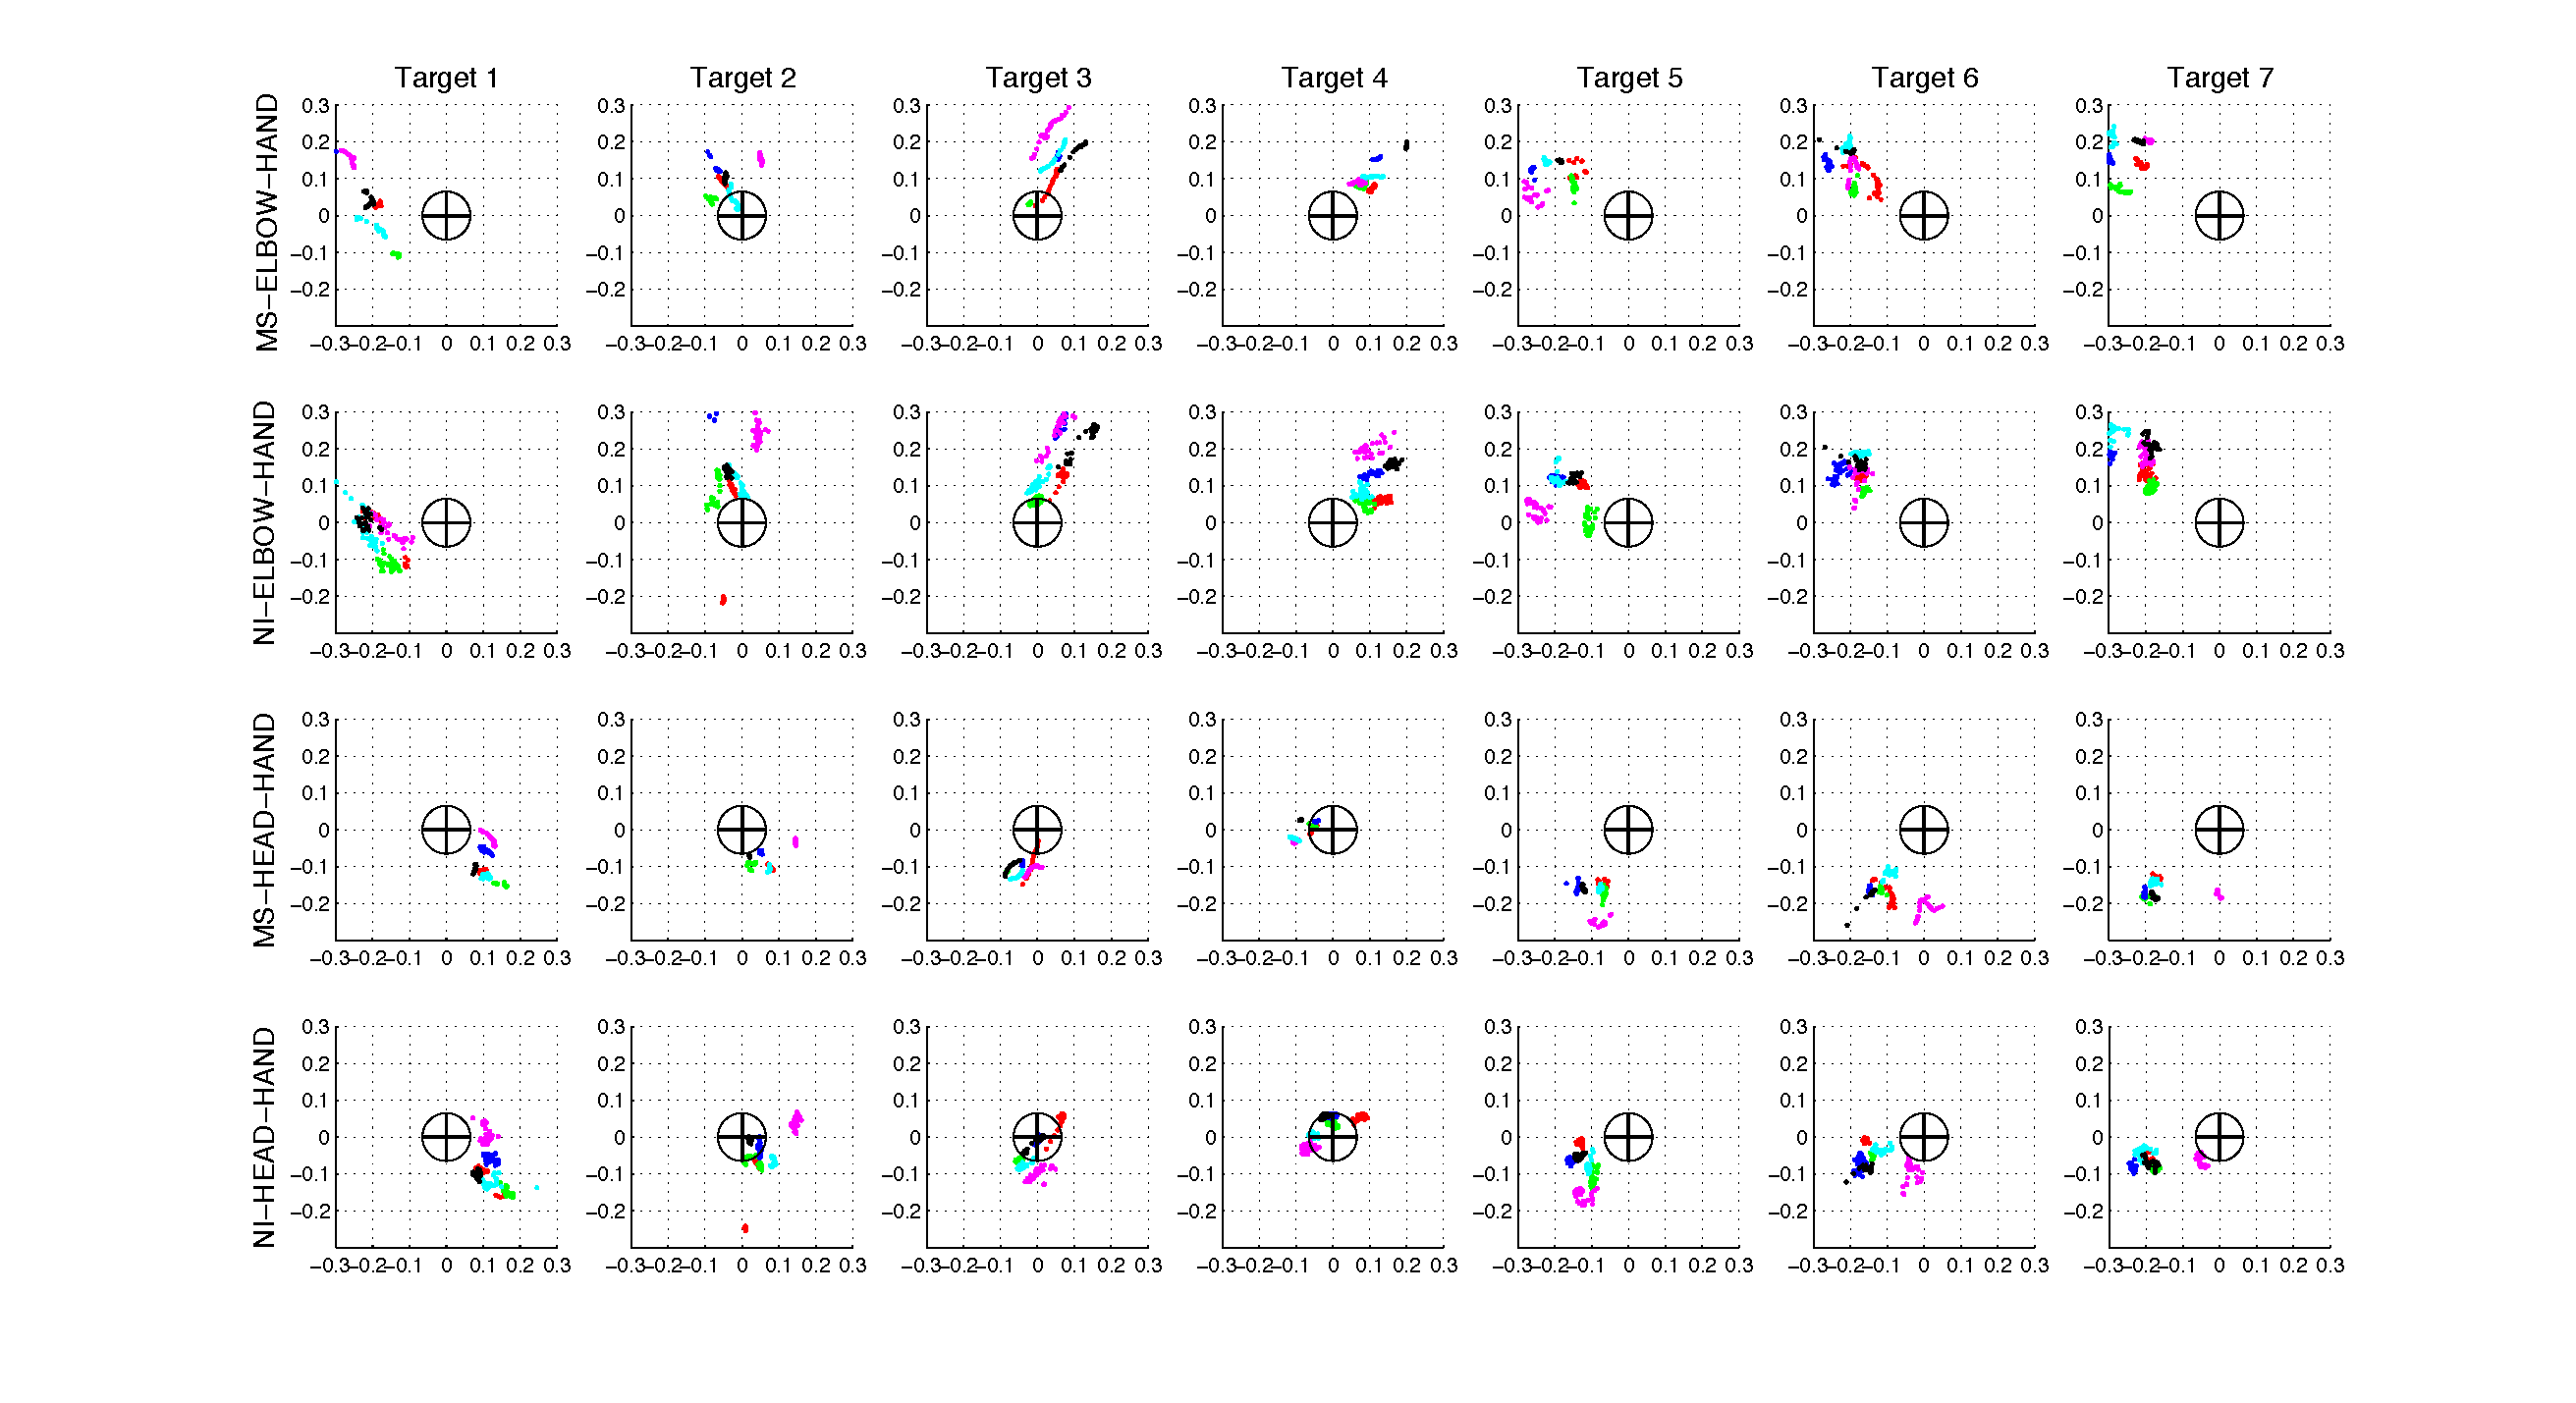
\includegraphics[width=1.5\textwidth]{pics/projections.pdf}
\caption{(Best viewed in color). Euclidean distance error in cartesian coordinates for each gesture method and target. The pointing ray intersection points with the target plane are shown here for each target (T1-T7) as the columns.  Each subject's points are shown in separate colors.  There are 30 points from each subject, corresponding to the 30 frames recorded for the pointing gesture at each target.  Axes are shown in centimeters.  The circle drawn in the center of each plot has the same diameter (13 cm) as the physical target objects used.}
\label{fig:euclidean_projections}
\end{figure*}
\end{landscape}

\begin{landscape}% Landscape page
\begin{center}

\begin{table*}
\centering
\begin{tabular}{c| @{} x{1.0cm}| @{} x{1.0cm}| @{} x{1.0cm}| @{} x{1.0cm}| @{} x{1.0cm}| @{} x{1.0cm}| @{} x{1.0cm}| @{} x{1.0cm}| @{} x{1.0cm}| @{} x{1.0cm}| @{} x{1.0cm}| @{} x{1.0cm}| @{} x{1.0cm}| @{} x{1.0cm}| @{} x{1.0cm}| @{} p{1.0cm}|}
\cline{2-17}
& \multicolumn{4}{c|}{Target 1} & \multicolumn{4}{c|}{Target 2} & \multicolumn{4}{c|}{Target 3} & \multicolumn{4}{c|}{Target 4} \\ \cline{2-17}
& \multicolumn{2}{c|}{$\theta$} & \multicolumn{2}{c|}{$\psi$} & \multicolumn{2}{c|}{$\theta$} & \multicolumn{2}{c|}{$\psi$}  & \multicolumn{2}{c|}{$\theta$} & \multicolumn{2}{c|}{$\psi$}  & \multicolumn{2}{c|}{$\theta$} & \multicolumn{2}{c|}{$\psi$}\\ \cline{2-17}
& \footnotesize{$\mu$} & \footnotesize{$\sigma$} & \footnotesize{$\mu$} & \footnotesize{$\sigma$} & \footnotesize{$\mu$} & \footnotesize{$\sigma$} & \footnotesize{$\mu$} & \footnotesize{$\sigma$} & \footnotesize{$\mu$} & \footnotesize{$\sigma$} & \footnotesize{$\mu$} & \footnotesize{$\sigma$} & \footnotesize{$\mu$} & \footnotesize{$\sigma$} & \footnotesize{$\mu$} & \footnotesize{$\sigma$} \\ \hline
\multicolumn{1}{ |c|}{\textbf{\scriptsize{MS-Elbow-Hand}}}& -15.7 & 2.9  & 5.5 & 6.1  & -4.3 & 6.6  & 7.8 & 3.1  & -3.7 & 2.4  & 7.4     & 3.1  & -3.6 & 1.9  & 11.5 &\multicolumn{1}{r|}{2.9}\\ \hline
\multicolumn{1}{ |c|}{\textbf{\scriptsize{NI-Elbow-Hand}}}& -16.4 & 2.9  & 4.3 & 7.0  &  -3.8 & 6.6  & 11.3 & 10.9  & -4.8 & 2.6  & 9.7 & 3.4  & -4.0 & 4.7  & 12.4 &\multicolumn{1}{r|}{2.5} \\ \hline
\multicolumn{1}{ |c|}{\textbf{\scriptsize{MS-Head-Hand}}}& 7.7 & 2.6  & -12.0 & 5.3  & 10.8 & 6.4  & -9.1 & 3.2  & 2.2 & 2.0 & -8.3   & 3.2  & -4.0 & 1.7  & -4.3 &\multicolumn{1}{r|}{3.2} \\ \hline
\multicolumn{1}{ |c|}{\textbf{\scriptsize{NI-Head-Hand}}}& 8.5 & 2.6 & -11.7 & 6.1  & 10.2 & 6.7  & -5.7 & 8.0  & 2.0 & 2.3  & -2.9    & 4.7  & -3.2 & 2.5  & 1.45 &\multicolumn{1}{r|}{4.8} \\ \hline
\end{tabular}
\caption{$\mu$ and $\sigma$ angular errors in degrees for each of Targets 1-4 (Figure \ref{fig:ground_truth_targets}), for each pointing method. The aggregate $\mu$ and $\sigma$ is also shown.}
\label{table:pointing_horizontal}
\end{table*}

\vspace*{\fill}

\begin{table*}
\centering
\begin{tabular}{c| @{} x{1.0cm}| @{} x{1.0cm}| @{} x{1.0cm}| @{} x{1.0cm}| @{} x{1.0cm}| @{} x{1.0cm}| @{} x{1.0cm}| @{} x{1.0cm}| @{} x{1.0cm}| @{} x{1.0cm}| @{} x{1.0cm}| @{} x{1.0cm}| @{} x{1.0cm}| @{} x{1.0cm}| @{} x{1.0cm}| @{} p{1.0cm}|}
\cline{2-17}
& \multicolumn{4}{c|}{Target 5} & \multicolumn{4}{c|}{Target 6} & \multicolumn{4}{c|}{Target 7} & \multicolumn{4}{c|}{ALL TARGETS} \\ \cline{2-17}
& \multicolumn{2}{c|}{$\theta$} & \multicolumn{2}{c|}{$\psi$} & \multicolumn{2}{c|}{$\theta$} & \multicolumn{2}{c|}{$\psi$}  & \multicolumn{2}{c|}{$\theta$} & \multicolumn{2}{c|}{$\psi$}  & \multicolumn{2}{c|}{$\theta$} & \multicolumn{2}{c|}{$\psi$}\\ \cline{2-17}
& \footnotesize{$\mu$} & \footnotesize{$\sigma$} & \footnotesize{$\mu$} & \footnotesize{$\sigma$} & \footnotesize{$\mu$} & \footnotesize{$\sigma$} & \footnotesize{$\mu$} & \footnotesize{$\sigma$} & \footnotesize{$\mu$} & \footnotesize{$\sigma$} & \footnotesize{$\mu$} & \footnotesize{$\sigma$} & \footnotesize{$\mu$} & \footnotesize{$\sigma$} & \footnotesize{$\mu$} & \footnotesize{$\sigma$} \\ \hline
\multicolumn{1}{ |c|}{\textbf{\scriptsize{MS-Elbow-Hand}}}& -14.5 & 4.1  & 11.6 & 3.7  & -16.6 & 3.3  & 9.9 & 3.7  & -20.8 & 3.7  & 5.7 & 3.4  & -11.3 & 7.7  & 8.5 &\multicolumn{1}{r|}{4.5}\\ \hline
\multicolumn{1}{ |c|}{\textbf{\scriptsize{NI-Elbow-Hand}}}& -12.9 & 4.2  & 9.7 & 5.1  & -16.2 & 2.6  & 11.7 & 3.7  & -20.2 & 4.5  & 8.1 & -3.0  & -11.2 & 7.6  & 9.6 &\multicolumn{1}{r|}{6.3} \\ \hline
\multicolumn{1}{ |c|}{\textbf{\scriptsize{MS-Head-Hand}}}& -9.4 & 1.9  & -11.6 & 3.0  & -7.1 & 4.7  & -13.8 & 1.8  & -8.0 & 5.5 & -15.6 & -2.9  & -1.1 & 8.5  & -10.7 &\multicolumn{1}{r|}{4.8} \\ \hline
\multicolumn{1}{ |c|}{\textbf{\scriptsize{NI-Head-Hand}}}& -11.5 & 1.5 & -4.7 & 4.8  & -11.2 & 4.8  & -4.9 & 2.9  & -12.3 & 5.2  & -8.9 & -2.5  & -2.4 & 9.6  & -5.3 &\multicolumn{1}{r|}{6.4} \\ \hline
\end{tabular}
\caption{$\mu$ and $\sigma$ of angular error in degrees for Targets 5-7 (Figure \ref{fig:ground_truth_targets}), for each pointing method. The aggregate $\mu$ and $\sigma$ is also shown.}
\label{table:pointing_vertical}
\end{table*}

\end{center}
\end{landscape}


\subsubsection{Euclidean error}
\label{sec:pointing_euclidean_error}

Given a ray $\vec{v}$ in the sensors frame from one of the pointing gesture approaches, and a ground truth target point $p_{target}$ lying on a target planar surface, the ray-plane intersection between $\vec{v}$ and plane was computed for each ray, resulting in a 3D point lying on the plane. Figure \ref{fig:euclidean_projections} shows the 2D projections for all 30 measurements from each subject (shown in different colors) and each target. For ease of display, the 3D intersection coordinates with the target planes are displayed in a 2D coordinate system attached to the target plane, with the ground truth target point as the origin.  

As can be seen in Figure \ref{fig:euclidean_projections},  the pointing gesture intersection points were fairly consistent across all users, but varied per target location.  The elbow-hand method produced similar results for MS-SDK and OpenNI. The same is true for the head-hand method.  It is also noteworthy that the data for each target tends to be quite clustered for all methods, and typically not centered on the target location.

\subsubsection{Angular Error}
\label{sec:pointing_angular_error}

We computed the mean and standard deviations of the angular errors in the spherical coordinate system for each pointing gesture method and target. Section \ref{sec:pointing_representing_pointing_directions} describes in detail how the angles $(\theta, \psi)$ are found. The mean and standard deviation values are given in Tables \ref{table:pointing_horizontal} and \ref{table:pointing_vertical}.  The aggregate errors are also displayed as a  box plot in Figure \ref{fig:pointing_angular_boxplots}.

Several observations can be made from these results. The data from the elbow-hand pointing method reports that users typically point about 11 degrees to the left of the intended target direction, and about 9 above the target direction. Similarly, the data from the head-hand pointing method reports that users typically point about 2 degrees to the left of the intended pointing direction, but with a higher standard deviation than the elbow-hand method.  On average, the vertical angle $\psi$ was about 5 degrees below the intended direction for the OpenNI tracker and 10 degrees below for the MS-SDK tracker, with a higher standard deviation than the elbow-hand methods.  The disparity between the two skeleton trackers for this pointing method is because they report different points for the head position, with the MS-SDK head position typically being reported higher than the OpenNI head position. The overall performance of the OpenNI and MS-SDK skeleton trackers, however, is fairly similar, with the MS-SDK having slightly less variation for our dataset.

\begin{figure*}[ht!]%[thpb]
\centering
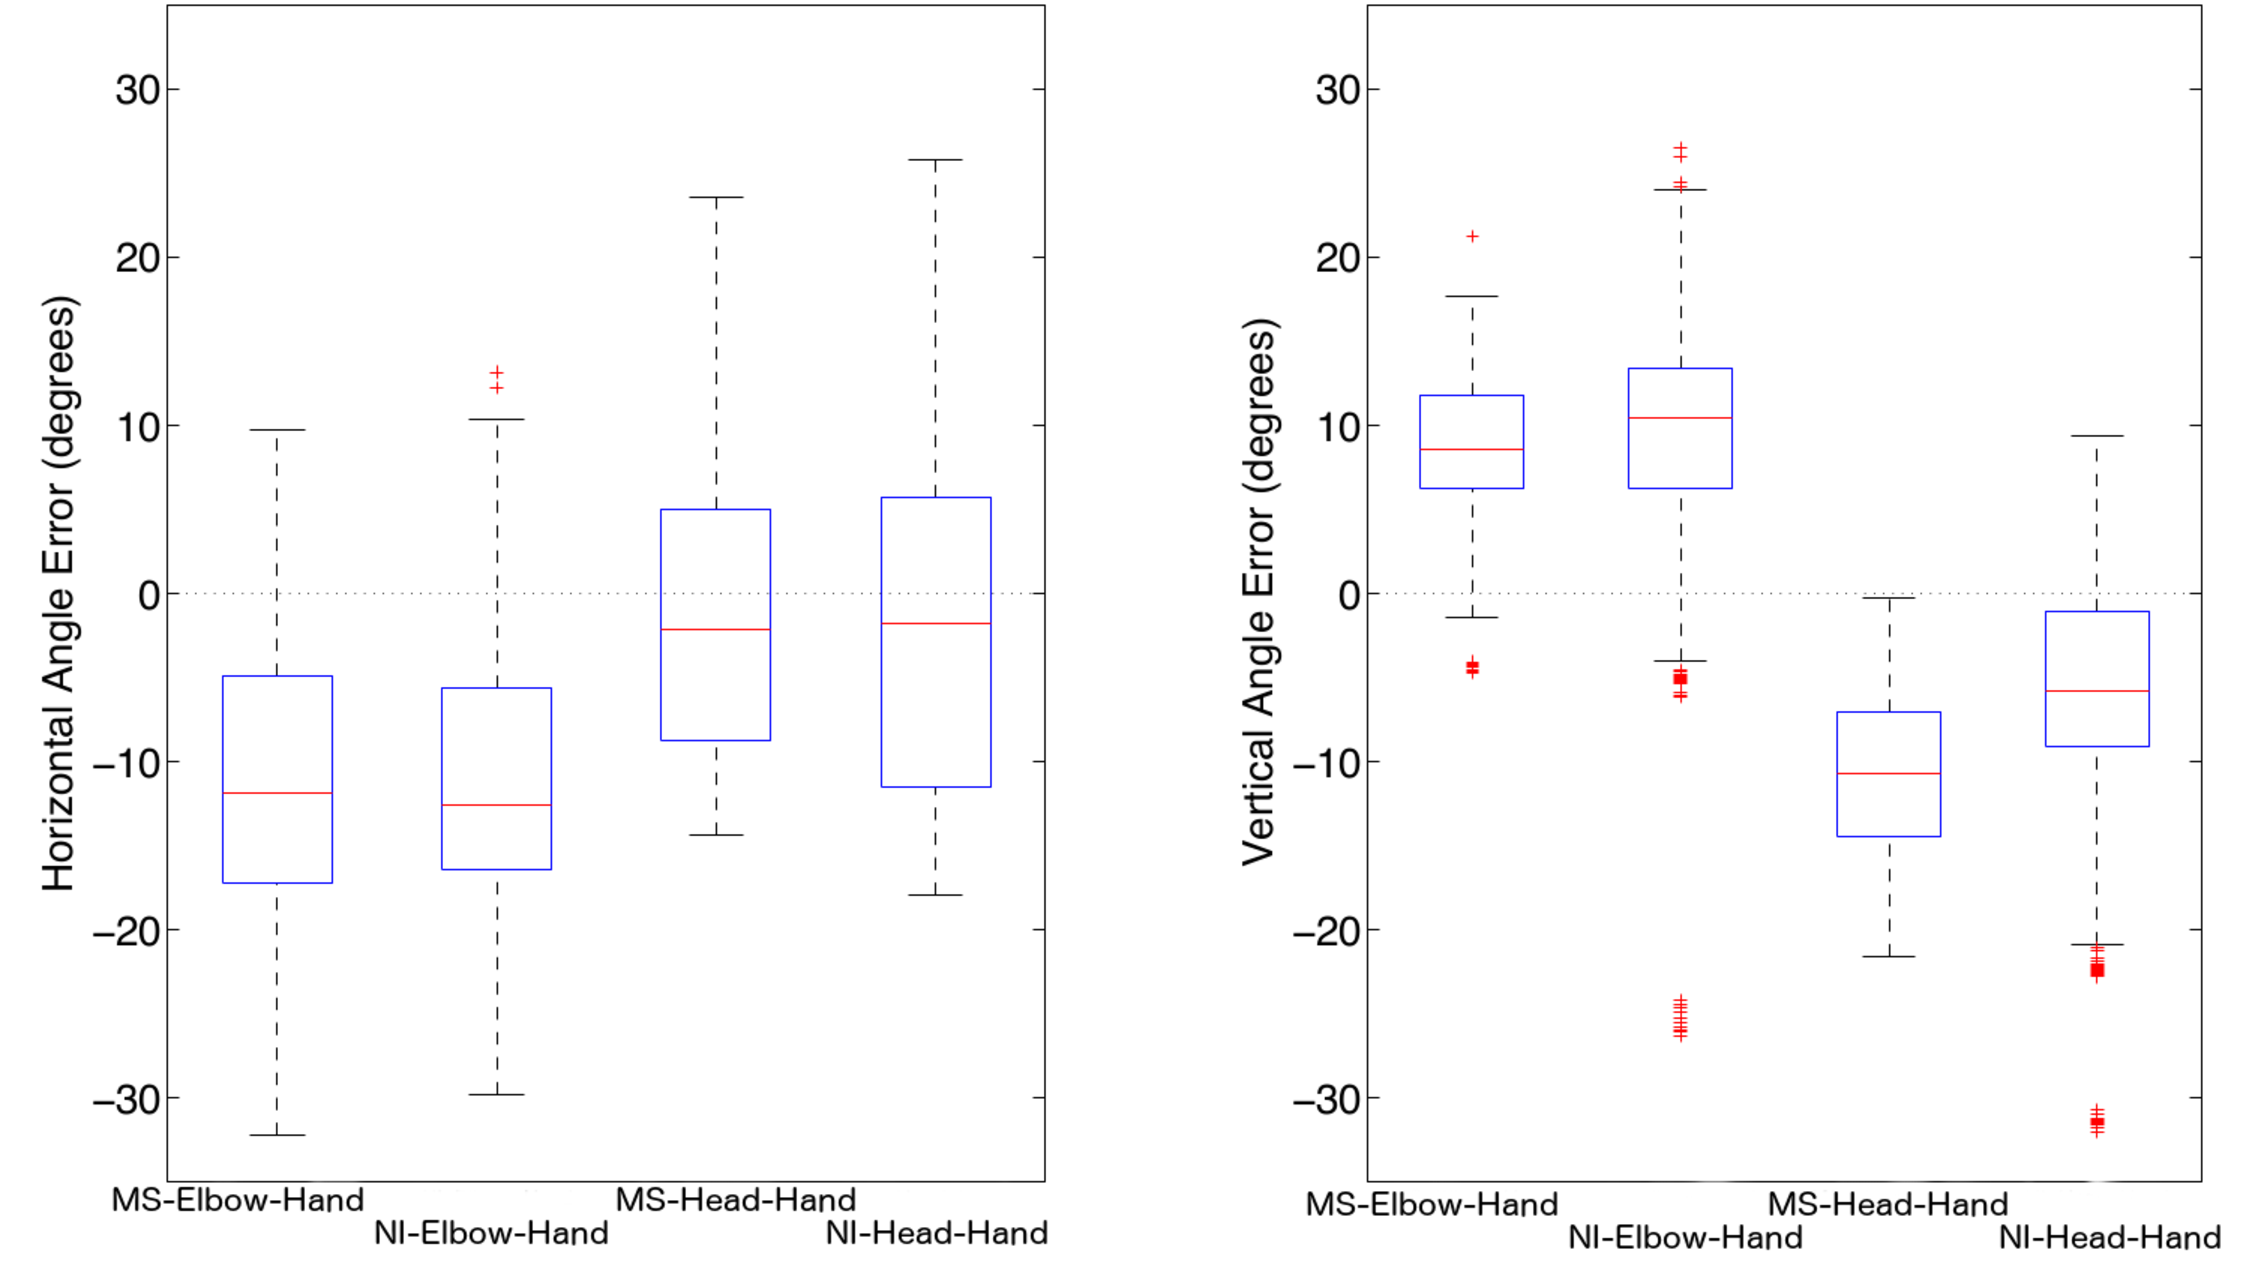
\includegraphics[width=1.0\textwidth]{pics/boxplots_largerfont}
\caption{Box plots of the errors in spherical coordinates $\theta$ and $\psi$ for each pointing method.}
\label{fig:pointing_angular_boxplots}
\end{figure*}

As can be seen in the aggregate box plot in Figure \ref{fig:pointing_angular_boxplots}, the horizontal angle $\theta$ has a higher variation than the vertical angle $\psi$.  Examining the errors for individual target locations shows that this error changes significantly with the target location.  As future work, it would be interesting to collect data for a higher density of target locations to attempt to parameterize any angular correction that might be applied.



\subsection{Object Separation Analysis}

%\subsection{Evaluation}
%\label{sec:pointing_evaluation}

Using the error analysis and pointing gesture model we presented in previous sections, we conducted an experiment to  determine how our approach distinguished two potentially ambiguous pointing target objects. We use the results of the angular error analysis results and not the euclidean error analysis for the remainder of the paper because of our angular representation of pointing gestures.

\begin{figure}[ht!]
\centering
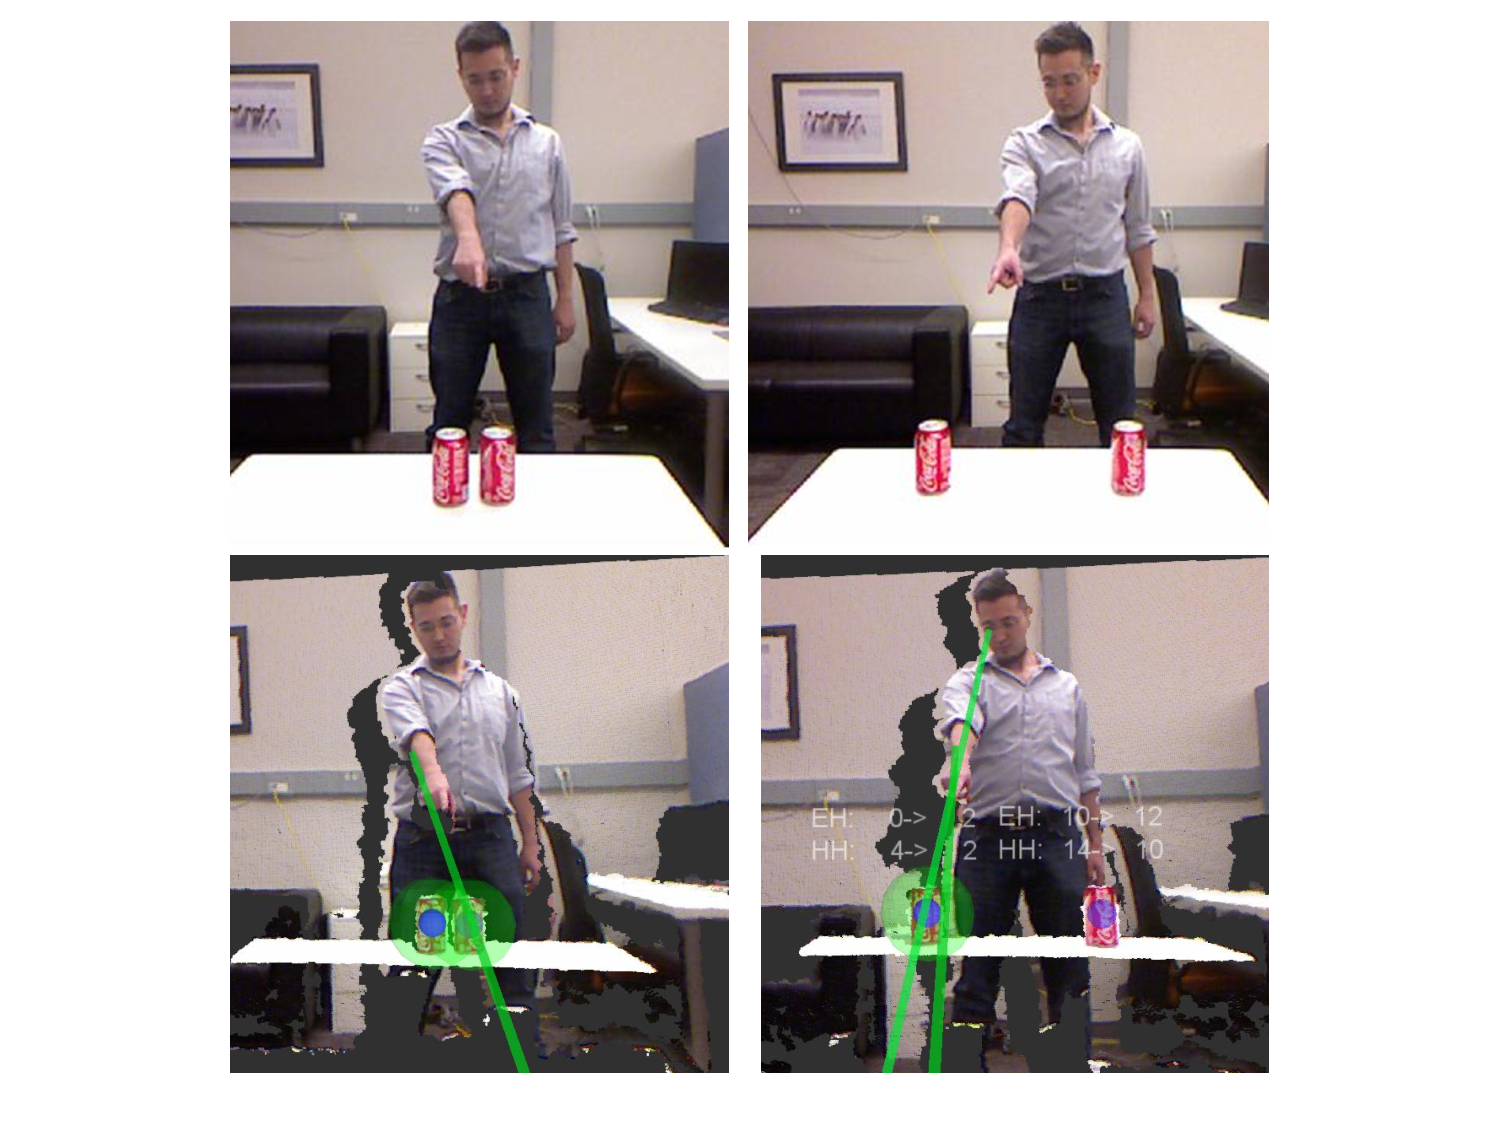
\includegraphics[width=0.75\textwidth]{pics/separation_2_cropped}
\caption{Example scenarios from the object separation test is shown. Our experiments covered separations between 2cm (left images) and 30cm (right images). The object is comfortably distinguished for the 30cm case, whereas the intended target is ambiguous when the targets are 2cm apart. Second row shows the point cloud from Kinect's view. Green lines show the Elbow-Hand and Head-Hand directions whereas green circles show the objects that are within the threshold $D_{mah}<2$.}
\label{fig:pointing_separation}
\end{figure}


The setup consisted of a table between the robot and the person and two coke cans on the table (Figure~\ref{fig:pointing_separation}) where the separation between objects was varied. To detect the table plane and segment out the objects on top of it, we used the segmentation approach presented in~\cite{trevor2013segmentation}. The objects centroid positions, along with their point clouds were calculated in real-time using our segmentation algorithm. The separation between objects were varied with 1 cm increments from $2-15cm$ and with $5cm$ increments between $15-30 cm$. We could not conduct the experiment below 2 cm separation because of the limitations of our perception system. We used the OpenNI skeleton tracker because rest of our system is based in Linux, and we already found that performance difference with MS-SDK for pointing angle errors is insignificant. The experiment was conducted with one user, who was not in the training dataset. For each separation, the user performed 5 pointing gestures to the object on the right and 5 to the object on the left. The person pointed to one of the objects and the Mahalanobis distance $D_{mah}$ to the intended object and the other object is calculated using the approach in Section \ref{sec:pointing_determining_intended_target}. We used the mean and standard deviation values of Target 2 (Figure \ref{fig:ground_truth_targets}) for this experiment because the objects were located between the robot and the person.


\begin{figure*}[ht!]
\centering
%
        \subfigure[]{%
            \label{fig:eh_graph}
            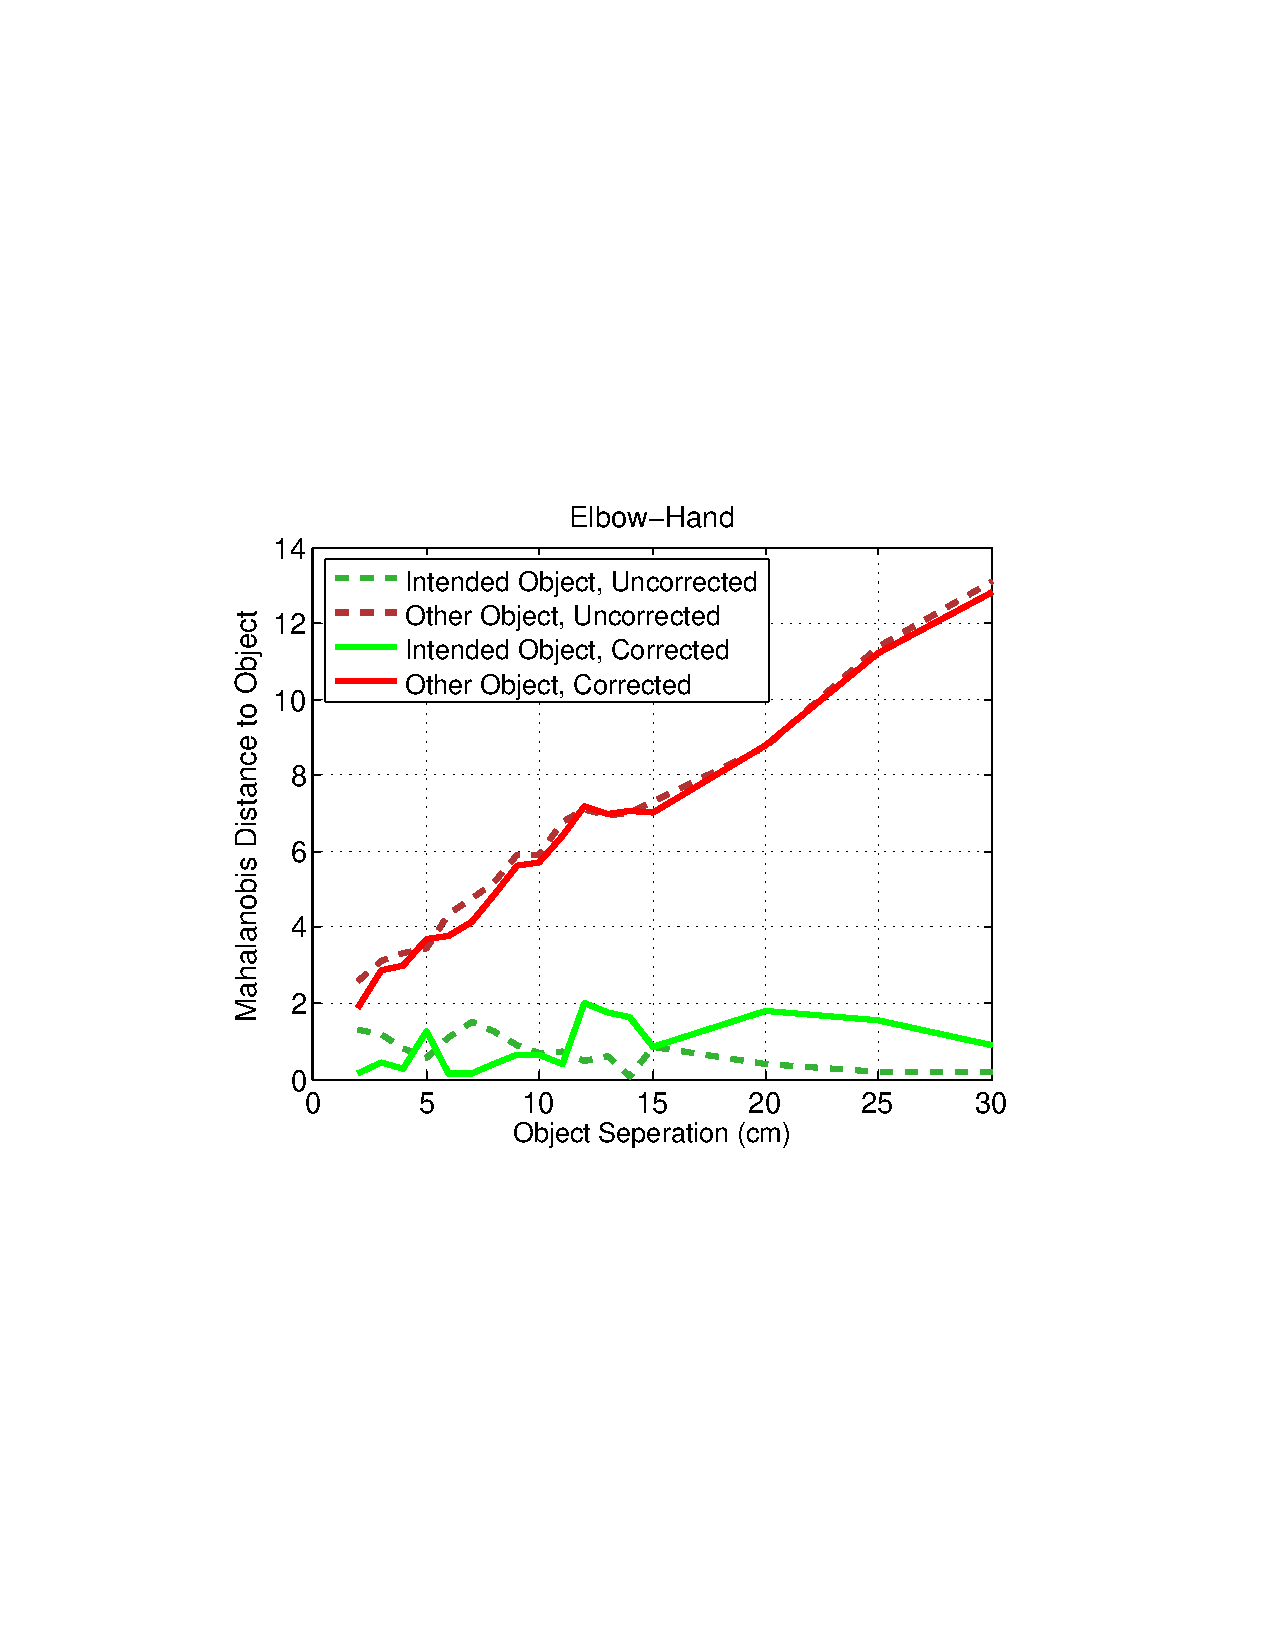
\includegraphics[width=73mm]{pics/eh_graph_crop}
        }%
        \subfigure[]{%
           \label{fig:hh_graph}
           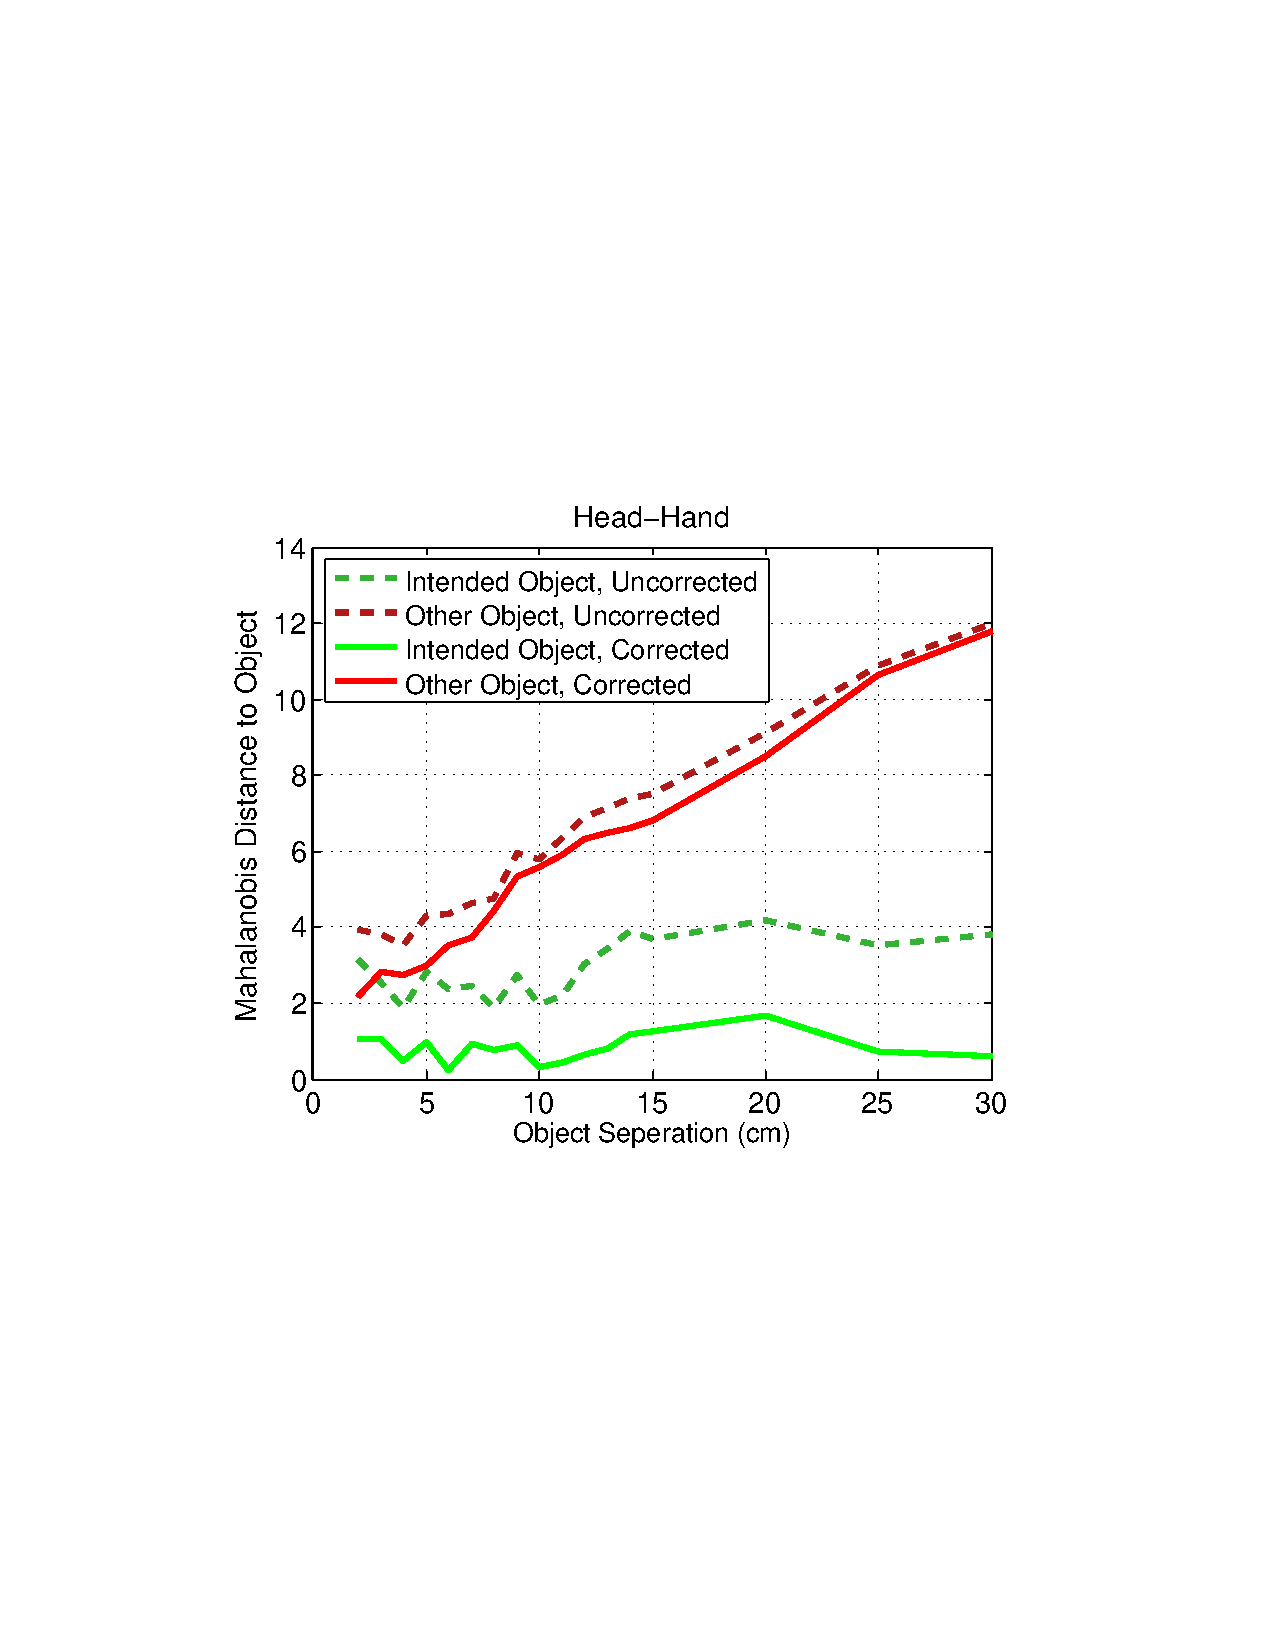
\includegraphics[width=73mm]{pics/hh_graph_crop}
        }        
    \caption{%
	Resulting Mahalanabis distances of pointing targets from the Object Separation Test is shown for a) Elbow-Hand and b) Head-Hand pointing methods. Intended object are shown in green and other object is in red. Solid lines show distances after correction is applied. Less Mahalanobis distance for intended object is better for reducing ambiguity.
     }%
   \label{fig:pointing_graphs}
\end{figure*}

\subsection{Results and Discussion}
\label{sec:results_and_discussion}

The results of the object separation experiment is given for Elbow-Hand (Figure~\ref{fig:eh_graph}) and Head-Hand (Figure~\ref{fig:hh_graph}) methods. The graphs plot object separation versus the Mahalanobis distance for the pointed object and the other object for corrected and uncorrected pointing direction. There are several observations we make by looking at these results.

First, the Mahalanobis distance $D_{mah}$ for the intended object was always lower than the other object. The corrected $D_{mah}$ for both Elbow-Hand and Head-Hand methods for the intended object was always below 2, therefore selecting the threshold $D_{thres}=2$ is a reasonable choice. We notice that some distances for the unintended object at $2cm$ separation is also below $D_{mah}<2$. Therefore, when the objects are $2 cm$ apart, then the pointing target becomes ambiguous for this setup. For separations of $3cm$ or more, $D_{mah}$ of the unintended object is always over the threshold, therefore there is no ambiguity.

Second, correction significantly improved Head-Hand accuracy at all separations, slightly improved Elbow-Hand between $2-12cm$ but slightly worsened Elbow-Hand after $12cm$. We attribute this to the fact that the angles we receive is heavily user-dependent and can have a significant variance across methods as showed in Figure~\ref{fig:pointing_angular_boxplots}. Moreover, the user was not in the training set.

Third, the Mahalanobis distance stayed generally constant for the intended object, which was expected. It linearly increased with separation distance for the other object.

Fourth, patterns for both methods are fairly similar to each other, other than Head-Hand uncorrected distances being higher than Elbow-Hand.

\subsection{Conclusions}
\label{sec:pointing_conclusions}

Humans and robots engaged in joint actions that involve objects will need to be able to communicate about these objects. Deictic gestures can play a crucial part such communication, especially when establishing goals and negotiating responsibilities. A pointing target detection approach that returns a single hypothesis can lead to failures due to perception error. On the other hand, estimation of a pointing likelihood of nearby objects can give valuable insight to a robot. For example, a robot can ask the user to disambiguate the objects if it perceives more than one object that has a significant likelihood of being referred to.

In this work, we model the uncertainty of pointing gestures in a spherical coordinate system, use this model to determine the correct pointing target, and detect when there is ambiguity. Two pointing methods are evaluated using two skeleton tracking algorithms: Elbow-Hand and Head-Hand rays, using both OpenNI NITE and Microsoft Kinect SDK.  A data collection with 6 users and 7 pointing targets was performed, and the data was used to model users pointing behavior.  The resulting model was evaluated for its ability to distinguish between potential pointing targets, and to detect when the target is ambiguous. Our evaluation showed that in a scenario where the separation between two objects were varied, our system was able to identify that there is ambiguity for 2 cm separation and comfortably distinguished the intended object for 3 cm or more separation.


%%%%%%%%%%%%%%%%%%%%%%%%%%%%%%%%%%%%%%%%%%%%%%%%%%%%%%%%%%%%%%%%%%%%%%

\chapter{Navigation Among People}
\label{chapter:navigation_among_people}

Autonomous navigation is one of the most fundamental tasks for a mobile robot. For a mobile robot with adequate actuation and sensing, collision-free navigation is considered a solved problem. There are many algorithms that achieve point-to-point autonomous navigation thanks to the advances in the motion planning community. Many of these algorithms are optimized to find the least-cost path, or the shortest path. However, when there are humans in the environment, such algorithms suddenly become inefficient or insufficient. For example, while it is acceptable for a robot to get inches close to a wall, doing so to a human is socially unacceptable and potentially dangerous. Similarly, sudden appearance of a robot can surprise or shock humans. There are many other social scenarios where the shortest path may not be optimal. 

In addition to sub-optimality, these approaches may be incomplete in the sense that they can not find a solution even though there is a feasible one. This is because shortest-path navigation algorithms treat every object in the environment as an obstacle. This assumption does not hold when intelligent agents are present in the environment. Therefore navigation should differentiate humans and obstacles for more intelligent robot behavior.

Another aspect to spatial interaction between humans and robots is the dynamics of the robot motion. For example, people may feel uncomfortable and unsafe when they are in close proximity to high-speed agents or objects. Therefore, for a robot in a human environment, while it may be acceptable to speed up in dedicated regions, its speed should be limited in places where there is a significant possibility of encountering a human.

In this Chapter, we first provide a background and present the most common approach in contemporary autonomous navigation methods in Section \ref{sec:navigation_contemporary_navigation_practices}. Second, we provide provide relevant works on navigation among people in Section \ref{sec:navigation_related_work}. Third, in Section \ref{sec:navigation_finding_goal_points_for_navigation}, we present how the goal points for navigation are determined. We then present our people-aware navigation method in Section \ref{sec:navigation_people_aware_navigation}. Lastly, we touch to the subject of introducing speed limits for all robots in a human environment in Section \ref{sec:navigation_speed_limits}.


\section{State-of-the-Art Approach in Autonomous Navigation}
\label{sec:navigation_contemporary_navigation_practices}

There are two prerequisites that enables autonomous navigation: 

\begin{enumerate}
\item The map of the environment, usually in the form of a discrete grid, that represents static objects in the environment
\item A way to localize the robot in the map using sensory information as it moves in the environment
\end{enumerate}

Robot navigation involves finding a collision-free path from a start pose $(x_{0},y_{0},\theta_0)$ to a goal pose $(x_{g},y_{g},\theta_g)$. In real-time operation, $(x_{0},y_{0}, \theta_0)$ is the robot's current pose as the robot tries to reach to the goal pose from where it currently is. $\theta_g$ is optional as the goal of the robot could be to reach the goal position regardless of its orientation. The goal position is provided from an external process, and we will touch upon how the goal positions are calculated in Section \ref{sec:navigation_finding_goal_points_for_navigation}.



\begin{figure}[ht!]
\centering
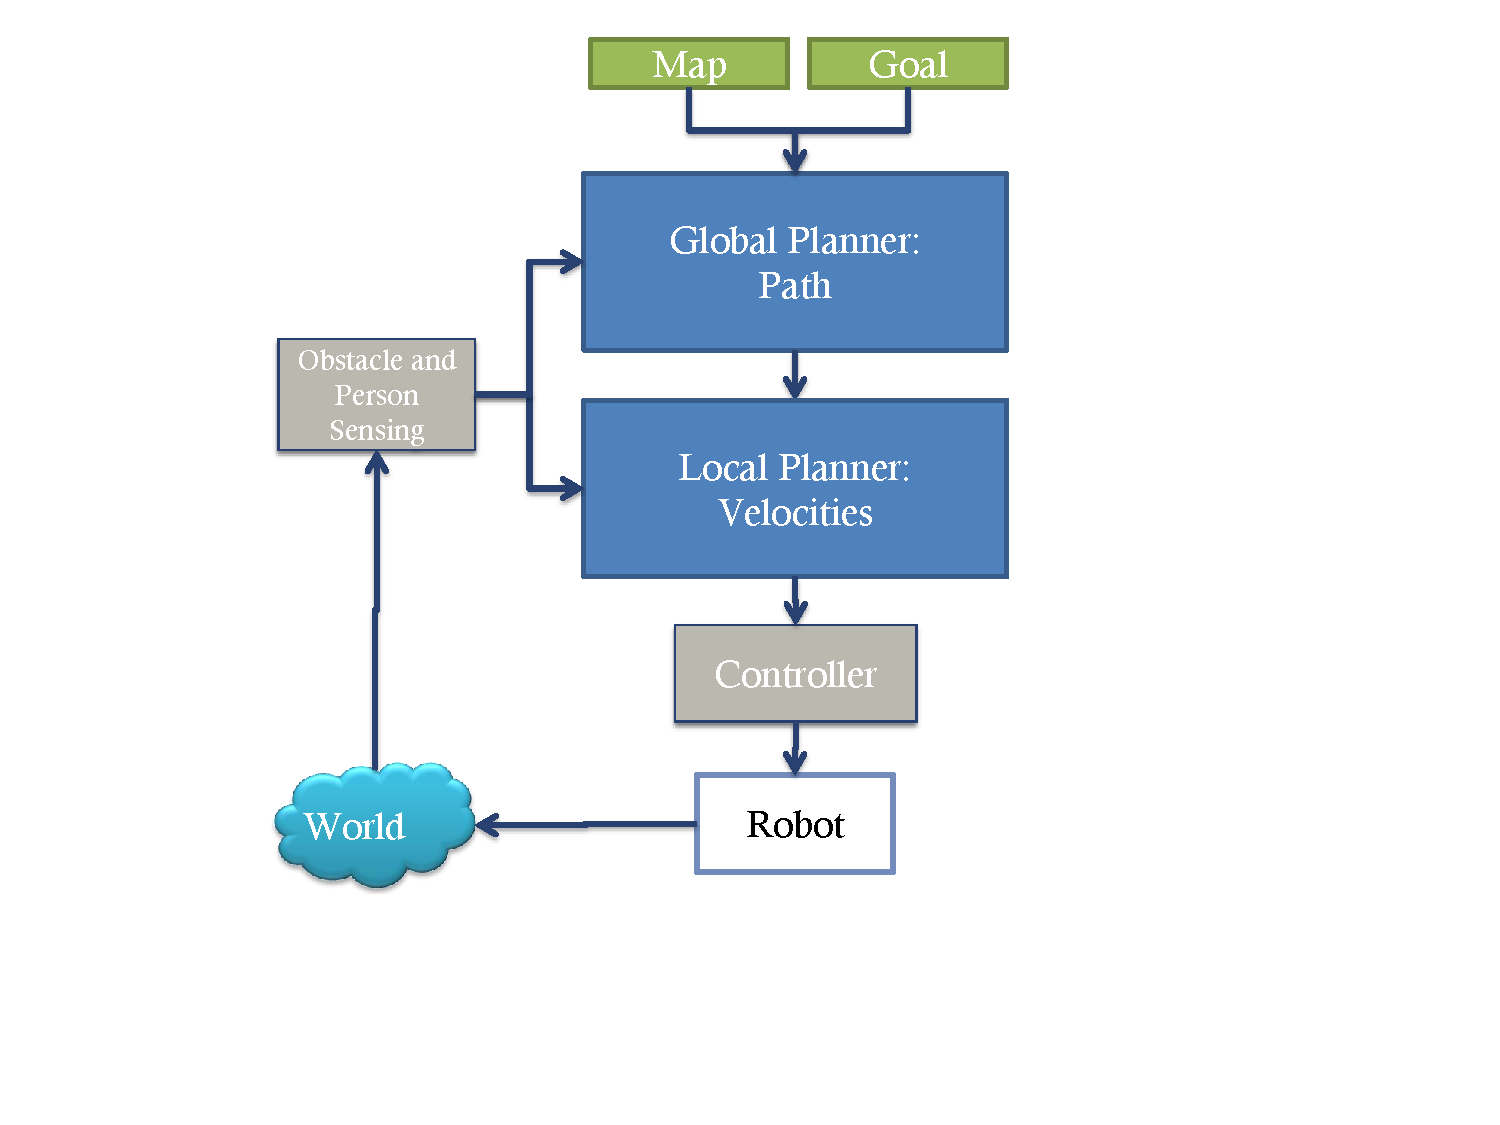
\includegraphics[width=0.5\textwidth]{pics/navigation_overview}
\caption{High-level system overview of mobile robot navigation}
\label{fig:navigation_overview}
\end{figure}

A common approach to path planning is to divide the path planning into two parts: $global$ and $local$. Global planning aims to find a path from the start position to the goal position. The global path is a set of consecutive positions that connect the start to goal position. A global path is usually found with a search algorithm executed on a graph of points. The search heuristics is dependent on specific global planners, and in most cases collision-free shorter paths are favored. The local planner is responsible to execute the global path by calculating a trajectory and sending velocity commands to motor controllers. As the robot acts in the environment, its sensors sense the new state of the robot and people, and the new iteration begins. This cycle is shown in Figure \ref{fig:navigation_overview}. 

A popular method to to implement the global and local planners is by using a $costmap$. A $costmap$ not only has the same representation as the map, however collision-free positions can have non-zero costs. A lower cost cell is more favored to be in to a higher cost cell. After the calculation of all cells, the least-cost path is found that connects the start position to the goal position.

Note that this approach assumes the robot is able to execute any path provided to it. Holonomic robots can move in any direction, however non-holonomic robots has limitations in their movements. For example, two wheel robots can not move sideways. Two common approaches to solve this problem are: to implement trajectory planners that can handle imperfect control or to embed the robot's dynamics into sampling for global and local planning.

\section{Related Work}
\label{sec:navigation_related_work}

In this section, we review the literature on robot navigation in human environments including socially acceptable navigation, learning behaviors from humans and cooperative navigation.

\subsection{Socially Acceptable Path Planning}
Socially acceptable robot navigation is considered in different applications such as free navigation~\cite{sisbot2007human}, approaching people~\cite{satake2009approach} and evacuating buildings~\cite{ohki2010collision}. Some works used the personal space concept in cost-based general path planners~\cite{sisbot2007human,kirby2009companion}. Sisbot~\cite{sisbot2007human} models the social spaces as a ellipse-shaped Gaussian, and takes into account the safety, preferences and vision fields of humans for a robot that navigates from a location to another. Kirby~\cite{kirby2009companion} presents a path planner that takes into account social conventions such as tending to one side of the hallways. A potential field based trajectory planner for dynamic human environments is presented by Svenstrup~\cite{svenstrup2010trajectory}. Rios-Martinez~\cite{rios2011understanding} presents a RRT-based planner that considers not just safety but also the disturbance of humans. In simulation, if interaction within a group of people is detected, the robot can either not disturb the interaction or join the group. This approach is implemented on a wheelchair robot~\cite{vasquez2012human}. Althaus~\cite{althaus2004navigation} presents a robot that can join a group of people and adjust to the formation reactively. The scenario where a robot encounters a human in a hallway is studied by Pacchierotti ~\cite{pacchierotti2005human}. Parameters such as the distance between the human and the robot when the robot begins to deviate from its path and lateral distance that robot should be placed when it is passing the human are found from experiments. Recent work by Lu~\cite{lu2013towards} showed that using gaze cues and social navigation makes robot-human hallway passing more efficient.

\subsection{Learning Navigation from Human Behavior}

Behaving human-like in robot navigation is usually favored in the literature~\cite{sasaki2006human}. One way to simulate human navigation behavior is to use social cost maps that capture social conventions \cite{scandolo2011anthropomorphic,luber2012socially}. Contrary to the imitation approach, \cite{bennewitz2005learning} tries to avoid predicted paths, with the goal to minimize the risk of interference. Kuderer~\cite{kuderer2013teaching} presents a tele-operated robot that computes the policy of a desired interactive navigation by learning from observations of pedestrians. Pellegrini~\cite{pellegrini2009you} trains a dynamic social behavior, that account for social interactions, using pedestrian data.

\subsection{Human Cooperation in Robot Navigation}

Robots can exploit human cooperation in certain scenarios. In populated environments, one way to move with the crowd is to follow individuals that move towards the robot's goal~\cite{stein2012robot,muller2008socially}. 

Some of the recent works in the literature claim that the robot motions should be predictable so the human observers can judge the motive and future behavior of the robot. Observational study in~\cite{lichtenthaler2013towards} claims that three features can increase the predictability of robot navigation: straight lines, stereotypical motions and usage of additional gestures. In a user study conducted by Gockley~\cite{gockley2007natural}, humans observers watched two ways of person following. People found direction-following more natural than exact path following. Kruse~\cite{kruse2012legible} observes that when paths of two humans are crossed at a right angle, they adapt their velocity rather than the path. This behavior is implemented on a robot, resulting in more predictable motions. 

Trautman~\cite{trautman2010unfreezing} introduces the 'freezing problem', where traditional path planners fail to produce a feasible solution in crowded human environments. Muller~\cite{muller2008socially} briefly mentions a 'shooing away' behavior, where the robot accelerates towards a human, hoping that he/she will get out of the way. Kruse~\cite{kruse2010exploiting} introduces an optimistic planner, which assumes that people will cooperate with robot movements. Their approach relies on assigning a non-infinite cost if a robot enters to a human's personal space, however the plan fails if humans doesn't move as expected because of the lack a local planner.

\section{Mapping and Localization}
\label{sec:mapping_localization}

Our system uses a 2-layer map:

\begin{enumerate}
\item Metric layer: Used for localization and obstacle avoidance
\item Semantic layer: Includes features such as planar landmarks, doors, navigation waypoints and objects
\end{enumerate}

In a new environment, we first run the ROS $gmapping$ Simultaneous Localization and Mapping (SLAM) package to generate the metric map. This SLAM approach is based on Rao-Blackwellized particle filter \cite{grisetti2007improved}. The front Hokuyo laser scanner at ankle level is used as the main sensor to generate the map and to localize the robot. The semantic layer is be generated by the interactive Tour Scenario (Chapter \ref{chapter:map_annotation}) and edited using the interactive Tour Scenario.

After the map is generated and saved, we localization only using this map. ROS $amcl$ package is used for localization, which implements the KLD-samping Monte Carlo particle localization approach \cite{fox1999monte}. This localization system is a local localization system, meaning it only can estimate the position of the robot given past location information. Therefore, when the robot is started, this method of localization needs a global position estimate. We offer two methods of initialization.

\begin{enumerate}
\item Manual Initialization: This is the standard method of initialization in ROS. The robot programmer provides a crude estimate to the system by clicking to a point in the map, using robot's computer.
\item Automatic Initialization using QR codes: We use a specially designed and located QR code to automatically localize the robot the first time.
\end{enumerate}

The first initialization method, in its current form, requires a robotics expert to specify the initial pose of the robot. We present our QR code based automatic initialization method here. The QR code includes links to the map and landmarks, speed limits, as well as the location of the QR pattern in the map. Therefore the robot automatically can infer its initial location upon detection of the QR code, without external intervention. System designers place QR code tags to the environment to a couple of strategic places. These places can be walls at the entrance of an indoor space, or mostly visited areas. QR codes in general contain links, text and various other data. In our application, the QR pattern includes text in XML format, which includes the link to the map and speed map files, and the position of the QR pattern in the map. Here is a sample information that a robot can read from a QR pattern:


\begin{figure}[ht!]
\centering
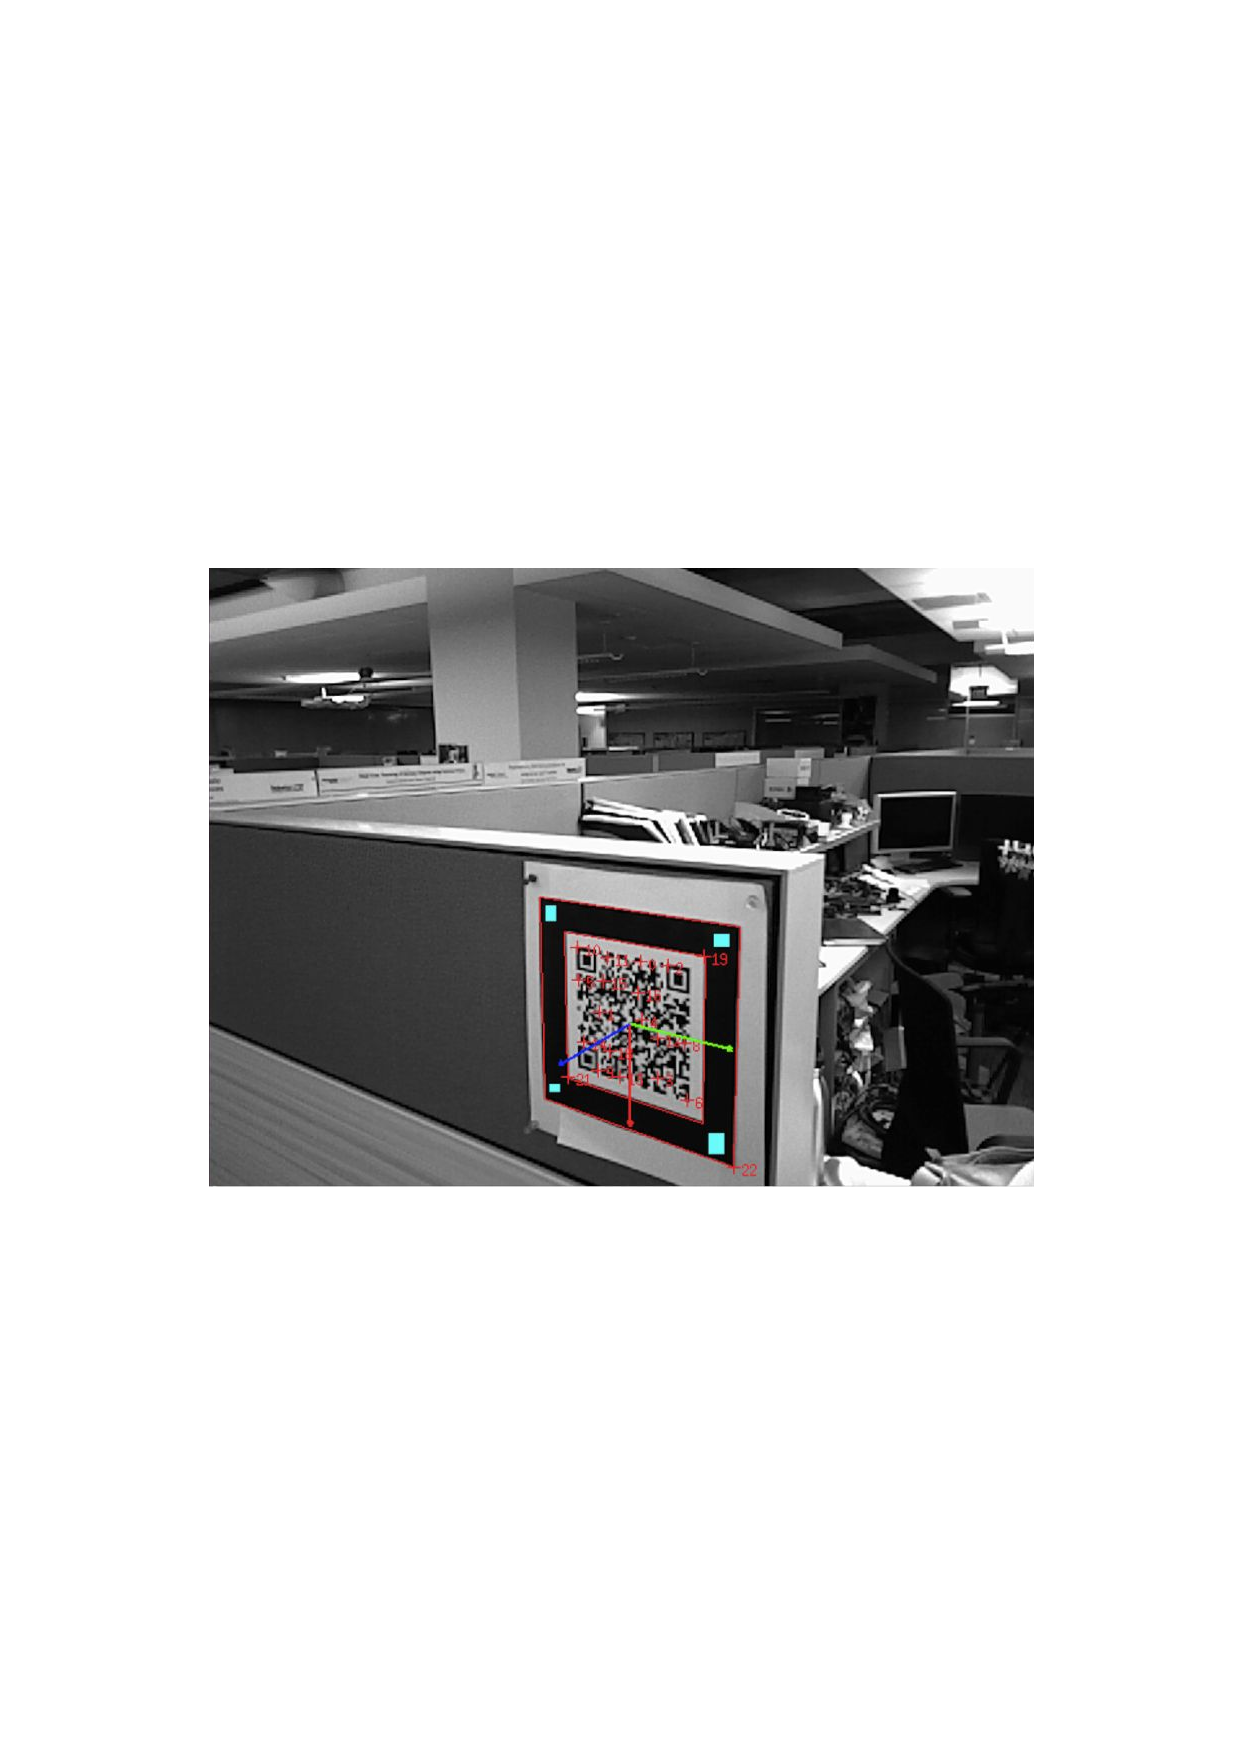
\includegraphics[width=0.6\textwidth]{pics/qrcode}
\caption{A robot can acquire map information and localize itself against the map upon detection of a specially designed QR code}
\label{fig:qr}
\end{figure}

\begin{lstlisting}
<root>
  <map>http://link1/</map>
  <speedmap>http://link2/</speedmap>
  <x>101.26</x>
  <y>98.76</y>
  <z>1.45</z>
  <q1>0.0</q1>
  <q2>0.0</q2>
  <q3>0.0</q3>
  <q4>1.0</q4>
</root>
\end{lstlisting}


The position provided in the pattern is the position and orientation (in quaternions) of the QR tag in the map frame. Using this information, a robot can acquire the knowledge of the environment automatically and locate itself in the map, where:

$^{robot}T_{cam}$ is the transformation from the robot base frame to the camera frame on the robot and is known.

$^{cam}T_{QR}$ is the pose of the QR code in the camera frame and is available upon detection of the QR code.

$^{map}T_{QR}$ is the transformation from the robot base frame to the camera frame on the robot and is read from the data embedded to the QR code.

$^{map}T_{robot}$ is the pose of the robot in the map and is unknown.\\

$^{map}T_{robot}=(^{map}T_{QR})*(^{QR}T_{robot})$

$^{QR}T_{robot}=(^{QR}T_{cam})*(^{cam}T_{robot})=(^{cam}T_{QR})^{-1} * (^{robot}T_{cam})^{-1}$

Therefore:

$^{map}T_{robot}=(^{map}T_{QR})*(^{cam}T_{QR})^{-1} * (^{robot}T_{cam})^{-1}$\\



$(x,y,\theta)$ of the robot in the map frame is required for initialization. $x$ and $y$ is readily found by looking at the displacement of the transformation. $\theta$ is found by projecting the axes to the map floor plane and . After the initial pose is provided, \textit{amcl} package handles the localization using the laser scanner readings.

We used the \textit{visp\_auto\_tracker} ROS package to extract the pose of the QR code and the content embedded in the pattern. To interpret the XML data, we used libXML++ package.


\section{Goal Points for Navigation}
\label{sec:navigation_finding_goal_points_for_navigation}

As presented in Section \ref{chapter:map_annotation}, our interactive system allows a user to annotate landmarks. After completing the $Home Tour$, the robot can navigate to or towards the labeled entities.
A user can enter a navigation destination to the robot in three distinct ways: via labeled waypoints, planar landmarks or objects.

\subsection{Labeled Waypoints:} If a waypoint is labeled and saved, the robot attaches that label to the explicit coordinates, namely position and orientation. Therefore, if the robot is instructed to navigate to a labeled waypoint, then the goal is readily the pose of the waypoint.
\subsection{Labeled Planar Landmarks:} If the label is attached to planar landmark, or a set of planar landmarks, we use the following methodology depending on the number of landmarks attached to the corresponding label:

\subsubsection{Only a single plane has the corresponding label: }
\label{sec:navigation_goal_single_label}

\begin{figure}[ht!]
\centering
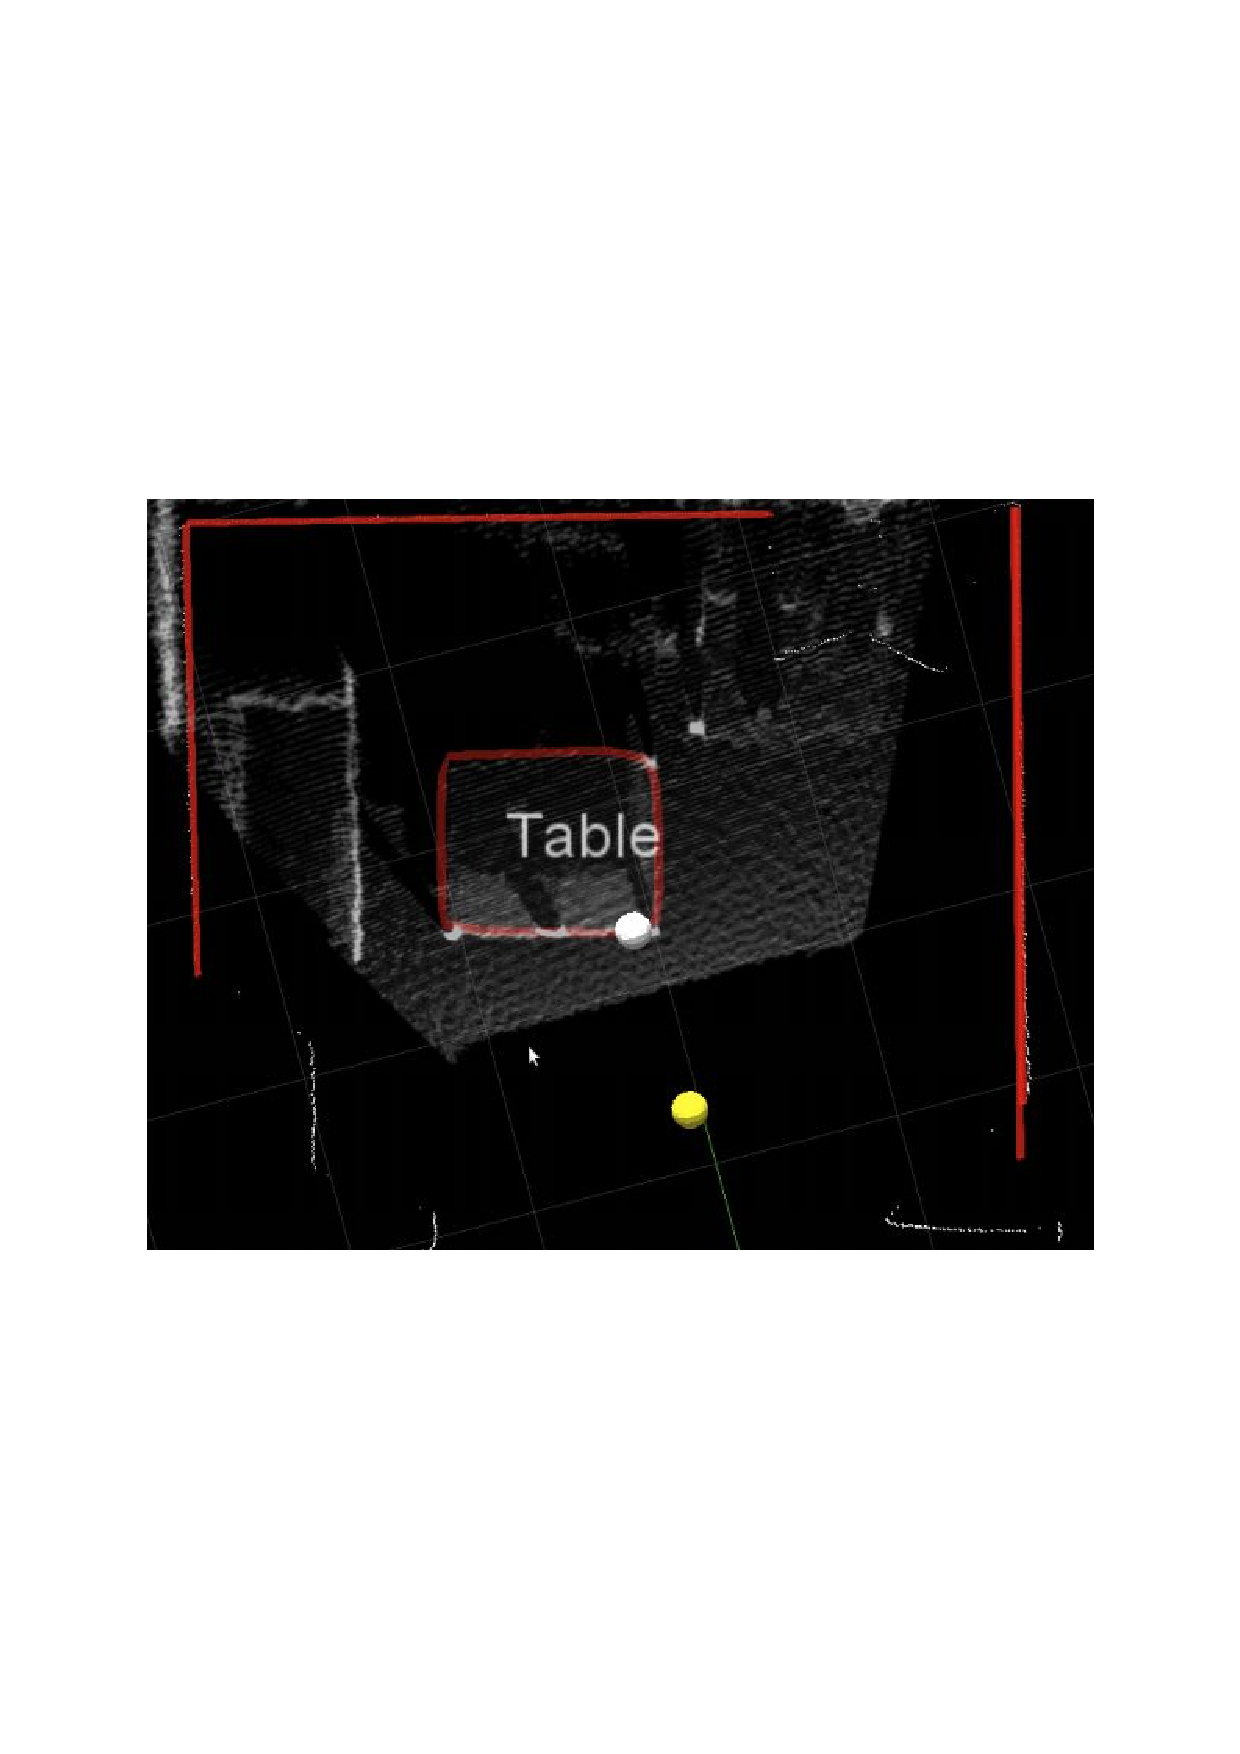
\includegraphics[width=0.6\textwidth]{pics/single_plane}
\caption{Top down point cloud view of a room. A planar landmark with label $Table$ has previously been annotated by a user. The convex hull for the planar landmark is shown in red lines. When asked to navigate to $Table$, the robot calculates a goal pose, which is shown as the yellow point.}
\label{fig:single_plane}
\end{figure}

We assume that the robot should navigate to the closest edge of the plane, so we select the closest vertex on the landmark's boundary to the robot's current position. This point is projected down to the ground plane, as our robot navigates on the floor. We calculate a line between this point and the robot's current pose, and navigate to a point on this line a meter away from the point, and facing this point. This results in the robot navigating to near the desired landmark, and facing it. This method is suitable for both horizontal planes such as tables, or vertical planes such as doors. An example for calculating a goal for a single labeled planar landmark is shown in Figure \ref{fig:single_plane}. 

where a the goal point corresponding to the singular label $Table$. 

\subsubsection{Multiple planes are attached to the same label: }

\begin{figure}[ht!]
\centering
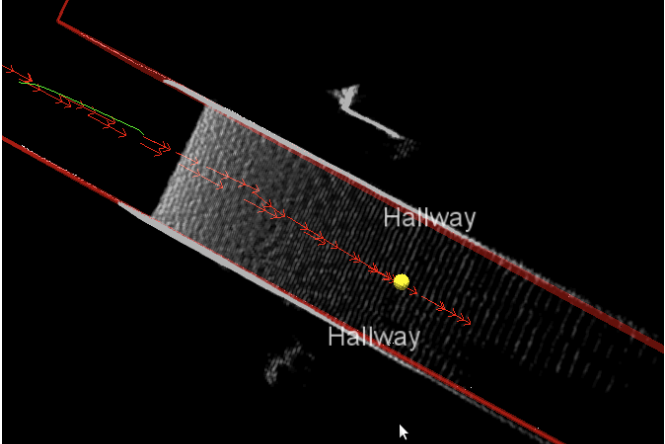
\includegraphics[width=0.65\textwidth]{pics/double_plane}
\caption{Top down point cloud view of a hallway. The user has previously annotated two planar landmarks with the same label, $Hallway$. When asked to navigate to $Hallway$, the robot calculates a goal pose, which is shown as the yellow point.}
\label{fig:double_plane}
\end{figure}

We assume that the requested label corresponds to a region of space such as a room or corridor. In this case, we project the points of all planes with this label to the ground plane, and compute the convex hull. For the purposes of navigating to this label, we simply navigate to the centroid of the hull. While navigating to a labeled region is a simple task, this labeled region could also be helpful in the context of more complex tasks, such as specifying a finite region of the map for an object search task. An example for calculating a goal for a two labeled planar landmarks is shown in Figure \ref{fig:double_plane}. 


\subsection{Labeled Objects:} As discussed in Section \ref{sec:map_objects}, we first perform planar surface detection before detecting tabletop objects. When the robot is asked to navigate to a labeled object, the planar surface that the object lies on is given as the goal landmark. The robot calculates the goal position as described in the single labeled landmark case in Section \ref{sec:navigation_goal_single_label}.

\section{People Aware Navigation}
\label{sec:navigation_people_aware_navigation}

A extensively reviewed in Section \ref{sec:navigation_related_work}, people-aware navigation algorithms aim to generate human-friendly paths that consider the safety and comfort of people. A common assumption for point-to-point people aware navigation is that humans are independent agents and that robot's motions have no effect on people's motions. However, humans navigate by constantly anticipating other people's reactions. Similarly, mere presence of a robot in motion is likely to influence how nearby humans would move. 

Robots can potentially use this implicit cooperation between moving embodied agents. For example, consider a robot that is outside a room and given a goal pose in the room. There is a person standing at the door and blocking the path. Such an example is illustrated in Figure \ref{fig:room}. Standard path planners, as well as planners that consider dynamic objects fail to produce a solution to this problem. The role of physical embodiment in human-robot interaction is significant~\cite{wainer2006role}, however it is commonly ignored in robot navigation. A people-aware planner should anticipate that the human may give way to the robot if it expresses its intent to go inside the room. Extending this idea, by using anticipation a robot can reduce its time of travel and behave more human-like in general cases.

\begin{figure}[t!]
\centering
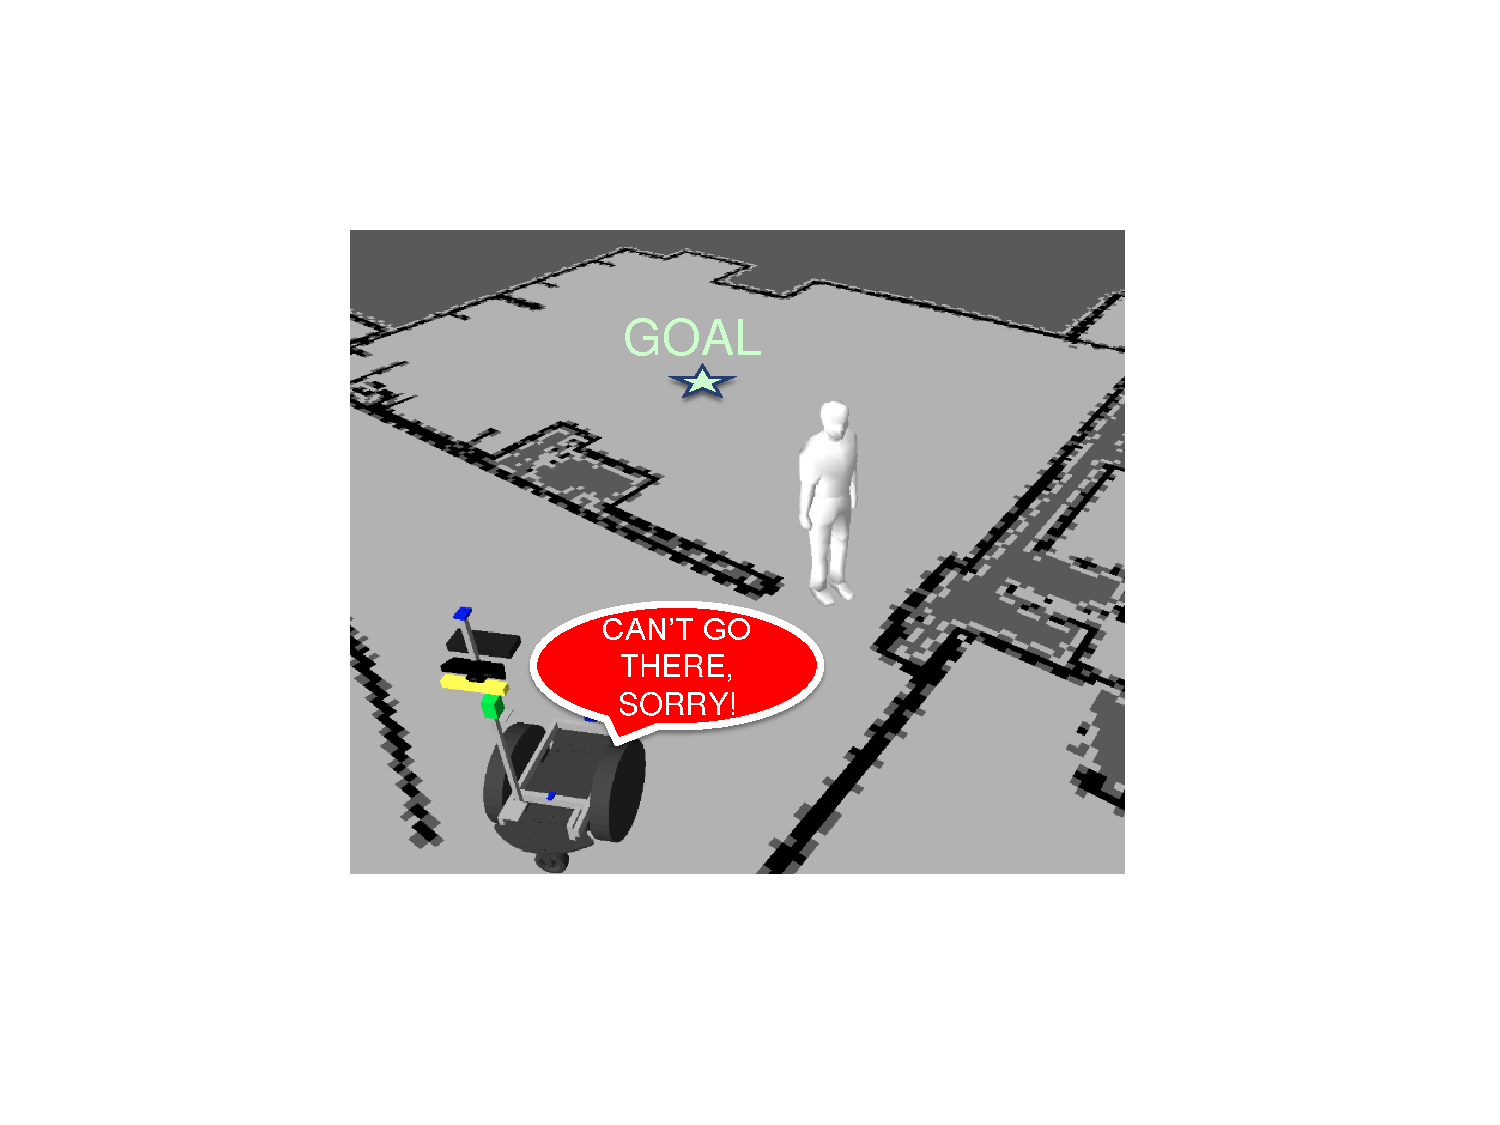
\includegraphics[width=0.5\textwidth]{pics/room_crop}
\caption{Standard path planners fail to produce a solution to the 'room problem'. Our people-aware planner anticipates that the human can give way to the robot if it approaches towards its goal.}
\label{fig:room}
\end{figure}

In this section, we propose a people-aware navigation planner that considers reactions of humans to robot motion. Our planner first first finds the least-cost map in the costmap that considers safety and disturbance of people. The costmap definition is discussed in Section \ref{sec:navigation_global_planner}. Then the path is refined by simulating people's reaction to robot's motion using Social Forces Model~\cite{helbing1995social}. The path refinement will be discussed in Section \ref{sec:navigation_path_refinement}. In dynamic simulation, robots and humans repulse each other, and additional forces helps to stay away from obstacles and conserve formation in groups. Paths are re-planned when the world state changes or humans does not move as anticipated. In Section \ref{sec:navigation_local_planner}, we discuss our local planner. We then discuss the implementation of the system in Section \ref{sec:navigation_results}, demonstrate two example scenarios in simulation in Section \ref{sec:navigation_results_simulation} and two on the real system in Section \ref{sec:navigation_results_real_robot}.


\subsection{Global Planner}
\label{sec:navigation_global_planner}

The global planner takes the start and goal positions and a 2D grid map as input and aims to find a set of waypoints that connects the start and goal cells. The output path has the minimum cost with regards to a cost function with 3 parameters: path length, safety and disturbance. We use A* search with Euclidean heuristics on a 8-connected grid map to find the minimum cost path. The configuration space obstacles are found by inflating the map obstacles for as much as the radius of the robot with the assumption that the robot is circular.

\textbf{Path length cost:}  Each action $a$ of the robot (moving to one of the 8 adjacent cells) has a non-negative action cost $Cost_{a}(x_{i},y_{i},a)$. If the destination cell is occupied by a configuration space obstacle, then the action cost is infinite. Otherwise, it is the distance in meters. The action cost is thus defined as:
\begin{align}
Cost_{a}(x_{i},y_{i},a)=\left\{ \begin{array}{cl}
u & \textrm{if $a$ = N, E, S, W}\\
u\sqrt{2} & \textrm{if $a$ = NW, NE, SW, SE}\\
\infty & \textrm{if  $Cell(x_{i+1}, y_{i+1})$ in obstacle} \end{array}\right.
\end{align}
where N,NW,.. are the grid cell expansion directions and $u$ is the grid cell size. The resulting path length cost of a path $P$ is then the sum of all action costs: 
\begin{align}
Cost_{path}(P) = \sum\limits_{a \in P} Cost_{a}(x_{i},y_{i},a)
\end{align}

\textbf{Safety cost:} The notion of safety is the absolute need of any human-robot interaction scenario. This cost is a human centered 2D Gaussian form of cost distribution and aims to keep a distance between the robot and the humans in the environment. While some approaches used un-isotropic cost functions to account for human orientation, we use a isotropic Gaussian for its simplicity. Each cell coordinate around a human contains a cost inversely proportional to the distance. Since the safety loses its importance when the robot is sufficiently far away from the human, safety cost becomes zero after a threshold distance. If there are multiple people in an environment, the safety cost of a cell takes its value from the closest human.
\begin{align}
Cost_{safety}(x,y)=\left\{ \begin{array}{cl}
u\max_{h\in H}(\mathcal{N}(\mu_h,\sum)) & \textrm{if $d<d_{max}$}\\
0 & \textrm{if $d\geq d_{max}$}\\
\end{array}\right.
\end{align}

where d is the distance to the closest human, H is all humans, $\mu_h = (|x - h.x|,|y - h.y|)$ and $\sum = 0.5I_2$ is a fixed covariance matrix. The multiplication by the grid cell size compensates for the grid map resolution. Otherwise, for example, if a very fine map was used, safety cost would dominate the path length and disturbance costs, which are independent of the map resolution.
 
\textbf{Disturbance cost:} This cost is aimed to represent the cases where the robot potentially disturbs the interaction of a group of humans. For example, if two people are facing each other and talking, then the robot should not cross between them.  We model this with a disturbance cost that is introduced if a path crosses between two people. We do not detect if there actually is conversation between the people, but estimate the disturbance cost using body poses of agents. This cost increases if body orientations of two people are facing each other and is inversely proportional on the distance between the two humans.

For each step taken in the grid, we check if the line segment from the current position to the  projected position intersects a line segment between all pairs of humans. To illustrate, let's assume the robot crosses the line between human A and human B in Figure~\ref{fig:disturbance}. 

The disturbance cost is calculated as:
\begin{align} 
\begin{split} 
Cost_{dist}(x,y,a)&=\max(0, f(d).(\vec{AA'}.\vec{AB}+\vec{BB'}.\vec{BA})) \\
f(d)&=\frac{1}{d}-\frac{1}{d_{max}}
\end{split} 
\end{align}

where all the vectors are normalized and $d_{max}$ is the maximum distance between the humans that returns a disturbance cost. Figure~\ref{fig:disturbance_ex} illustrates several examples of disturbance costs with $d_{max}=3$ meters.

\begin{figure}[ht!]
\centering
%
        \subfigure[]{%
            \label{fig:disturbance}
            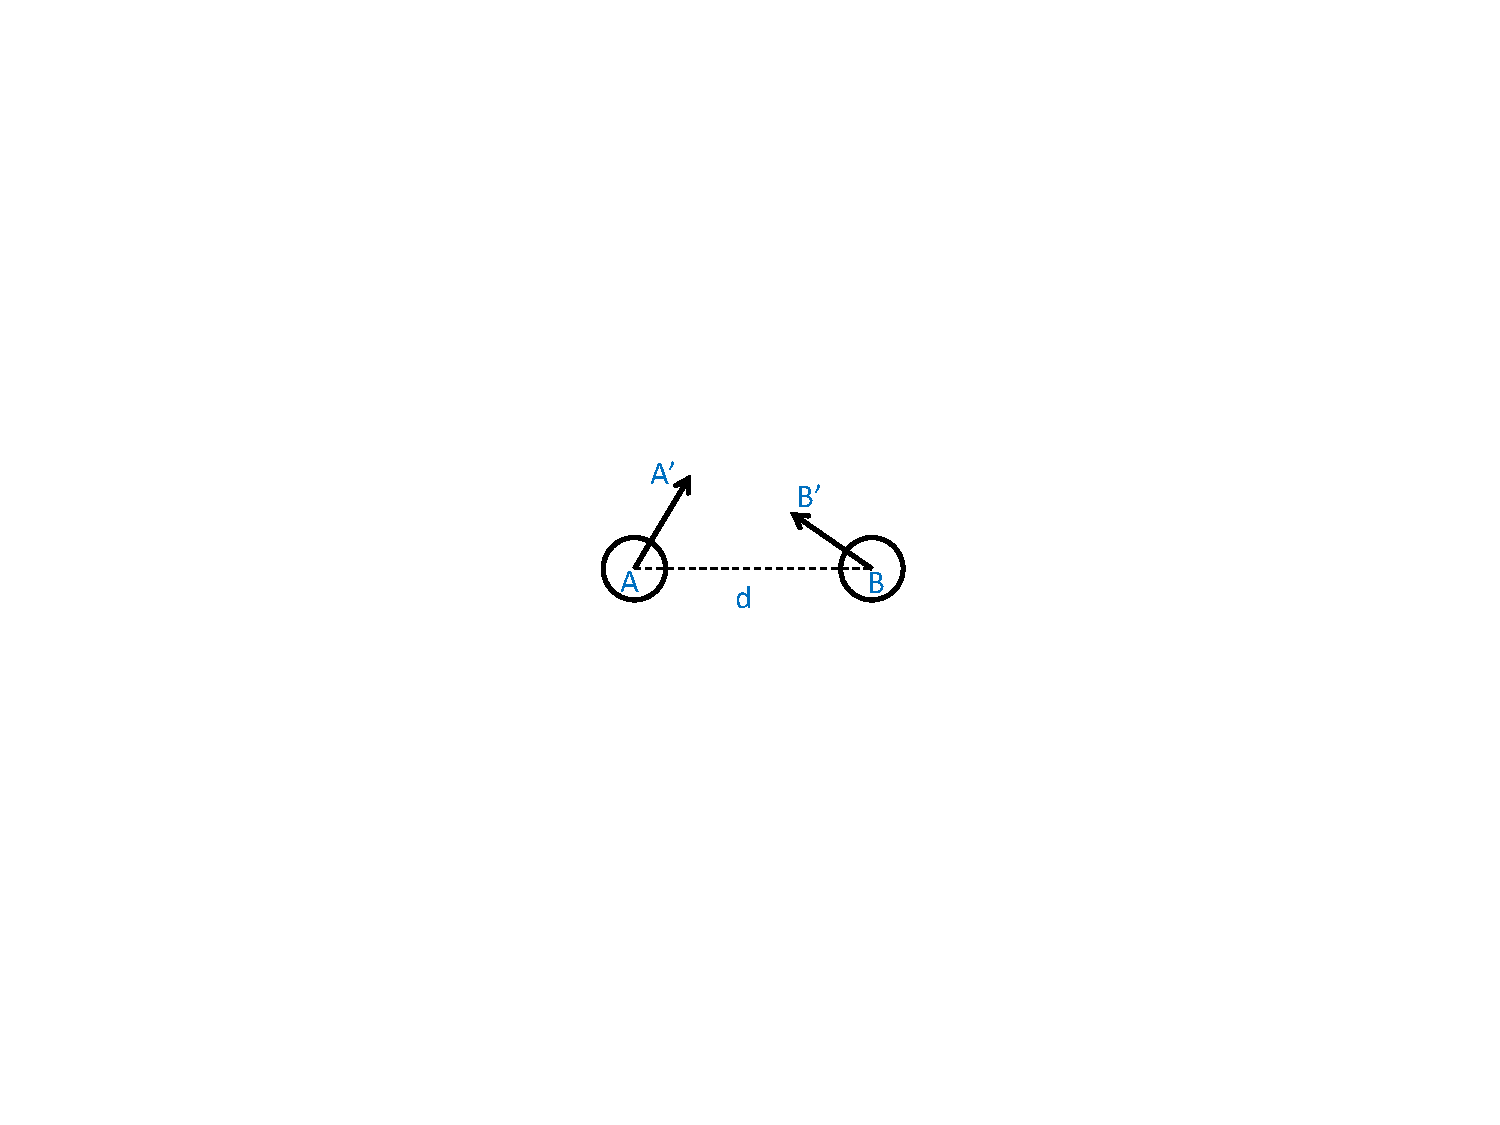
\includegraphics[width=0.32\textwidth]{pics/disturbance_crop}
        }%
        \subfigure[]{%
           \label{fig:disturbance_ex}
           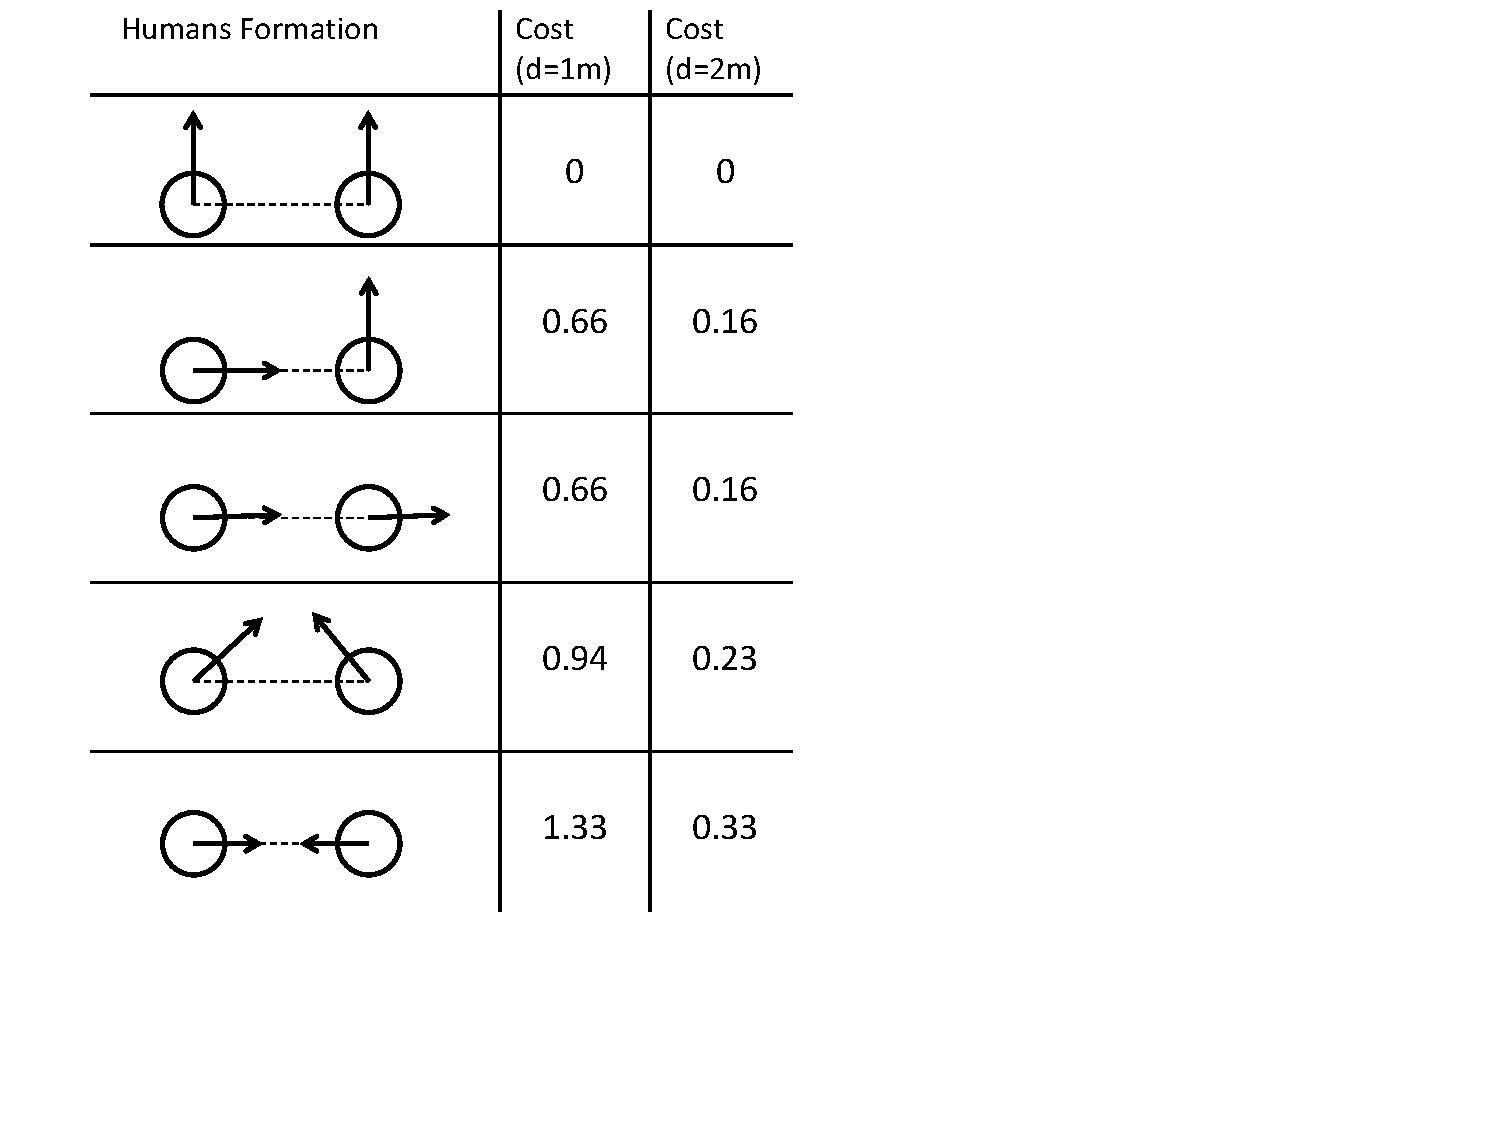
\includegraphics[width=0.4\textwidth]{pics/disturbance_ex_crop}
        }        
    \caption{%
	Disturbance costs in different human-human configurations and distances. A path that crosses the dashed lines incurs the disturbance cost calculated on the right side.
     }%
   \label{fig:sim}
   \vspace{-0.2cm}
\end{figure}



\textbf{Total Cost:} The total cost of a path $P$ is computed with a weighted average of path length, safety and disturbance costs. We use A* search to find the least-cost path.
\begin{align}
Cost_{Total}(P) = Cost_{path}+w_{s}.Cost_{safety} + w_d.Cost_{dist}
\end{align}

\subsubsection{Path Refinement using Social Forces}
\label{sec:navigation_path_refinement}

In this section, we describe the path refinement process that is applied to the global path. The initial geometric path generated by the global planner is not smooth, therefore robot motion might not be easy to interpret for human observers. The path refinement processes the global plan and simulates the parts of the path where group of humans are closeby. We use Social Forces Model (SFM) \cite{helbing1995social} to simulate the motions of both humans and the robot. Interaction between people are modeled as attractive and repulsive forces in SFM, similar to the Potential Field Method \cite{khatib1986real} for robot navigation. The forces are recomputed iteratively and the resulting simulated paths replaces the corresponding path sections in the global plan.

First, groups of people are found by clustering with respect to their positions. Simple euclidean distance thresholding is used for clustering. In our current implementation, a group region is defined as a rectangle, although other shapes are also possible. The path refinement process receives the global plan and finds out where it enters and exits each group region if it intersects the region. Goal of the dynamic iterative simulation is to find a sub-plan between those two points. Forces apply to all agents, including the robot and humans. We define 4 forces acting on the agents:
\begin{itemize}
  \item $F_{goal}$ : attraction towards a sub-goal
  \item $F_{social}$ : repulsion from other agents
  \item $F_{obs}$ : repulsion from nearest obstacle
  \item $F_{group}$ : attraction or repulsion towards group members
\end{itemize}
The forces acting on the robot at the first iteration of forces simulation are illustrated on the robot in Figure~\ref{fig:forces_robot}. The force magnitudes with respect to distances between entities are plotted in Figure \ref{fig:socialforces}. 

\begin{figure}[ht!]
\centering
%
        \subfigure[]{%
            \label{fig:forces_robot}
            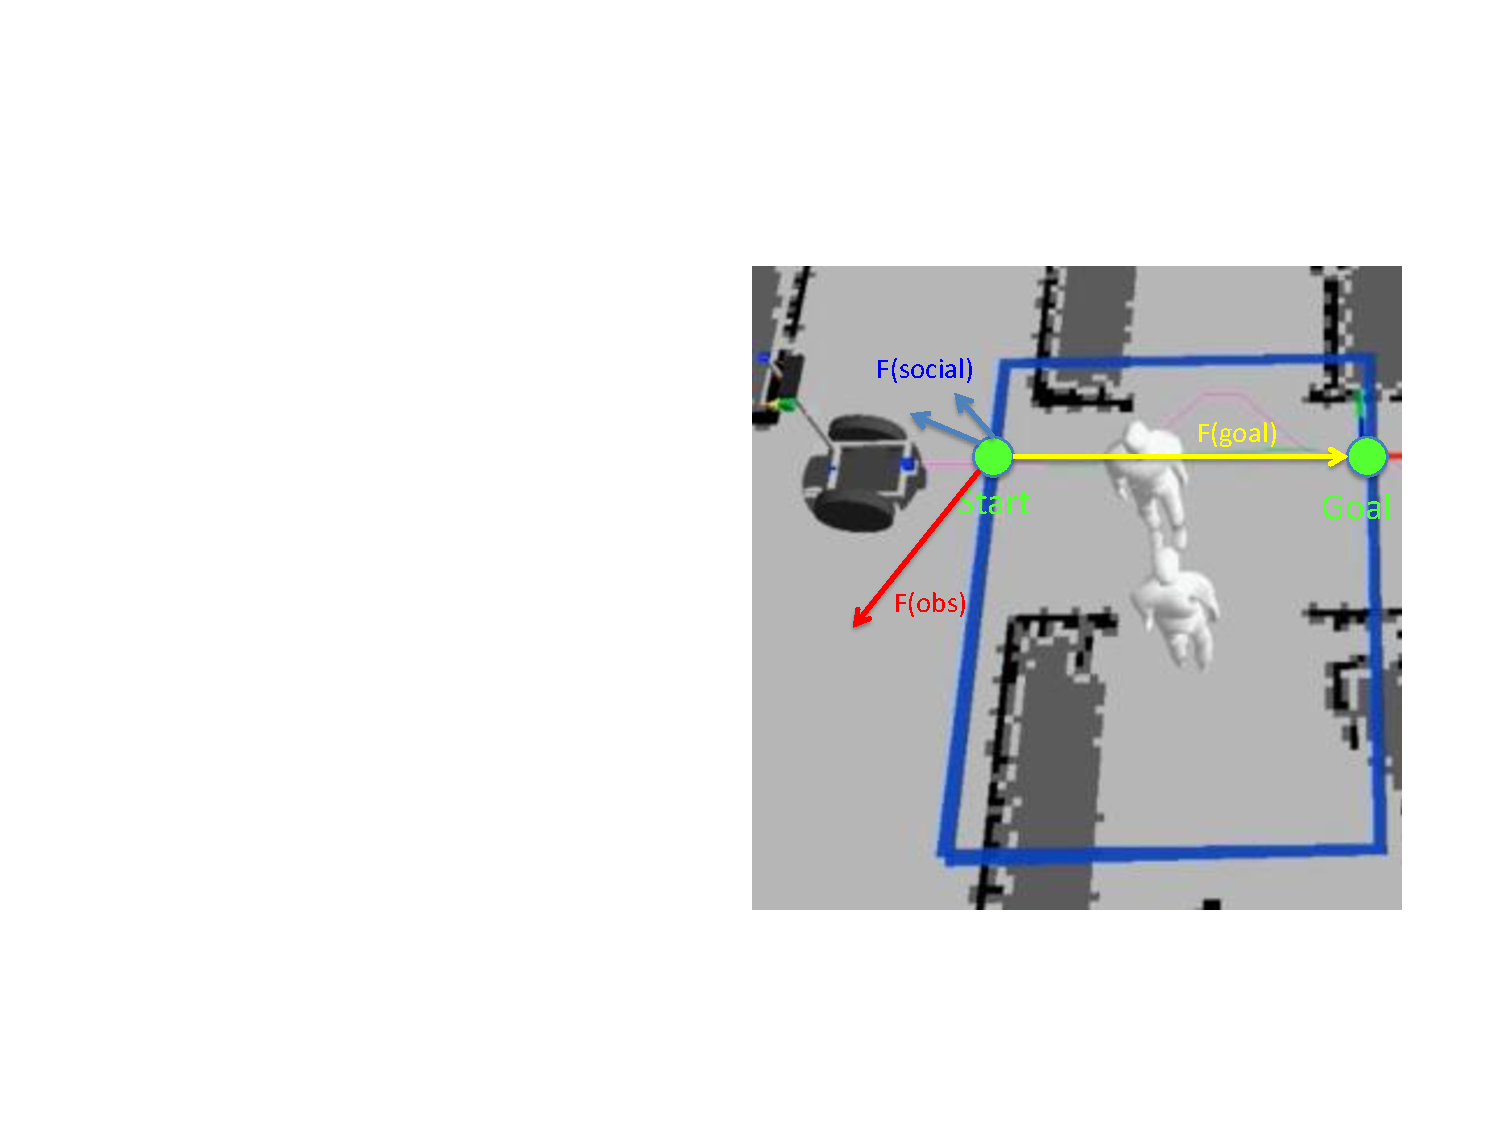
\includegraphics[width=0.43\textwidth]{pics/forces_robot_crop}
        }%
        \subfigure[]{%
           \label{fig:socialforces}
           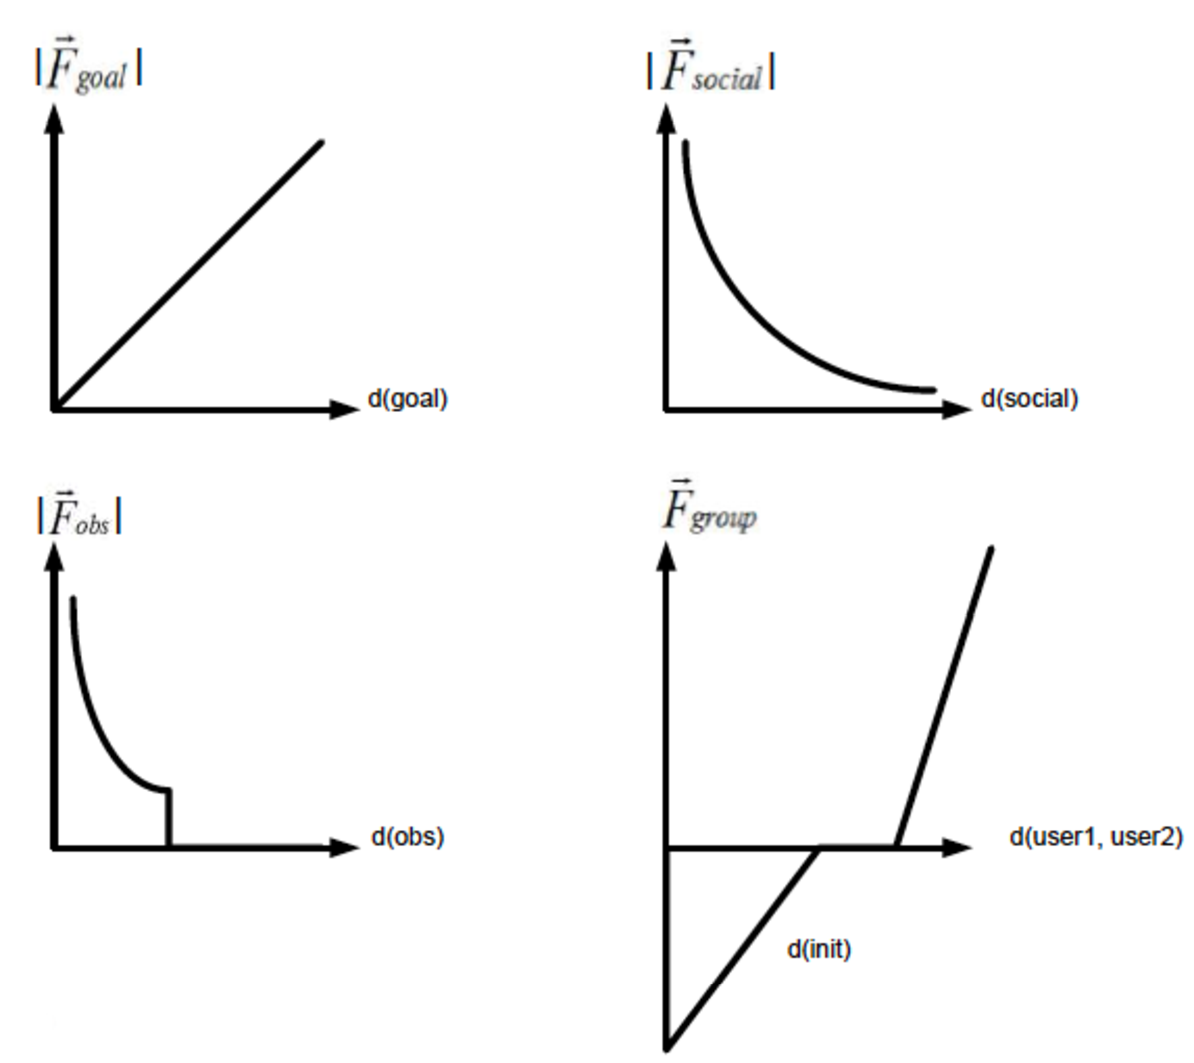
\includegraphics[width=0.53\textwidth]{pics/socialforces}
        }        
    \caption{%
	a) Social forces acting on the robot, including $F_{goal}$,$F_{social}$,$F_{obs}$, are shown at the first iteration of the dynamic planner. Note that $F_{group}=0$ as the robot does not belong to a group. The group force (not shown) exists, however, for the humans as they are in the same group region. b) Social forces with respect to the distance towards the corresponding entity.
     }%
   \label{fig:forces}
\end{figure}


Starting from the first group region that intersects the static plan, the following procedure is applied within every group region: At every iteration, first the resultant force vector acting on the robot is found. Then the planner takes a step in the direction of the $F$ vector for a fixed step size. Then each of the humans in the group takes a step towards the resultant force that is acting on them. The planner continues the iterations until a solution is found. If a solution is found, the calculated sub-plan replaces the static plan in this group region. Potential fields are known to stuck to local minima~\cite{koren1991potential}, and the planner might go into infinite loop. We stop the planner after a number of iterations and accept the static plan in the corresponding group region if that happens.

We assume that humans have a cognitive model of the robot, by thinking that the robot has a limited Field of View (FOV). When the robot has gone past a human (out of the FOV), then we make the repulsion force $F_{social}=0$. We think that humans behave that way: as someone walks past, there are no social constraints resulting from that individual any more.

\subsection{Local Planner}
\label{sec:navigation_local_planner}

The local planner is responsible for finding the trajectory that the robot is capable of executing. It accepts a geometric global path as input and computes the linear and angular velocity necessary to follow the dynamic path. We adopt a local planner inspired by Dynamic Window Approach (DWA) by Fox \cite{fox1997dynamic}. In the original DWA approach, only circular trajectories are considered, defined by pairs $(v,w)$ of linear and angular velocities. An objective function, consisting of target heading, clearance from obstacles and velocity of the robot is maximized by sampling admissible velocities.

Our approach also samples admissible velocities, but the optimization criteria we use consists only of the Euclidean distance to a sub-goal point chosen on the path that is ahead of the robot. The velocity pair that resulted in the closest proximity to the sub-goal is chosen and sent to robot controllers. At every control iteration, the sub-goal is chosen as the first point ahead of the robot that is further than a distance threshold. We found that a threshold of 0.25 meters was sufficient to choose the sub-goal. After the local planner calculates the output velocities, they are applied to the robot and the iterative process continues until the the robot reaches the goal. Since the goal is a singular point, it is impossible for the robot to be exactly at the goal. Therefore, a tolerance around the goal point, defined as a circle around the goal is defined.

Given the robot's current pose and an applied velocity, the DWA approach requires to have a motion model for the robot. The motion model projects the what the robot pose would be, if a velocity pair is applied to it for a time period. The robot we used for our implementation is a non-holonomic two wheeled robot. While one can use the general motion equations derived in \cite{fox1997dynamic}, we used linear approximated motion equations for our robot in Equation \ref{eq:motion_model}. Given a robot pose $q^t=(x^t,y^t,\theta^t)$ at time $t$ and an input velocity $(v,w)$, the projected robot pose at time $t+\Delta t$ is:

\begin{align}
q^{t+\Delta t} = 
f_{motion}(q^t,v,w,\Delta t) =
\begin{Bmatrix}
x^t-\frac{v}{w}sin(\theta^t)+\frac{v}{w}sin(\theta^t+w \Delta t)\\
y^t+\frac{v}{w}cos(\theta^t)-\frac{v}{w}cos(\theta^t+w \Delta t)\\
\theta^t + w\Delta t
\end{Bmatrix}
\label{eq:motion_model}
\end{align}


%We use  for obstacle avoidance of non-holonomic robots. (TODO: DWA our version, derive motion model, vs. ) DWA samples linear and angular robot velocities and simulates the robot trajectory for each of them. First, a waypoint on the dynamic path is chosen as a sub-goal. At every control iteration, the waypoint is chosen as the first point ahead of the robot that is further than a distance threshold. We found that a threshold of 0.25 meters was sufficient. Robot is simulated with each velocity combination and the trajectory that gets closest to the sub-goal is sent to the motor controllers.

\subsection{Results}
\label{sec:navigation_results}

In this section, we provide qualitative results both in simulation and on the real robot. We used a non-holonomic drive robotic platform, Segway RMP-200, for the real experiments. We used our laser-based torso tracking method presented in Section \ref{sec:multimodal_torso_detection}.

\subsubsection{Simulation}
\label{sec:navigation_results_simulation}

\begin{figure}[h!]
\centering
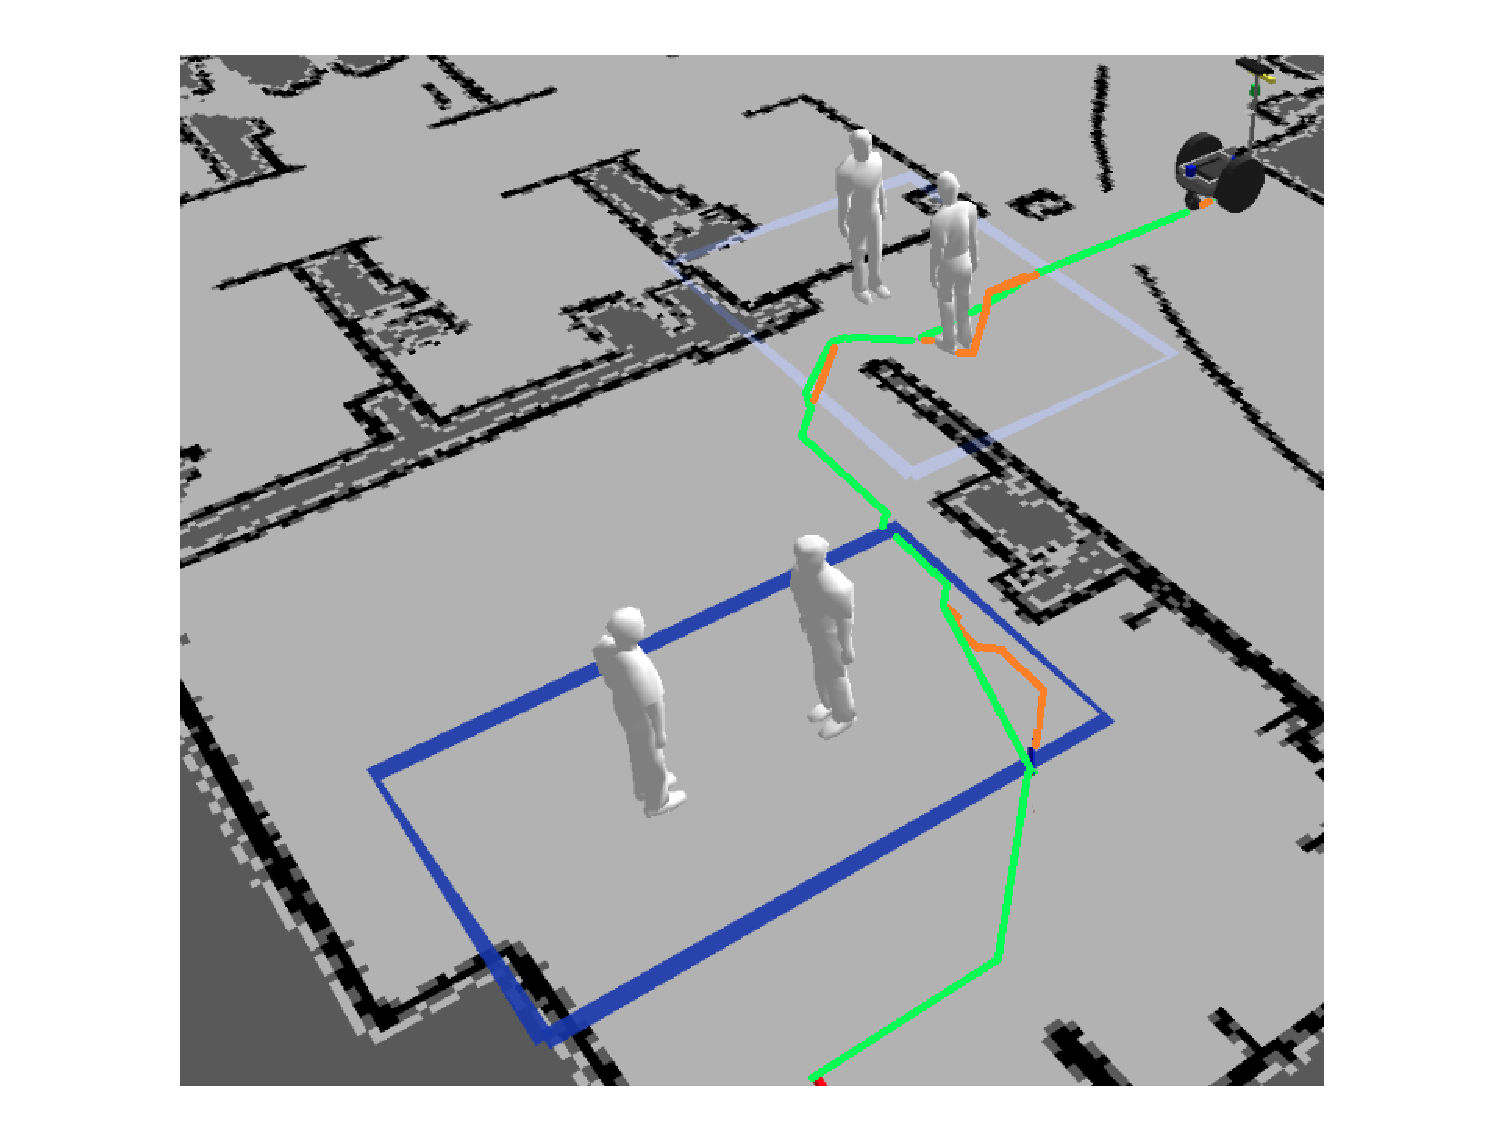
\includegraphics[width=0.5\textwidth]{pics/room_sol_crop}
\caption{"Room Problem". The robot is outside a room and the goal is inside the room. Traditional planners can not solve the problem because two people are blocking the doorway. Our planner generates a tentative path, with the initial global plan shown in green and the dynamic refinements are shown in orange.}
\label{fig:room_sol}
\end{figure}

\begin{figure}[hbtp]
\centering
        \subfigure[]{%
            \label{fig:sim2}
            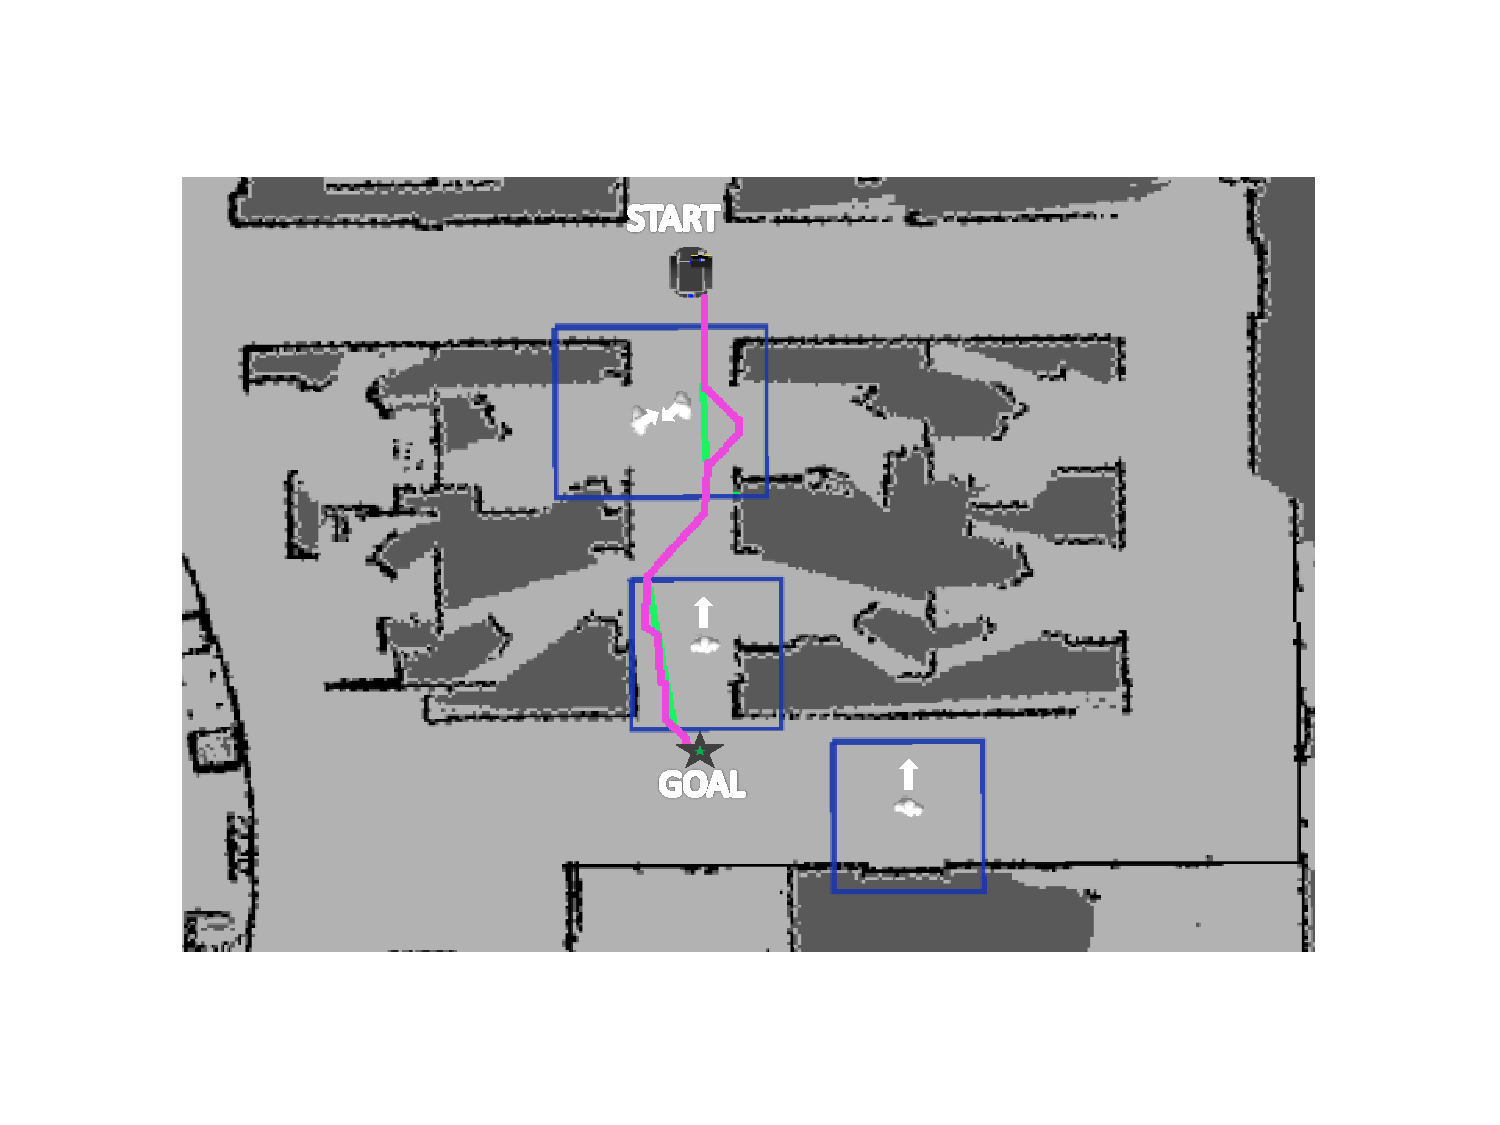
\includegraphics[width=0.6\columnwidth]{pics/sim2_crop}
        } \\
        \subfigure[]{%
           \label{fig:sim3}
           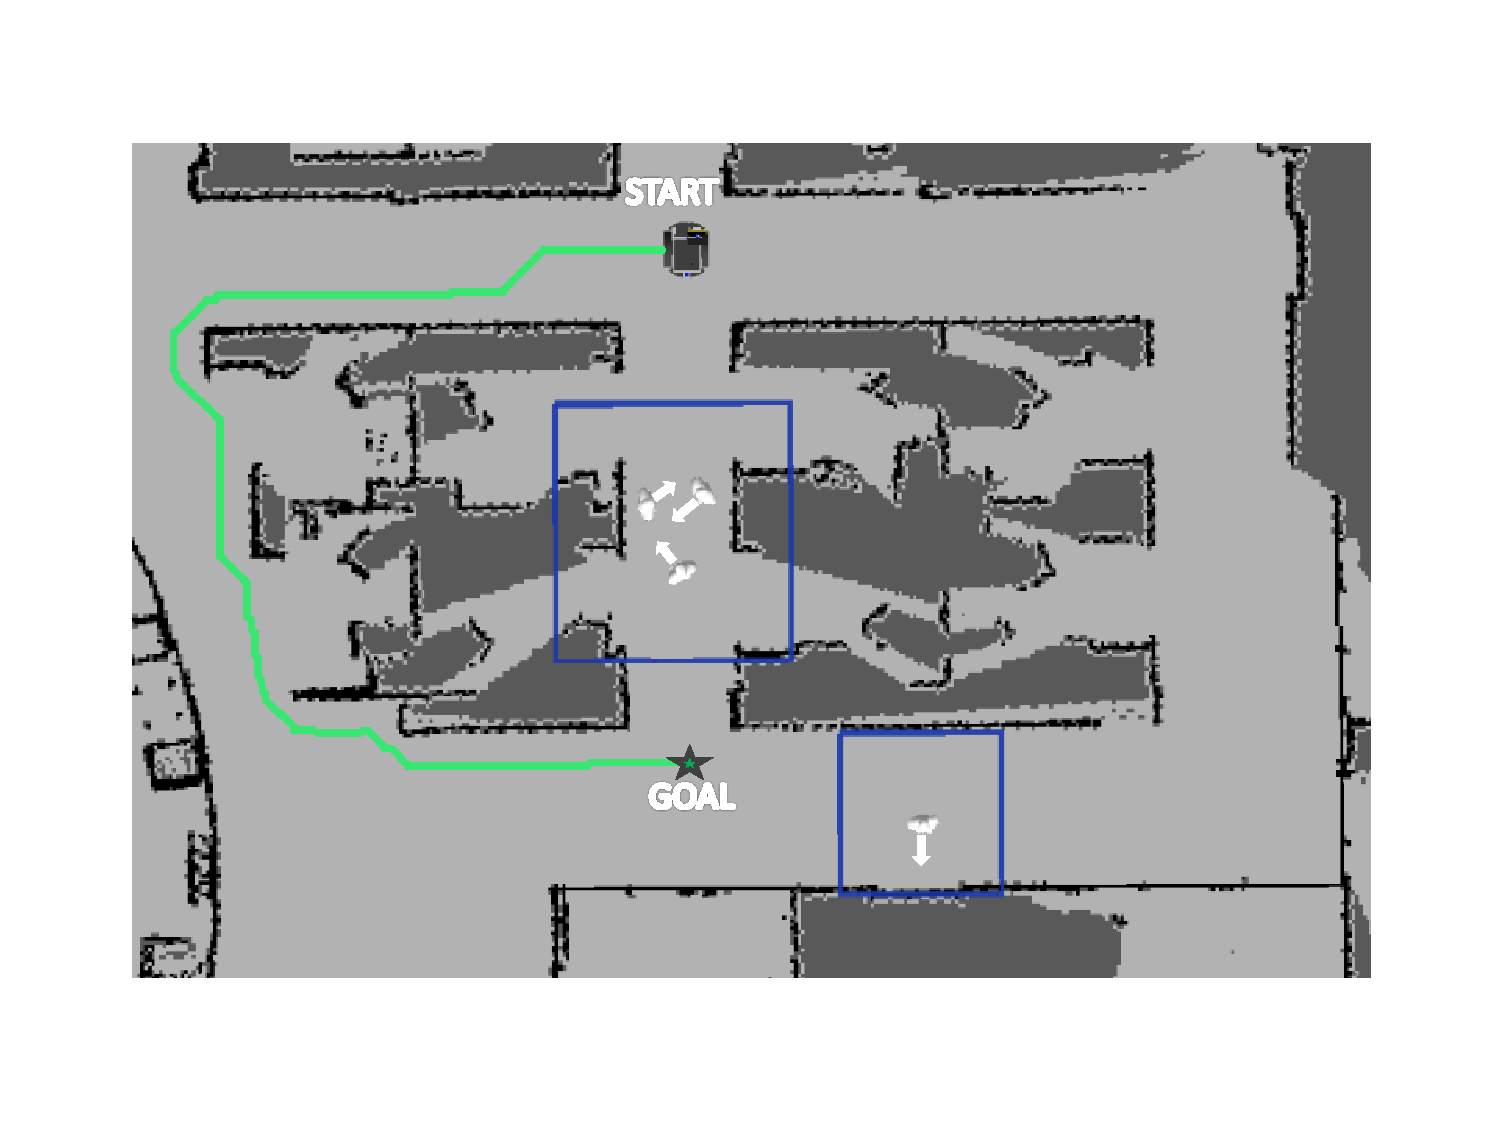
\includegraphics[width=0.6\columnwidth]{pics/sim3_crop}
        }
	\subfigure[]{%
           \label{fig:sim1}
           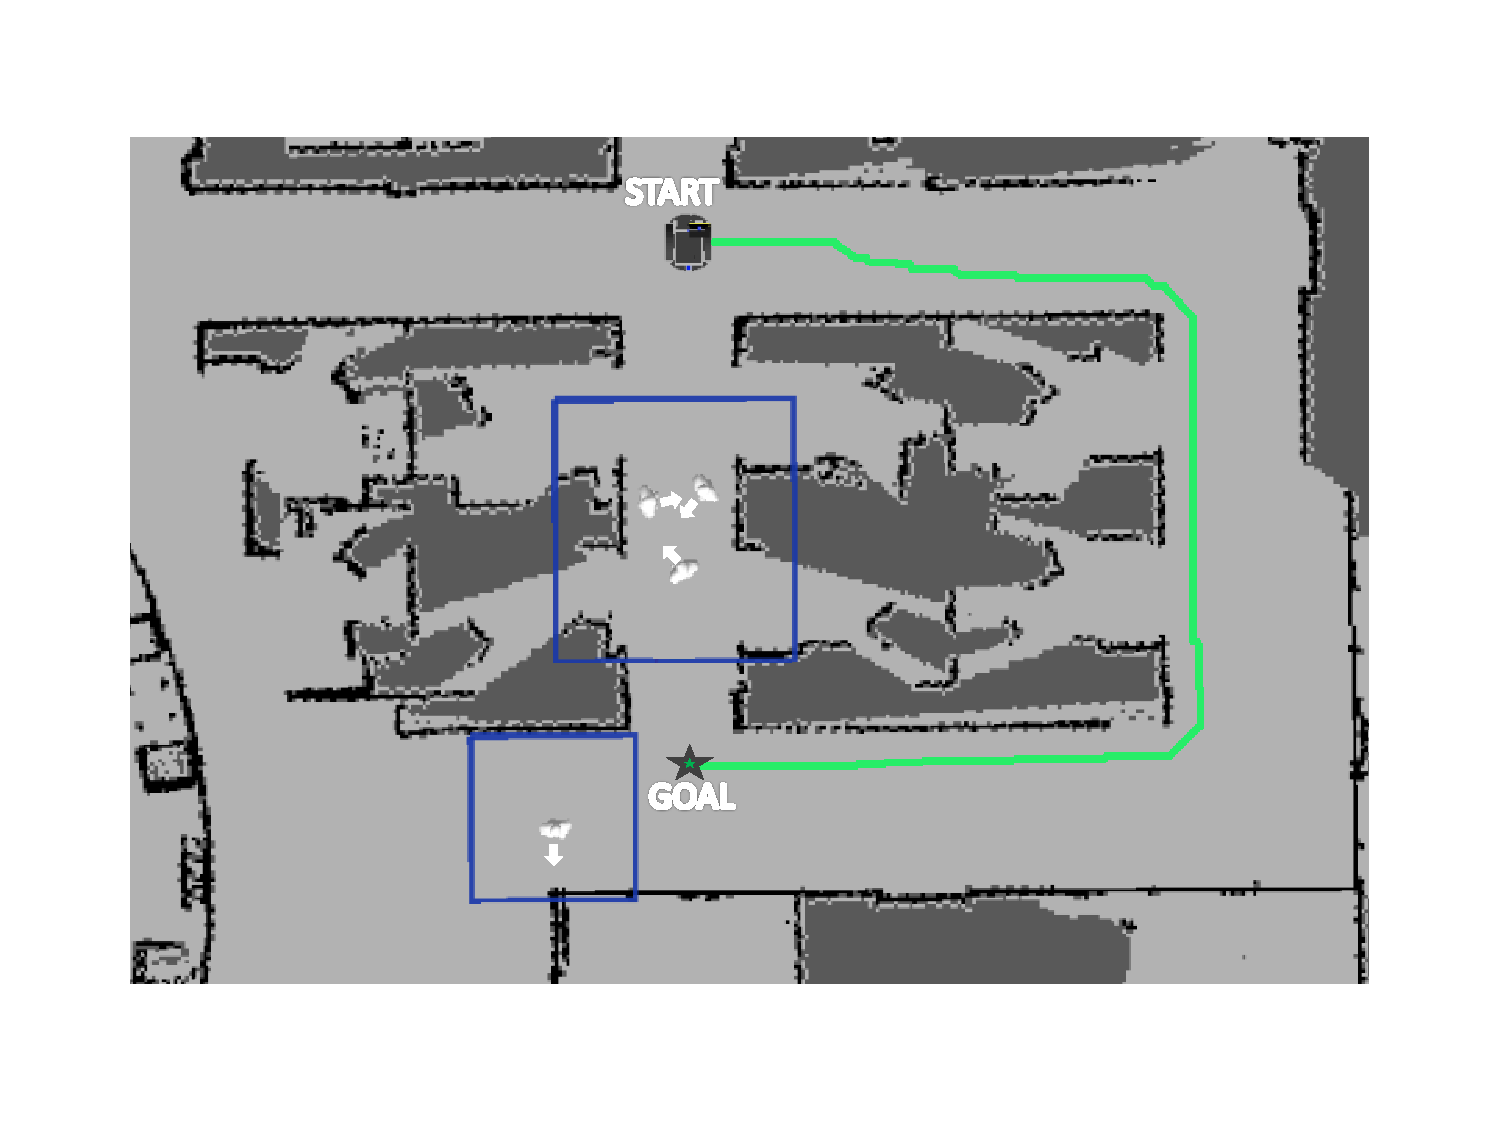
\includegraphics[width=0.6\columnwidth]{pics/sim1_crop}
        }        
    \caption{%
	Paths differ drastically with the poses and grouping of humans. a) The robot takes shortest route, traveling in the vicinity of a group of two and another individual. b) third individual joins the group. Robot takes a longer path that doesn't have humans on path. c) fourth person changes his position, leading the robot to take the longest route.
     }%
   \label{fig:sim}
\end{figure}


\textbf{Room Problem: } In this scenario, the robot is outside the room and a point inside the room is given as the goal (Figure~\ref{fig:room_sol}). Traditional planners can not return a solution in this scenario because there is not enough space for the robot to navigate inside. There are two people standing at the doorway and there are two more standing people inside. The static plan and dynamic plans are shown in green and orange, respectively. This path is planned for the current time but makes assumptions about future positions of humans. Note that the dynamic planner modifies only the parts of plan inside group regions (blue rectangles). In the first group region (doorway), the static plan involves going between the humans. Dynamic simulation suggests that people will get closer to each other if the robot drives towards the side. In the second group region, since two humans are oriented to each other, going between them would add a high disturbance cost, therefore the static plan avoids going between them. Safety costs encourages staying far from the humans, but not too far because a longer path would increase the path length cost. The robot is further led to stay closer to the room boundaries in the dynamic planner due to the repulsive forces from both humans.




\textbf{Office Environment: } Goal of the robot is to navigate to a goal position in an office environment with 4 standing people (Figure~\ref{fig:sim}). In this scenario, we show how the planned path is drastically changing with the poses of humans even though the start and goal position of the robot doesn't change. There are 3 main ways the robot can navigate to its goal: left, center or right corridor. 

In the first configuration in Figure~\ref{fig:sim2}, two people are grouped together as they are looking at each other and likely conversing. The robot decides to take the center corridor, first slightly disturbing the speaking duo, then switches sides in the corridor and reaches its goal. In the figure, the dynamic path (pink line) is overlaid on the static path (green line). 

In the second configuration in Figure~\ref{fig:sim3}, The third person at the center corridor joins the conversation. Now we have 2 group regions (rectangles) in the scene. Since passing through a group of 3 people would introduce a high disturbance cost in addition to the safety cost, the robot decides to take a longer route (left corridor). Since this path does not intersect any group regions, no dynamic simulation is done.

In the third configuration in Figure~\ref{fig:sim1}, the group of three hasn't moved, but the fourth person person has changed its position. In this case, if the left corridor is taken again, an additional safety cost would be incurred. Therefore the robot decides to take the longest route (right corridor). Again, since the robot travels far from humans, no dynamic simulation is done.

\subsubsection{Real Robot}
\label{sec:navigation_results_real_robot}


We demonstrate our anticipatory navigation planner on the real system in two environments: hallway and kitchen. Each scenario is run twice under different human positions and behaviors in order to show how the planner responds.

\textbf{Hallway passing: } In this scenario (Figure~\ref{fig:corridor}), robot's goal is to navigate to the end of the hallway. In the first run, humans move as the robot anticipates. In the second run, humans do not move as anticipated, and the robot adjusts its path. Each step is described in the caption of the figure. In both cases, the initial plan is to disturb the interaction by going between the two. This is because the safety cost for getting close to one of the humans was more dominant than the disturbance cost.

\textbf{Narrow corridor:} In this scenario (Figure~\ref{fig:kitchen}), robot's goal is to drive towards the exit door. There are 3 people nearby the robot. The robot can either take the shorter route that is the direct path, or take a longer path that is to the left of the table. Each important step is described in the caption of the figure. The first run shows that the robot may plan hoping to influence the human. The second run shows that the robot may take a longer route if the disturbance and safety costs are going to be large.

\begin{figure}[p!]
\centering
%
        \subfigure[]{%
            \label{fig:corridor1}
            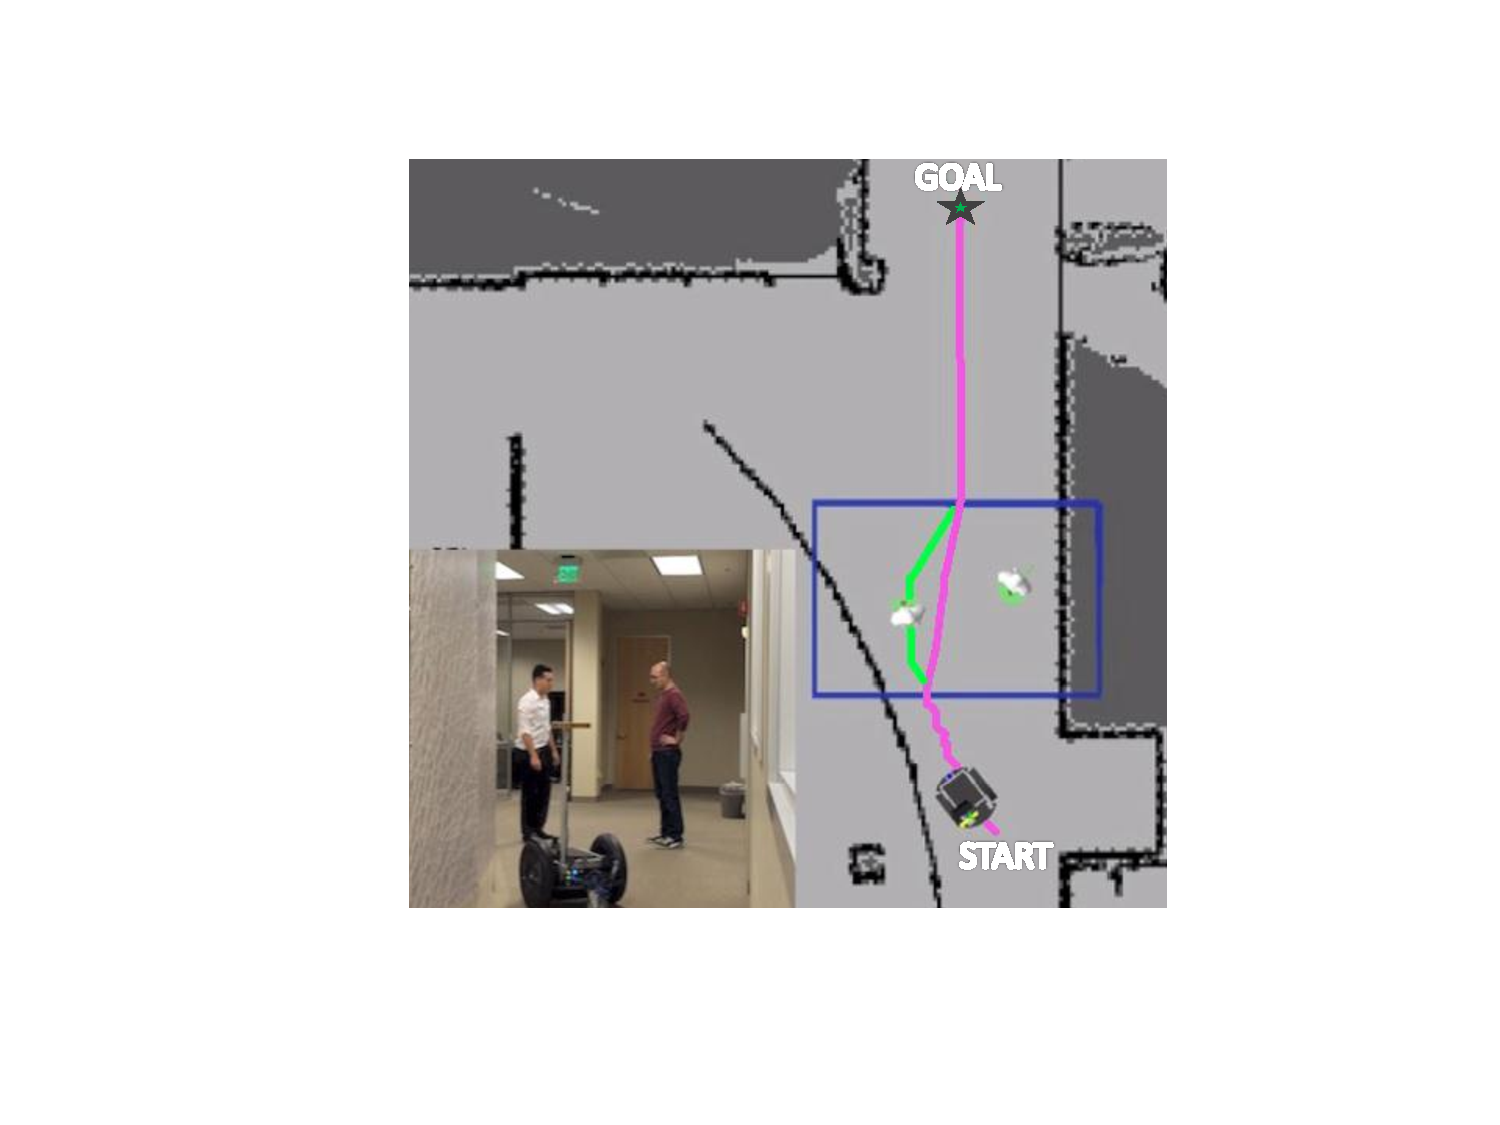
\includegraphics[width=0.58\columnwidth/2]{pics/corridor1_crop}
        }%
        \subfigure[]{%
           \label{fig:corridor2}
           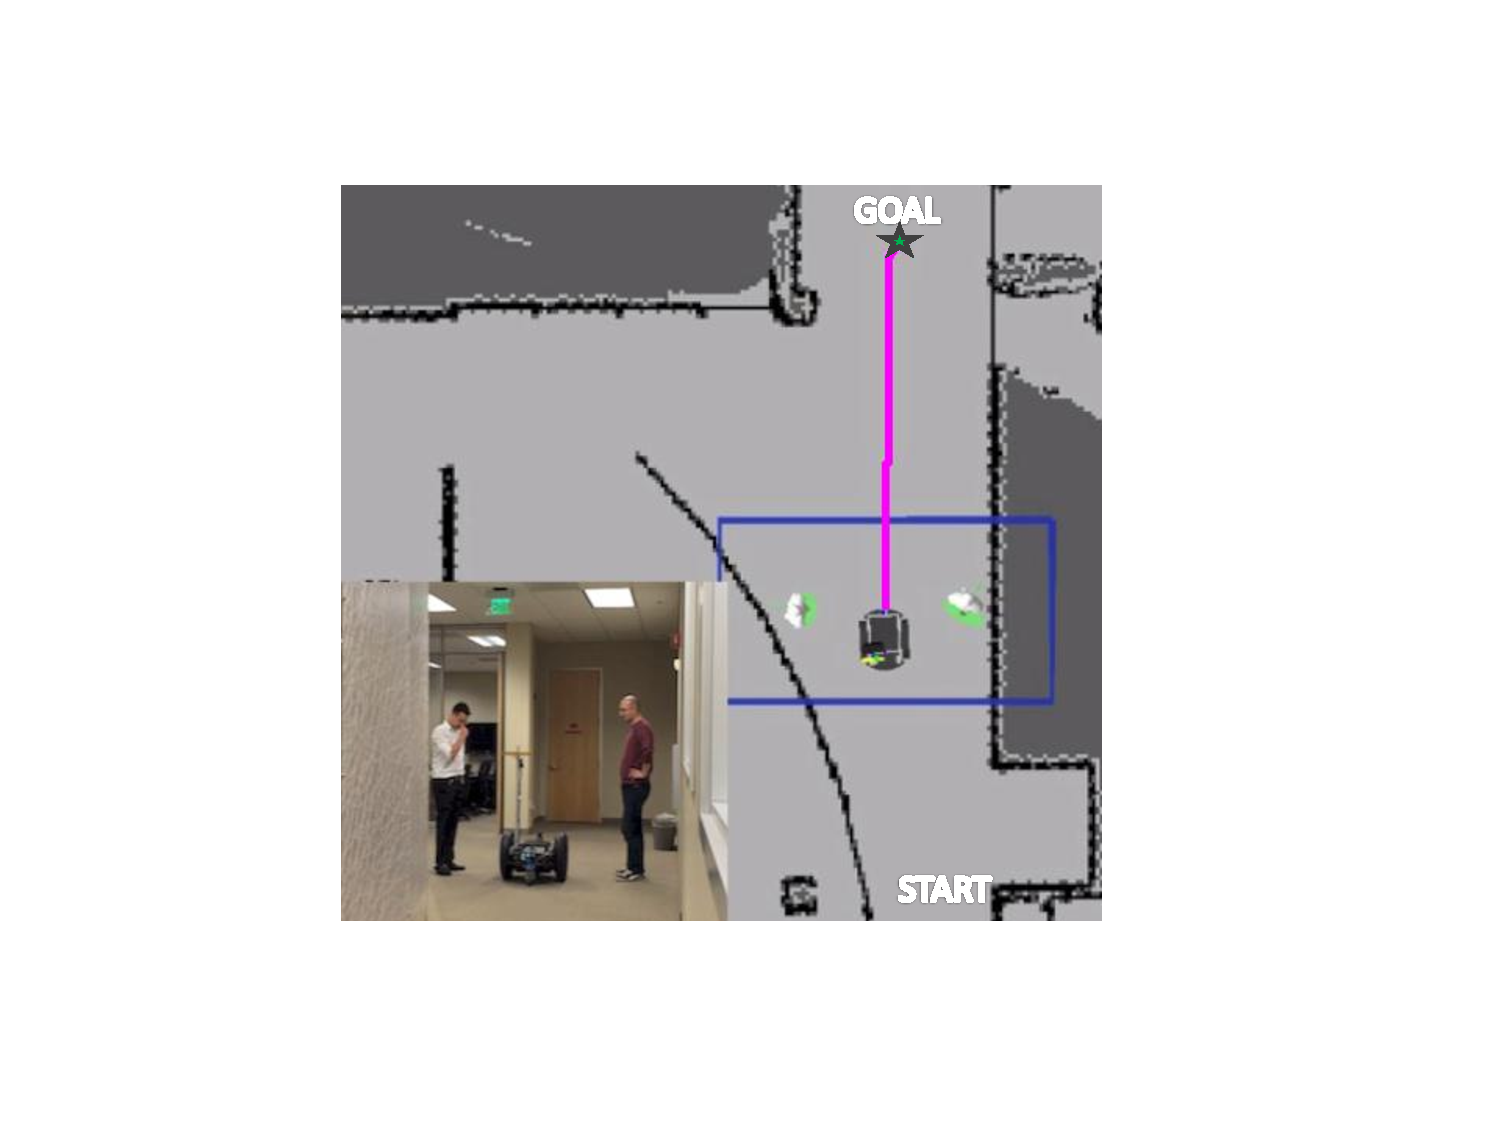
\includegraphics[width=0.58\columnwidth/2]{pics/corridor2_crop}
        }
        \subfigure[]{%
           \label{fig:corridor3}
           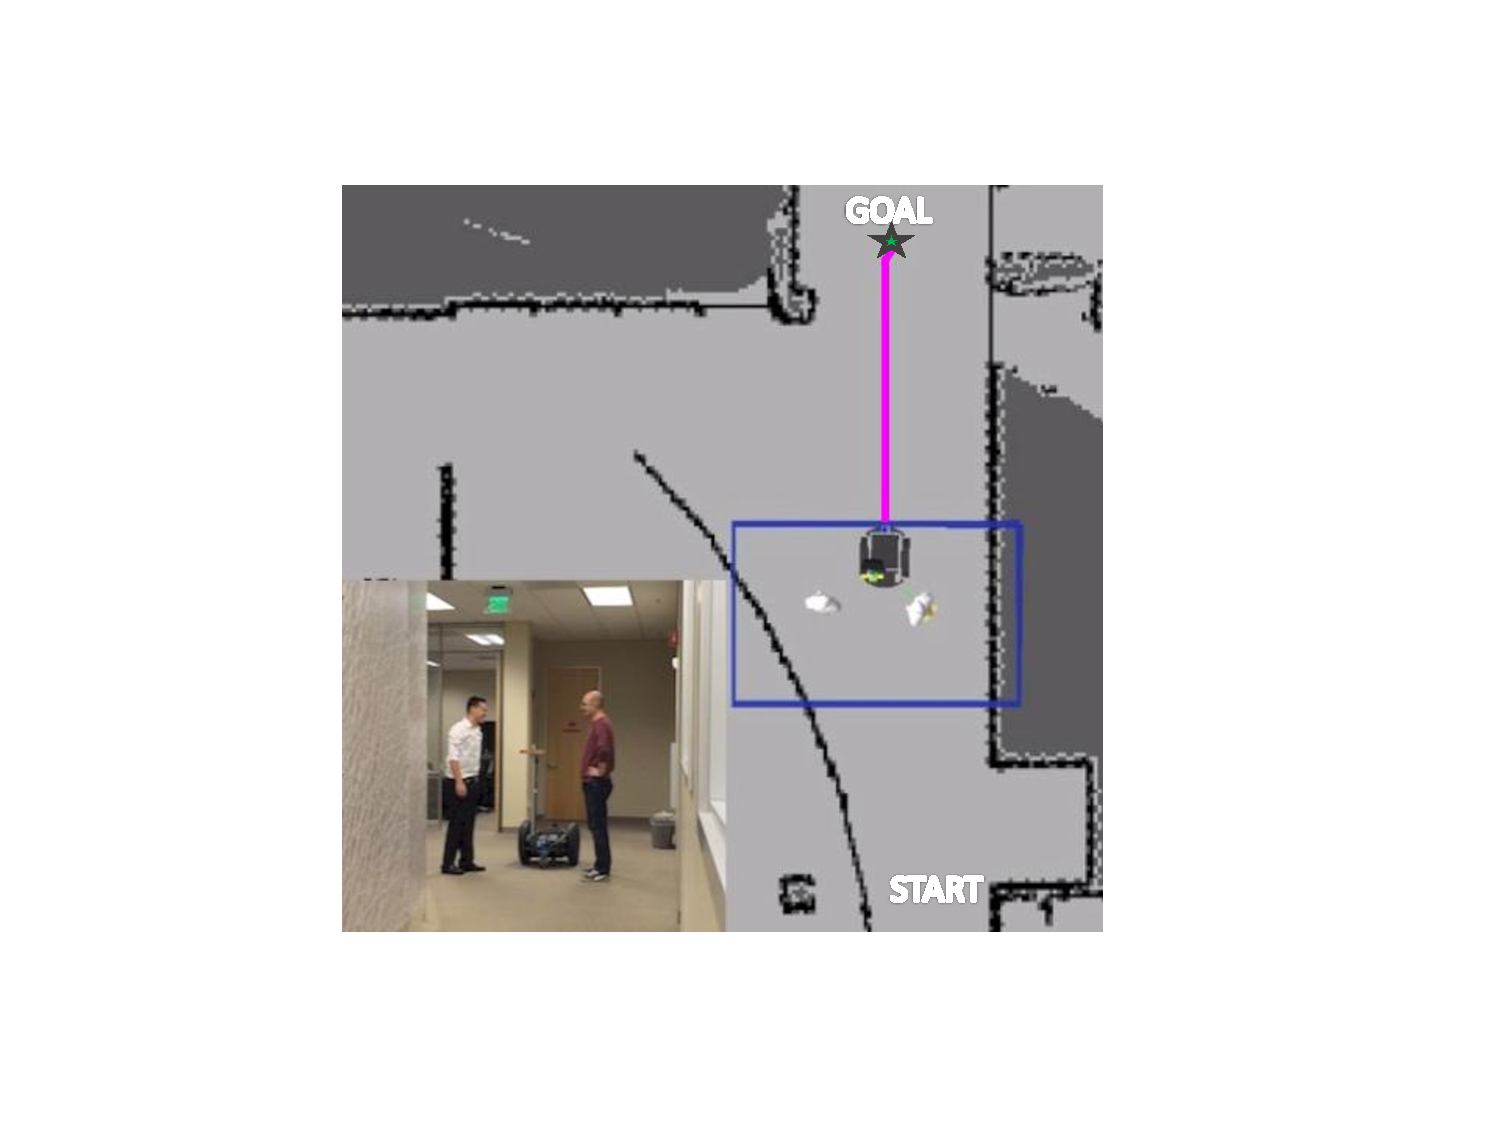
\includegraphics[width=0.58\columnwidth/2]{pics/corridor3_crop}
        }
\subfigure[]{%
           \label{fig:corridor4}
           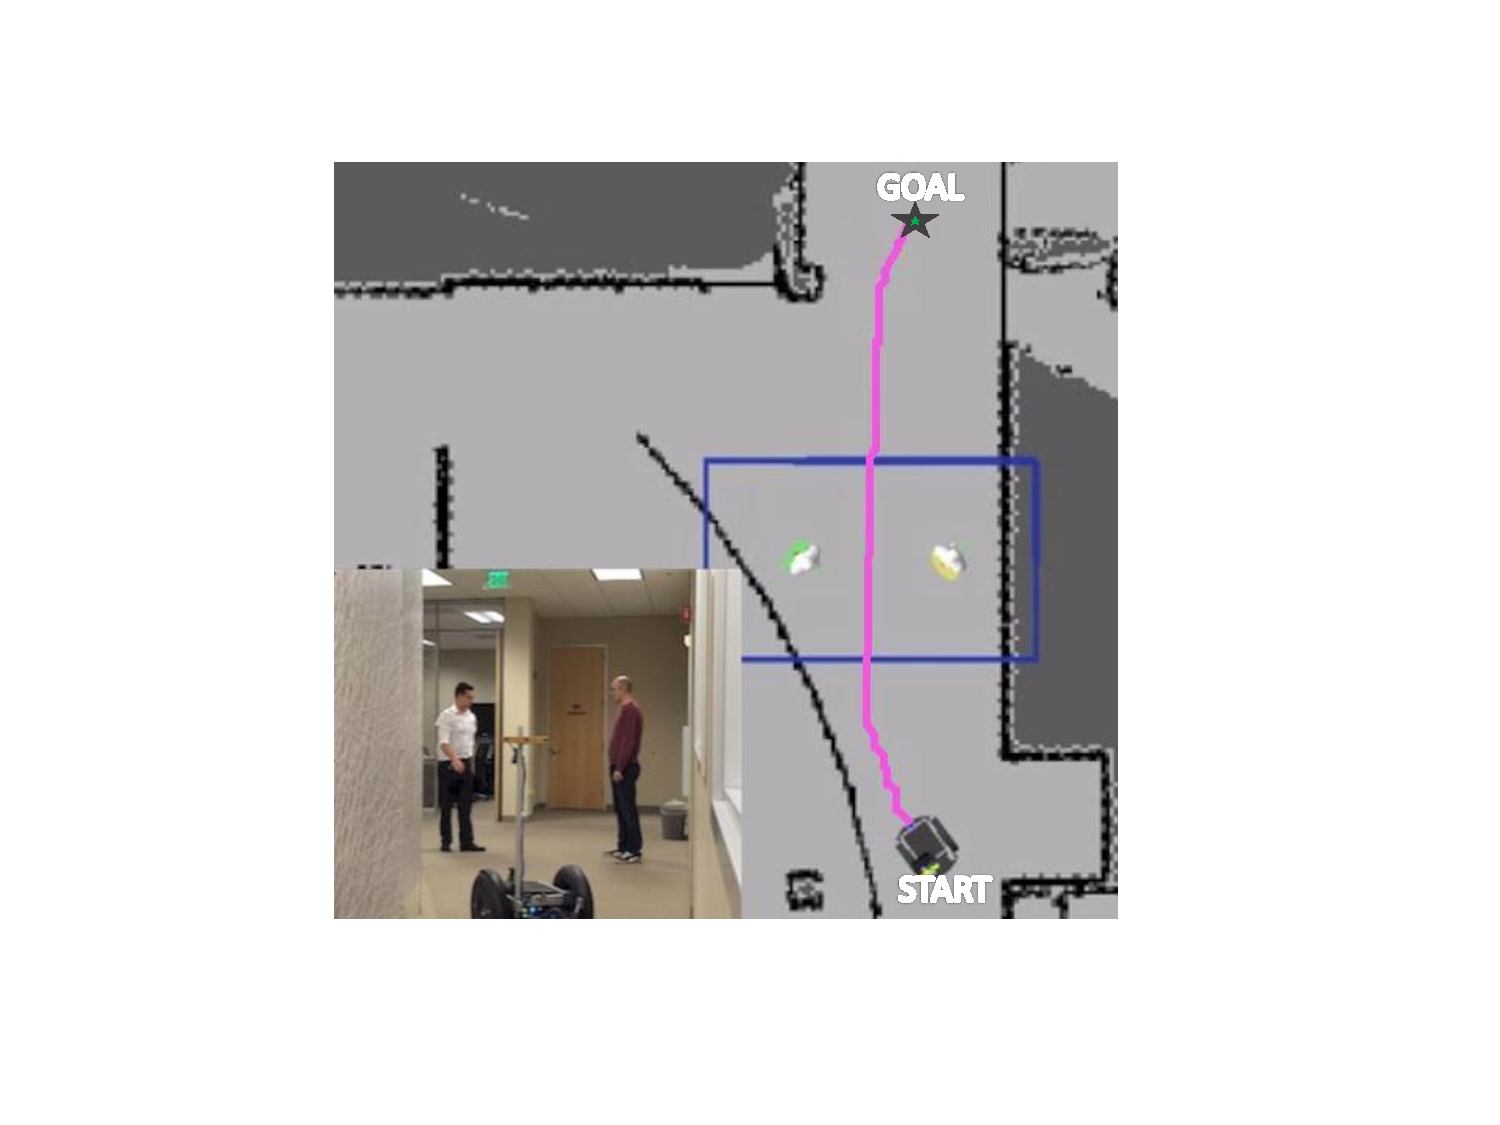
\includegraphics[width=0.58\columnwidth/2]{pics/corridor4_crop}
        }
\subfigure[]{%
           \label{fig:corridor5}
           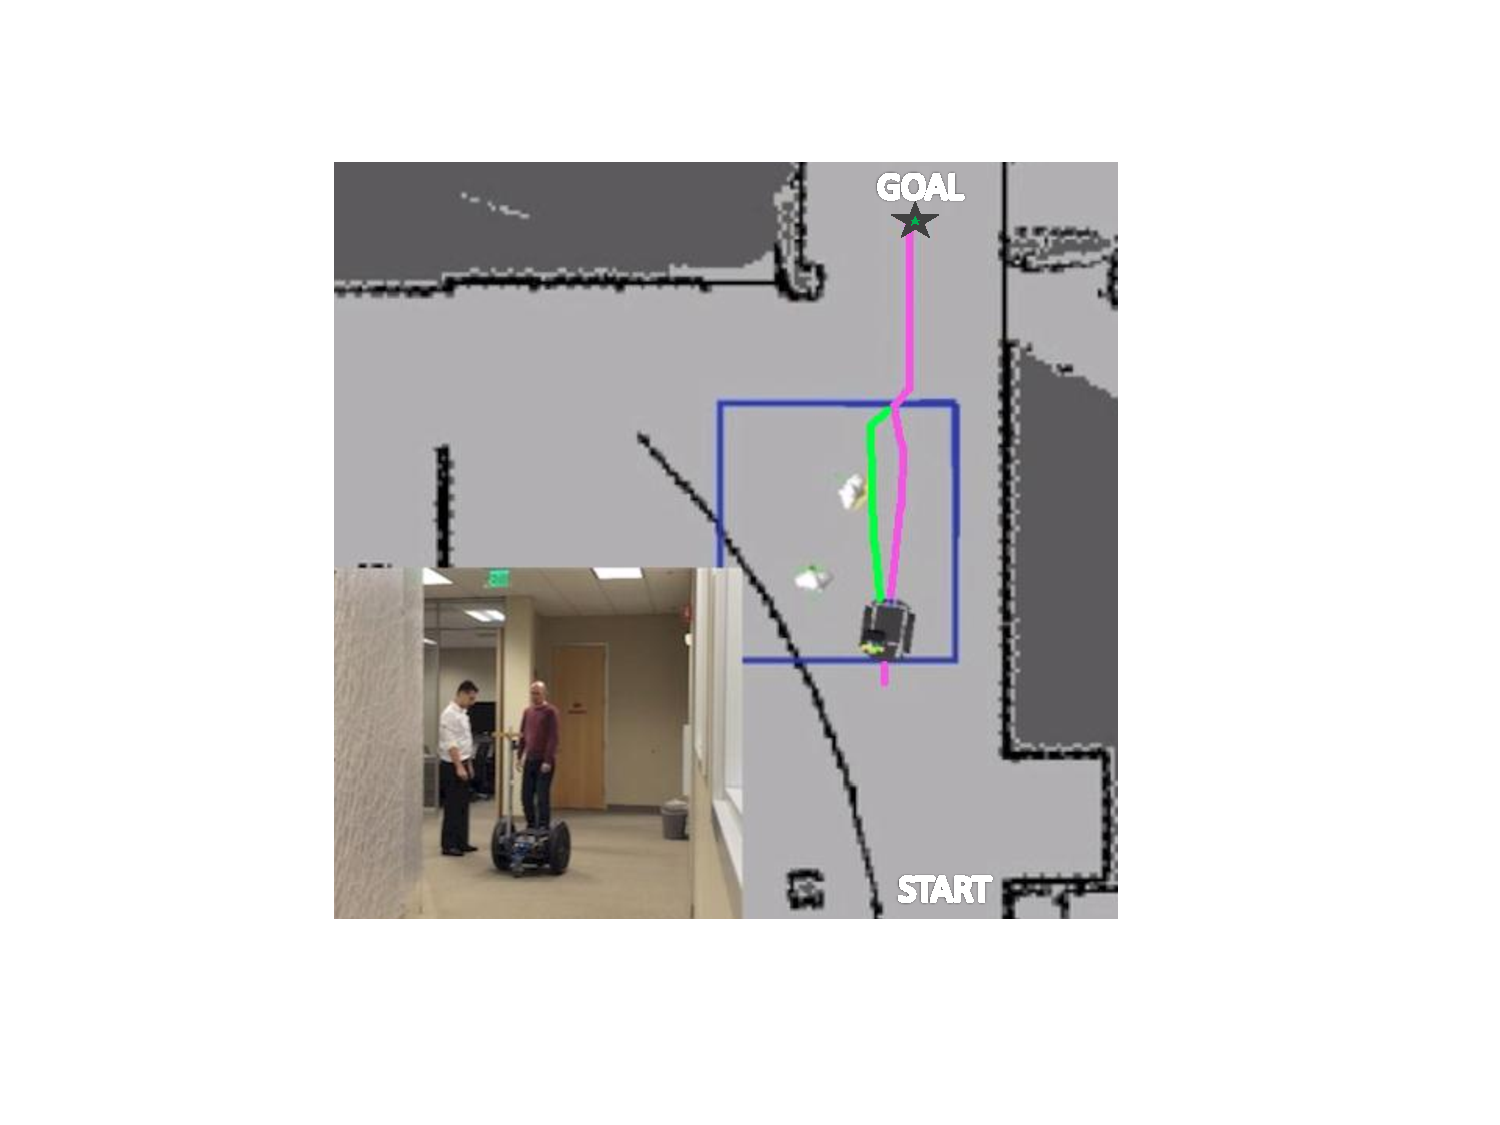
\includegraphics[width=0.58\columnwidth/2]{pics/corridor5_crop}
        }
\subfigure[]{%
           \label{fig:corridor6}
           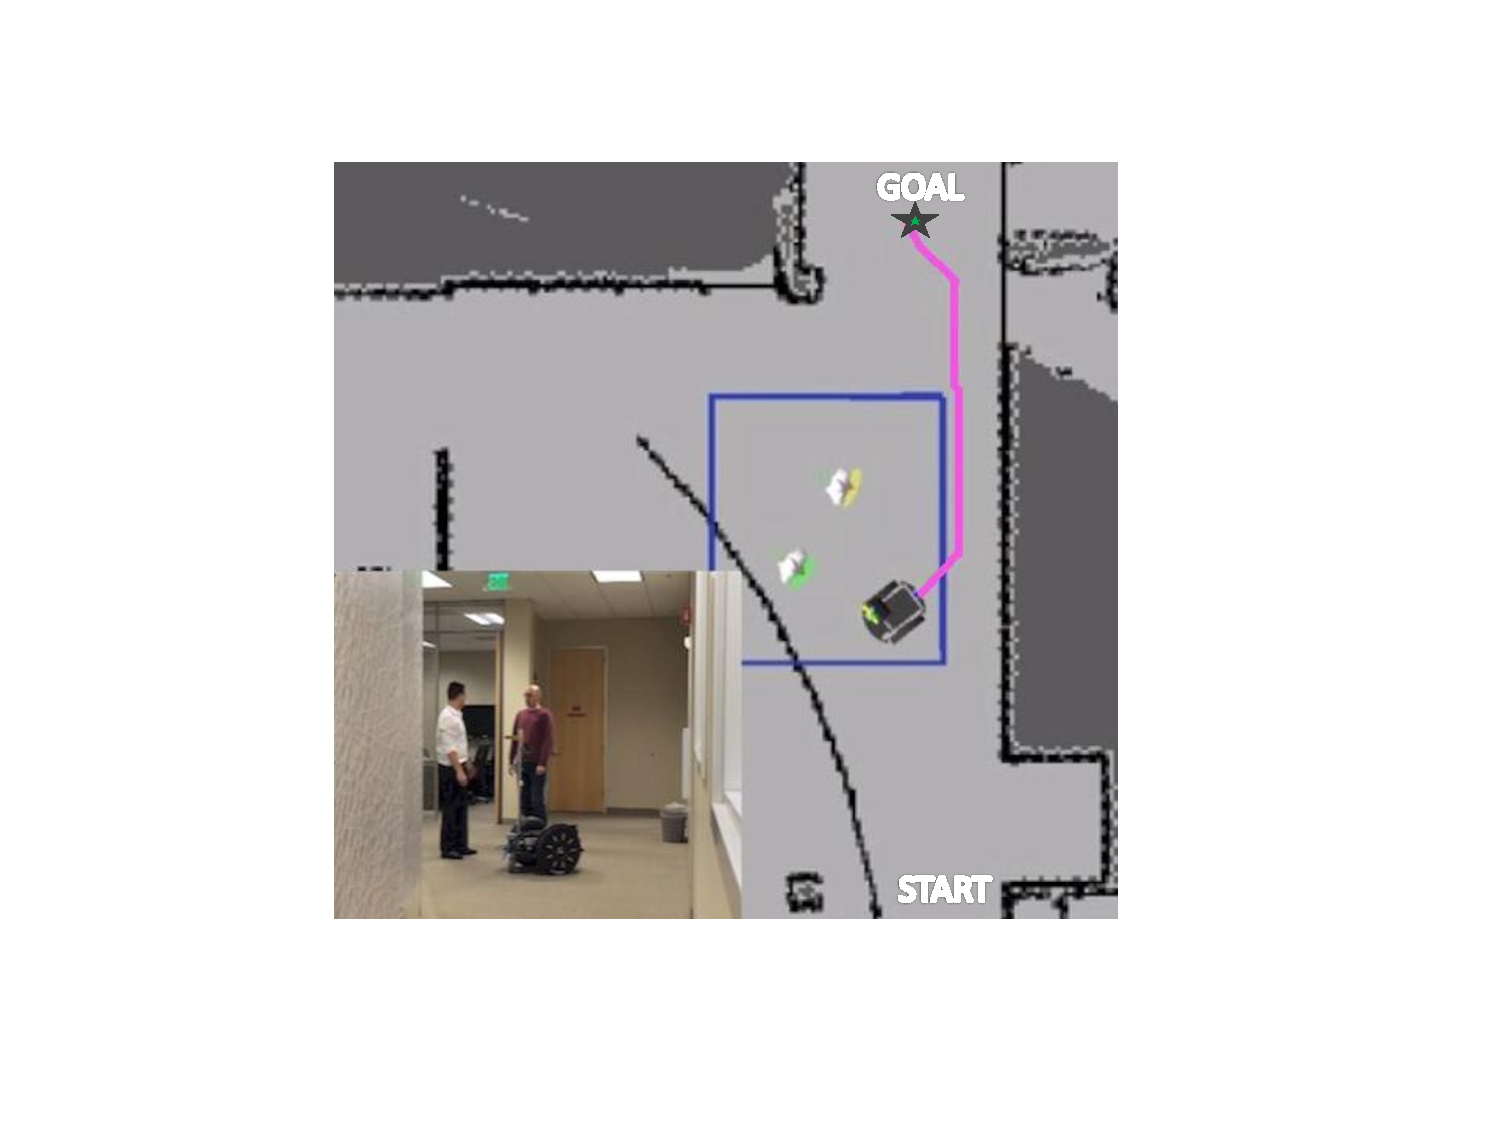
\includegraphics[width=0.58\columnwidth/2]{pics/corridor6_crop}
        }
    \caption{%
	The Hallway scenario. 2 runs are shown in first and second rows.The static plan (green line) and dynamic plan refinement (pink line) are shown. First run: a) Navigation starts. The dynamic planner anticipates that people will give way to the robot when it starts to move towards them. b) Humans notice the robot, and give way by increasing the separation between them. c) The robot continues towards its goal and humans regroup. Second run: d) both the static and dynamic plan involves going in between humans again e) human on the right gets closer to the other person. Since a human made significant movement, dynamic planner re-plans. Plan no longer involves going in between. f) static planner periodic re-plan triggers, leading to robot to stick to the wall to the right.
     }%
   \label{fig:corridor}
\end{figure}


\begin{figure}[p!]
\centering
%
        \subfigure[]{%
            \label{fig:corridor1}
            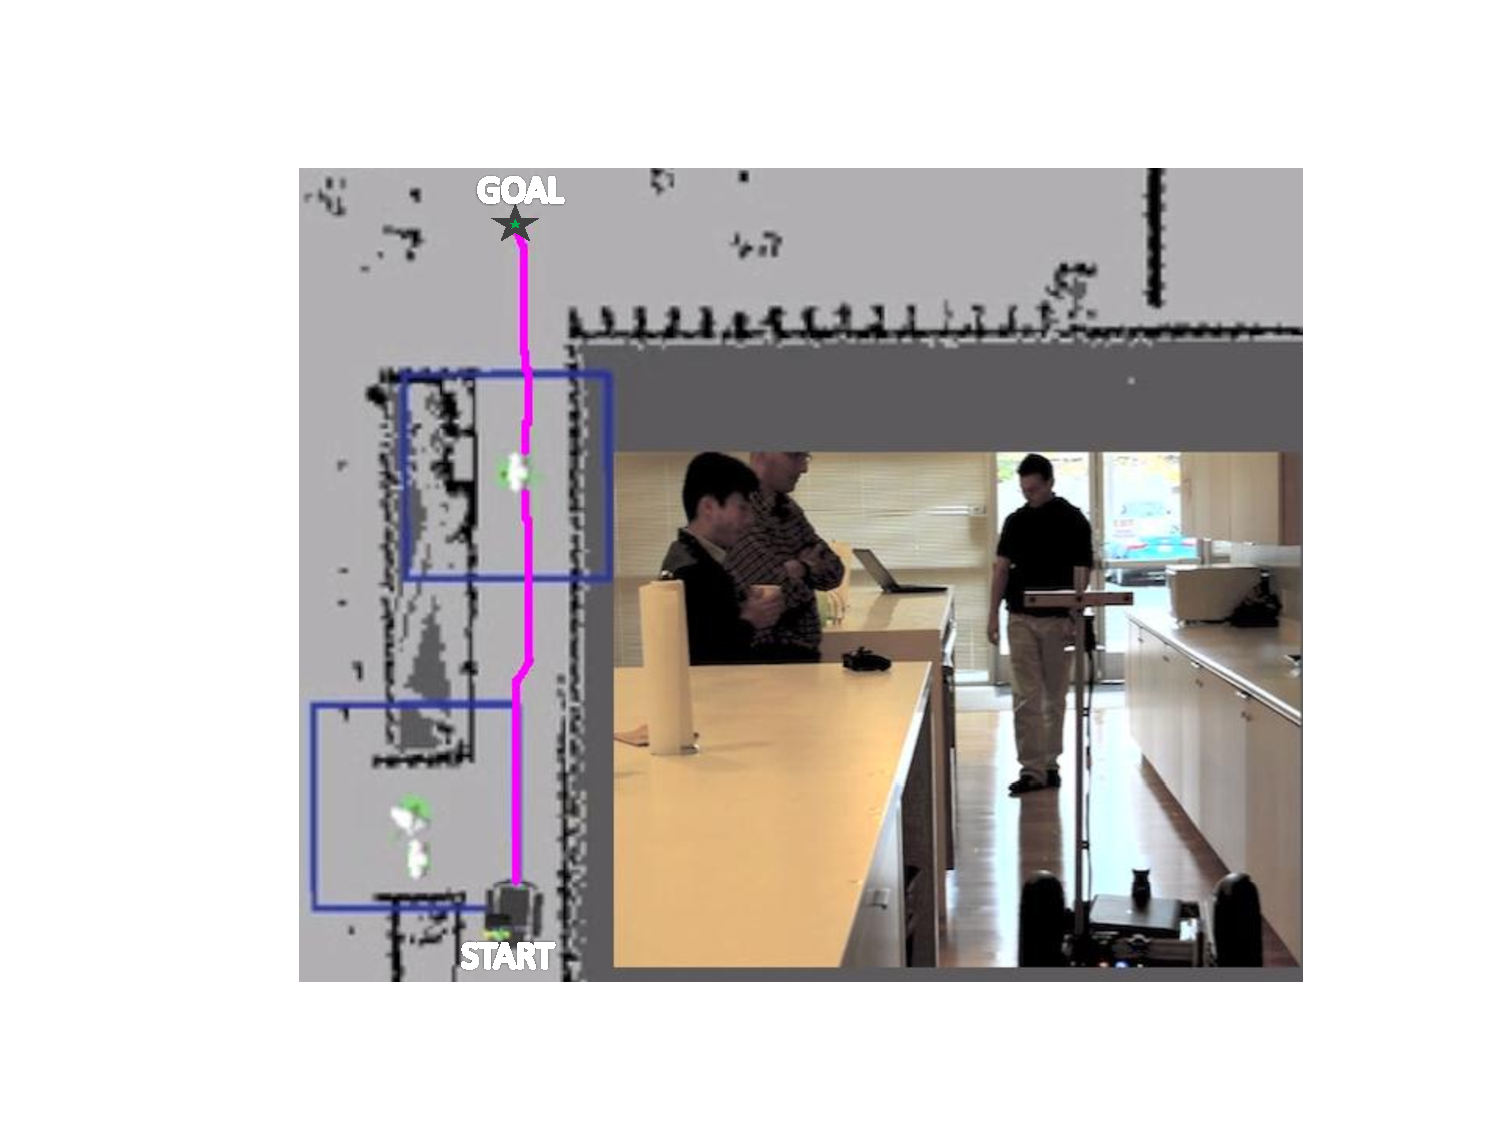
\includegraphics[width=0.6\columnwidth/2]{pics/kitchen1_crop}
        }%
        \subfigure[]{%
           \label{fig:corridor3}
           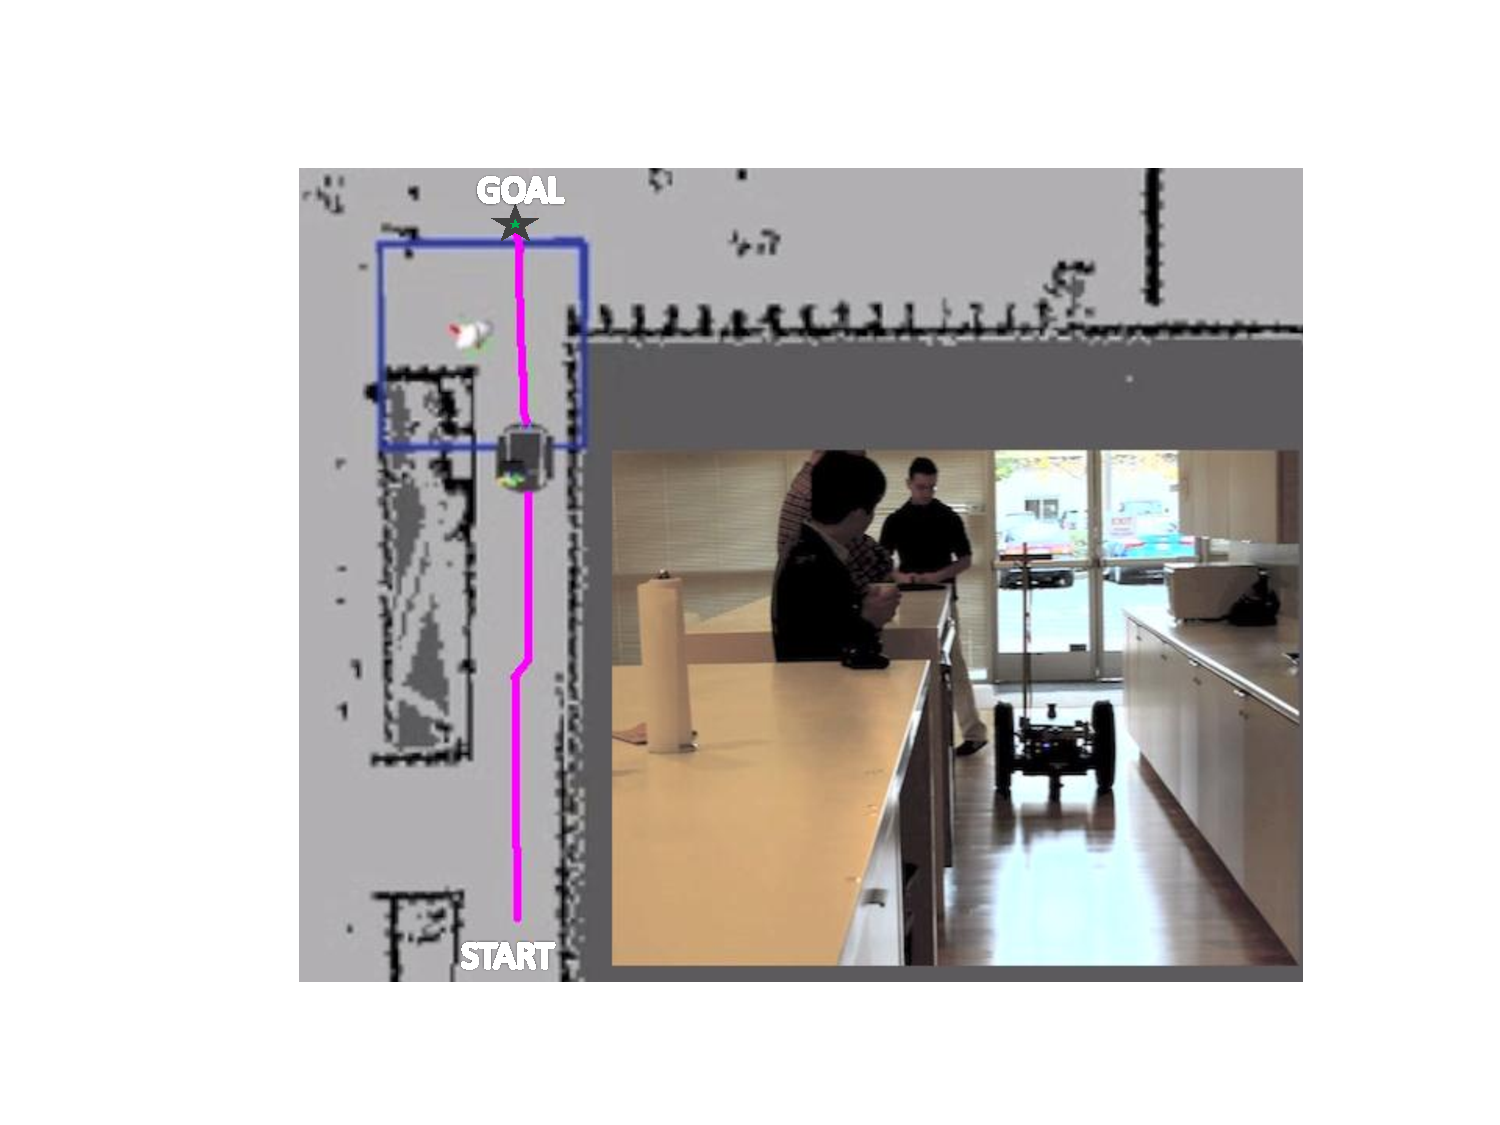
\includegraphics[width=0.6\columnwidth/2]{pics/kitchen3_crop}
        }
\subfigure[]{%
           \label{fig:corridor4}
           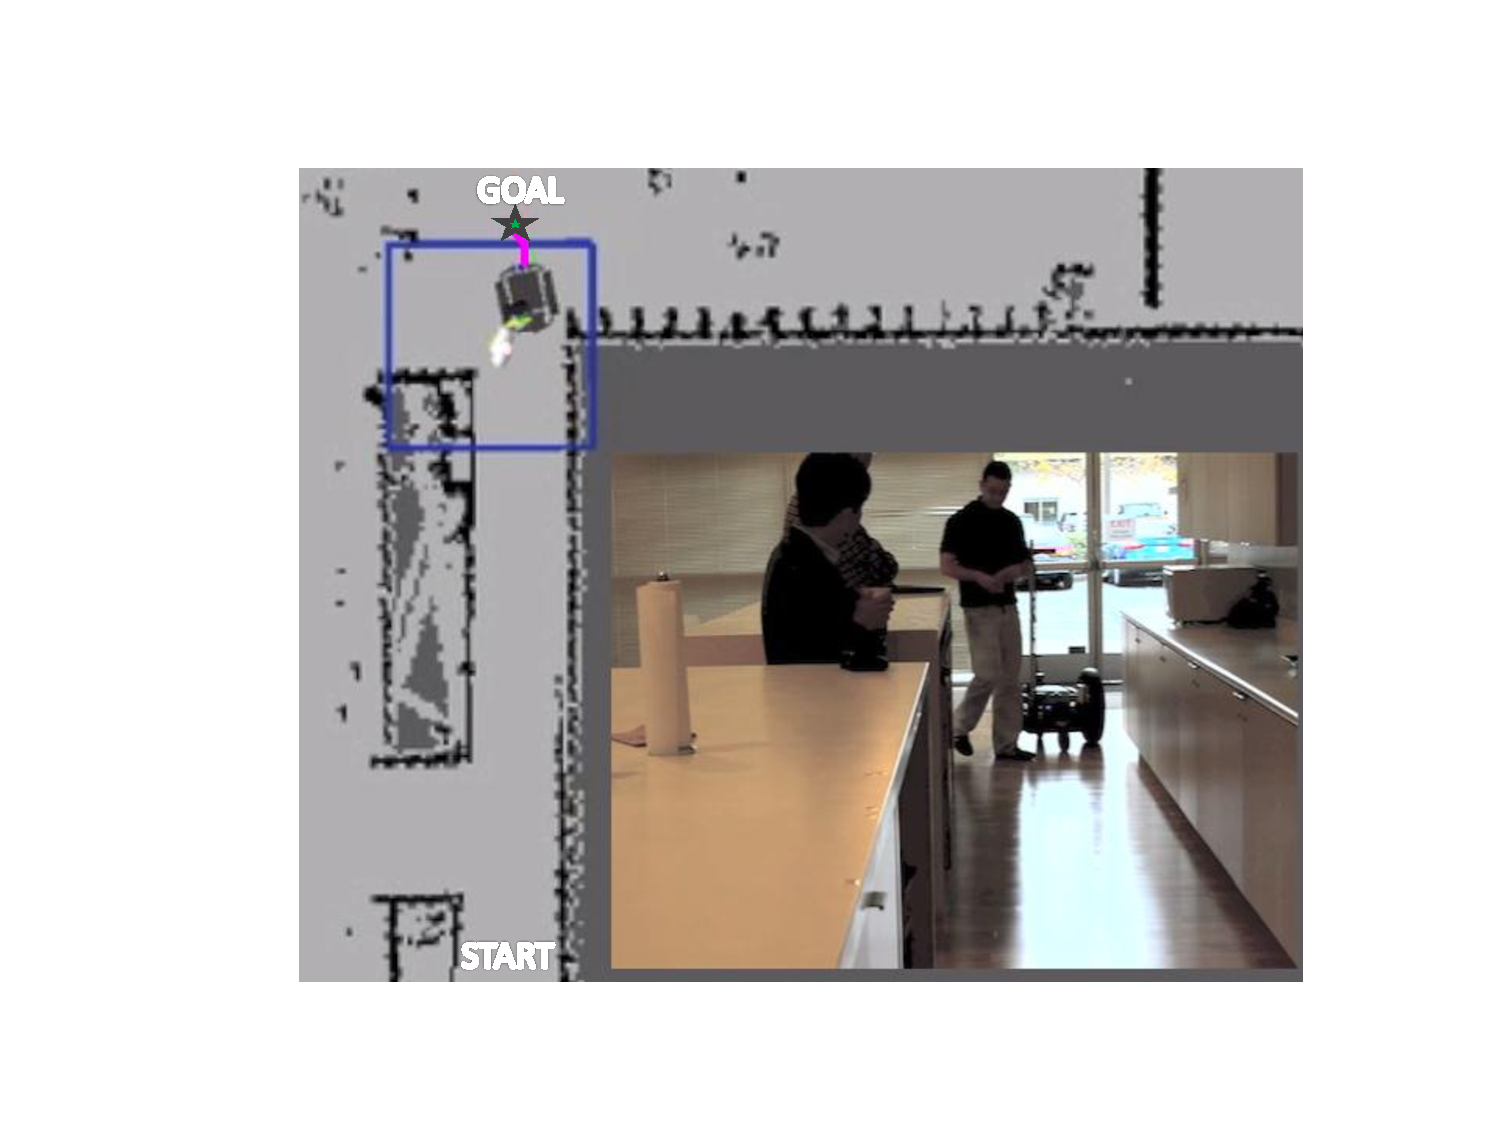
\includegraphics[width=0.6\columnwidth/2]{pics/kitchen4_crop}
        }        
\subfigure[]{%
            \label{fig:corridor1}
            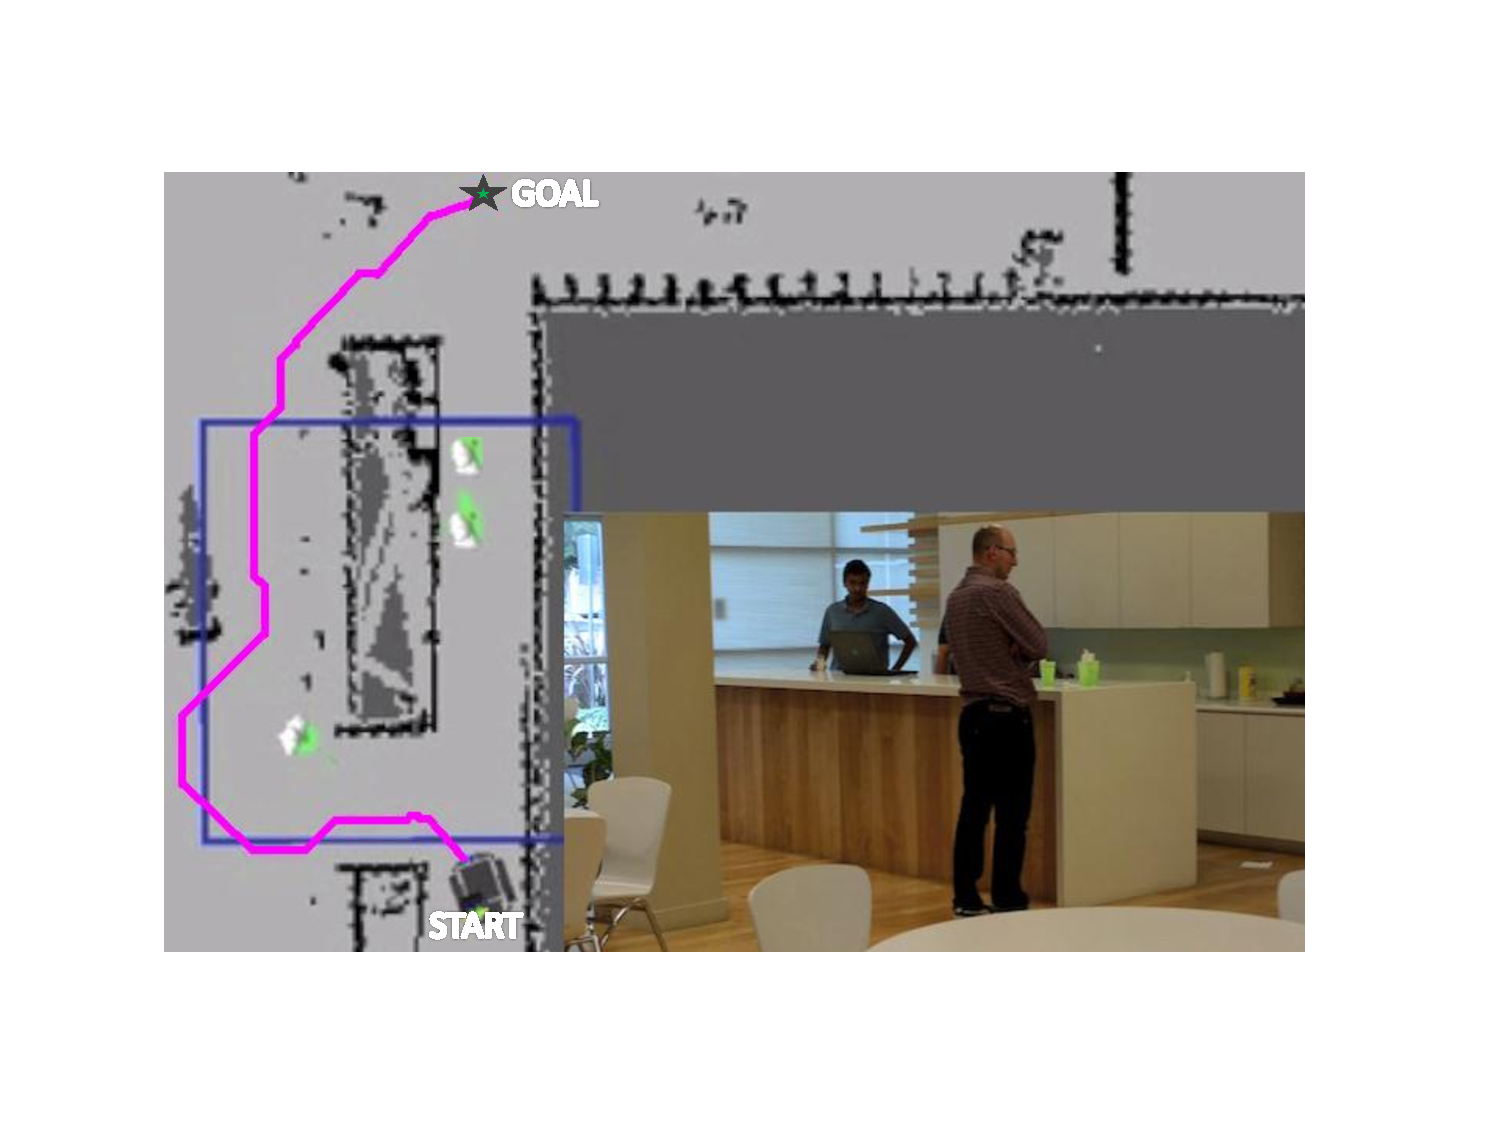
\includegraphics[width=0.6\columnwidth/2]{pics/kitchen5_crop}
        }%
        \subfigure[]{%
           \label{fig:corridor3}
           \includegraphics[width=0.6\columnwidth/2]{pics/kitchen6_crop}
        }
\subfigure[]{%
           \label{fig:corridor4}
           \includegraphics[width=0.6\columnwidth/2]{pics/kitchen7_crop}
        }
        
    \caption{%
	The Kitchen scenario. In the first run, there are two people blocking the path to the left and one person at the narrow corridor. a) robot decides to take the shorter route, because it would disturb one person instead of two. There is not enough space to pass, and dynamic planner assumes the person would get out of the bottleneck to give way. b) human behaves as robot anticipated and gets out of the narrow passage. robot slows down because it enters the human region. c) person gets back to his original position, robot reaches the goal. In the second run: d) there are two people at the narrow corridor and one person on the left. The robot decides to take the longer route and pass the third person from left. The safety cost from the two others would be too high if the robot took the direct route. e) the person steps back as he recognizes the robot. since the person has moved, the dynamic planner re-plans and decides to pass from right. f) after the robot passes the person, it proceeds to its goal.
     }%
   \label{fig:kitchen}
\end{figure}






\section{Speed Limits for Safe Navigation}
\label{sec:navigation_speed_limits}

In this chapter so far, we studied navigation planning that aims to generate human-friendly paths and safety of people must be at the utmost importance. In order to ensure the safety of people, we introduced \textbf{Safety Cost} in Section \ref{sec:navigation_global_planner} as well as repulsion forces in Section \ref{sec:navigation_path_refinement}. However, a seemingly safe path generated by our approach can still lead to an accident because it is may not be possible for the robot to track every human in the environment all the time. For example, when the robot is turning a corner, there is a risk that the robot suddenly encounters a person. Since the robot have finite deceleration, a collision may be unavoidable. The speeds that mobile robots should exhibit is also dependent on the context. For instance, a robot should move slowly and carefully in a hospital room. On the other hand, the robot may navigate faster in a long office corridor. The speed limits should better be provided by experts or the building owners, who govern how fast the robots should navigate in a particular environment.

In this section, we introduce speed maps that sets the speed limits for mobile robots in an environment. We claim that usage of such speed maps make the robots safer and potentially more efficient. The speed map designed for the second floor of the College of Computing building at Georgia Tech is shown in Figure \ref{fig:speed_map_irim}.

\begin{figure}[h!]
\centering
\includegraphics[width=0.6\textwidth]{pics/intro}
\caption{Designed speed limits for. The robot has to be relatively slow in red zones, can have moderate speed in yellow zones and is allowed to move relatively faster in green zones.}
\label{fig:speed_map_irim}
\end{figure}

The free spaces in this map are divided into three zones:
\begin{enumerate}
\item Green zone: The robot is allowed to travel at relatively faster speeds.
\item Yellow zone: Human interaction is possible, top speed is less than the maximum allowed
\item Red zone: Human encounter is probable, top speed is severely limited.
\end{enumerate}

This speed map is designed by hand using the following rules: Spaces corresponding to rooms and cubicles are covered as Red Zones. Blind corners are covered with a Red Zone close to corner and Yellow zone enclosing the Red Zone. Corridors are covered as Green Zones and the rest is covered as Yellow Zones. 

The speed map depicted in Figure \ref{fig:speed_map_irim} is designed by hand, however the speed map generation can be automatized using automatic room categorization and additional processing. Room segmentation has been proposed in an interactive fashion by \cite{diosi2005interactive}, as well as automatically, especially for creating topological maps \cite{mozos2007supervised}.

\subsection{Results}
\label{sec:navigation_speed_maps_results}

In this section, we evaluate the effect of applying speed limits in a navigation scenario. The robot is in an office environment and it has to turn a corner to reach the its goal. There is a person standing right around the corner and the person is not visible to the robot until it gets fairly close to the person. We had two conditions of speed limits:

\begin{itemize}
\item Condition 1: Fixed maximum linear speed of $v_{max}=1.0m/s$
\item Condition 2: Variable speed limits are used according to the speed map: $v_{max}(green)=1.5m/s$, $v_{max}(yellow)=0.5m/s$, $v_{max}(red)=0.15m/s$
\end{itemize}

In both conditions, standard ROS Navigation is used, which found the lowest cost path on a costmap consisting of costs from nearby obstacles. The robot detected the person using our multimodal person detection and tracking method described in Chapter \ref{chapter:multimodal_person_detection_and_tracking}. We analyze the distance/velocity of the robot as it encountered the human and measure the time to reach to the goal as evaluation metrics.

The section of the speed map including the corner is shown in Figure \ref{fig:nav_speed_map_corridor}. The trajectory with a fixed maximum speed is shown in Figure \ref{fig:nav_speed_map_black}. Note that the robot got dangerously close to the human while it turned the corner in Condition 1 and it was traveling with about $0.3m/s$ when it detected the person. The trajectory using the proposed speed limits is shown in Figure \ref{fig:nav_speed_map_color}. With this approach, the robot slowed down as it approached the corner, therefore allowing earlier detection of the human. The robot gave more space to the human in this case, the speed of the robot when it encountered the robot was  $0.15m/s$, half the speed of fixed max velocity case. Considering the speed of the robot and distance to the human at the time of encounter, we can say that the robot was safer.

The second metric we measured was the time to reach the goal. The robot was more efficient with the proposed approach, reaching the goal in $28s$ compared to $29.1s$.



\begin{figure}[ht!]
\centering
%
        \subfigure[]{%           
           \label{fig:nav_speed_map_corridor}
           \includegraphics[width=0.5\textwidth]{pics/speed_map_corridor_pdf}
        } \\
        \subfigure[]{%
        	\label{fig:nav_speed_map_black}
            \includegraphics[width=0.5\textwidth]{pics/nav_noncolor_cropped}
        }%\\        
        \subfigure[]{%           
           \label{fig:nav_speed_map_color}
           \includegraphics[width=0.5\textwidth]{pics/nav_colorr_cropped}
        }
    \caption{Comparison study of using a maximum top speed versus using location-dependent speed limits. Robot is given a fixed goal location. Right around the corner, there is a bystander human, who is not visible to the robot until the robot makes the turn. Points annotate robot position measured at fixed time intervals. a) Speed map of a corridor intersection at the second floor of College of Computing at Georgia Tech. b) Robot's top speed is fixed at $1.0m/s$. Note that the distance between robot positions are mostly constant. The robot gets very close to the bystander because it is moving relatively fast when it turned the corner. c) The robot is allowed to move with $1.5m/s$ in green, $0.5m/s$ in yellow and $0.15m/s$ in red zones. Colors of the sampled points on the path show the associated speed zone. It can be seen by looking at robot's positions that this approach was more gracious turning the corner and respecting human's personal space.}
   \label{fig:nav_speed_map_results}
\end{figure}

%%%%%%%%%%%%%%%%%%%%%%%%%%%%%%%%%%%%%%%%%%%%%%%%%%%%%%%%%%%%%%%%%%%%%%
%%%%%%%%%%%%%%%%%%%%%%%%%%%%%%
\chapter{Person Guidance}
\label{chapter:person_guidance}

The application of guiding a person to a location with a robot has many uses, such as giving tours in museums, showing a visitor locations or individuals of interest and helping the elderly or the visually impaired go to places. We think the guidance behavior is one of the most fundamental capabilities a socially interactive robot should have.

A straightforward approach to guide a person would be the the stop-and-wait method: robot plans a path and executes it normally as long as the guided person is nearby, and stops then the person is outside the radius. However, this method of guidance may lead to sudden stops and would not be socially accepted. A guide robot should consider the distance to the human and incorporate this information in its control strategy.

In this chapter, after reviewing the literature on guide robots in Section \ref{sec:guidance_related_work}, in Section \ref{sec:guidance_guide_robot} we present our guidance method, which adjusts the speed of the robot as a function of the distance to the person. Then we present a special scenario for guidance in Section \ref{sec:guidance_blind_users}, specifically tailored to be used by blind people.

\section{Related Work}
\label{sec:guidance_related_work}

The earliest works in guide robots focused on the implementation and long-term deployment of tour guide robots in public places such as museums. Burgard \cite{burgard1998interactive} presents the robot Rhino, that was deployed to a museum for $47$ hours. The Minerva robot was an improved model over Rhino \cite{thrun1999minerva}, and was deployed to a museum with an order of magnitude larger floor space. This robot was in operation for two weeks, and it was able to have short-term interaction with people , i.e. head motion, facial expressions. Siegwart \cite{siegwart2003robox} presents a robot that was deployed to an exhibition for 6 months. Nourbakhsh \cite{nourbakhsh2003mobot} presents a project where four guide robots were deployed to museums for a period of five years. The authors remark that it is indeed possible to deploy guide robots public places, unsupervised. All these tour-guide robots had various degrees of autonomy and was received with enthusiasm. However, in all of these works it was apparent that there is a need for research in the area of Human-Robot Interaction.

Pacchierotti \cite{pacchierotti2006design} demonstrates an office guide robot, but the main focus is on passing people in corridors. Clodic \cite{clodic2006rackham} presents another robot deployed in a museum. It was reported that a continuous interaction all along the guiding mission is fundamental to keep visitor's interest. Martin \cite{martin2004conception} studies the scenario of guiding a visitor in an office environment and focuses on robust person tracking. Pandey \cite{pandey2009step} focuses on the leave-taking of the guided person. The robot predicts the intent of the discontinuation of the task and either breaks the mission or searches for the user depending on the waiting time. Martinez-Garcia \cite{martinez2005crowding} focuses on the scenario of guiding a group of people with multiple robots at the same time. Garrell \cite{garrell2010local} works on a similar problem, where the task of the two robots is to control group of people and guide them. Another relevant scenario is the evacuation scenario, in which there is a danger and robots guide people to the safe a location \cite{kim2009portable,robinette2011incorporating}.

\section{Guide Robot}
\label{sec:guidance_guide_robot}

In this section, we describe our method of person guidance. After a request to guide a person is received from a higher level process, the robot first plans a path using our navigation planner in Section TODO, or standard ROS Navigation. The robot continues on its path as long while constantly monitoring the distance between itself and the guided person. The robot adjusts its speed according to this distance. 

We use a variable speed profile so that the robot can better keep up with the person and the motions of the robot is smoother. We define a speed function that is a function of the distance between the robot and the user. This speed profile is shown in Figure \ref{fig:guidance_speed_profile}. The robot moves at a low speed $v_{safe}$ if the human is dangerously close. The speed is peaked at distance $d_{peak}$ and the robot stops if the distance is larger than $d_{guide}$, which may indicate that the human is not interested in being guided. Note that $v_{peak}$ is capped by the speed limits in the environment, provided by the speed map approach presented in Section TODO.

\begin{figure}[ht!]
\centering
\includegraphics[width=0.5\textwidth]{pics/speed_profile_cropped}
\caption{Speed profile of a person guiding robot as a function of the distance to the user.}
\label{fig:guidance_speed_profile}
\end{figure}

In the second scenario, the robot has the same goal point and guiding a person. In the first condition, we use ROS Navigation but robot stops if the distance to the human is over a threshold. In second condition, we use our method of dynamic speed adjustment for guidance. In this scenario, there is no person standing around the corner. We measured the instantaneous speeds of the robot and the human.


\subsection{Results}
\label{sec:guidance_results}

The robot is given a fixed goal to guide a person, who is tracked with a torso-level laser scanner, by fitting an ellipse to the torso. We compared the velocity profile in Figure~\ref{fig:guidance_performance_graph} with $d_{guide}=1.7$m, $d_{peak}=0.9$m, $d_{safe}=0.1$m, $v_{safe}=0.1$m/s, $v_{peak}=1.0$m/s. We compared our approach with the simple strategy: If the human is closer than $d_{guide}$, then the navigation continues with a fixed max speed. Otherwise robot stops and waits.

\begin{figure}[ht!]
\centering
%
        \subfigure[]{%
        	\label{fig:guidance_graph_noadj}
            \includegraphics[width=0.75\textwidth]{pics/graph_noadj}
        }%\\
        
        \subfigure[]{%           
                	\label{fig:guidance_graph_adj}
           \includegraphics[width=0.75\textwidth]{pics/graph_adj}
        }        
    \caption{%
	Comparison of robot and human speeds with respect to time. a) Standard ROS Navigation b) Our approach: accelerations are less steeper than a), which employs the dynamic speed adjustment for guidance.
     }%
   \label{fig:guidance_performance_graph}
\end{figure}

In the experiment, when guiding was enabled, the human first waited until the robot stopped at $d_{guide}$. Then he took a step and waited for a second time, and then started following the robot. The comparison of robot speeds is given in Figure \ref{fig:guidance_graph_noadj} for fixed max speed and Figure \ref{fig:guidance_graph_adj} with the speed profile. Between $t=0$ and $t=9s$, the accelerations are much more rapid for the fixed max speed case. Robots that exhibit high accelerations will likely be perceived as unsafe, therefore our approach exhibits a more socially acceptable behavior. Moreover, after the person started following ($t >9s$), our approach is better at mimicking the speed of the human.


\section{Application To Blind Users}
\label{sec:guidance_blind_users}

In this section, we present our person guidance system specifically tailored for guiding blind users. Our approach consists of planning a path for the user and applying vibrations via a haptic belt to keep the user on the path.

%System graph, persception ellipse

\subsection{Tactile Belt}

In the previous section, we assumed that the guided person can detect where the robot is and follow him/her. With a blind user, this assumption does not hold. Therefore we need a mechanism to give directions to the user. Readily available options for assistive interfaces are limited to Braille or devices that presents content with speech synthesis. These ways of presenting information have difficulty dealing with representing spatial information. We also think visually impaired individuals would prefer a non-speech interface because they mostly rely on their sense of hearing in daily life. We therefore use a tactile belt for navigation guidance, because it can represent directions and rotations, be worn discreetly and does not occupy the hearing sense.

The belt has 8 pancake vibration motors, linearly spaced around the waist, and the motors can be controlled asynchronously via an Arduino board. We used two distinct vibration patterns to control the person's movements:

\begin{enumerate}
\item Directional Movement: When the guided person should move in a direction
\item Rotational Movement: When the guided person should turn around self
\end{enumerate}

The vibration patterns that induce directional and rotational movements in the human can be specified in many ways. We evaluated four patterns in each category with a user study. The details of this user study as well as a survey about the usability of the Tactile Belt is provided in Appendix TODO. The user study showed that the directional motion pattern with the highest recognition rate and least reaction time was the \textbf{TWO TAPS} pattern, which is illustrated in Figure TODO. For the rotational motion pattern, we used the continuous rotation with a single motor, illustrated in Figure TODO. 

\begin{figure}[ht!]
\centering
\includegraphics[width=1.0\textwidth]{pics/vibration_pattern_two_taps}
\caption{The vibration pattern applied by the Tactile Belt to induce directional movements in the blind user. A motor is fired for a duration of $250ms$, inactivated for $250ms$ and fired again for $250ms$.}
\label{fig:vibration_pattern_two_taps}
\end{figure}

\begin{figure}[ht!]
\centering
\includegraphics[width=1.0\textwidth]{pics/vibration_pattern_solo_cont}
\caption{The vibration pattern applied by the Tactile Belt to induce rotational movements in the blind user. The consequent vibrations motors are fired consecutively, starting from left for CW and right for CCW rotation.}
\label{fig:vibration_pattern_solo_cont}
\end{figure}


\subsection{Planning the Path of the User}

ROS provides an easy-to-use navigation stack for mobile robots. The input to the navigation stack is a map and a goal point and the output is a path and linear and angular velocities \emph{(v,w)} necessary to keep the robot on the course of the path. We assumed that the human is a non-holonomic robot with a circular footprint. The obstacle information is acquired from the laser scanner and the goal is provided in the sensor frame. Coupled with the Human Tracker, the 'robot' stays localized in the map and with respect to the path. The path is re-planned every second to deal with possible deviations. Next section is concerned with how the linear and angular velocities are converted to the vibration patterns.

\subsection{Velocity to Vibration Mapping}


Given a desired velocity that the 'robot' should execute, we first determine if a directional or rotational vibration pattern should be applied by the belt. If the linear velocity is dominant, then the human should walk towards that direction. If the angular velocity is dominant, the human should rotate around self. If both the linear and angular velocity is close to zero, the human should not move. To calculate which motion is appropriate, the 'robot' is simulated using Equation TODO. If the distance the 'robot' took is larger than a threshold, then a directional vibration pattern is used. If it is less than the threshold, a rotational pattern is used. If both of the velocities are small enough, the no vibration is applied. 

When the human gets to the vicinity of the goal point, a special stop signal is applied to inform the person that the destination is reached. Stop signal is implemented similar to \textbf{TWO TAPS} pattern except all the motors are activated instead of one.

\subsection{Demonstration}

We demonstrated that our system can successfully guide a blindfolded person to a goal location in a room. Based on our evaluation results of vibration patterns, we used \textbf{CONT} for directional motions and \textbf{SOLO CONT} for rotational motions. The experimenter manually provided several goal poses using the GUI. Note that since the system is re-planning frequently, the planner is able to accommodate dynamic obstacles and compensate unpredictable motions of the person. The demonstration steps as well as their explanations are shown in Figure~\ref{fig:blindguidepics}.

\begin{figure*}[ht!]
\centering
%
        \subfigure[]{%
            \label{fig:blindguide1}
            \includegraphics[width=0.45\columnwidth]{pics/blindguide1}
        }%
        \subfigure[]{%
           \label{fig:blindguide2}
           \includegraphics[width=0.45\columnwidth]{pics/blindguide2}
        }
        \subfigure[]{%
           \label{fig:blindguide3}
           \includegraphics[width=0.45\columnwidth]{pics/blindguide3}
        }
\subfigure[]{%
           \label{fig:blindguide4}
           \includegraphics[width=0.45\columnwidth]{pics/blindguide4}
        }
\subfigure[]{%
           \label{fig:blindguide5}
           \includegraphics[width=0.45\columnwidth]{pics/blindguide5}
        }
\subfigure[]{%
           \label{fig:blindguide6}
           \includegraphics[width=0.45\columnwidth]{pics/blindguide6}
        }
    \caption{%
	Autonomous guiding of a blindfolded person using the tactile belt. a) The guidance starts. The user is blindfolded and is standing at the left of the screen. The human detection system detects him and places an ellipse marker with an arrow depicting his orientation. The operator gives a goal point by clicking on the screen. The goal point is the right traffic cone, and given by the big arrow. b) The system autonomously generates a path for the user. As seen in the picture the path is collision free. At this stage the belt begin to vibrate towards the front of the user. c) An unexpected obstacle (another person) appears and stops in front of the user. The system detects the other person as an obstacle, and reevaluates the path. A new path going around the obstacle is immediately calculated and sent to the user by the belt. d) The user receives a rotation vibration modality, and begins to turn towards the new path. And follows this path from now on. e) The obstacle leaves. The path is then reevaluated and changed. The user receives forward directional belt signal, and advances towards the goal. f) The person reaches to the vicinity of the goal and stop signal is applied.
     }%
   \label{fig:blindguidepics}
\end{figure*}

%%%%%%%%%%%%%%%%%%%%%%%%%%%%%%%%
\chapter{Situation Aware Person Following}
\label{chapter:following_situation_aware}

Simply put, \textit{Situation Awareness (SA)} is knowing what is going on around you. Endsley \cite{endsley2000situation} defines three steps for SA: perception, comprehension and projection. Perception is detecting the situation by perceiving cues, comprehension is combining and interpreting information and projection is forecasting future events. In this section, we discuss SA for person following behavior for mobile robots. In the Chapter \ref{chapter:person_following}, we presented the basic following behavior, where the robot follows the person strictly from behind, while maintaining a fixed distance. The related works on person following discussed in Section \ref{sec:following_related_work} mostly use the same principle: the robot uses the person to calculate a target position and blindly follows the human irrespective of the situation. Although this method is sufficient for some scenarios, it can easily lead to socially awkward situations. For example, consider the case that the followed person stops just outside a door. In this case, the robot would occupy the doorway, blocking other people's passage, however thinks it is doing its task well because it maintains a fixed distance to the user. If the robot knows what the user intends to do, it can anticipate those actions and suitably adjust its behavior. Person following can be used in different contexts, such as for carrying luggage in airports or groceries in a supermarket. We showed in Chapter \ref{chapter:map_annotation} that semantic maps that include landmarks and waypoints could be used to communicate goals between the robot and the user.  The stored semantic information can also be used to facilitate robot navigation. We specifically focus on three scenarios of situation aware person following:

\begin{enumerate}
\item Joining a group of people
\item Labeling landmarks during the Tour Scenario
\item Passing Doors
\end{enumerate}

The robot behaviors for each of these scenarios are modeled and executed via triggered events, inspired by Cakmak's framework \cite{cakmak2011using}. Handling of an event during following is implemented as a sequence of four phases:

\begin{enumerate}
\item Signal: Robot detects an event using perceptual cues
\item Approach: Robot moves to a position better suited to the task
\item Execution: Robot and/or Human execute the task
\item Release: Robot detects the end of event and continues with the basic following behavior
\end{enumerate}

With this methodology, robot uses the three steps of SA: Perception for detecting the start and ending of an event, Comprehension for interpreting where it should move to and what the task is, and Projection to estimate the future goals of the person. In this chapter, we study three scenarios that could be encountered while the robot is following the person. In Section \ref{sec:following_joining_group}, we first show how the robot moves when the followed person stops and talks with someone else. In Section \ref{sec:following_landmark_labeling}, we study the following behavior for labeling landmarks during the Tour Scenario. In Section \ref{sec:following_door_passing}, we look at how the robot should handle door passages.


\section{Joining a Group}
\label{sec:following_joining_group}

While the robot is following a person, one of the scenarios that could be encountered is when the followed person interacts with some other person. If the basic following method is used, the robot would stay behind the person and that could lead to an awkward formation where the robot is left out of the group (see Figure \ref{fig:group_problem} for an example). Our proposed solution to this problem is for the robot to join the group of people using engagement rules. Joining a group has been addressed previously \cite{althaus2004navigation,setti2015f}, however not in the person following context.

\begin{figure}[ht!]
\centering
\includegraphics[width=0.5\textwidth]{pics/group_problem}
\caption{The problem that occurs when the followed person stops and interacts with another person is shown. The robot is left out of the group when it does not detect or react to this social situation.}
\label{fig:group_problem}
\end{figure}


Our solution to this problem is to choose a position for the robot to stay during the conversation. Our choice of the position is guided by Kendon's F-Formations \cite{kendon1990conducting}. Kendon studied how people assemble and what formations they assume while they are interacting. In this representation the space is divided in three regions as can be seen in Figure: \ref{fig:keldon}. \textit{o-space} is the empty space surrounded by people,  \textit{p-space} contains the participants and \textit{r-space} is the outer area beyond the \textit{o-space}. Kendon studied commonly encountered formations such as L-formation, circular, face-to-face and side-by-side formations.

\begin{figure}[ht!]
\centering
\includegraphics[width=0.5\textwidth]{pics/keldon}
\caption{Definition of space around people according to Keldon's F-Formation representation of group formations}
\label{fig:keldon}
\end{figure}

In our approach, when the robot detects the existence of a group formation, it samples poses on the \textit{p-space}, scores them and chooses a collision-free goal pose. When the interaction ends and the group formation is broken, the robot continues the basic following behavior. The execution phases for this behavior as well as the behavior transitions are given in Table \ref{table:situation_aware_list_group}.



\begin{table}[ht!]

    \caption{Conditions to trigger phases when the user is involved with the Joining a Group Event during following.}

    \centering
    	
  \begin{tabular}{l |  m{10cm}}    
    \toprule    
    Signal & {$dist(user, groupcenter)<threshold$}\\       
	                           & {$speed(user)\sim 0$} \\
	                           & {person roughly facing group}\\ \midrule		                           		                                
    Approach & {Optimal Goal: in the \textit{p-space} in the circular formation}\\       \midrule
    Execution & {The group interacts with each other, including the robot}\\  \midrule
    Release & {$dist(user, groupcenter)>threshold$}\\ 
    \bottomrule
  \end{tabular}
    \label{table:situation_aware_list_group}
\end{table}

We follow the Signal/Approach/Task/Release procedure for the design of this behavior. The Signaling phase is triggered whenever the user is close to another person or a group of people. The user must have close to zero speed to enable signaling for this behavior, because the user may walk past the group. After the robot detects the signal, we sample positions around the group to locate a ``suitable" goal pose for the robot. A pose that is collision free but that gives the robot highest chance of interaction is favored. We use a utility function that scores candidate goal points. Intuitively, a pose that is close to both people and could see both is considered a suitable goal pose. We sample points $360^{\circ}$ around the \textit{p-space}, for a fixed sampling resolution. 

\begin{figure}[ht!]
\centering
%
        \subfigure[]{%           
           \label{fig:situtation_aware_joining_group_0}
           \includegraphics[width=0.475\textwidth]{pics/group_demo_1}
        } 
         \subfigure[]{%           
           \label{fig:situtation_aware_joining_group_1}
           \includegraphics[width=0.48\textwidth]{pics/group_demo_2}
        } \\
        \subfigure[]{%
        	\label{fig:situtation_aware_joining_group_2}
            \includegraphics[width=0.48\textwidth]{pics/group_demo_3}
        }%\\        
        \subfigure[]{%           
           \label{fig:situtation_aware_joining_group_3}
           \includegraphics[width=0.49\textwidth]{pics/group_demo_4}
        }
    \caption{Demonstration of the robot joining a group when the followed person interacts with a group of people. The robot is initially following the user throughout the environment and keeping a fixed distance of $1.2m$ to the user. a) Signal phase: The user has stopped and is in the cloxe proximity to to another person. b) Approach phase: The robot calculates and navigates to a goal position, so it can potentially interact with people in the group. c) Execution phase: The interaction happens. c) Release phase: user moves away from the group and basic following behavior continues.}
   \label{fig:situtation_aware_joining_group}
\end{figure}

Every sampled position $p$ has a score of:
\[
Score(p) = 1.0 - Cost_{visibility}(p) - Cost_{obstacle}(p)
\]
Where we define the costs as:
\begin{align} 
\begin{split}
Cost_{visibility}(p)&=dist(user,person)/(dist(p,person)-dist(p,user)) \\
Cost_{obstacle}(p)&=max(local\_cost(p),global\_cost(p))
\end{split}
\end{align}

The local and global costs are fetched from the ROS costmaps, normalized to [0.0-1.0] interval. The sample with the highest nonnegative score is chosen as the goal position. The orientation of the robot is chosen as looking toward the center of all the people in the group. After the goal pose is determined, the robot is commanded to navigate there. During the Execution phase, interaction that potentially involves the robot occurs. Whenever the user leaves the group, then the Release phase is executed. The robot continues tracking the user with the basic following method.

This behavior is implemented on a real robot and snapshots from this demonstration is shown in Figure \ref{fig:situtation_aware_joining_group}.

\section{Following For Labeling}
\label{sec:following_landmark_labeling}

One of the problems we found out during the Tour Scenario experiments was that as the robot is following the user, it does not have any information about the task. This leads to awkward situations when the user wants to label a landmark or object, because the robot can not perceive the pointing gesture or the object/landmark of interest at the same time when it is following from behind all the time. This situation is illustrated in Figure \ref{fig:landmark_labeling_example}.

\begin{figure}[ht!]
\centering
        \subfigure[]{%           
           \label{fig:label_ex_1}
           \includegraphics[width=0.58\textwidth]{pics/label_ex_1}
        } \\
        \hspace*{3cm}
         \subfigure[]{%           
           \label{fig:label_ex_2}
           \includegraphics[width=0.38\textwidth]{pics/label_ex_2}
        } 
    \caption{a) A common problem we encountered during the Tour Scenario. The user wants to label an object on the table, however the robot does not understand this intention and stays behind at a fixed distance to the user. b) Our solution is to move to a location that has the visibility of both the user and the object.}
   \label{fig:landmark_labeling_example}
\end{figure}

 The robot behavior can be more intelligent in those cases if the robot can predict ahead of time when the user is going to label landmark. The robot follows the phase transitions defined in Table \ref{table:situation_aware_list_landmark} for this scenario.
 
\begin{table}[ht!]

	\caption{Conditions to trigger phases when the user is involved with the Landmark Labeling Event during following.}
	
		\centering
		
  \begin{tabular}{l |  m{10cm}}
    \toprule    
    Signal & {$dist(user, convex hull(landmark))<threshold$}\\       
	                           & {$speed(user)\sim 0$} \\
	                           & {person roughly facing landmark}\\ \midrule		                           		                                
    Approach & {Optimal Goal: Close to both the landmark and person, facing in between}\\       \midrule
    Execution & {User points and labels landmark}\\  \midrule
    Release & {$dist(user, convex hull(landmark))>threshold$}\\ 
    \bottomrule
  \end{tabular}
    \label{table:situation_aware_list_landmark}
\end{table}


\begin{figure}[ht!]
\centering
%
        \subfigure[]{%           
           \label{fig:situtation_aware_landmark_labeling0}
           \includegraphics[width=0.475\textwidth]{pics/sit_table_00}
        } 
         \subfigure[]{%           
           \label{fig:situtation_aware_landmark_labeling2}
           \includegraphics[width=0.48\textwidth]{pics/sit_table_02}
        } \\
        \subfigure[]{%
        	\label{fig:situtation_aware_landmark_labeling3}
            \includegraphics[width=0.48\textwidth]{pics/sit_table_03}
        }%\\        
        \subfigure[]{%           
           \label{fig:situtation_aware_landmark_labeling4}
           \includegraphics[width=0.49\textwidth]{pics/sit_table_04}
        }
    \caption{Demonstration of situation awareness for the Tour scenario. The robot is following the user throughout the environment and keeping a fixed distance of $1.2m$ to the user. a) Signal phase: The user has stopped and is in the cloxe proximity to the convex hull of the table. b) Approach phase: The robot calculates and navigates to a goal position, so it can perceive the pointing gesture and target. Execution phase: The user points out to the object on the table. c) Release phase: user moves away from the table d) Basic following behavior continues.}
   \label{fig:situtation_aware_landmark_labeling}
\end{figure}

Our approach relies on predicting when a labeling is going to happen, and position the robot base so it has a better chance to perceive both the pointing gesture and the object/landmark of interest. Our methodology for this scenario is similar to the joining a group behavior as presented in Section \ref{sec:following_joining_group}. The difference is that, instead of sampling points around the group of people, for the landmark labeling behavior we sample points around a circle that includes the user and the centroid of the convex hull of the landmark.

To go over the phases, this behavior is triggered when the user has stopped nearby an unlabeled landmark or object and facing it. A goal position that is close to both the landmark and person, facing in between is found and the robot navigates there. Then the user can execute the labeling task via pointing gestures. After the task is completed, the robot waits until the user to leaves the vicinity of the landmark. When that happens, the robot continues following the user. If, during any of the phases, the person tracking fails, it informs the user so following can be restarted. The phases and conditions for this behavior are summarized in Table \ref{table:situation_aware_list_landmark}. The situation awareness for labeling landmarks is implemented on the Segway robot for the Tour Scenario. Snapshots from a demonstration for this behavior is shown in Figure \ref{fig:situtation_aware_landmark_labeling}.

\section{Door Passing}
\label{sec:following_door_passing}

When the user approaches a door during following, the situation can easily become problematic if the robot continues with the basic person following behavior. For example, if the user intends to close an open door or open a closed door, the robot might end up blocking the movement of the door. Moreover, a deadlock situation occurs when the user wants to go through a door with spring-loaded hinges. In that case, the user would need to hold to door to keep it open, and because the distance between the robot and the user is less than the following threshold, the robot would stay still and won't pass the door. A robot SA should be aware of this possibility and take appropriate action. 

\begin{table}[ht!]
	\caption{Conditions to trigger phases when the user is passing through a door during following.}
	\centering
  \begin{tabular}{l |  m{10cm}}    
    \toprule    
    Signal & {$dist(user, convexhull(door))<threshold$}\\         
    	      & {$speed(user)\sim 0$} \\
	      & {User performs pointing gesture towards the passage}\\ \midrule	                           
    Approach & {Optimal Goal: A position on the other side of the door that doesn't block the doorway}\\       \midrule
    Execution & {Robot and user meet at the same side of the door}\\  \midrule
    Release & {$dist(user, convexhull(door))>threshold$ }\\ 
    \bottomrule
  \end{tabular}
    \label{table:situation_aware_list_door}
\end{table}


Opening, closing or passing through a door, and detecting these actions require a sophisticated recognition and system. However the robot can assume that any of those actions are possible when the user is approacing the door. In our approach, the robot can can continuously monitor the user's proximity to the doors using the semantic map, if the user labeled door landmarks beforehand. Our approach can handle doors with spring-loaded hinges, even though it does not have a model of the door except the convex hull of its plane.

\begin{figure}[ht!]
\centering
%
        \subfigure[]{%           
           \label{fig:situtation_aware_door_passing0}
           \includegraphics[width=0.475\textwidth]{pics/sit_door_00}
        } 
        \subfigure[]{%           
           \label{fig:situtation_aware_door_passing1}
           \includegraphics[width=0.48\textwidth]{pics/sit_door_01}
        } \\
        \subfigure[]{%
        	\label{fig:situtation_aware_door_passing2}
            \includegraphics[width=0.48\textwidth]{pics/sit_door_03}
        }%\\        
        \subfigure[]{%           
           \label{fig:situtation_aware_door_passing3}
           \includegraphics[width=0.49\textwidth]{pics/sit_door_04}
        }
    \caption{Demonstration of situation awareness for door passing during person following. It is assumed that the user previously added the door as a labeled landmark to the semantic map via the Tour Scenario. This is a swing door with spring loaded hinges, so it would close if not kept open actively. a) The robot is following the user by keeping a fixed distance to the user. b) Signal phase: The user has stopped, is in close proximity to the door and performed a pointing gesture toward the other room. c) Approach Phase: The robot passes the door while the user is holding the door d) Release Phase: User has more than a threshold distance to the door, and robot continues with the basic following.}
   \label{fig:situtation_aware_door_passing}
\end{figure}

The phases and conditions for door passing situation are summarized in Table \ref{table:situation_aware_list_door}. The robot takes action when the user is nearby a door and performs a pointing gesture towards it, to signal that the robot should pass from the door (Signal Phase). If the action is not signaled, the robot continues with basic following during the door passage. After the detection of a pointing gesture, a goal position is calculated (Approach Phase). The goal positions are sampled on the other side of the door, that is guaranteed not the block the opening/closing of the door. A collision-free position with the least obstacle cost sample is chosen as the goal point. Note that while the robot is moving, it does not aim to keep fixed distance to the user anymore. After the robot reaches the goal, it waits for the person to pass the door (Execution Phase). After the user moved away from the door, the basic following behavior takes over. The situation awareness for this scenario is implemented on the Segway robot. The snapshots from the behavior can be seen in Figure \ref{fig:situtation_aware_door_passing}.
\chapter{Conclusions and Discussion}
\label{chapter:conclusion}

Most of the robots that are in operation today are on factory floors in separation from people for safety. However, robots that work for and work with humans have a great potential. Navigation is one of the most fundamental capabilities for a mobile robot. Mobile robots occupy the same space with us, therefore should respect spatial rules of engagement. Humans are good at adjusting their spatial relationships with each other in social situations, therefore it is reasonable to use human-human interaction studies to design navigation behaviors. State-of-the art robots use only a metric map for navigation, however utilizing semantic maps that includes objects and landmarks can enable new navigation behaviors. This thesis addressed several challenges: interactive semantic labeling, social navigation behavior design and situation awareness for navigation. 

To conclude, we re-state the thesis statement: Non-expert users can effortlessly interact with and control a mobile robot through the use of semantic maps and spatial rules of engagement. Having an app interface (Section \ref{sec:map_ui}), use of QR codes for automatic initialization (Section \ref{sec:mapping_localization}), use of natural gestures and autonomous behavior for telepresence robots (Section \ref{sec:following_application_to_telepresence}) shows our focus on effortless non-expert interactions. The benefits of semantic maps were demonstrated in accepting goals from users (Section \ref{sec:navigation_finding_goal_points_for_navigation}), adjusting the speed of the robot (Section \ref{sec:navigation_speed_limits}) and for situations such as door passing (Section \ref{sec:following_door_passing}) and landmark labeling (Section \ref{sec:following_landmark_labeling}). Spatial rules of engagement we used include personal spaces and group interactions (Section \ref{sec:navigation_people_aware_navigation}).

The rest of this chapter elaborates on the key contributions of this thesis, discusses the results and observations, outlines future work for the next steps for each topic, and concludes with final remarks.

\section{Interactive Semantic Labeling}

Chapter \ref{chapter:map_annotation} presented our semantic map representation as well as the steps of the Tour Scenario. The main contribution of the chapter is the use of an interactive labeling process to add a multitude of features to the map: objects, waypoints and planar surfaces. Use of the labeled semantic features as navigation goal enables communicating goals in natural language. Another contribution is the use of natural pointing gestures for interactive labeling and a model of determining the likelihood of which object the user intends to point at.

We think that future commercial domestic robots will have the ``familiarization task" in some form or another, because it is important for the robot to learn the objects and locations its user cares about. We believe that the Tour Scenario presented in this thesis presents a feasible solution for this task. Semantic maps creates a common ground between users and robots, and will enable new set of service robotic tasks. Use of annotated semantic maps can also be studied in other contexts, such as to improve SLAM \cite{trevor2015semantic}, visual object search \cite{rogers2013life},  and direction giving \cite{kollar2010toward}.

%Semantic maps increases the set of feasible navigation tasks, there


%- Multitude of features is beneficial, improve SLAM (cite alex thesis), can be used as goals and to enable improved navigation behaviors.
%- Use of semantic info: generalization of tasks, increase versatility

%-Future Work: Similar to Alex's. Pointing gestures to show points,


\section{Social Navigation Behavior Design}


\subsection{Point-to-point Navigation}

Chapter \ref{chapter:navigation_among_people} presented our people aware point-to-point navigation planner. We demonstrated that by using anticipation, the robot exhibits human-like navigation behavior, can reach its destination in less time and can find solutions to problems that are insolvable by standard planners. We believe that our method will increase the predictability of robot’s motions.
	
%QR Code - no robot expert:In this work, we presented a complete guide robot that
%requires only a one-time setup by an expert. By detecting a
%QR code, robot can acquire knowledge about the environment
%and where itself is in the environment.
	
Currently, social navigation techniques is not viewed as an essential capability for mobile robots. In the future, robots will be a part of our daily lives and social navigation planning will be a necessity. Human-human spatial interaction studies are shown to be helpful in designing interactive navigation behaviors. Currently, it is not very straightforward to measure how socially aware the navigation planners are, mainly because a planner can exhibit many different behaviors in different contexts. We think a set of standard evaluation methods will need to be developed for this area of robotics research. As future work, we would like to evaluate and compare our planner with other approaches. 

%conduct user studies to
%compare our approach with a standard path planner. We will
%evaluate the efficiency of the paths and how natural and safe
%human observers will find the robot behavior.

\subsection{Person Following and Guidance}

Our work on person following and person guidance were presented in Chapters \ref{chapter:person_following} and \ref{chapter:person_guidance}, respectively. We presented a basic method for person guidance, and presented a complete tour-guide robot system. We also showed that our guidance approach results in more gracious motions compared to standard ROS Navigation. A specific application, targeted on wayfining for blind users is studied in depth. We showed that it is technically feasible to guide a blindfolded person in indoors using vibrations applied by a haptic belt.

We also presented a basic following behavior that keeps a certain distance from the user and studied use of autonomous person following for telepresence robots. Current commercial telepresence robots do no have autonomous features and our user study showed that people favor the use of autonomous navigation features.

Interactive navigation behaviors such as following and guidance is useful for several tasks. In the literature, such behaviors are limited to specific scenarios, such as hallway encounters \cite{pacchierotti2005human} and joining a group \cite{althaus2004navigation}. We presented basic behaviors that are aimed for general human environments. We further delved into specialized applications for particular user communities. Our approach relies on developing different planners for each behavior, however in the future it may be interesting to develop a unifying planning framework that can handle different types of interactive navigation scenarios.

\subsection{Situation Awareness for Navigation}

In this thesis, one of contributions is enabling of situation awareness for navigation. We first introduced $speed maps$, that specifies maximum robot speeds in an environment. The speed limits were determined by partitioning the map into corridors, rooms, and corners. Depending on the environment, speed limits can vary. For example, in hospitals, the robot should move slower in a patient room than a school corridor. We showed that speed maps not only can reduce the impact of a potential collision, but it can also reduce travel time. Robots yielding to speed maps also can potentially be can perceived safer. In the future, we envision a comprehensive set of rules for robot navigation, essentially acting as traffic rules for mobile robotics.

We also demonstrated situation awareness for person following. Our approach relies on designing specialized navigation behaviors upon detection of an event (i.e. user passes a the door or labels a landmark). We split an event into phases in an attempt to standardize the detection of events and execution of actions. Not many works in this area addressed door passing for navigation \cite{zender2007integrated}. Our approach allows handling spring-loaded doors graciously and facilitates the Tour Scenario.

Situation awareness demonstrated in this work only scratches the surface of the possibilities. A planner can potentially consider many other different factors, such as the identity of users, time of the day, cultures and task instructions. Another interesting possibility is to use machine learning to learn the preference of its users.

%- Handling special cases, door passing, landmark labeling
%- Only Zender addressed doors, our solution is more complicated

\section{Final Remarks}

The reasoning methods described in this thesis are vital for robots to navigate autonomously among people. If, in the future, robots co-exist with us, assist people in daily tasks, help the elderly and carry our bags for us, they will need to navigate safely without making nearby people uncomfortable. The feasibility and reliability of those applications will determine the business value of mobile domestic service robots. In this thesis, we showed proof of concept for enabling behaviors and that there is potential for commercialization for both navigation in general environments and for specialized applications such as telepresence robotics and aiding the blind. We expect that future work inspired by the concepts presented in this thesis will allow robots to exhibit intelligent navigation behaviors.

%\nocite{*}
%% We need this since this file doesn't ACTUALLY \cite anything...
%%
\appendix

%\chapter{QR Code Based Location Initialization}
%\label{chapter:qr_code_based_location_initialization}
%
%QR Code Based Location Initialization
%
%\chapter{Assisted Remote Control}
%\label{chapter:assisted_remote_control}
%
%Assisted Remote Control
\chapter{Telepresence Study Survey}
\label{chapter:telepresence_user_study_survey_questions}

\begin{figure}[ht!]
\includegraphics[width=1.0\textwidth]{pics/telepresence_survey_0}
\end{figure}

\begin{figure}[ht!]
\includegraphics[width=1.0\textwidth]{pics/telepresence_survey_1}
\end{figure}

\chapter{Vibration Pattern Analysis for Haptic Belts}
\label{chapter:vibration_pattern_analysis_for_haptic_belts}

In this Chapter, we provide the user study for vibration patterns to be used on the Tactile Belt described in Chapter \ref{chapter:person_guidance}.


\section{Tactile Belt}
\label{sec:belt}

The belt is made of elastic material so that the vibration motors make contact with the human body and the angle between motors is fixed. This property allows us to represent the 8 cardinal directions consistently for every user.

Upon receiving a vibration pattern, the controller on the belt applies corresponding sequences of voltages to the vibration motors. A vibration pattern incorporate the activation frequency, duration and rhythm of vibrations for all motors.

\begin{figure}[ht!]
\centering
\includegraphics[width=0.35\textwidth]{pics/belt}
\caption{The haptic belt prototype used for guidance}
\label{fig:belt}
\end{figure}

\subsection{Hardware}

8 coin type vibration motors are placed uniformly placed around the belt. Although coin motors provide less strength than cylindrical motors, their size and shape make them ideal for the belt application. The motors have 3V rated voltage, 9000 rpm rotation, 90 mA rated current and a maximum 50db mechanical noise and they are driven by a single ULN2803A chip with Pulse Width Modulation (PWM) at 20 kHz.

For controlling the belt, we chose an Arduino, which is a relatively cheap open source electronics prototyping platform. The communication between the Controller PC and the belt is achieved by a RS-232 serial port. Arduino Uno has a built-in USB-to-serial converter and the electronics are powered by this USB port.

\subsection{Software}

Our system makes use of the Robot Operating System (ROS) software infrastructure for interprocess communication and message passing. Controller PC sends messages to Arduino on belt, which consists of a bit array for each of the 8 motors. A bit in the array indicates if the motor is going to vibrate or not, during the corresponding time slot of 1/16 seconds. Upon receiving the bit arrays command, Arduino starts executing the bits one by one. Since all the motors are actuated in the main controller loop, the vibrations are synchronous.

\section{Vibration Patterns}

We define two main classes of vibration patterns depending on the type of intended human motion: directional and rotational. Directional patterns induce a motion towards a direction. Rotational patterns induce a rotation around self, which is intended to control the orientation of the human. 




\begin{figure}[ht!]
\centering
%
        \subfigure[]{%
        	\label{fig:directional}
            \includegraphics[width=0.46\textwidth]{pics/directional}
        }
        \subfigure[]{%           
            \label{fig:rotational}
           \includegraphics[width=0.46\textwidth]{pics/rotational}
        }        
    \caption{%
	Evaluated vibration patterns. a) Directional b) Rotational
     }%
   \label{fig:directional_rotational}
\end{figure}

\begin{itemize}
\item{\textbf{ONE TAP:} a motor is active for 250ms}
\item{\textbf{TWO TAPS:} a motor is active 250ms, inactive for 250ms and active for 250ms again}
\item{\textbf{CONT:} a motor is active until a new pattern is applied}
\item{\textbf{WAVE:} a feeling that starts from the opposite end of desired direction and ends in desired direction}
\end{itemize}

Figure \ref{fig:directional} illustrates all 4 directional patterns for towards northeast cardinal direction (Vibration Motor 1).

\begin{itemize}
\item{\textbf{SOLO ONCE: } activates all 8 motors consecutively, starting from left motor for clockwise, right  for counter-clockwise.}
\item{\textbf{SOLO CONT: } repeats \textbf{SOLO ONCE} pattern}
\item{\textbf{DUAL ONCE: } circle motion is executed for one full circle with two opposing motors instead of one}
\item{\textbf{DUAL CONT: } repeats \textbf{DUAL ONCE} pattern}
\end{itemize}

Figure \ref{fig:rotational} illustrates all 4 rotational patterns for a clockwise rotation motion. 

\section{Procedure}

The subject first went through a training for 5 minutes where experimenter applied directional and rotational patterns and told the correct direction/rotation. The subject is instructed to walk randomly in a confined area so that the patterns are tested while the human is in motion. The subject was asked to press a button on a Xbox controller whenever he/she decides on the direction/rotation and then tell the direction (coded 1-8) or rotation (left or right). The experiments consisted of 4 studies:

\begin{enumerate}
\item 5 samples from each of the \textbf{ONE TAP, TWO TAPS, WAVE} directional patterns are applied in random order. 
\item 8 samples from \textbf{CONT} directional pattern are applied.
\item 2 samples from each of the 4 rotational patterns are applied.
\item 2 samples from each of the 4 rotational patterns while a random directional motion pattern is applied in between samples.
\end{enumerate}


Upon the completion of the experiment, the experimenter applied all vibration patterns one by one and asked which directional and rotational pattern the he/she would prefer. Then, a post-study survey is conducted.

We hypothesize that subjects will prefer a one-time signal pattern in Experiment 1 to continuous pattern in Experiment 2 because a long lasting vibration may be annoying to the users. Our second hypothesis is that applying intermediate directional patterns will reduce the recognition rate of rotational patterns. This would be tested by comparing Study Experiment 3 and Experiment 4 results.

\section{Measures}

3 metrics were used for evaluation:
\begin{itemize}
\item{\textbf{Recognition error (RE):} Angle difference between applied and perceived direction}
\item{\textbf{Recognition accuracy (RA):} Percentage of correct recognition}
\item{\textbf{Reaction time (RT):}  Time between the start of the pattern to the instant the subject decides on an answer. A timeout occurs if subject can not give an answer in 5 seconds.}
\end{itemize}

The post-survey consisted of 4 usability questions on a 10-point Likert scale. Participants were also asked for their preferred directional and rotational patterns.

\section{Results}
\subsection{Directional Patterns}

\textbf{Recognition error and RT w.r.t. pattern type:} A total of 344 directional pattern samples were sampled in Experiments 1 and 2. Since the directions are discretized, RE from any single test ranges from 0 to $180^{\circ}$ with $45^{\circ}$ increments. Results with respect to pattern type is in Table \ref{tab:dir_results}. 

%%%%%%%%%%%%%
\begin{table}[ht!]
\caption{Average recognition error and reaction times of directional patterns}
\centering
\begin{tabular}{ r | c | c  | c | c |}
\cline{2-5}
& \footnotesize{ONE TAP} & \footnotesize{TWO TAPS} & \footnotesize{CONT} & \footnotesize{WAVE} \\ \hline
\multicolumn{1}{ |c|}{\scriptsize{Directional Error}}& $12.4^{\circ}$ & $10.6^{\circ}$  & $8.4^{\circ}$ & \multicolumn{1}{r|}{$23.1^{\circ}$} \\ \hline
\multicolumn{1}{ |c|}{\scriptsize{Reaction Time (s)}}& 1.32 & 1.13 & 1.26 & \multicolumn{1}{r|}{1.92}\\ \hline
\end{tabular}
\label{tab:dir_results}
\end{table}




With a mean RE of $8.4^{\circ}$, \textbf{CONT} pattern was the most accurate directional pattern, followed by \textbf{TWO TAPS} pattern with $10.6^{\circ}$. Subjects recognized \textbf{TWO TAPS} the fastest by an average of 1.13 seconds. \textbf{WAVE} pattern performed significantly worse than others on both measures.

\textbf{Recognition accuracy w.r.t. applied direction:}
The confusion matrix for RA of the applied directions is given in Table~\ref{fig:vibration_pattern_conf_matrix}.

\begin{figure}[ht!]
\centering
\includegraphics[width=0.85\textwidth]{pics/vibration_pattern_conf_matrix_cropped}
\caption{Confusion matrix of recognition accuracy of directional vibration patterns. Our results show that the recognition accuracy is highly dependent on the applied direction. The subjects recognied the front direction (Direction 1) with the highest accuracy ($\%$97) whereas Direction 3 had the least accuracy ($\%$55)}
\label{fig:vibration_pattern_conf_matrix}
\end{figure}

Our results show that the recognition accuracy is highly dependent on the applied direction. The subjects recognized the front direction with highest RA ($\%$97) whereas Direction 3 (right) had the least RA ($\%$55).

We expected the directional RA to be symmetrical around the belt, meaning that the accuracy of right and left directions should be equally sensitive to haptic feedback. However, there is at least $\%$10 accuracy difference for all 3 such pairs. This could be due to imperfect alignment of motors in the belt prototype.

\subsection{Rotational Patterns}

\begin{table}[ht!]
\caption{Average recognition accuracy and reaction times of rotational patterns}
\centering
\begin{tabular}{ r | c |c |c | c |}
\cline{2-5}
& \footnotesize{SOLO ONCE} & \footnotesize{DUAL ONCE} & \footnotesize{SOLO CONT} & \footnotesize{DUAL CONT} \\ \hline
\multicolumn{1}{ |c|}{\scriptsize{Recog. Accuracy}}& $\%$100 & $\%$92 & $\%$100 & \multicolumn{1}{r|}{$\%$98} \\ \hline
\multicolumn{1}{ |c|}{\scriptsize{Reaction Time (s)}}& 1.32 & 1.84 & 1.16 & \multicolumn{1}{r|}{1.68}\\ \hline
\end{tabular}
\label{tab:rot_results}
\end{table}

A total of 256 rotational pattern samples were tested Experiments 1 and 2. Results are in Figure \ref{tab:rot_results}.

Subjects recognized \textbf{SOLO ONCE} and \textbf{SOLO CONT} patterns with $\% 100$ accuracy, whereas had \textbf{DUAL ONCE} had $\% 92$ RA. \textbf{SOLO CONT} had the least RT by $1.16$ seconds. It is interesting to note that this reaction time is almost identical to the directional pattern with the least RT ($1.13s$).

\subsection{Usability of Tactile Belt}

Subjects thought that it was fairly easy to move while wearing the belt (M=9.2). Most subjects thought that the belt was comfortable (M=8.3) and it fit their waist well (M=8.4). The vibration motors were not found very silent (M=6.8). Actual questions in the post-study survey results are shown in Figure~\ref{fig:survey}. 

\begin{figure}[ht!]
\centering
\includegraphics[trim=50 150 50 150,clip, width=1.0\textwidth]{pics/belt_survey}
\caption{Results of post-study survey.}
\label{fig:survey} 
\end{figure}

\subsection{Discussion}

Among directional patterns, \textbf{TWO TAPS} had the least RT and was found the most intuitive by our usability study. When asked which directional pattern they would prefer, 10 out of 15 subjects chose \textbf{TWO TAPS}, 3 subjects chose \textbf{CONT} and 2 subjects selected \textbf{ONE TAP} and no one chose \textbf{WAVE}. Although \textbf{CONT} have less recognition error, most subjects preferred \textbf{TWO TAPS} probably because people didn't feel comfortable when the vibration lasted for a long time. This supports our first hypothesis that continuous patterns would not be found preferable.

7 out of 15 subjects preferred \textbf{SOLO ONCE}, 7 subjects preferred \textbf{SOLO CONT} and 1 subject preferred \textbf{DUAL CONT} in the post-study survey. Our results show that subjects rarely made mistakes in recognizing rotations and using a single motor for rotation patterns is preferable over using two motors. Therefore an application may use either of the \textbf{SOLO} patterns. 

Our second hypothesis did not hold, as we found that application of other pattern between rotational patterns did not deteriorate the recognition rate.

 



\begin{postliminary}
\references

%\postfacesection{Index}{%
%%             ... generate an index here
%%         look into gatech-thesis-index.sty
%}

%Vita
%\begin{vita}
%Perry H. Disdainful was born in an insignificant town
%whose only claim to fame is that it produced such a fine
%specimen of a researcher.
%\end{vita}
\end{postliminary}

\begin{abstract}
There are millions of robots in operation around the world today, and almost all of them operate on factory floors in isolation from people. However, it is now becoming clear that robots can provide much more value assisting people in daily tasks in human environments. Perhaps the most fundamental capability for a mobile robot is navigating from one location to another. Advances in mapping and motion planning research in the past decades made indoor navigation a commodity for mobile robots. Yet, questions remain on how the robots should move around humans. This thesis advocates the use of semantic maps and spatial rules of engagement to enable non-expert users to effortlessly interact with and control a mobile robot.

A core concept explored in this thesis is the Tour Scenario, where the task is to familiarize a mobile robot to a new environment after it is first shipped and unpacked in a home or office setting. During the tour, the robot follows the user and creates a semantic representation of the environment. The user labels objects, landmarks and locations by performing pointing gestures and using the robot's user interface. The spatial semantic information is meaningful to humans, as it allows providing commands to the robot such as ``bring me a cup from the kitchen table". While the robot is navigating towards the goal, it should not treat nearby humans as obstacles and should move in a socially acceptable manner.

Three main navigation behaviors are studied in this work. The first behavior is the point-to-point navigation. The navigation planner presented in this thesis borrows ideas from human-human spatial interactions, and takes into account personal spaces as well as reactions of people who are in close proximity to the trajectory of the robot. The second navigation behavior is person following. After the description of a basic following behavior, a user study on person following for telepresence robots is presented. Additionally, situation awareness for person following is demonstrated, where the robot facilitates tasks by predicting the intent of the user and utilizing the semantic map. The third behavior is person guidance. A tour-guide robot is presented with a particular application for visually impaired users.
\end{abstract}


\end{document}
